\documentclass[10pt, twopage headsepline]{manual}
\usepackage{computer-manual}
\makeindex

\title{Tellervo}
\subtitle{A guide for users and developers}
\authors{Peter W.\ Brewer}
\desktopversion{1.0.x}
\serverversion{1.1.x}


\hypersetup{
    bookmarks=true,         % show bookmarks bar?
    unicode=false,          % non-Latin characters in Acrobat’s bookmarks
    pdftoolbar=true,        % show Acrobat’s toolbar?
    pdfmenubar=true,        % show Acrobat’s menu?
    pdffitwindow=false,     % window fit to page when opened
    pdfstartview={FitH},    % fits the width of the page to the window
    pdftitle={Tellervo: A guide for users and developers},    % title
    pdfauthor={Peter W Brewer},     % author
    pdfsubject={Tellervo},   % subject of the document
    pdfnewwindow=true,      % links in new window
    colorlinks,%
    citecolor=black,%
    filecolor=black,%
    linkcolor=black,%
    urlcolor=black
}

%% Define the path to the resources folder so that we can
%% seamlessly use application images/icons in document
\graphicspath{{../src/main/resources/}}

\begin{document}

  \begin{titlepage}
\AddToShipoutPicture*{\BackgroundPic}

%{ 
\includegraphics{Images/pixel.png}\\[2cm] 
%\raggedleft

%\Huge \bfseries \textcolor{white}{\hrule 
%\vspace{5mm}CORINA MANUAL}\\[3mm] 
%\large{\textcolor{white}{For users and developers
%\vspace{5mm}
%\hrule}}

%\vspace{3cm}
%}

%{
%\normalsize
%\raggedleft\textbf{\textcolor{white}{By Peter W.\ Brewer and Ken Harris}}\\[0.6cm]
%}

\includegraphics{Images/pixel.png}\\[187mm] 
{
\raggedleft
\Large \textbf{By \authornames}\\
}

\vfill
{
\large For Tellervo versions {\serverversionnumber} (server)\\
and {\desktopversionnumber} (desktop)\\[4mm]
}


%{\footnotesize
%\textcolor{white}{Corina was developed by Peter Brewer, Chris Dunham, Aaron Hamid, Ken Harris, Drew Kalina, Lucas Madar, Daniel Murphy, Robert 'Mecki' Pohl and Kit Sturgeon}
%}
%{\normalsize Cornell Tree-Ring Laboratory\\B48 Goldwin Smith Hall\\Cornell University\\Ithaca NY 14853. USA}

\end{titlepage}
  


\thispagestyle{empty} 

\includegraphics{Images/pixel.png}
\vfill
\parbox[b]{11cm}{\raggedright

\textcopyright {\the\year} Peter W. Brewer\\[2mm] Laboratory of Tree-Ring Research\\ 1215 E. Lowell Street \\
Tucson\\
Arizona 85721. USA.\\[0.5cm] \Telefon\hspace{3mm}+1 520 621 0753 \\ \Letter\hspace{3mm}p.brewer@ltrr.arizona.edu\\[5mm] Compiled: \today\\[10mm]}

{\footnotesize 
Permission is granted to copy, distribute and/or modify this document
under the terms of the GNU Free Documentation License, Version 1.3
or any later version published by the Free Software Foundation;
with no Invariant Sections, no Front-Cover Texts, and no Back-Cover Texts.
A copy of the license is included in the appendix entitled ``GNU Free Documentation License'' (pages \pageref{txt:FDLStart}--\pageref{txt:FDLEnd}).}



\newpage
\pagenumbering{roman}
\setcounter{page}{1}
\thispagestyle{empty} 
{ 
\includegraphics{Images/pixel.png}\\[4cm] 
\hrule 
\vspace{5mm}
\Huge \bfseries \thetitle\\[3mm] 
\large{\thesubtitle}
\vspace{5mm}
\hrule
\vspace{3cm}
}
{
\normalsize
\textbf{By \authornames}\\[0.6cm]
}
{
\vfill
\footnotesize
Compiled: \today
}

\newpage


\tableofcontents


\cleardoublepage
\pagenumbering{arabic} 

\phantomsection
\section*{Preface}
\thispagestyle{empty} 
\addcontentsline{toc}{section}{Preface}

The Tellervo application is primarily designed for the measurement of tree ring widths and the organization and curation of the data, metadata and physical samples for dendrochronological research. It is cross-platform (running on all Java 6 and later enabled operating systems including Windows, MacOSX and Linux) and open-source. It includes support for standard measuring platforms including Velmex, Lintab and Henson.

Tellervo is a substantial rewrite of the original dendro application `Corina' developed at Cornell University since 2000.  Corina itself following an earlier DOS-based version programmed in C, which in turn was derived from a collection of FORTRAN and C utilities.  While Corina was built around a standard file-based data management system, Tellervo uses an object-relational database management system (ORDBMS) and server/client webservice infrastructure based on the Tree Ring Data Standard (TRiDaS).  The application was renamed Tellervo to reflect the substantial changes made from the original Corina code-base. 

This manual is divided into two main sections, the first for users, the second for developers.  Tellervo is open source software (see the details of the license on pages \pageref{txt:licenseStart}--\pageref{txt:licenseEnd}), so you are welcome to inspect and edit the code.  The second part of this manual will help you do that.

Over the years Corina and Tellervo have been developed by: Peter Brewer, Chris Dunham, Aaron Hamid, Dan Girshovich, Ken Harris, Drew Kalina, Rocky Li, Lucas Madar, Daniel Murphy, Robert `Mecki' Pohl and Kit Sturgeon.  We would like to thank the many people that have tested the applications especially: Charlotte Pearson; Carol Griggs; Brita Lorentzen; Jess Herlich; LeAnn Canady; Kate Seufer; Nathan English; and many undergraduate and postgradutes students at Cornell and the Laboratory of Tree-Ring Research, University of Arizona.  

We would also like to thank the College of Arts \& Sciences and the Department of Classics, Cornell University; the Malcolm H.\ Wiener Foundation; and the many patrons of the Malcolm and Carolyn Wiener Laboratory for Aegean and Near Eastern Dendrochronology for their financial support.  

We hope that you find Tellervo useful and look forward to hearing your feedback.  





  %%%%%%%%%%%%
  \part{User Guide}
  %%%%%%%%%%%%
    
\chapter{Installation}
\label{txt:installation}
Tellervo is made up of two packages; the Tellervo desktop application and the Tellervo database server.  Tellervo was designed primarily for laboratories with multiple users, each running the Tellervo desktop application on their own computer connecting to a single central server containing the lab's data.  In this situation the Tellervo server would be run on a separate computer to those running the desktop client, but this need not necessarily be the case.  It is perfectly possible to run both the server and the client on the same computer.  This is likely to be the situation if you simply want to try out Tellervo, if you don't have a separate server, or if you do not work in a multi-user laboratory.

Tellervo can be run without access to a Tellervo server, however, in offline mode (known as Tellervo-lite) it has a greatly reduced functionality.  Without access to a database the mapping, barcoding, metadata support, permissions handling etc are all disabled.  Tellervo-lite functions as a basic data collection tool saving to a variety of legacy file formats.  While this may be adequate for casual dendro users, we urge you to install the Tellervo server too and make full use of the functionality that it provides.


\section{Server installation}
\index{Installation!Server}
To make full use of the potential of the Tellervo desktop application you will require access to a Tellervo server.  If you are running Tellervo in a lab where the Tellervo server has already been set up by your systems administrator, you can skip this section.

The Tellervo server is made up of a number of components, which unlike the desktop client, can't be easily combined together into cross-platform packages.  Although all the constituent components are open-source and available for all major platforms, building and maintaining separate packages for each platform is too large a task for a small development team.  To conserve resources, we therefore made the decision to utilize Virtual Machine technology to ensure that the Tellervo server could still be run on all major operating systems.  This means that we can package the Tellervo server for a single operating system (Ubuntu Linux) and then distribute it as a Virtual Appliance that can be run as a program on your normal operating system. 

The Tellervo server is therefore available via three methods.  The first is as a VirtualBox\footnote{Note that the Tellervo appliance is provided in the open standard format OVA.  You should be able to run the appliance in other Virtual Machine applications (e.g. VMWare, Citrix etc) but the OVA standard is very young and changing fast.  We recommend sticking with VirtualBox until the standard stabilizes. } Virtual Appliance which can be run on any major operating system and we strongly recommend that you stick with this option unless you are experienced with Linux and running servers.  The second option is to intall the native Ubuntu package on an Ubuntu Linux server. The source code for the server is also available so it is perfectly possible for more experienced users to set up the Tellervo server to run natively on other platforms.  But to do this you will require a good knowledge of Apache 2, PHP and PostgreSQL.  Choose the most applicable method and follow the instructions in the following sections.


\subsection[Install as Virtual Appliance]{Install as Virtual Appliance (recommended method)}
\label{txt:virtualAppliance}
\index{Virtual appliance}
To run the Tellervo server Virtual Appliance, you will first need to download and install VirtualBox from \url{http://www.virtualbox.org}.  Installation packages are available for Windows, MacOSX, OpenSolaris and many Linux distributions.

Once you have VirtualBox installed, you will then need to download the Tellervo server from the Tellervo website \url{http://www.tellervo.org/download}.  This package contains a bare-bones Ubuntu Linux server with everything required to run the Tellervo server installed and ready to use.  As VirtualBox, the entire Ubuntu operating system and Tellervo server components are all open source there are no license fees to pay.

\begin{wrapfigure}{r}{0.5\textwidth}
  \begin{center}
    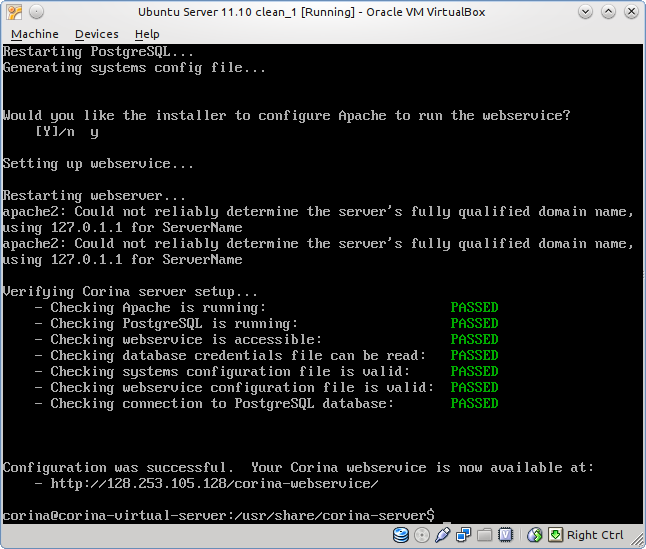
\includegraphics[width=0.48\textwidth]{Images/serverconfig.png}
  \end{center}
  \caption{Screenshot of VirtualBox running the Tellervo server.  The console contains the results of the tests run at the end of the configuration routine.}
  \label{fig:serverconfig}
\end{wrapfigure}

\begin{enumerate}
 \item Open VirtualBox and go to \menutwo{File}{Import Appliance}
 \item Press the choose button and locate the virtual appliance file that you downloaded from the website\footnote{If you are using an older version of VirtualBox it may expect an OVF rather than the OVA file provided.  The OVA file is a tar file containing several files required by VirtualBox including an OVF file.  If you rename the extension of the OVA file to tar then extract the contents to a folder using a tools like WinRAR you should then be able to continue.}
 \item Rename the server if you choose, then press the finish/import button
 \item Once the server is installed, highlight it in the virtual machine list and press the `settings' button
 \item Go to `Network' and choose `Attached to Bridged Adapter'.  You may also like to give the system more RAM if you have powerful machine
 \item Click ok, then back on the main page, press the `run' button
 \item Read and accept the information about how to gain and release control of the keyboard in VirtualBox
 \item The server will boot and eventually present you with a command line login screen.  Log in with the following temporary details:
    \begin{description}
      \item[Username] : tellervo
      \item[Password] : dendrochronology
    \end{description}
 \item Once you are logged in the server will automatically ask you a series of questions 
 \item Answer the questions and the configuration will finish by testing your new server (see figure \ref{fig:serverconfig}). 
 \item Note down the URL of your new Tellervo webservice as you will need to enter this when you start your Tellervo desktop client.  If you need to know the URL at a later date you can run the tests again by typing: \code{tellervo-server --test}
 \item You can now install and run the Tellervo Desktop application (see section \ref{txt:desktopinstall})
\end{enumerate}

To save on download size and disk space only the essential packages to make the server run have been installed.  This means there is no graphical interface just a command line.  Hopefully this should not be a problem as once set up, the only interaction needed with the Virtual Appliance will be through the normal Tellervo desktop application.  If you would prefer to use a graphical interface to the server this can be easily installed.  See chapter \ref{txt:servermaintenance} for further details.

There are a number of limitations caused by distributing the server software in this way. The operating system has already been configured to use networking without a proxy server, so if your computer requires a proxy then you won't be able to connect to the Internet.  Please contact the developers for more details.

VirtualBox has a number of methods for providing network connectivity to the Tellervo virtual appliance.  The default setup described above is to use \textbf{bridged networking}.  This makes the virtual server appear as if it was another physical computer on your network with its own IP address.  This works best in most situations, but can cause problems if your network administration is particularly strict.  It is also not suited to those installing Tellervo Server on a laptop which is used on different networks, especially via wifi.  If you have problems with bridged networking, then it may be better to use one of the alternatives listed below.

The first network alternative is to use \textbf{host-only networking}.  To use this you simple select your server in VirtualBox, click settings then on the network tab choose host-only adapter.  This setting means that your server will only be visible to the physical computer you are running Tellervo server on.  This may not be a problem (it may even be desirable) if you are installing for your personal use but of course it is not suitable if you are intending to share the server with colleagues.

The second network alternative is to use \textbf{NAT networking}.  NAT stands for Network Address Translation and means that requests and responses sent to/from your physical computer are intercepted and forwarded on to the virtual Tellervo server.  Instead of Tellervo server having its own IP address, Tellervo clients wanting to talk to the server send requests to your physical computer.  This has the benefit of being more likely to work if your institution has strict network policies.  The main drawback is that it takes a little more effort, and perhaps requires a better understanding of systems administration to set up.  

With your virtual machine powered off, select it in VirtualBox, click settings and go to the network tab.  Change the network type to NAT and then click the port forwarding button.  Add an entry to the list:
\begin{description}
 \item[Name] - TellervoHTTP
 \item[Protocol] - TCP
 \item[Host Port] - 8080
 \item[Guest Port] - 80 
\end{description}
You can leave the other fields blank.  The host port is the port that your Tellervo users connect to.  The normal port that users connect to for web services is port 80, however, on most secure operating systems (e.g. Linux and OSX) you cannot port forward to ports below 1024, although it should be possible in Windows.  If you are running Windows you may therefore be able to use a host port of 80.  If you use 8080 (or any other port other than 80) you will need to include this in the URL of your webservice when you try to connect.  The other complication of using NAT networking is that the URL provided by the Tellervo server configuration utility is incorrect as the server has no way of knowing that NAT is being used.  The URL that you need to use to connect to is: \url{http://ip.of.your.physical.machine:8080/tellervo/}  


\subsection{Ubuntu native installation}
\label{txt:installnativeserver}
If you are fortunate enough to be running Ubuntu then the native Ubuntu deb package is the best and easiest method for installing the Tellervo server, otherwise see section \ref{txt:virtualAppliance} to install the server as a Virtual Appliance.  

To install the Tellervo server in Ubuntu simply download the deb package from the Tellervo server \url{http://www.tellervo.org/download} and install with your favourite package manager.  For instance, to install from the command line simply type: \code{sudo dpkg --install tellervo-server.deb}.  If you haven't got all the required dependencies already installed dpkg will return an error.  This can be fixed by running \code{sudo apt-get install -f} which will install all the missing packages, and will automatically allow dpkg to run to completion.  

The package will automatically run a configuration script to assist with creating a database user, building the Tellervo PostgreSQL database, setting database permissions and setting up the Apache webservice.  The configuration ends with a test routine to check all services are set up correctly and if so, will provide you with the URL of the newly configured Tellervo webservice.

\subsection{Advanced install on other operating systems}
\label{txt:installadvancedserver}
As mentioned previously, the limited resources available for Tellervo development means that we have been unable to produce native installers for platforms other that Ubuntu.  The VirtualBox method can be used on all modern operating systems so we strongly suggest you stick with this method.  However, if you are an experience systems administrator and are feeling brave, it is possible to set up the Tellervo server manually.  

\index{Dependencies!Server}
The Tellervo server is essentially a PostgreSQL database accessed via a PHP webservice running on Apache 2.  The following dependencies are therefore required: postgresql-9.1; postgis; postgresql-contrib-9.1; postgresql-9.1-pljava; sun-java6-jre; apache2; php5; php5-pgsql; php5-curl; php5-mhash.

The basic procedure for installation is as follows:

\begin{itemize*}
 \item Install all dependencies
 \item Create PostgreSQL database from Tellervo template SQL file
 \item Set up a database user and provide access to the server in the pg\_hba.conf file
 \item Give this user read and write permissions to the database
 \item Copy the webservice code into a web accessible folder
 \item Set up Apache to see this folder by creating an entry in the sites-enabled folder
 \item Restart PostgreSQL and Apache and check you can access the webservice from a web browser
\end{itemize*}




\section{Installing the desktop application}
\label{txt:desktopinstall}
\index{Installation!Desktop application}
Installation packages for the Tellervo desktop application are available for Windows, MacOSX and Ubuntu Linux.  Tellervo can also be run on other operating systems as long as they support Java 6 or later\footnote{Tellervo was initially developed against Sun Java 6 JRE, however, now OpenJDK6 is routinely used.  See section \ref{txt:java}, page \pageref{txt:java} for more information.}.

To install Tellervo, download the installation file for your operating system from \url{http://www.tellervo.org/download}. The website should provide you with a link to the installer for your current operating system:

\begin{description}
\item 
\includegraphics[width=3mm]{Images/windows.png} \textbf{Windows} -- Run the setup.exe and follow the instructions. If you do not have Java installed the installer will direct you to the Java website where you can get the latest version. Once installed, Tellervo can be launched via the Start menu.  Please note that Windows (and possibly also your anti-virus software) may warn you that the installation program is not commonly downloaded and may be dangerous.  You will see that the installation package is digitally signed by the University of Arizona indicating that the file has not been tampered with.  As long as you trust the Tellervo developers you can safely install the program.

\item 
\includegraphics[width=3mm]{Images/mac.png} \textbf{Mac OS X} -- As mentioned above, Tellervo requires Java 6. Although MacOSX ships with Java installed, unfortunately Apple have been very slow to provide Java 6. Although it was released in 2006, it was not until August 2009 that Apple made Java 6 available as part of v10.6 (Snow Leopard). Tellervo can therefore only be run on Snow Leopard or later\footnote{The Snow Leopard requirement for Mac computers means that Tellervo cannot be run on older PowerPC-based MacOSX computers.  However, if you have old PowerPC iMacs you could consider replacing the operating system with a modern Linux distribution like Ubuntu.  Linux continues to support PowerPC architecture even in the most recent releases.  You will of course not be able to run any of your other exisiting MacOSX software.}. To install Tellervo, download then open the zip file and drag the Tellervo.app into your applications folder.  To use the 3D mapping or measuring platform hardware in Tellervo you will also need to install the `Tellervo Drivers' package.  Note that users of OSX 10.8 (Mountain Lion) and later may be told that the package is broken.  This is due to Apple's new GateKeeper tool which by default won't allow non-Apple unsigned applications to run.  See section \ref{txt:malware} for more information.   

\item 
\includegraphics[width=3mm]{Images/ubuntu.png} \textbf{Ubuntu Linux} --  A deb file is available which was designed for use on Ubuntu distributions but should work on any Debian based system. Install using your favorite package management system or from the command line like this: e.g. \code{sudo dpkg --install tellervo.xx.xx\_all.deb} On Ubuntu and similar distributions, the package should add a Tellervo shortcut to your applications menu. Alternatively you can start Tellervo from the command line by typing tellervo.  For other Linux distributions you are probably better off using the standard Java executable described below.  Note though that you will need to manually install serial port and 3D graphics libraries to use these features in Tellervo.  If there is demand for a package for other Linux distributions we may make these available in the future.  For instance, basic RPMs have been produced but we do not have the time or resources to test these at the moment.

\item 
\includegraphics[width=3mm]{Images/java.png} \textbf{Other operating systems} -- Make sure you have Java 6 installed, then download the Tellervo jar file to your hard disk. You can run Tellervo from the command line by typing: \code{java -jar tellervo.jar}  Note that several native libraries are required to enable Java to interface with your serial port and 3D graphics hardware.  If you want to take advantage of these features in Tellervo you will need to manually install these libraries.  Please contact the Tellervo developers for more information.
\end{description}

Once you have installed your Tellervo Desktop application and you have access to a Tellervo server you are now ready to launch Tellervo for the first time.


\subsection{Malware and broken package warnings}
\label{txt:malware}

The MacOSX package for Tellervo is currently `unsigned'.  By default any application run on MacOSX Mountain Lion (10.8) and later must be signed with an Apple certificate to run.  Rather frustratingly rather than explain this OSX simply reports that the package is `damaged'.

The cleanest method for fixing this is for us (the developers) to pay a certificate from Apple.  However, with tight budgets all around, justifying spending hundreds of dollars each year just to digitally sign the installation packages is very difficult.  Until we find the funds to do this sustainably, you will need to change some security settings.  First, go to \menutwo{System Properties}{Security and Privacy}.  By default it is set to allow applications from `Apple and known developers'.  You will need to change this to `any developer' to be able to run Tellervo. With this set, when you run Tellervo you will be warned that the package is untrusted but it will then allow you to proceed.


\subsection{First time launch}
\index{Wizard, Setup}
When you launch Tellervo for the first time you will be presented with a setup wizard (figure \ref{fig:setupwizard}).  Following the wizard to configure the main settings required before you can begin to use Tellervo.  If you want to re-run this wizard at any time you can do so from the entry in the Help menu. You can also manually edit all these settings from the Tellervo preferences dialog which can be found in \menutwo{Edit}{Preferences}.

\begin{figure}[hbtp]
  \centering
    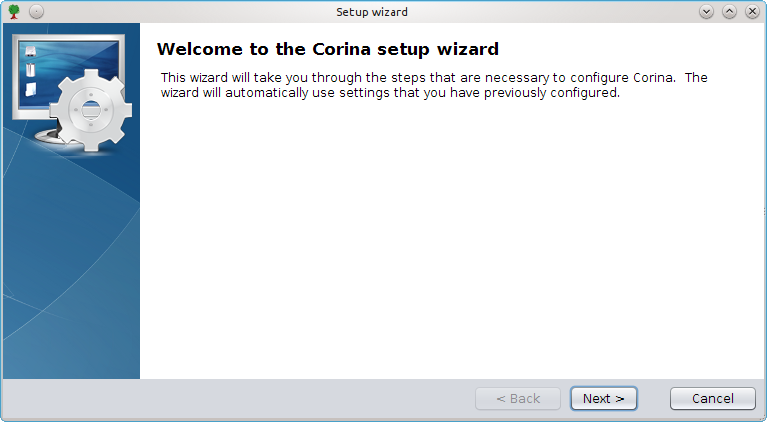
\includegraphics[width=0.6\textwidth]{Images/setupwizard.png}
  \caption{The Tellervo setup wizard will launch the first time you start Tellervo.}
  \label{fig:setupwizard}
\end{figure}

The pages of the wizard include:

\begin{description}
 \item[Network connection] -- this configures how your computer accesses the internet.  Most users will be able to use the default `Use system default proxy settings' option here, but if you know that your computer is behind a corporate proxy server you may choose to manually provide the settings.
 \item[Configuring the Tellervo server] -- Tellervo comes in two parts: the Tellervo desktop client that you are using; and the Tellervo server which runs the database that stores your data.  If you are working in a lab your systems administrator may have already set up the Tellervo server and given you the URL to connect to.  Alternatively, you may have already installed the Tellervo server yourself.  If so the installation program should have given you the URL. If you don't want to take advantage of the full capabilities of Tellervo you can opt to disable database integration.  If you do not configure a Tellervo server you will be left with a basic file-based dendro data collection tool.
 \item[Measuring platform configuration] -- the next page enables you to configure measuring platform hardware attached to your computer.  Some measuring platforms have fixed settings in which case the port settings will be set automatically, but others can be changed in the hardware and must be set explicitly here. Use the `Test Connection' button to make sure that Tellervo can successfully communicate with your platform.
 \item[Tutorial videos] -- Once you've completed the wizard you will be given the option of viewing tutorial videos explaining how to use Tellervo.  You can access these at any time via the Help menu or through the Tellervo website.
\end{description}


Assuming that you have configured a Tellervo server, once you have finished the wizard you will be presented with a login dialog (figure \ref{fig:login}).

The username and password details requested are your Tellervo login credentials (not your system or network credentials) provided to you by your systems administrator.  If you are using your own Virtual Appliance server, the default admin user details are provided in section \ref{txt:passwords}, page \pageref{txt:passwords}.  The dialog gives you the option for saving your username and/or password if you prefer.  We recommend using this feature only on personal machines.  You may choose to cancel the login if you like and Tellervo will continue to load, however, you will not have access to the Tellervo database therefore very few functions will be available to you.

\begin{wrapfigure}{r}{0.5\textwidth}
  \begin{center}
    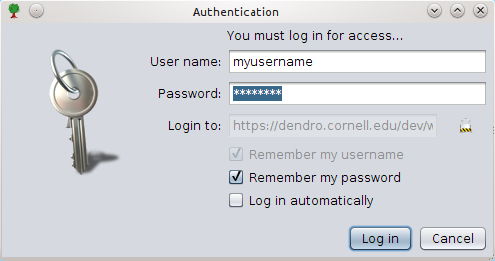
\includegraphics[width=0.48\textwidth]{Images/login.png}
  \end{center}
  \caption{Tellervo server login dialog.}
  \label{fig:login}
\end{wrapfigure}

Once you have logged in you will be presented with the Tellervo home screen.  This contains the main menus for the program as well as quick-link icons for creating new records, opening existing records and importing existing data files to the database.


\subsection{Mapping support}
\index{Mapping}
Tellervo includes 3D mapping for visualization of sampling locations. Although this is not necessary for most tasks, to make use of the mapping functions you will require a OpenGL 3D capable graphics card. To check whether your computer already supports 3D mapping, open Tellervo, go to Admin, then Site map.  Tellervo will warn you if your graphics card is not supported.

All MacOSX computers should automatically support OpenGL.  Most Windows and Linux computers made since 2006 should also support OpenGL, however, this does require proper drivers to be installed. In some cases Windows computers may include a compatible graphics card, but may only have the default Windows video drivers installed.  If you are having trouble with the mapping in Tellervo make sure you have installed the most recent drivers for your graphics card.  Linux users may be required to install proprietary graphics drivers.  

The mapping component of Tellervo makes use of NASA's open source World Wind Java.  NASA's website \url{http://worldwind.arc.nasa.gov/} contains further information and instructions that you may find helpful if you are having problems getting the mapping to work.  


\section{Upgrading Tellervo desktop}

There are no special requirements for upgrading the Tellervo desktop client.  You need simply install the new version over the top of your previous version.  Any personal settings will be maintained after the upgrade.


\section{Upgrading Tellervo Server}

The process for upgrading your server is the same regardless of whether it is running in a VirtualBox virtual machine or on a native Linux server.  As with any upgrade, the first thing you need to do is backup your data (see section \ref{txt:BackupVA}, page \pageref{txt:BackupVA}).  We cannot be held responsible for loss of data in the event something goes wrong during the upgrade process.  

Open your Tellervo server and log in to the command line.  Then type the following commands:

\code{cd /tmp}
\code{wget http://www.tellervo.org/url-of-the-updated-package.deb}
\code{sudo dpkg --install tellervo.x.x.x.deb}

The first line changes your current directory to the temporary folder.  The second command downloads the new package from the Tellervo server.  Make sure you enter the correct URL to the package you are upgrading to.  The final command installs the new package.  Again make sure you have the correct file name specified here. If all goes well, your webservice and database will be upgraded to the latest version and the server test routine will run to confirm all is correct.  If the server gives you any errors or warnings, please contact the developers for further assistance.

\section{Uninstalling}

We understand that Tellervo will never suit the requirements of all users, but as an open source product, we would really appreciate feedback as to why it didn't work for you.  Without this feedback it is difficult to prioritize future development.

\subsection{Tellervo desktop application}
For Windows users, Tellervo desktop can be uninstalled using the standard add/remove programs feature in control panel, or via the item in the Tellervo start menu.  Mac users should simply delete the application from their applications folder.  Linux users should use their prefered package management tool e.g.\ from the command line:
\code{sudo dpkg --remove tellervo}

\subsection{Tellervo server}

\warn{Please note that uninstalling the Tellervo server will delete your Tellervo database and all the data it contains.  Make sure that you export any data you need before doing uninstalling.}

If you are running the Tellervo server as a virtual appliance simply follow the uninstall instructions for VirtualBox.  If you are running Tellervo server as a native Linux server, you should use your preferred package mangement tool e.g.\ from the command line:
\code{sudo dpkg --remove tellervo-server}








    
\chapter{Getting started}
\label{txt:gettingstarted}

Once you have your Tellervo desktop application installed (see chapter \ref{txt:installation}) and you also have access to a Tellervo server (either via your lab network administrator or your own on as a Virtual Appliance) you are ready to start using Tellervo.  Below are some basic instructions for performing common tasks in Tellervo followed by a number of more in-depth chapters.  If you are running Tellervo with database integration disabled (Tellervo-lite mode) then see section \ref{txt:tellervolite} for further details.

\section{Measuring a new sample}
\index{Sample!Measuring|(}
\label{txt:new}
Once your measuring platform has been configured, measuring your first sample is simple.  To start a new measurement go to \menutwo{File}{New} or click the `new' icon on the home screen. A dialog will appear where you can scan your sample's barcode, or press the button to enter metadata for your sample later. Barcodes minimize data entry errors and also speed up the process of measuring your samples. See section \ref{txt:barcodes} for more information. Once you have scanned your barcode or pressed the button, you will then be presented with an empty Tellervo metadata screen.

The next step is to fill out the metadata information. If you have used a barcode, nearly all of this metadata will be filled in for you, otherwise you will need to fill this out yourself. Details about metadata can be found in chapter \ref{txt:metadata}, page \pageref{txt:metadata}.  Once you have populated the metadata tab, you can then switch to the data tab (figure \ref{fig:datascreen}).  

\begin{figure}[hbtp]
  \centering
    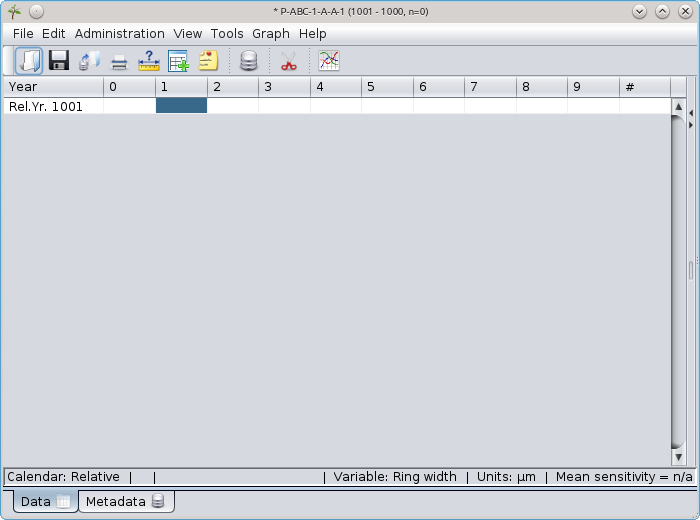
\includegraphics[width=0.6\textwidth]{Images/datascreen.png}
    \caption{An empty data window ready to receive measurements.  Note the status bar at the bottom includes buttons for changing the measurement variable, display units and cumulative statistics.  The data table stores ring width values in decadal rows following the standard convention which derives from data entry via punch-cards.  Undated sequences begin in the relative year 1001 for the same reason.}
    \label{fig:datascreen}
\end{figure}

Before you begin measuring you need to tell Tellervo what sort of measurements you are making: whole ring widths; or early/latewood widths (the default is whole ring widths).  To specify early/latewood widths you need to go to \menuthree{Edit}{Measuring mode\ldots}{Early and latewood widths}.  If you use this menu after you have already measured some rings you will be warned that Tellervo will delete the data you have already collected.  Once in `early and latewood widths' measuring mode you will be able to choose which data is displayed in the table by clicking the variable box on the status line and choose between: Ring width; Earlywood width; Latewood width; Early/Latewood width.

To begin measuring your sample you can now go to \menutwo{Edit}{Start measuring}, press the start measuring button on the toolbar, or you can press F5. While measuring you should be provided with audible feedback for each ring measured with a more pronounced sound made every 10th ring. If there is a problem communicating with your measuring hardware, check your settings in the preferences dialog. If you still have problems contact the Tellervo developers by going to \menutwo{Help}{Report bug on last transaction}, making sure you include your email address and any further information.

If your sample is already dated and/or you already know how many rings your sample has, then you can initialise your data matrix using the button on the toolbar.  This gives you a dialog requesting date and ring number information which can be useful for those of you that use the skeleton plotting method prior to measuring.  

Note by default Tellervo labels rings as relative years beginning in 1001.  If your sample is dated, you should explicity tell Tellervo either using the initialise grid function prior to measuring, or by going to \menutwo{Tools}{Redate} once you've finished.

Depending on the measuring platform hardware you have, you will see some variation of the measuring panel in figure \ref{fig:measurepanel}. The left display holds the absolute position of the last ring boundary (for device that measure cumulatively), the middle display holds the last recorded measurement width and the right display holds the current position of the measuring plaform (for devices that report live measurements).  The right-hand display is useful for devices that don't have a physical display such as the Lintab. 

\begin{wrapfigure}{r}{0.5\textwidth}
  \begin{center}
    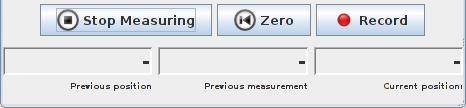
\includegraphics[width=70mm]{Images/measurepanel.png}
  \end{center}
  \caption{Measuring control panel.}
  \label{fig:measurepanel}
\end{wrapfigure}


Tellervo supports the measuring of rings both individually and cumulatively.  We feel that it is easier and more accurate to measure rings individually, that is to say the device is reset to zero after each measurement.  If a device accepts requests to reset measurements (e.g.\ Quadra Chek boxes) or if it automatically resets itself to zero after recording a measurement (e.g.\ EVE IO) then this procedure is used by Tellervo.  In this case the user begins measuring by setting the display to zero, then turns the platform to the end of the ring, then either presses the `measure' button on the hardware device or the `record' button on the screen.

\tip{If your device does not have a physical `measure' button you don't need to click on the `record' button each time.  Instead click on the `turn on mouse trigger' button and then you can use your mouse's left button as a measure button regardless of where the mouse is on the screen. This means you don't need to lift your eyes from your microscope to ensure you are clicking the button correctly.  When you're finished measuring press escape to exit this mode.}

Certain devices (e.g. Boekler Microcode boxes) do not listen for requests to reset to zero.  In this case to measure each ring individually, you would need to manually reset the reading to zero following each measurement.  This would of course be extremely tedious.  In this situation Tellervo measures cumulatively from the beginning of the first ring and calculates the ring width based on the previous ring boundary position.  With this method you must be careful not to knock your sample, and you must also take special care when altering radii to navigate around problem structures.  If you do knock your sample, the best way to recover is to reset your platform to zero and press the measure button.  Next, press the `stop measuring button', manually fix the values in the data table, then begin measuring again from where you left off.

If you are in `Early and latewood widths' measuring mode the measurements are made and sent to the data table in pairs.  The first measurement should be of the earlywood of the ring, and the next value the latewood measurement.  Whether you are currently measuring early or latewood is indicated as a message at the bottom of the measuring panel.

\index{Ring remarks}
While you measure your sample you can flag features in a ring by right clicking on any cell in the table and selecting one or more of the standard notes (see figure \ref{fig:ringremarks}).

Tellervo supports all standard TRiDaS remarks including: fire damage; frost damage; crack; false ring(s); compression wood; tension wood; traumatic ducts; single pinned; double pinned; triple pinned and many others.  Rings that include remarks are indicated by the relevant icon in the data screen.  Depending on your method of work, this can be useful for keeping track of sample pin holes.  For instance, if a missing or false ring is discovered after a sample has been pinholed, the offset in pinholes can be easily seen without resurfacing the sample.  

\begin{wrapfigure}{r}{0.5\textwidth}
  \begin{center}
    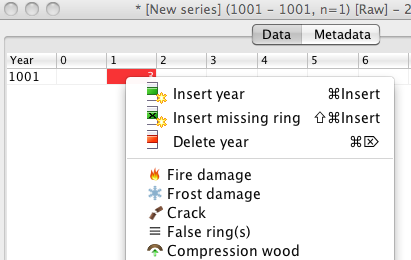
\includegraphics[width=0.42\textwidth]{Images/ringremarks.png}
  \end{center}
  \caption{Right click context menu showing some of the options for adding remarks to rings.}
  \label{fig:ringremarks}
\end{wrapfigure}

In addition to the right click menu, you can also access ring remarks by opening the remarks panel using the button on the toolbar.  This panel gives the the ability to add free text remarks to individual rings.  One final method for adding remarks is specific to fire history researchers.  Standard FHX-style remarks can be added to rings by pressing the equivalent FHX character code key in the relevant ring cells.  For instance pressing a lower-case `a' in a cell will add the `fire injury in latewood' remark.   

The data screen also contains a status bar at the bottom. By clicking on the units section, you can switch between micron and 1/100th mm units. Tellervo understands the units being supplied by the measuring platform, therefore changes here are purely for display purposes only. If you have a platform that measures in microns, but prefer to see the values in 1/100th mm then you can use this feature.  There are also options on the status bar that enable you to choose one of a variety of summary statistics about your series.

Once you have finished measuring your sample, you should then go to \menutwo{File}{Save} to save your series to the database. 
\index{Sample!Measuring|)}


\section{Opening existing data}
\index{Sample!Opening}
\label{txt:open}
If you have used traditional dendrochronology software, you are probably used to opening existing dendro data files from your computer.  Tellervo works in a different way.  All data accessed by Tellervo is stored within the central Tellervo database rather than in files.  The database provides many benefits over file based storage, most importantly it means there is a high degree of security and integrity in your data.\footnote{This doesn't mean you don't have to backup your data though!  Whoever is in charge of maintaining your Tellervo database should make sure regular backups are made--preferably offsite.}

To use data that you have stored in existing data files you must first \emph{import} your data into the Tellervo database.  This gives you the opportunity to clean-up your data!  For details of how to import your data see chapter \ref{txt:importExport}, page \pageref{txt:importExport}.

Once you have data in your database, either by importing existing data files or measuring new samples, you can access your data through the database browser.  This is accessed through the \menutwo{File}{Open} or \menutwo{File}{Open multiple} menus and an example of the dialog is shown in figure \ref{fig:dbbrowser}. The same database browser dialog is used in multiple places throughout Tellervo, e.g.\ when adding addition series to graphs and when choosing chronologies to crossdate against. 

\begin{figure}[hbtp]
  \centering
    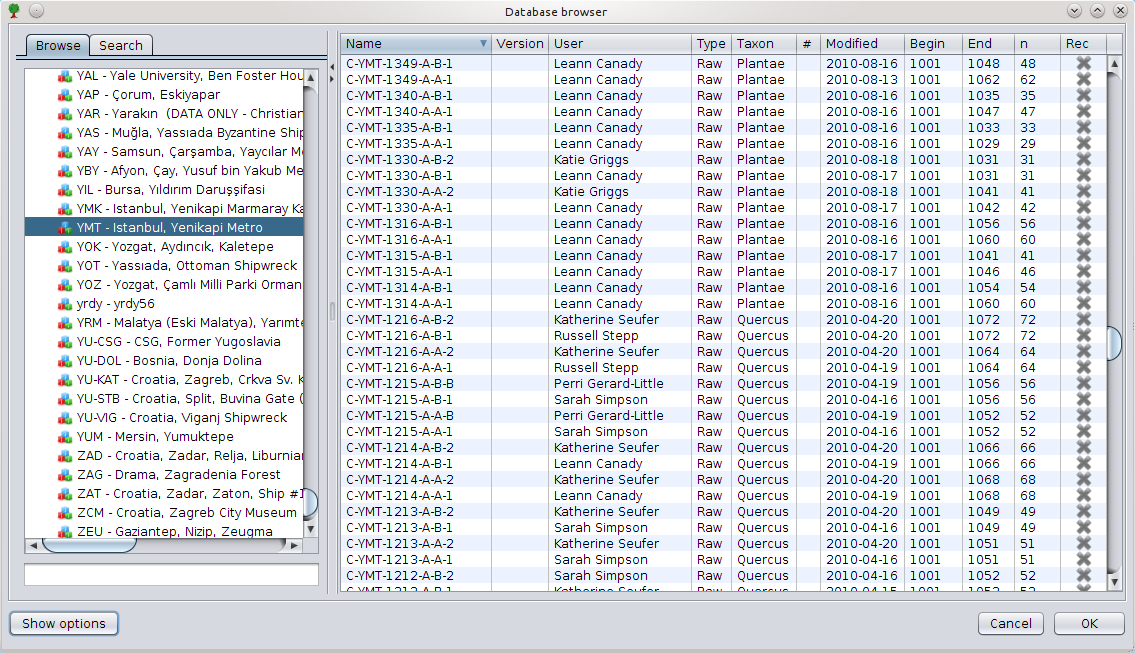
\includegraphics[width=0.9\textwidth]{Images/dbbrowser.png}
    \caption{Screenshot of the database browser dialog.}
    \label{fig:dbbrowser}
\end{figure}

The database browser is divided into two main parts.  On the left is the browse and search tabs, and on the right is the series table.  Selecting options in the browse or search tab populates the series table on the right with all the series that match the specified criteria.  

\warn{The search tab is currently a `work-in-progress' so we recommend you use the browse tab until further notice.}

The browse tab shows a heirarchical tree view of the contents of your Tellervo database based upon the TRiDaS data model.  The panel will be pre-populated with all the objects in your database but it is possible to `drill-down' by right clicking on an object and choosing `Expand branch'.  Expanding an object for instance, will show all the elements associated with that object, and expanding an element will show all the samples associated with the specified element.  To better understand the TRiDaS terminology please read chapter \ref{txt:metadata}, page \pageref{txt:metadata}.

By double clicking (or right clicking and choosing `Search for associated series') on an item in the browse panel Tellervo will search the database for all series that are associated with the specified entity.  The results of the search will be shown in the series table on the right of the screen.  This table shows basic metadata about each search and is sortable by click on any of the column headers.  To open a series, simply select one of these series and click `OK'.  If the database browser is open in 'multiple series' mode, then you can use the arrow buttons to select multiple series to open in one go.

There is also a `Show options' button on the database browser dialog.  This adds additional advanced methods for filtering the series table to help you find the data you are interested in.

\section{Reconciling data}
\index{Sample!Reconciling}
Tellervo has been developed not only for experience dendrochronologists, but as a tool for teaching students.  It therefore includes a comprehensive `reconciling' tool for supervisors to check the quality of measurements made by students.  The reconcile dialog does a comparison of a measurement series made by a student with a references series of the same radius measured by the supervisor.  The same dialog can also prove useful for comparing measurements from two experienced dendrochronologists when handling particularly difficult samples.


\section[Tellervo-lite]{Tellervo-lite: running without database server integration}
\label{txt:tellervolite}
\index{Tellervo-lite}
\index{Offline mode}
When you run Tellervo with database integration disabled (referred to as Tellervo-lite), you are presented with a simplified interface without database functionality. Tellervo-lite has basic measuring functionality only and does not take advantage of many of the advanced features introduced by the full Tellervo application.  We strongly recommend installing Tellervo server to take advantage of all that Tellervo has to offer.

When reading this manual please keep in mind that for the most part it is assuming that you are using the full Tellervo application.  Although in some cases the information is useful regardless of whether you're using Tellervo or Tellervo-lite, there will be differences, and of course features that require the database (such as mapping, user permissions and analysis tools) that will be disabled or missing entirely.  

Instead of opening and saving data to the Tellervo database, in Tellervo-lite data is accessed via traditional data file formats such as Tucson, Heidelberg and Sheffield etc.  In Tellervo-lite, \menutwo{File}{Open} presents the user with a standard file dialog box rather than the Tellervo database browser.  Similarly when the user clicks \menutwo{File}{New}, instead of being presented by the barcode dialog, they are taken directly to the data editor (with a limited metadata tab).   

Tellervo-lite is a departure from the primary mission of Tellervo (i.e.\ to provide a user-friendly application that supports standardised dendro data and metadata). The support for metadata in legacy dendro file formats ranges from non-existent to minimal with little standardisation.  Given the wide variation in metadata that can potentially be provided by these formats, it is not practical to support reading and editing in Tellervo-lite, instead it provides a very minimal interface for recording non-standardised metadata.  This basic metadata screen replaces the TRiDaS-based metadata interface normally seen in the standard version of Tellervo.  How this basic metadata is used (or indeed whether it is used at all) depends on the file format you choose to save to.  

When opening legacy dendro files in Tellervo-lite, it is possible that metadata will be discarded.  So if you open and edit an existing file in Tellervo, then overwrite the orignal you may well loose information.  We highly recommend saving changes to a different file.  It is also important for users to understand the limitations of the file formats you're reading from and writing to.  For instance the Tucson format has no mechanism for indicating whether years are absolute or relative so data loaded from Tucson files will be marked as relative years in Tellervo.  Some formats also store ring-width measurements in 1/100th mm integers, so if you measure in microns then the values will be rounded. A full description of each format along with their limitations is given in appendix \ref{txt:fileFormatsStart}.







    %\chapter{Measuring samples}
\index{Sample!Measuring|(}
Although it is possible to manually enter the ring widths of your samples into Corina, it is normal to automate this process using a measuring platform. Corina supports the most common measuring platforms including Velmex and Lintab.  For details on how to configure your measuring platform see section \ref{txt:MeasuringPlatformConfig}.

Once your measuring platform has been configured, measuring your first sample is simple.  To start a new measurement go to \menutwo{File}{New} or click the `new' icon on the home screen. A dialog will appear where you can scan your sample's barcode, or press the button to enter metadata for your sample later. Barcodes minimize data entry errors and also speed up the process of measuring your samples. See section \ref{txt:barcode} for more information. Once you have scanned your barcode or pressed the button, you will then be presented with an empty Corina data screen (figure \ref{fig:datascreen}).

\begin{figure}[hbtp]
  \centering
    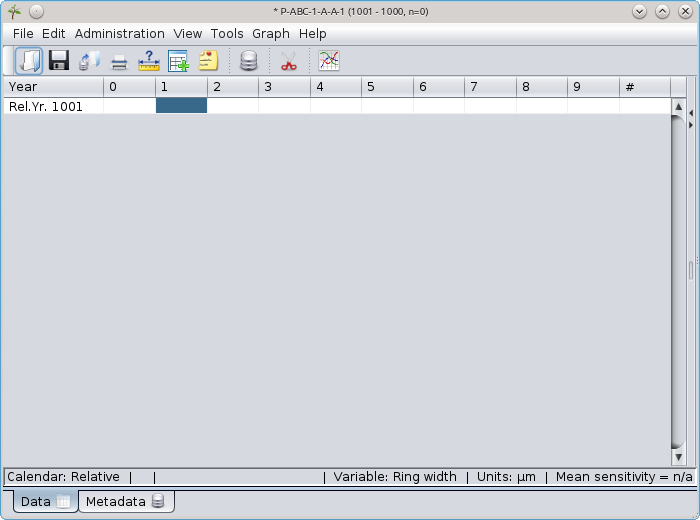
\includegraphics[width=0.6\textwidth]{Images/datascreen.png}
    \caption{An empty data window ready to receive measurements.  Note the status bar at the bottom includes buttons for changing the display units and cumulative statistics.}
    \label{fig:datascreen}
\end{figure}

The next step is to fill out the metadata tab. If you have used a barcode, nearly all of this metadata will be filled in for you, otherwise you will need to fill this out yourself. Details about metadata can be found in chapter \ref{txt:metadata}, page \pageref{txt:metadata}.

To begin measuring your sample you can now go to \menutwo{Edit}{Start measuring} or you can press F5. Depending on the type of platform you have you will have different buttons available at the bottom of the screen.  If you platform accepts requests for measurement data, or accepts requests to zero the measurement then you will have buttons available to do so.  Otherwise you will need to use the hardware buttons on your device to send measurements to Corina.

While measuring you should be provided with audible feedback for each ring measured with a more pronounced sound made every 10th ring. If there is a problem communicating with your measuring hardware, check your settings in the preferences dialog. If you still have problems contact the Corina developers by going to \menutwo{Help}{Report bug on last transaction}, making sure you include your email address and any further relevant information.


\index{Ring remarks}
While you measure your sample you can flag features in a ring by right clicking on any cell in the table and selecting one or more of the standard notes (see figure \ref{fig:ringremarks}).

\begin{wrapfigure}{r}{0.5\textwidth}
  \begin{center}
    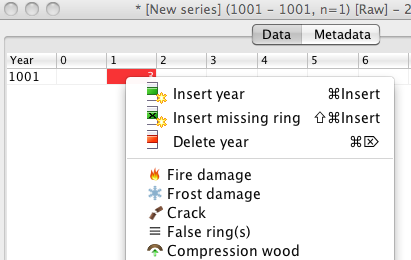
\includegraphics[width=0.48\textwidth]{Images/ringremarks.png}
  \end{center}
  \caption{Right click context menu showing some of the options for adding remarks to rings.}
  \label{fig:ringremarks}
\end{wrapfigure}

Corina supports all standard TRiDaS remarks including: fire damage; frost damage; crack; false ring(s); compression wood; tension wood; traumatic ducts; single pinned; double pinned; triple pinned and many others.  Rings that include remarks are indicated by the relevant icon in the data screen.  Depending on your method of work, this can be useful for keeping track of sample pin holes.  For instance, if a missing or false ring is discovered after a sample has been pinholed, the offset in pinholes can be easily seen without resurfacing the sample.  In the future Corina will also include support for user defined ring remarks.  

The data screen also contains a status bar at the bottom. By click on the units section, you can switch between micron and 1/100th mm units. Corina understands the units being supplied by the measuring platform, therefore changes here are purely for display purposes only. If you have a platform that measures in microns, but prefer to see the values in 1/100th mm then you can use this feature. At the bottom ring of the status bar you can choose one of a variety of summary information about your series.

Once you have finished measuring your sample, you should then go to \menutwo{File}{Save} to save your series to the database. 

\section{Reconciling data}
\index{Sample!Reconciling}
Corina has been developed not only for experience dendrochronologists, but as a tool for teaching students.  It therefore includes a comprehensive `reconciling' tool for supervisors to check the quality of measurements made by students.  The reconcile dialog does a comparison of a measurement series made by a student with a references series of the same radius measured by the supervisor.  The same dialog can also prove useful for comparing measurements from two experienced dendrochronologists when handling particularly difficult samples.

 

\index{Sample!Measuring|)}

    \chapter{Measuring platforms}
\label{txt:MeasuringPlatformConfig}
\index{Measuring platforms}
\index{Hardware|see{Measuring platforms}}

Although it is possible to manually enter the ring widths of your samples into Tellervo, it is normal to automate this process using a measuring platform. Tellervo supports the most common measuring platforms including Velmex and Lintab.  However, please note that standard Lintab platforms use a proprietary communications protocol. Rinntech--the manufacturers of Lintab platforms--claim intellectual property rights over this protocol. During discussions between the Tellervo development team and Rinntech an agreement was reached whereby the Tellervo developers agreed not to release details of the protocol. In turn Rinntech has agreed to produce an adapter that can be attached to Lintab platforms so that they communicate with an open ASCII protocol. Users wishing to use Lintab platforms with Tellervo (or any software not developed by Rinntech) must therefore contact Rinntech and purchase an adapter.

Measuring platforms typically use serial ports to communicate to computers. In recent years computer manufacturers have been phasing out serial ports so you may need to purchase a serial-USB converter. Modern MacOSX, Linux as well as Windows 7 should support most serial-USB adapters out of the box, otherwise you must install the relevant drivers before continuing.  Recent Lintab USB platforms use internal serial-USB converters so are treated in exactly the same way by Tellervo.

To begin, shut down your computer, attach your platform, then reboot and launch Tellervo. Next, go to the preferences window and open the hardware tab and you should see an interface that looks like figure \ref{fig:hardwareprefs}.

\begin{figure}[hbtp]
  \centering
    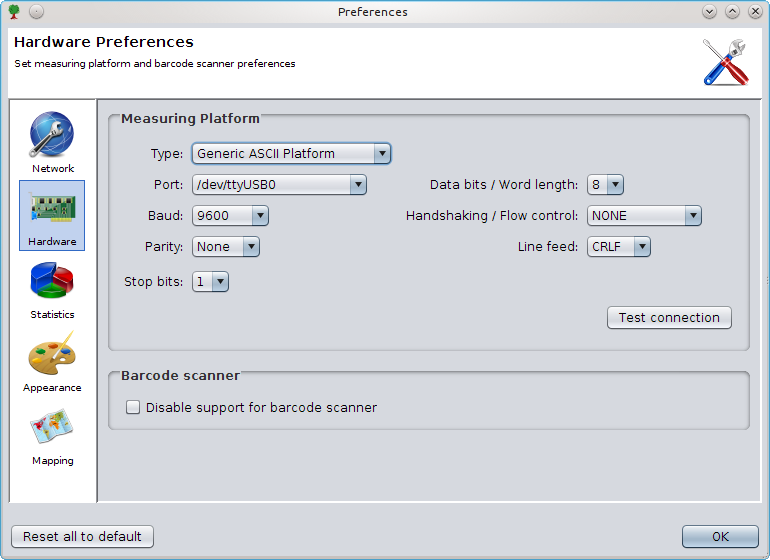
\includegraphics[width=0.6\textwidth]{Images/hardwareprefs.png}
    \caption{The hardware preferences dialog.}
    \label{fig:hardwareprefs}
\end{figure}

In the type pull down menu, select the type of measuring equipment you are using. Note that this refers to the equipment that the computer is attached to, and not necessarily the measuring platform itself. For instance, Velmex platforms are typically connected through a Metronics digital readout device. Included in this list is the EveIO device which is an open-source device designed for the Cornell Tree-Ring Laboratory. Circuit drawings for this device can be obtained from the Cornell lab to enable Hensen measuring platforms to be used with Tellervo (and other software).  If you measuring platform is not included in the list it should be relatively easy for us to add support so please get in touch and we'll see what we can do.  Alternatively you could implement support yourself (either personally or by employing an independent developer).  Technical details on how to do this are included in section \ref{txtSupportingNewMeasuringPlatforms}, page \pageref{txtSupportingNewMeasuringPlatforms}.  

Next you must choose the port that your platform is connected to from the pull down menu. In Windows this will be a COM port, in Linux and Mac this will be a /dev/xxx port.  Depending on the type of platform you choose, you may also need to set various communication parameters.  If these boxes are enabled, please check the documentation that came with your measuring platform to ensure these values are set correctly.

To check whether your platform is working, click the `Test connection' button (see figure \ref{fig:hardwaretest}) and attempt to measure a few rings.  Different measuring platforms have different capabilities.  For instance, some include a physical switch for firing measurement events, others also include switches for resetting measurements to zero.  Some platforms (e.g. Lintab) also continuously report the measurement values to the computer.  So depending on the hardware you use, Tellervo will present the you with slightly different options.  

\begin{wrapfigure}{r}{0.5\textwidth}
  \begin{center}
    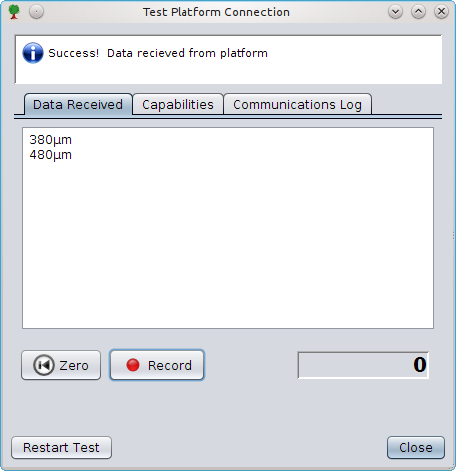
\includegraphics[width=0.48\textwidth]{Images/hardwaretestdialog.png}
  \end{center}
    \caption{Testing the connection to a hardware measuring platform.}
    \label{fig:hardwaretest}
\end{wrapfigure}



The test dialog includes information about the capabilities of your platform as well as a log window to show the raw information being received by Tellervo.  If you are having trouble interfacing with your platform, you should send the communications log to the developers, along with as much information about your hardware as possible.

Once you are satisfied that you are getting the correct results from the measuring platform, click close on the test window and then close the preferences dialog to return to the Tellervo home screen.






    \chapter{Metadata}
\label{txt:metadata}
\index{Metadata|(}
Metadata is `data about data'. In Tellervo this means all the information associated with your physical samples and measurement series e.g. species, location, who measured it, dimensions, slope, soil type etc.

The metadata in Tellervo, and in fact the entire Tellervo data model, is based on the Tree Ring Data Standard (TRiDaS)\footnote{The metadata described in this chapter refers to the full version of Tellervo.  If you are using Tellervo-lite (i.e. Tellervo without database integratiopn) the metadata interface will be replaced with a very basic metadata panel for saving non-standard information to legacy dendro data files.  Please see section \ref{txt:tellervolite} for more information.}. Before you use Tellervo you may find it useful to read \citet{tridas} so that you get a better understanding of the principles of TRiDaS, but a summary is also provided here.

\section{Tree Ring Data Standard - TRiDaS}
\index{TRiDaS|textbf}
TRiDaS is an XML-based data standard for recording dendrochronological data and metadata. More than 80 dendrochronologists, computer scientists and specialists from research disciplines that rely on dendrochronology have so far contributed to its development, including dendroarchaeologists, art and architecture historians, ecologists, geologists and climatologists.  The standard is therefore capable of recording the wide variety of metadata required by these different fields. TRiDaS builds upon other established standards, such as GML for the recording of locality information.  The extensible nature of XML also means that TRiDaS can evolve to accommodate the changing needs of dendrochronologists over time.  

TRiDaS includes a total of eight data entities: project; object; element; sample; radius; measurementSeries; derivedSeries; and value.  Detailed descriptions of each of these entities are given below and their relationships are illustrated in figure \ref{fig:datamodel}.

\begin{figure}
\centering
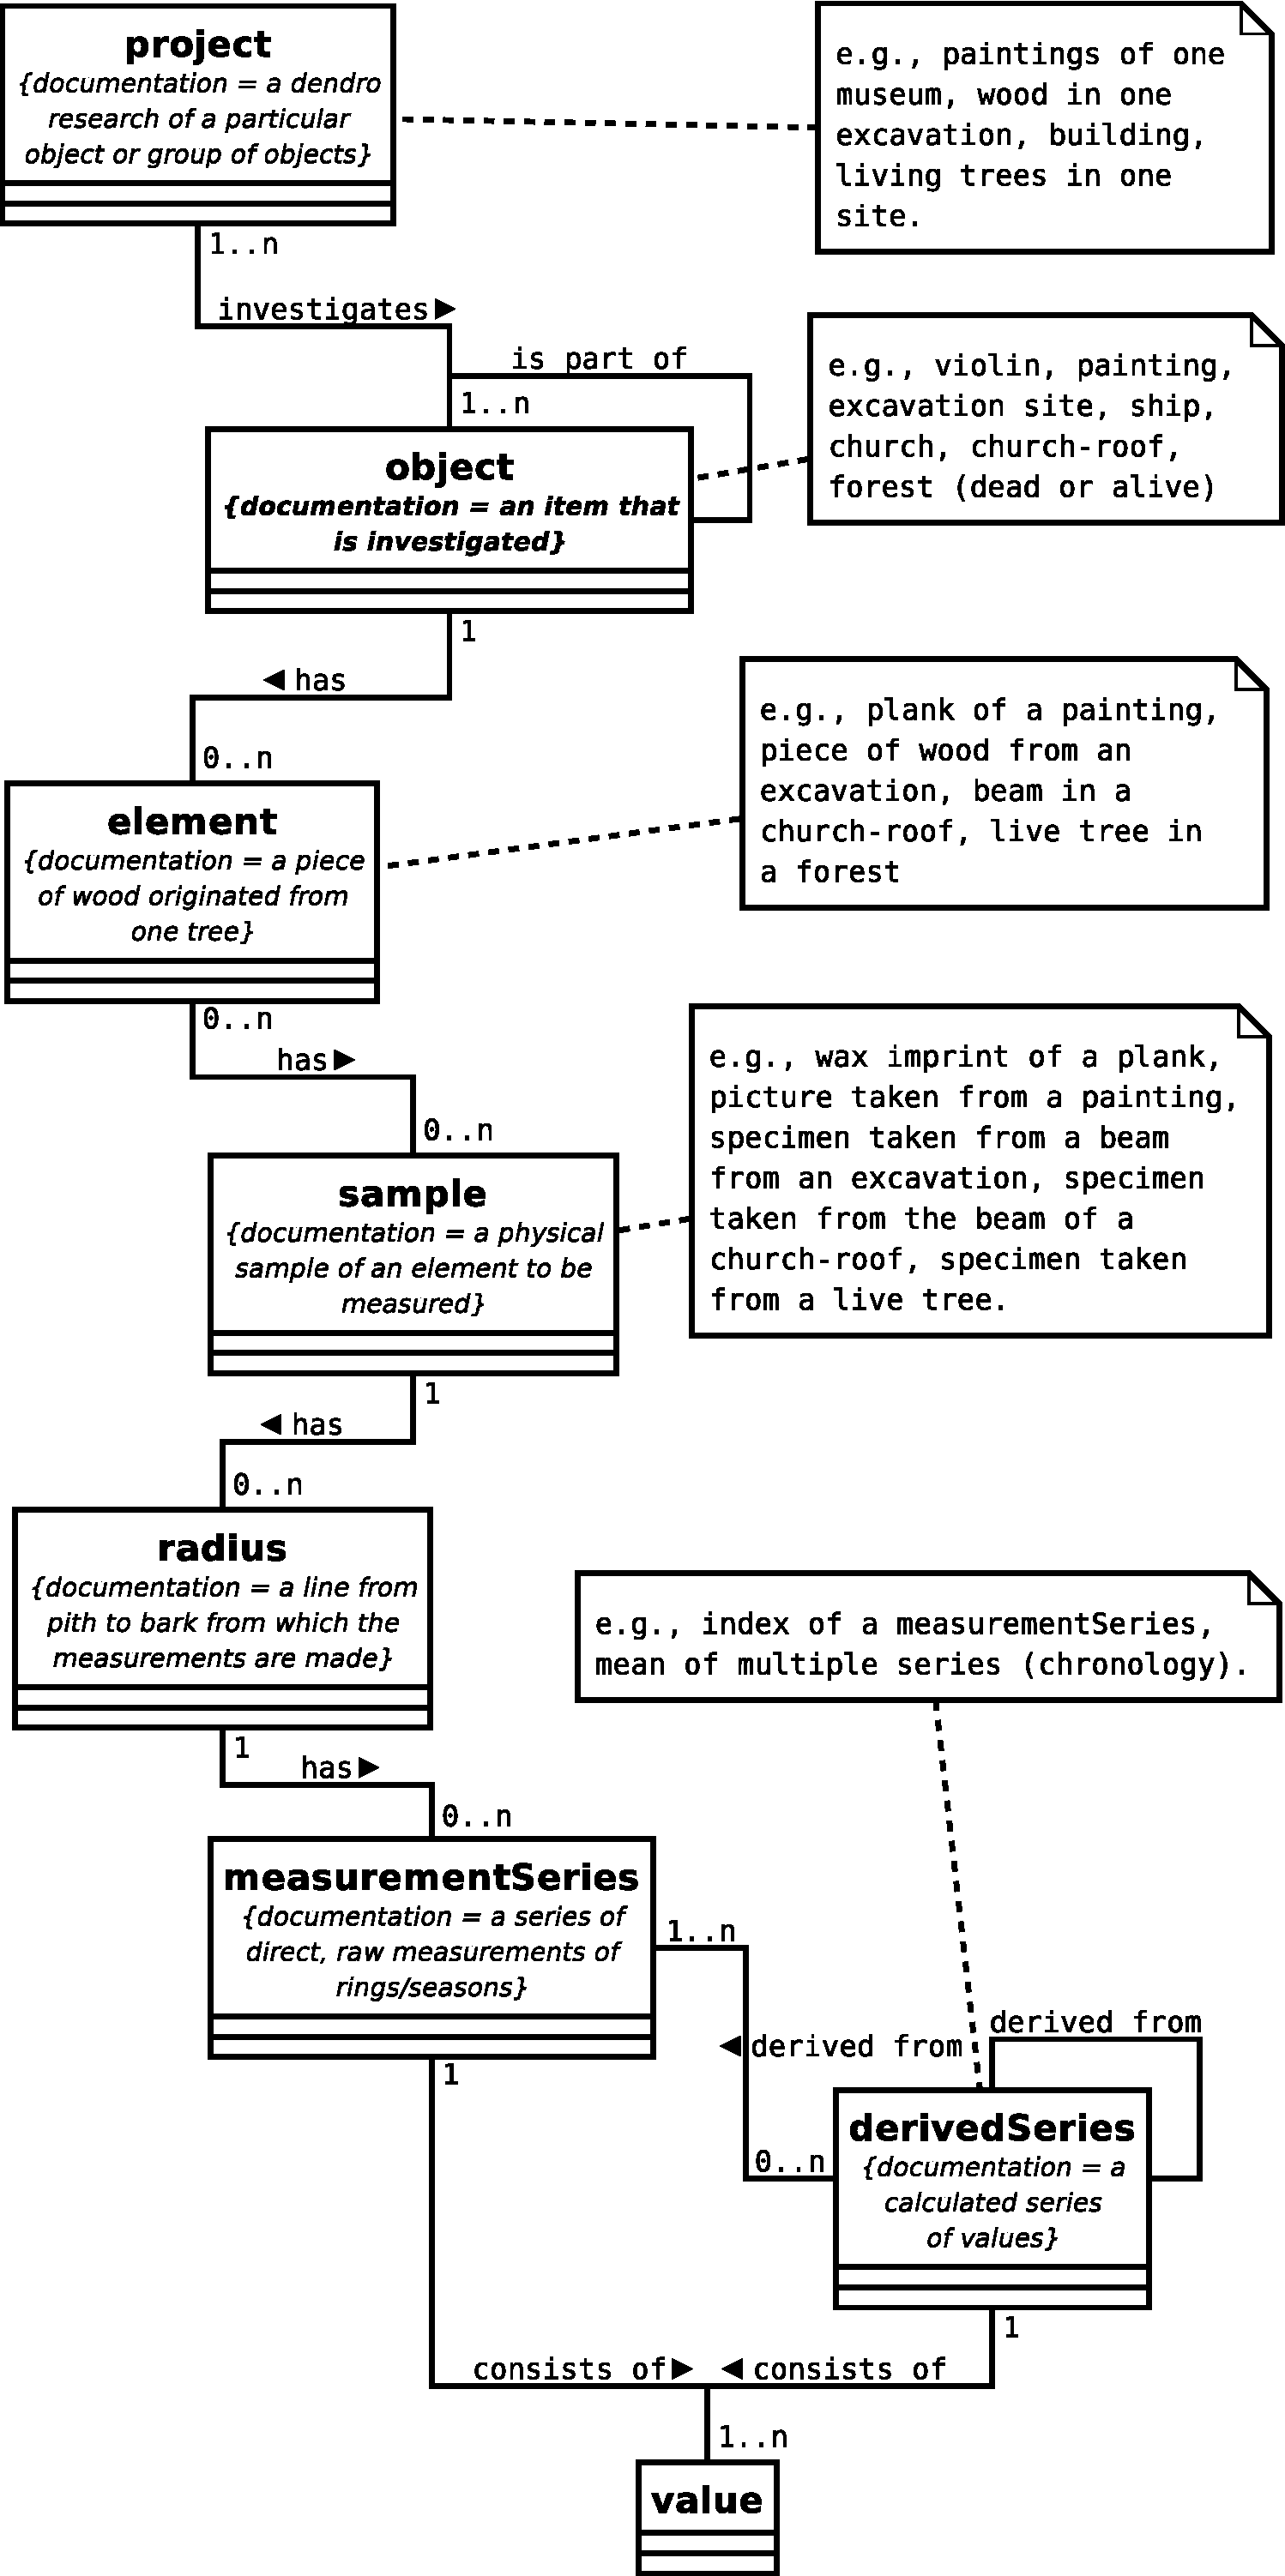
\includegraphics[height=0.9\textheight]{Images/datamodel.pdf}
\caption{TRiDaS data model showing the relationships between data entities.  Most of the entities having a simple hierarchical relationship (a project has one or more objects, an element has one or more samples.} 
\label{fig:datamodel}
\end{figure}

\begin{description}

\item 
\includegraphics[width=5mm]{Images/pixel.png}  \textbf{A project} -- is defined by a laboratory and encompasses dendrochronological research of a particular object or group of objects.  Examples include: the dating of a building; the research of forest dynamics in a stand of living trees; the dating of all Rembrandt paintings in a museum. What is considered a ``project'' is up to the laboratory performing the research. It could be the dating of a group of objects, but the laboratory can also decide to define a separate project for each object. Therefore, a project can have one or more objects associated with it.  Due to historical reasons, TRiDaS projects are not currently supported within Tellervo, although future plans include adding project support.

\item 
\includegraphics[width=5mm]{Icons/128x128/object.png} \textbf{An object} -- is the item to be investigated.  Examples include: violin; excavation site; painting on a wooden panel; water well; church; carving; ship; forest. An object could also be more specific, for example: mast of a ship; roof of a church. Depending on the object type various descriptions are made possible. An object can have one or more elements and can also refer to another (sub) object.  For instance a single file may contain three objects: an archaeological site object, within which there is a building object, within which there is a beam object.  The list of possible object types is extensible and is thus flexible enough to incorporate the diversity of data required by the dendro community.  Only information that is essential for dendrochronological research is recorded here. Other related data may be provided in the form of a link to an external database such as a museum catalogue. 

\item 
\includegraphics[width=5mm]{Icons/48x48/element.png} \textbf{An element} -- is a piece of wood originating from a single tree. Examples include: one plank of a water well; a single wooden panel in a painting; the left-hand back plate of a violin; one beam in a roof; a tree trunk preserved in the soil; a living tree. The element is a specific part of exactly one object or sub object.  An object will often consist of more than one element, e.g., when dealing with the staves (elements) of a barrel (object).  One or more samples can be taken from an element and an element may be dated using one or more derivedSeries.

\item 
\includegraphics[width=5mm]{Icons/48x48/sample.png} \textbf{A sample} -- is a physical specimen or non-physical representation of an element. Examples include: core from a living tree; core from a rafter in a church roof; piece of charcoal from an archaeological trench; slice from a pile used in a pile foundation; wax imprint of the outer end of a plank; photo of a back plate of a string instrument. Note that a sample always exists and that it can either be physical (e.g.\ a core) or representative (e.g.\ a picture). A sample is taken from exactly one element and can be represented by one or more radii.

\item 
\includegraphics[width=5mm]{Icons/48x48/radius.png} \textbf{A radius} --  is a line from pith to bark along which the measurements are taken. A radius is derived from exactly one sample. It can be measured more than once resulting in multiple measurementSeries.

\item 
\includegraphics[width=5mm]{Icons/48x48/measurementseries.png} \textbf{A measurementSeries} -- is a series of direct, raw measurements along a radius. A single measurementSeries can be standardised or a collection of measurementSeries can be combined into a derivedSeries.  The measurements themselves are stored separately as values.

\item 
\includegraphics[width=5mm]{Icons/48x48/derivedseries.png} \textbf{A derivedSeries} -- is a calculated series of values and is a minor modification of the ``v-series'' concept proposed by \cite{corina}.  Examples include: index; average of a collection of measurementSeries such as a chronology. A derivedSeries is derived from one or more measurementSeries and has multiple values associated with it.

\item 
\includegraphics[width=5mm]{Images/pixel.png} \textbf{A value} --  is the result of a single ring measurement. Examples include: total ring width; earlywood width; latewood width. The values are related to a measurementSeries or a derivedSeries. In case of a measurementSeries the variable and its measurement unit (e.g.\ microns, 1/100th mm etc) are recorded as well.  Tellervo supports both total ring width, and early/latewood values.  Support for other variables is planned for a future version.

\end{description}


Working top to bottom, the TRiDaS entities are nested within each other.  For instance a project contains one or more objects, which in turn contains one or more elements, and so on.  The benefit of this is that you record data once and once only.  In standard file-based dendrochronological software, when creating measurement series you are typically required to type the name of the site, the species of tree etc over and over again.  This is not only time consuming, but very error prone.  

Keeping data consistent is also difficult.  For instance, if it was determined that a tree species was identified incorrectly, in existing file-based software, the user would need to locate all data series from this tree and manally update the metdata.  This is not the case in Tellervo.  A tree is represented just once in Tellervo and samples of this tree, and the subsequent measurement series reference this one entry.  If metadata for this tree needs to be changed, the tree record is updated in just this one place.  Because the measurement series obtain this information by reference, then all associated series are automatically kept up to date.

\section{Entering sample metadata}
\index{Sample!Metadata, editing}
\index{Metadata!Editing}
The metadata for a series is viewed and edited on the `Metadata' tab of the main window such as that shown in figure \ref{fig:metadata}.  You can see the interface is organized according to the TRiDaS data model with separate tabs for object, through to series.  

\begin{figure}
\centering
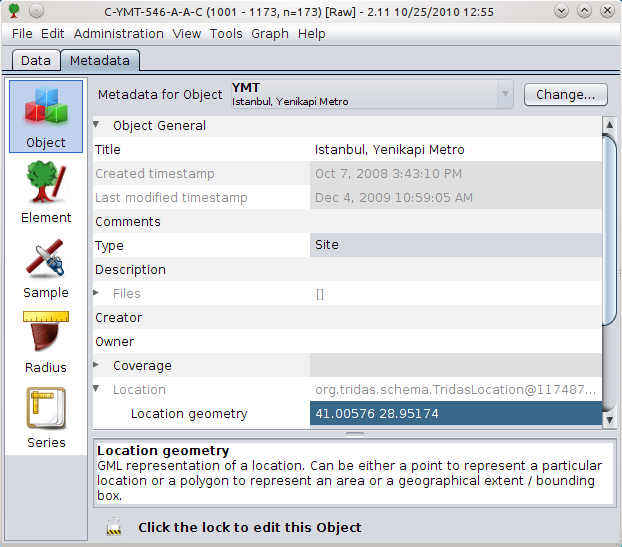
\includegraphics[width=0.6\textwidth]{Images/metadata.png}
\caption{Example of the metadata dialog.  The screen is showing the details of a TRiDaS object.  Note that the location geometry field is highlighted and so a description of what is expected in this field is given below.} 
\label{fig:metadata}
\end{figure}

When creating a new series, the metadata screens must be populated in order.  This is necessary because of the nesting of entities described above.  For instance, an element is associated with an object, so an object must be chosen before an element can be defined.  Likewise, an element must be chosen before any samples of this element can be defined.  

Much of the time the entities that you need will already be stored within the database.  Instead of re-entering data, you simply need to select the existing entry from the database, saving a great deal of time.  Depending on the situation, buttons will appear at the top of the dialog to let you `choose' an entry from the database, `revert' to the previously chosen entry, `change' the existing entry to a different one from the database, or create a `new' record.

Please note that the content of these metadata screens is kept read-only by default.  To edit the values, you must first click the padlock icon to unlock the fields.  When you have finished making changes you need to press the save button to write the changes to the database before moving to another metadata screen.

Very few of the metadata fields in the TRiDaS data model are mandatory, but a few are.  In this case, these fields are highlighted with a red star.  Note that whether a field is mandatory or not can depend on the other fields that have been filled in.  For instance, the dimensions of an element are not required, but if dimensions are given then the units for these measurements must also be provided.

A number of the metadata fields are restricted with regards the values that you can enter.  These are known as `controlled vocabularies' in TRiDaS terms.  Controlled vocabulary fields are represented by drop down menus.  Similarly fields that expect numerical values (such as element dimensions) will only allow numbers.  The final method data entry method is through custom dialogs, for example there is a custom dialog for entering location information.  This accepts coordinates in either decimal degrees or degrees minutes and seconds.  Alternatively you can use data from a GPS handset by providing a GPS Exchange (GPX) format file containing the waypoints. The GPX format is the most common interchange format for GPS data. You can pick the relevant waypoint from the drop down menu.  You can also preview the defined coordinates on a map using the `view on map' button. 

\tip{A popular open source GPS communication tool is GPS Babel.  It is an easy to use application which can download data from the majority of GPS handsets.  See \url{http://www.gpsbabel.org} for more information.}


\section{Entering bulk metadata}
\index{Metadata!Bulk entry}
\label{txt:bulkentry}
Entering metadata on a sample-by-sample basis works perfectly well, but does not necessarily fit best with the typical workflow of a laboratory.  Samples do not typically arrive in a lab in ones and twos, rather in large quantities following a field excursion.  In this case it is most efficient to enter all the metadata for the samples as they arrive.  This is often best in terms of data accuracy as the metadata can be entered while the field notes are still fresh in the mind.

To enable the efficient entry of lots of metadata Tellervo includes the bulk data entry interface.  This can be accessed from the file menu and is illustrated in figure \ref{fig:bulkentry}.  There are three pages, one each for objects, elements and samples.

\begin{figure}
\centering
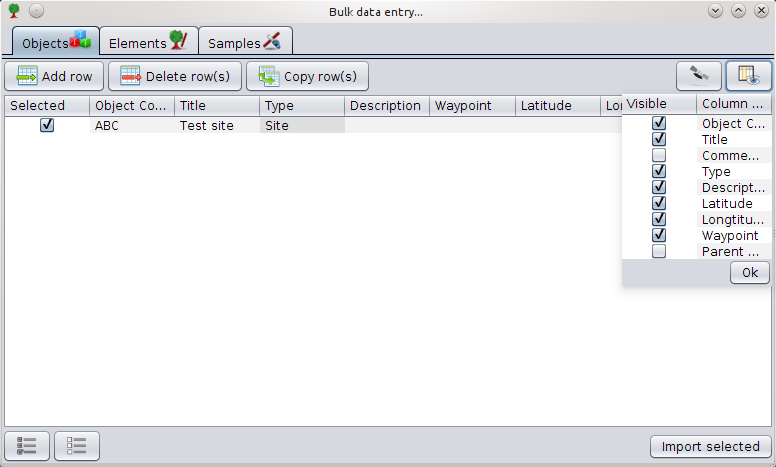
\includegraphics[width=0.6\textwidth]{Images/bulkentry.png}
\caption{The bulk metadata entry screen.  The `show/hide columns' button has been pressed showing how the user can turn on and off particular columns.} 
\label{fig:bulkentry}
\end{figure}

The interface is designed like a spreadsheet so as to be as familiar to users as possible.  Each row of the table represents a new entry in the Tellervo database.  Which columns are shown to the user is determined by the `show/hide columns' button on the top right of the screen.  

The bulk entry interface also includes support for reading GPS units.  By pressing the satellite button on the toolbar, the user can provide a GPS Exchange (GPX) format file containing the waypoint locations recorded in the field.   Tellervo will add a waypoint column to the spreadsheet with a drop down menu which will automatically populate the latitude and longitude fields for the record. 

It is common for many of the metadata fields to be the same in a single field collection.  For instance, when coring trees in a forest, they are often of the same species.  Rather than requiring the user to repeatedly type the same data over and over, the `copy row' button can be used to duplicate a record, and then the user can change the few fields that are different.

Another time saving feature is the ability to cut and paste back and forth between Tellervo and spreadsheet programs like Microsoft Excel.  This can be particularly helpful if you already have large amounts of metadata entered into a spreadsheet.  The best way to do this is to populate a row in Tellervo then copy this into Excel.  This will show then show you the order of columns and the format that Tellervo expects data to be in. 

When you have entered all the data you want, you can press the `Import selected' button to write the records to the database.  Start on the objects tab, then move to elements then samples.  

The samples page has the additional feature of creating barcode labels.  Once you've finished importing your metadata, simply press the barcode button and a PDF file will be generated.

\section{Metadata browser}
\index{Metadata!Browsing}
The metadata browser interface provides a convenient way to view all the metadata within your Tellervo database.  It can be accessed through the `Administration' menu of from the home screen.

The metadata browser contains two parts: a hierarchical representation of all TRiDaS entities in your database on the left; and a metadata viewer for the selected entry on the right.  This interface is also the best method for fixing mistakes in your database.  

Although Tellervo's database architecture maintains integrity within your data, it does come at the price of being a little more complicated to fix mislabelled series.  For instance, what if you were to measure a series 'B' and assign it to sample ABC-138-A only later to realize you misread the label and it was in fact ABC-188-A.  In a traditional file-based system, you would probably just need to rename the file you'd just created.  In Tellervo however, you need to redefine the relationship of the series within the database and reassign it to the correct sample.  This is best understood when looking at the hierarchical tree in the metadata browser.  Hopefully you will see that you what you need to do is to move the series from its current position in the database to the correct one.  

The reorganization of data in this way is achieved by right clicking on items in the hierarchical tree and choosing either `merge' or `reassign'.  These functions are only accessible to database administrators.  The reassign option simply moves an entry to a different parent in the database.  The merge tool handles the more complicated situation where a entry has been made in two different places in the database and they need to be combined.  For instance in the case described above if the erronously created ABC-138-A after (the correct) sample  ABC-188-A had already been created and populated.  In this case the `A' sample from ABC-138-A would be merged into ABC-188-A, bringing with it any radii and measurements.  Hopefully the metadata for the merged series will be identical, but in the case of discrepancies, details are noted in the comments field of the finished entity.  You should therefore take the time to check the finished entry and clarify any differences.


\section{Laboratory codes}
\index{Laboratory codes}
\index{Sample codes|see{Laboratory codes}}
Tellervo uses lab codes to refer to the hierarchical nature of the TRiDaS entities in the database.  The separate parts of the code are delimited by hyphens and depending on the level of the entity you are referring to, will have a different number of parts.  For instance, if you are referring to a tree (an `element' in TRiDaS terminology) then the lab code will consist of just two parts: the object code and the element code.  See figure \ref{fig:labcodes} for an illustrated example.

\begin{figure}
\centering
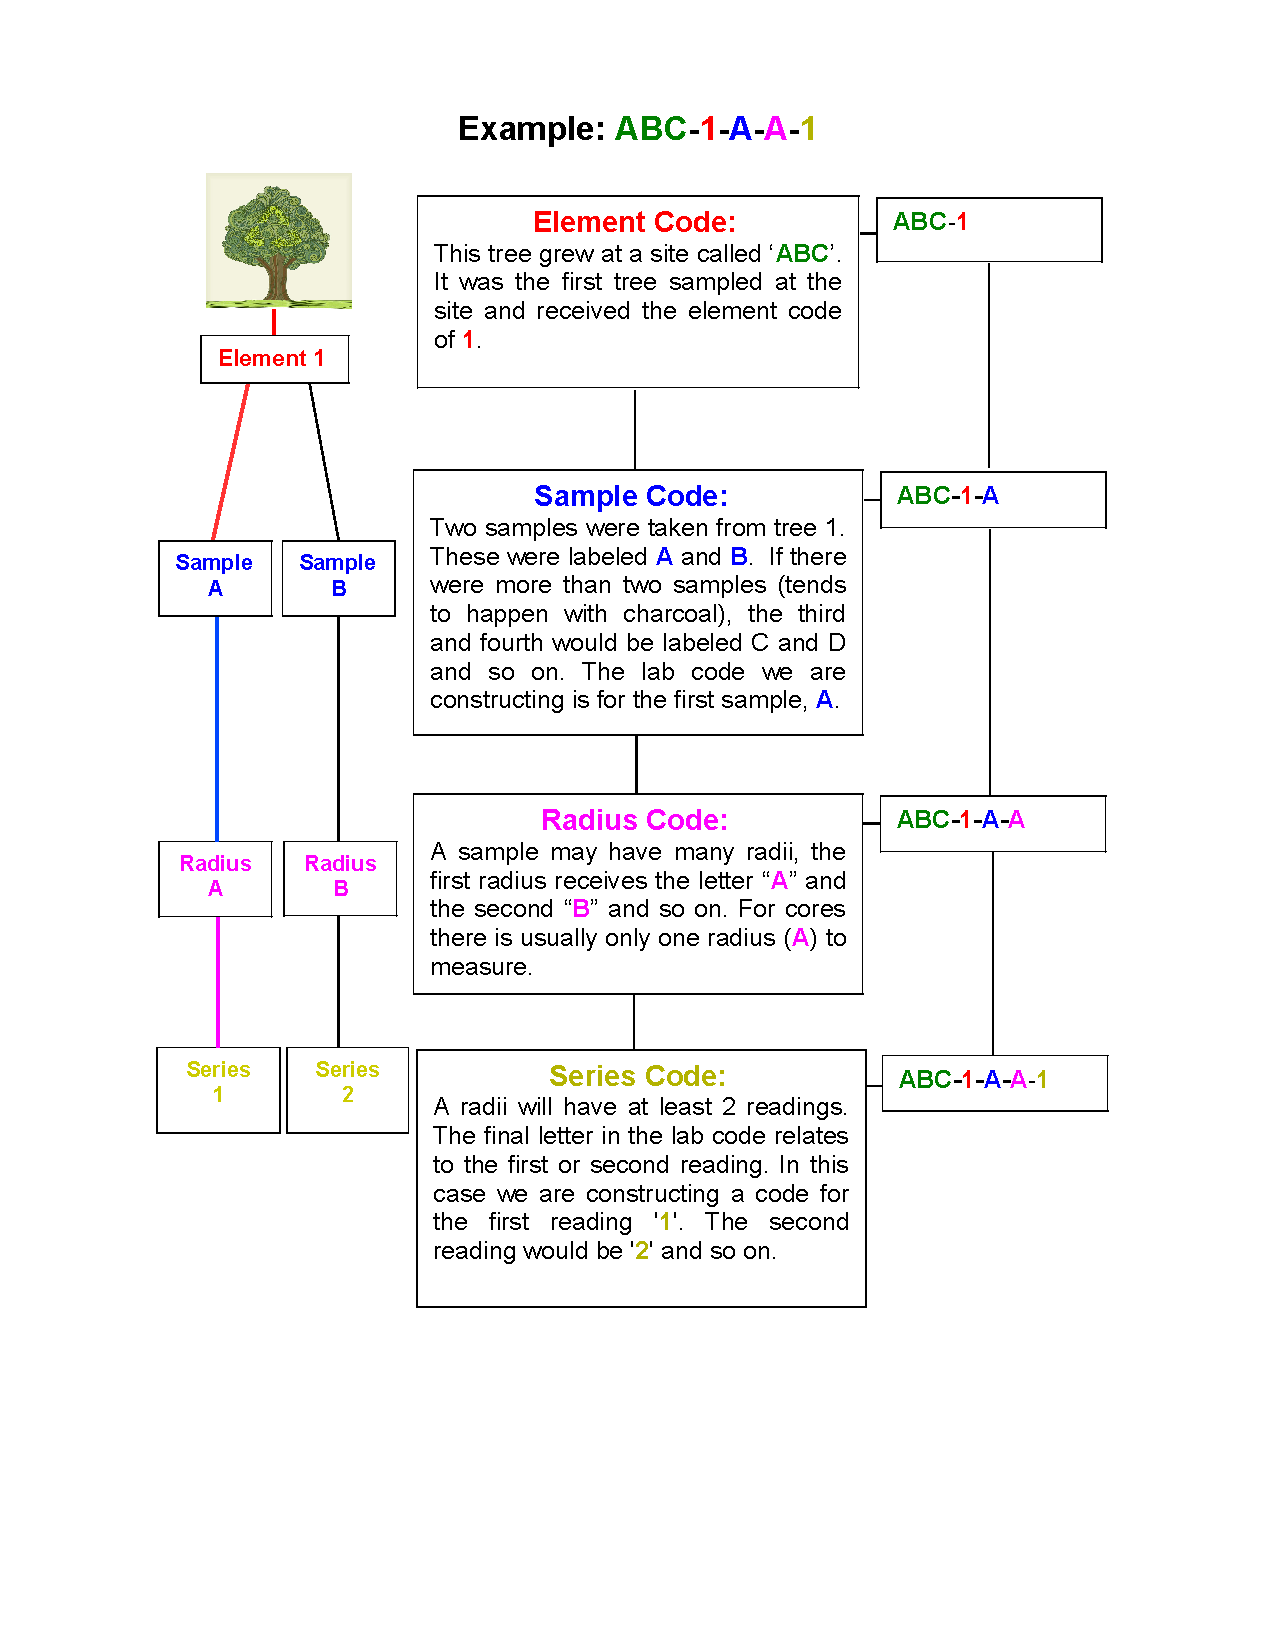
\includegraphics[trim = 1in 1.5in 1in 0.5in, clip, width=0.9\textwidth]{Images/CorinaSampleCodes.pdf}
\caption{Illustration of the how lab codes are built in Tellervo.  Figure courtesy of Charlotte Pearson.} 
\label{fig:labcodes}
\end{figure}

Lab codes are used throughout Tellervo to describe TRiDaS entities.  They can also be used in many places to specify entities that the user would like to choose.  For instance, in the database browser, you can type the lab code for an object, element, sample, radius or series to search the system for all the series that match the specified entity.  For instance entering `ABC-5' would search for all series associated with element `5' from object `ABC'.



\index{Metadata|)}



    \chapter{Mapping}
\index{Mapping|(}
Tellervo includes an integrated open source 3D mapping system (based on NASA's award winning World Wind Java SDK) similar to the program Google Earth which you're no doubt familiar with. As mentioned in the installation chapter, this mapping system requires an OpenGL 3D capable graphics card. Before you can use the mapping in Tellervo, you must also have something to map! See the chapter on Metadata (page \pageref{txt:metadata}) for information about adding coordinates to your system.

There are two ways to map data from your database. First of all, you can see a map of all the sites (i.e. TRiDaS objects) by going to \menutwo{Administration}{Site map}. This will give you a screen like this:

\begin{figure}[hbtp]
  \label{fig:map}
  \centering
  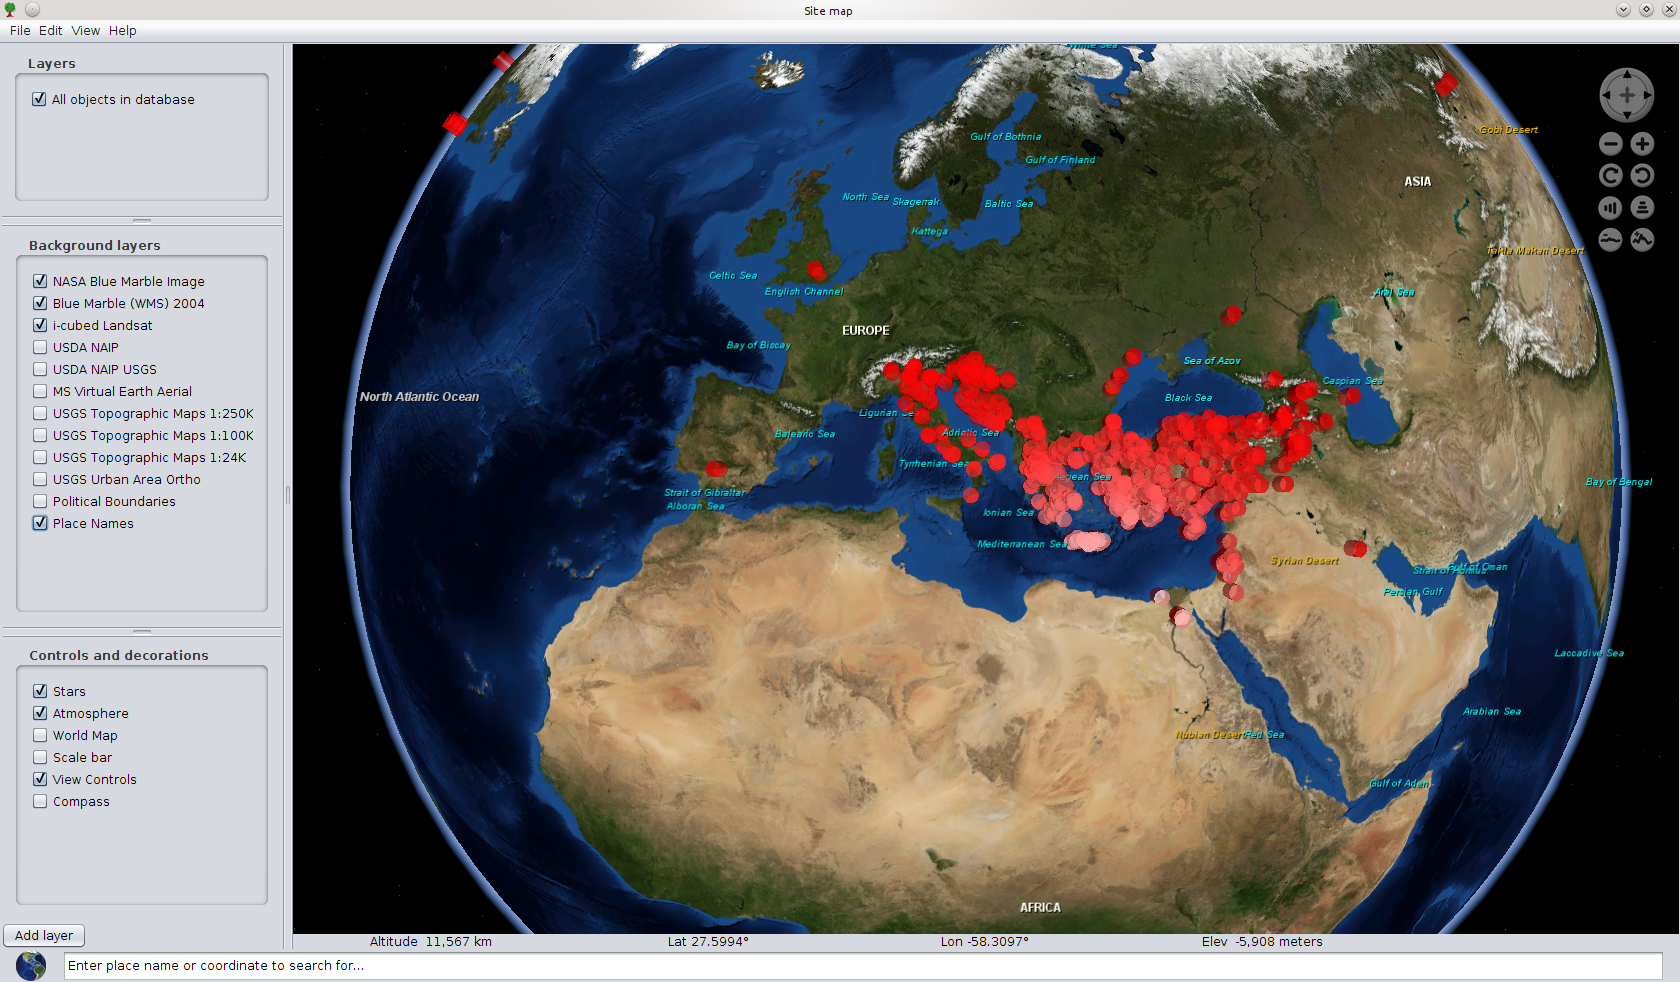
\includegraphics[width=\textwidth]{Images/sitemap.png}
  \caption{Screenshot showing an example of a site map.}
\end{figure}


You can also see a map of your current series if you have latitude/longitude metadata by clicking on the map tab on the main data screen.  
\newpage

\section{Navigation}
\index{Mapping!Navigation}
\begin{figure}[hbtp]
  \centering
  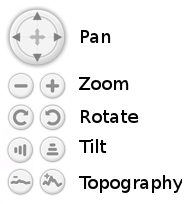
\includegraphics[width=0.2\textwidth]{Images/wwjcontrols.png}
  \caption{On-screen navigation controls.}
  \label{fig:wwjcontrols}
\end{figure}

You can navigate around your maps using the on screen controls (figure \ref{fig:wwjcontrols}), by using your mouse and/or your keyboard.  These controls enable you to explore your location information in 3D such as the example of Mount Vesuvius in figure \ref{fig:mappin}.




\subsection{Mouse with scroll wheel}

\begin{description*}
      \item[Pan] Left mouse button click and drag -- all directions
      \item[Zoom] Use the scroll wheel on the mouse or Left and Right mouse (both buttons) click and drag up and down
      \item[Tilt] Right mouse button click and drag -- up and down or use `Page Up' and `Page Down' on the keyboard.
      \item[Rotate] Right mouse button click and drag -- left and right Note: Crossing the top and bottom half of the screen while rotating will change direction.
      \item[Stop] Spacebar
      \item[Reset Heading] N
      \item[Reset all] R 
\end{description*}



\subsection{Single button mouse}
\begin{description*}
     \item[Pan] Left mouse button click and drag - all directions. L left mouse button click once to center view.
     \item[Zoom] Hold `Ctrl' on the keyboard and Left mouse button click and drag - up and down
     \item[Tilt] Hold `Shift' on the keyboard and Left mouse button click and drag - up and down or use "Page Up" and "Page Down" on the keyboard.
     \item[Rotate] Hold `Shift' on the keyboard and Left mouse button click and drag - left and right
     \item[Stop] Spacebar
     \item[Reset Heading] N
     \item[Reset all] R 
\end{description*}

%\begin{SCfigure}
%  \centering
%  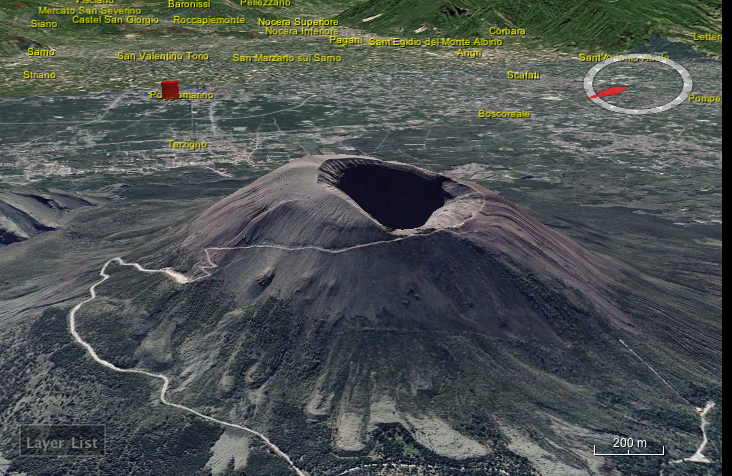
\includegraphics[width=0.8\textwidth]{Images/3dmapexample.png}
%  \caption{Example of 3D mapping in Tellervo.}
%  \label{fig:3dmap}
%\end{SCfigure}

Another method of navigating around the map is by using the built in gazetteer. You can enter and place name or coordinate information into the box at the bottom of the screen and you will fly to the requested location. 


\section{Interacting with data}

Each marker on the map represents either a TRiDaS object or element in your Tellervo database. By clicking on these pins you can get more information from the database (see figure \ref{fig:mappin}).

\begin{figure}[hbtp]
  \centering
  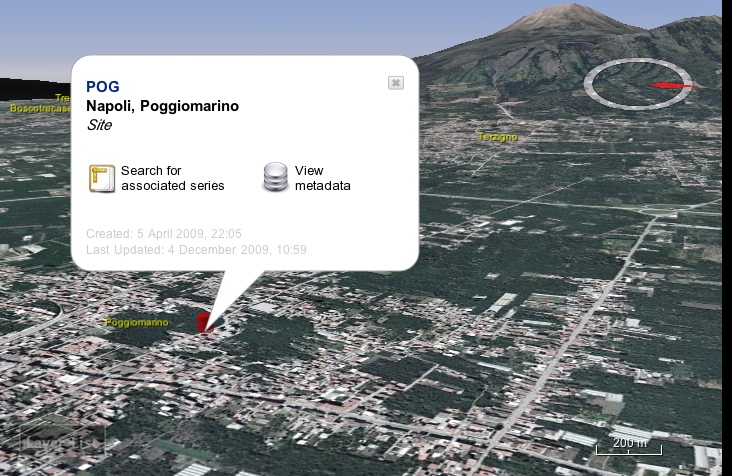
\includegraphics[width=0.8\textwidth]{Images/mappinexample.png}
  \caption{Screenshot of a map with information pin expanded}
  \label{fig:mappin}
\end{figure}

The example above shows the ring marker is of a site in Napoli called Poggiomarino (code name POG). You can see the option for searching for all series in the database associated with this site, and also the option for viewing all the metadata. 

\section{Map layers}
\label{txt:userAddWMS}
\index{Mapping!Layers}

Tellervo comes ready configured with basic map layers, including high resolution satellite imagery and basic political features. You can turn background layers on and off by going to \menutwo{View}{Layers} or using the layer panel at the left of the screen when using `Site map'.

Map layers are downloaded on-the-fly so there is likely to be a delay when you initially visit to a new region. However, up to 2Gb of map data can be cache locally to your hard disk, so on future visits, maps should load quickly.

\subsection{Data layers}
Data map layers (i.e.\ site and sample locations) are controlled with the layer list on the left of the screen. When viewing series, you will have the option of adding layers containing points for all the other series at the current site, and showing all the sites in the database. 

In the `Site map' you can use the `Add layer' button to add data layers of the following types:

\begin{description}
 \item[All Tellervo objects] -- this adds a single layer containing all the objects within the Tellervo database.
 \item[Tellervo entity from database] -- this adds a layer containing the location of one record from the Tellervo database.  This is specified by labcode e.g. ABC would add a pin for the site ABC, whereas ABC-1 would add a pin for the element ABC-1.
 \item[Elements from an object] -- this adds a layer containing all the elements for a specified object.  The object is specified by labcode.
 \item[All ITRDB sites] -- this downloads the location of all sites currently available in the ITRDB database and adds them as a single layer.
 \item[ESRI Shapefile] -- this enables you to load an ESRI shapefile stored locally on your computer.  Tellervo supports polygon, polyline and point files, although currently it does not enable you to style this data.  Data for a layer is presented using a random color.
 \item[Google Earth KML/KMZ file] -- like the ESRI shapefile option this enables you to load spatial data from your computer.
 \end{description}


\subsection{Web Map Service (WMS)}
\index{Web Map Service (WMS)}
\index{Mapping!Web Map Service (WMS)}

The mapping system in Tellervo includes support for remote map servers that use the OGC Web Mapping Service (WMS) standard. If you go to \menuthree{View}{Layers}{Add remote layers}, you will get a dialog with a tab for each WMS server configured for your system. By default this includes the NASA Earth Observation and Jet Propulsion Lab servers.  By ticking layers in this list you can add data layers to your map.

You can add map data from other WMS servers by clicking the `+' tab and entering the URL of the server you would like to use.  This will give an additional tab with all the available map layers.  This server will only be available for the duration of your current session so will need to be added each time you start Tellervo.  If you would like a particular WMS server to be made permanently available, your Tellervo administrator can do this (see `Managing map services', on page \pageref{txt:managingmaps} for further details).  Additional WMS servers added in this way will be available to all users the next time they connect to your Tellervo server.

Your system administrator may host a map server specifically for your lab, for instance, containing high resolution plans of an archaeological site that you are working on, or environmental data for your study region. Figure \ref{fig:wms} shows an example overlay of sea surfaces temperatures loaded dynamically from the NASA EO server.

\begin{figure}[hbtp]
  \centering
  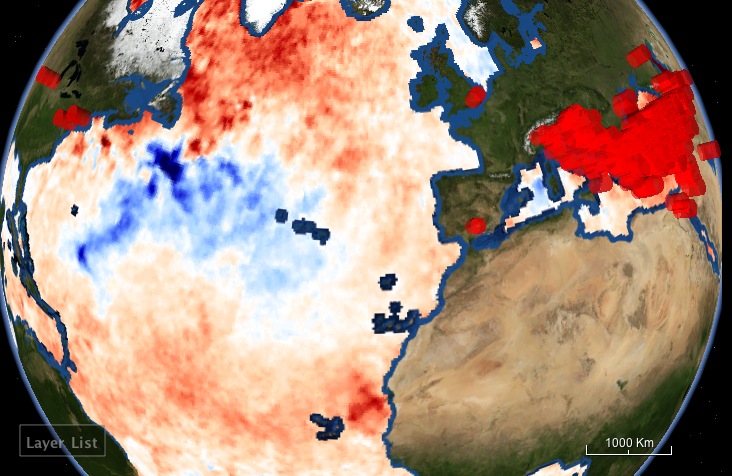
\includegraphics[width=0.8\textwidth]{Images/sst.png}
  \caption{Map screenshot with a NASA sea surface temperature overlay dynamically loaded from the NASA WMS server.}
  \label{fig:wms}
\end{figure}





\section{Exporting maps}
\index{Export!Maps}
You can export maps by going to \menutwo{File}{Export map as image}. For best results, maximize your map window first. You may also like to turn off various map widgets by going to the View menu. The exported image will include everything you can see on your map screen. 


\index{Mapping|)}
    \chapter{Graphing}

The graphing component is reused in many places throughout the Tellervo desktop application.  The following description although based on the main graphing screen in Tellervo is largely applicable to all dialogs that include graphs (e.g.\ crossdating, indexing and reconciliation).  

The main method for graphing your tree-ring data is by choosing an option from the Graph menu.  Depending on the type of series you have open, the options available to you will be different.  For raw measurement series, you will just have the option to `Graph active series'.  This will give you a simple graph of the current series that you have open.  If you have a derived series open, then you may also choose `Graph component series' which will plot all the series that go to create this series, or 'Graph all series' which graphs all the component series as well as the current series.

\section{Controlling graphs}

When newly created graphs are plotted according to the scale on the axes.  A feature of Tellervo graphs though is that they can be manipulated directly on the screen.  Both dendrochronology was computerized, dendrochronologists would plot rings manually on to graph paper.  These paper graphs were then placed on lightboxes and moved around to enable comparisons.  The graph function in Tellervo emulates this behaviour allowing users to click and drag graphs around to test for visual matches.

Figure \ref{fig:graph} shows an example graph dialog.  The mouse is hovering of the blue measurement series at relative year 1040 illustrating Tellervo's highlighting and guide line capabilities.  A feature not shown in this screenshot is the illustration of sapwood rings.  When sapwood rings are present the corresponding years on the chart are denoted via a heavier line.

\begin{SCfigure}
  \centering
    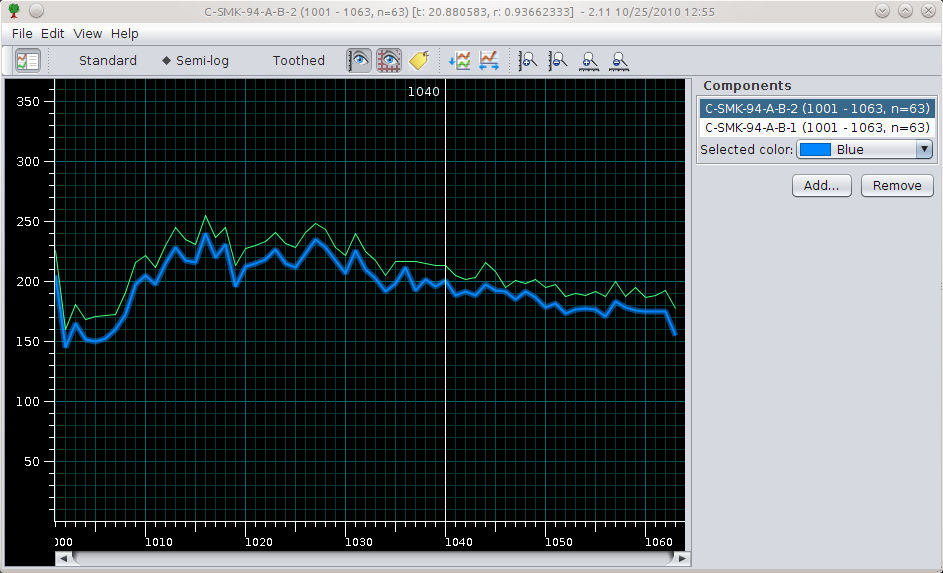
\includegraphics[width=0.6\textwidth]{Images/graph.png}
    \caption{An example graph window containing two undated series of the same sample on a semi-log graph.  Note the legend is visible with the options for adding or removing series.}
    \label{fig:graph}
\end{SCfigure}


The layout of graphs can be changed using both the toolbar buttons and menu options.  The type of graph can be changed between a standard line graph, a semi-log graph and a toothed graph using the radio buttons.  The remaining buttons are as follows:

\begin{center}
\begin{tabular*}{0.8\textwidth}[h]{lp{10cm}}
 
\includegraphics[width=4mm]{Icons/22x22/haxiszoomin.png} & Zoom in on the horizontal axis \\
 
\includegraphics[width=4mm]{Icons/22x22/haxiszoomout.png} & Zoom out on the horizontal axis \\
 
\includegraphics[width=4mm]{Icons/22x22/vaxiszoomin.png} & Zoom in on the vertical axis \\
 
\includegraphics[width=4mm]{Icons/22x22/vaxiszoomout.png} & Zoom out on the vertical axis \\
 
\includegraphics[width=4mm]{Icons/22x22/showgrid.png} & Toggle show/hide the grid lines \\
 
\includegraphics[width=4mm]{Icons/22x22/label.png} & Toggle show/hide the series labels \\
 
\includegraphics[width=4mm]{Icons/22x22/vaxisshow.png} & Toggle show/hide the vertical axis \\
 
\includegraphics[width=4mm]{Icons/22x22/spreadvertically.png} & Spread the series evening up the vertical axis \\
 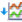
\includegraphics[width=4mm]{Icons/22x22/squeezevertically.png} & Set the baselines of all the series to zero \\
 
\includegraphics[width=4mm]{Icons/22x22/fitcharthoriz.png} & Resize graph to fit horizontally \\
 
\includegraphics[width=4mm]{Icons/22x22/legend.png} & Toggle show/hide the legend\\
\end{tabular*}
\end{center}

There are also a number of keyboard shortcuts that you might find useful:

\begin{description*}
 \item[Tab] : Cycles through each graph component
 \item[Ctrl+W] : Increase vertical scale
 \item[Ctrl+S] : Decrease vertical scale
 \item[Ctrl+A] : Increase horizontal scale
 \item[Ctrl+D] : Decrease horizontal scale
 \item[Up arrow] : Moves selected graph up by 10 units
 \item[Down arrow] : Moves selected graph down by 10 units
 \item[+] : Moves selected graph up by 1 unit
 \item[-] : Moves selected graph down by 1 unit
 \item[HOME] : Scroll to first year of series
 \item[END] : Scroll to last year of series
 \item[PAGE UP] : Scroll left by one page width
 \item[PAGE DOWN] : Scroll right by one page width
 \item[SPACE] : Sets horizontal origin of all graphs to the same value 
\end{description*}

\section{Exporting graphs}

To export your graphs for use in reports you can go to \menutwo{File}{Export plot as PDF file}, or \menutwo{File}{Export plot as PNG file}.  This presents you with a dialog for setting the colors, labels and size of the exported image.  This functionality is due for an overhaul in the future to provide more flexible support for publication quality graphics.  

    \chapter{Importing and exporting}
\label{txt:importExport}
Importing and exporting of dendro data in Tellervo is provided through the TRiCYCLE libraries.  TRiCYCLE is a universal dendro data conversion application for converting back and forth between 24 supported data formats \citep{tricycle}.  The open source libraries that provide the functionality to TRiCYCLE are incorporated directly into Tellervo providing support for all these formats.  

\begin{table*}[htbp]
\centering
\label{txt:formatList}
\index{File formats}
\begin{tabular*}{0.8\textwidth}{ll}
\toprule
Belfast Apple & Nottingham \\
Belfast Archive & ODF Spreadsheet \\
Besancon (including SYLPHE variants) &   Oxford\\
CATRAS & PAST4\\
Cracow Binary Format & Sheffield D-Format (Dendro for Windows)\\
Comma delimited text files (CSV) &  Topham \\
Corina Legacy &  TRiDaS\\
DendroDB & TRIMS\\
Heidelberg (TSAP-Win) &  Tucson (RWL and CRN)\\
KINSYS-KS & Tucson Compact\\
Microsoft Excel 97/2000/XP & VFormat \\
Microsoft Excel 2007 & WinDENDRO\\
\bottomrule
\end{tabular*}
\caption{List of the twenty-four formats supported by Tellervo. See appendices \ref{txt:fileFormatsStart}--\ref{txt:fileFormatsLast} (pages \pageref{txt:fileFormatsStart}--\pageref{txt:fileFormatsEnd}) for full descriptions.}
\end{table*}



\section{Exporting data}
\index{Export!Data}
Exporting data is initiated by the \menutwo{File}{Export data menu}.  If this is called from the main Tellervo data window, it will export the current series.  If it is called from the Tellervo home screen, then it will present you with the database browser and allow you to pick one or more series to export.  If you use the menu from within the main data editor then it will export 

\begin{SCfigure}
  \centering
    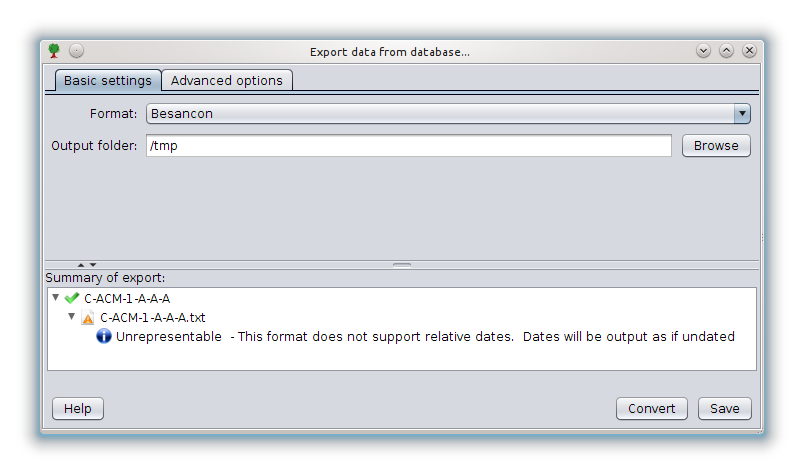
\includegraphics[width=0.7\textwidth]{Images/exportdata1.png}
    \caption{Screen showing a series that has been exported to Besan\c{c}on format.  In the summary of the export at the bottom of the screen you can see the warning to the user that this format does not have the ability to represent relative dates properly.}
    \label{fig:exportdata}
\end{SCfigure}

The export dialog contains two tabs.  The first allows the user to choose the format that they would like to export to and the folder into which to save the result.  Note that the user needs to specify a folder not a filename as many formats are unable to store more than one series in a file.  When exporting derived series such as chronologies, the export dialog may therefore need to create multiple files.  The second tab contains advanced options for altering the behaviour of the exporter:

\begin{description}
 \item[What to export] -- This option enables the user to choose between exporting just the current series, or the current series and all associated series
 \item[Grouping]  -- This enables the user to choose to group files into a single export file if possible.  For formats that do not support more than one series in a file, this option is ignored.
 \item[Naming] -- This configures how the output files are named.  See section \ref{txt:namingConventions} for more details.
 \item[Encoding] -- This specified the character encoding to use in the exported text file. See section \ref{txt:characterSets} for more information. 
\end{description}

\subsection{Naming conventions}
\label{txt:namingConventions}
\index{Naming conventions}
The naming convention is used to determine how to name the output files. The naming convention
relates to the filename itself and not the file extension. The file extension is specific to the output format
chosen (e.g. Heidelberg files are .fh and TRiDaS files are .xml).

\begin{description}
 \item[Numerical] -- This is the default naming convention. It uses the name of the input data file and
appends an incrementing number if more than one output file is produced.
 \item[UUID] -- This gives all output files a random named based on Universally Unique Identifiers
(UUIDs). This is a 36 character hexadecimal code which due to the astronomically
large number of possible combinations is guaranteed to be universally unique. A
typical filename will look like: 550e8400-e29b-41d4-a716-446655440000.
 \item[Hierarchical] -- This uses the hierarchical structure of the TRiDaS data model to provide a meaningful
name for the output file. It joins together the title of each entity in the file beginning
with the project name through to the series name. For files that contain multiple series,
the name will contain details of all the entities shared by all the series in the file. For
example, if a file contains several series from the same sample, then the file name
will be projectTitle-objectTitle-elementTitle-sampleTitle. If the file contains several
series from different samples of the same object, then the file would be projectTitle-
objectTitle. If multiple output files end up with the same name then like the numerical
convention described above, the files will have an incremental number appended to
the end. Unfortunately, most input data files do not contain rich name information
so files end up being called unnamedProject-unnamedObject-unnamedElement etc.
This convention is therefore more appropriate when converting from TRiDaS to other
formats.
\item[Series code] -- This convention is only applicable to formats that contain just one series.  The file is named according to the series code.
\item[Series code (8 characters)] -- Same as `Series code', however the file name is truncated to 8 characters if the series code is longer.  
\item[Keycode] -- Similar to `Series code' but preferentially uses a keycode (supplied by some file formats) if available.  If a keycode is not provided, then it falls back to using the series code.
 \end{description}

Note that some formats (e.g. CATRAS) require the file name to be the same as a field within the file.  In this case the naming convention is overidden, so no matter what convention you specify the filename will be the same.  If you manually rename a CATRAS file you will come across errors when loading it in the CATRAS application.

\subsection{Character sets}
\label{txt:characterSets}
\index{Character sets}
\index{Encoding}
Character sets are the
mechanism for pairing computer character codes with the character glyphs that we read. The widely
used standard was originally ASCII, but this does not include diacritic characters, and characters specific
to certain languages. There have since been many character encodings proposed (e.g ISO 8859-1 for
Western Europe and ISO 8859-7 for Greece) as well as some that are specific to Windows and Mac
operating systems (e.g. Windows-1252 and MacRoman). The character set that is becoming most widely
used today is Unicode UTF-8. This is capable of representing the vast majority of characters (107,000+) while remaining
backwards compatible for the 128 characters that ASCII is able to represent.

If an incorrect character encoding is used to interpret a file, normally the majority of characters will display
correctly (where the character sets share the same encodings) but more unusual characters will be displayed
incorrectly - typically square boxes or question marks.

The character encoding is set to the default for the operating system you are running. For instance on
MacOSX this will be MacRoman and for Windows it will be Windows-1250. If you know your input file
is in a different encoding you should set it in the input charset box. If your output file needs to be read
on an operating system other than the one you are currently running, then you may like to override the
writer charset. Please note that for certain writers, the character set used is part of the file specification
(e.g. TRiDaS must be UTF-8). In this case your choice will be ignored.

The final complication with regards character sets is the line feed character(s). For historical reasons
different operating systems use different characters to represent a new line. Depending on the software
that is used to read a file, this can cause problems. Tellervo itself will automatically adapt to files with
any type of line feed characters so reading files in Tellervo will never be a problem. When writing
out files, Tellervo will use the default line feed for the operating system you are running, unless you
choose a platform specific character set. For instance if you run Tellervo on Windows and choose a
MacRoman writing charset, Tellervo will use Mac style line feeds.

\section{Importing data}
\index{Import}
The first and simplest method for importing existing data into Tellervo is using the simple \menutwo{File}{Import data} menu.  This allows you to read in the raw ring width data values from existing files without taking any notice of associated metadata.  This option is suitable if the format you are importing is a data-only format, or if the file doesn't contain a meaningful amount of metadata.

\warn{The Tellervo system is currently limited to reading in raw data files.  It does not allow for reading in of chronology files as these contain a more complex level of metadata.  Support for chronology files will be included in a later release.}

Import the data by going to \menutwo{File}{Import data} and then choose the format that your file is in.  If you are unsure, you can use appendices \ref{txt:fileFormatsStart}--\ref{txt:fileFormatsLast} (pages \pageref{txt:fileFormatsStart}--\pageref{txt:fileFormatsEnd}) to help you.  You may also like to download TRiCYCLE\footnote{TRiCYCLE is available from \url{http://www.tridas.org/tricycle}} which includes a file identification tool in the help menu.

If your file does not explicity indicate what units the measurements are in, a dialog box will ask you to specify.  Once you have done this, a standard data editor window will appear with your data in it.  If the file you import contains multiple series, you will have a separate windows for each series.  If you then go to the metadata tab you will notice that none of the metadata have been set.  Before you can save to the database, you will need to sequentially go through the object, element, sample, radius and series tabs and either choose an existing entry from the database, or create a new record if the particular entry is not already represented.  


\section{Importing data and metadata}
\index{Import}

The second import method in Tellervo imports both data and metadata into the Tellervo database.  Unfortunately, this is an unavoidably long-winded task.  For dendro applications that do not manage the underlying data and metadata, the task of opening up legacy data files is much simpler.  In Tellervo, however, we are more fastidious about our information.  Importing legacy data files is not just a matter of reading the ring width values, but also interpreting the metadata so that it is standardized, clean and matches our high data integrity standards.  As you can imagine, this comes at the price, although definitely a price worth paying!  Before continuing, you need to have a basic understanding of the TRiDaS data model.  See chapter \ref{txt:metadata} (page \pageref{txt:metadata}) for more information.




\subsection{The import dialog}
You can launch the import dialog by going to \menutwo{File}{Import data and metadata} and then choosing the format that your file is in. 

\begin{figure}[htbp]
  \centering
    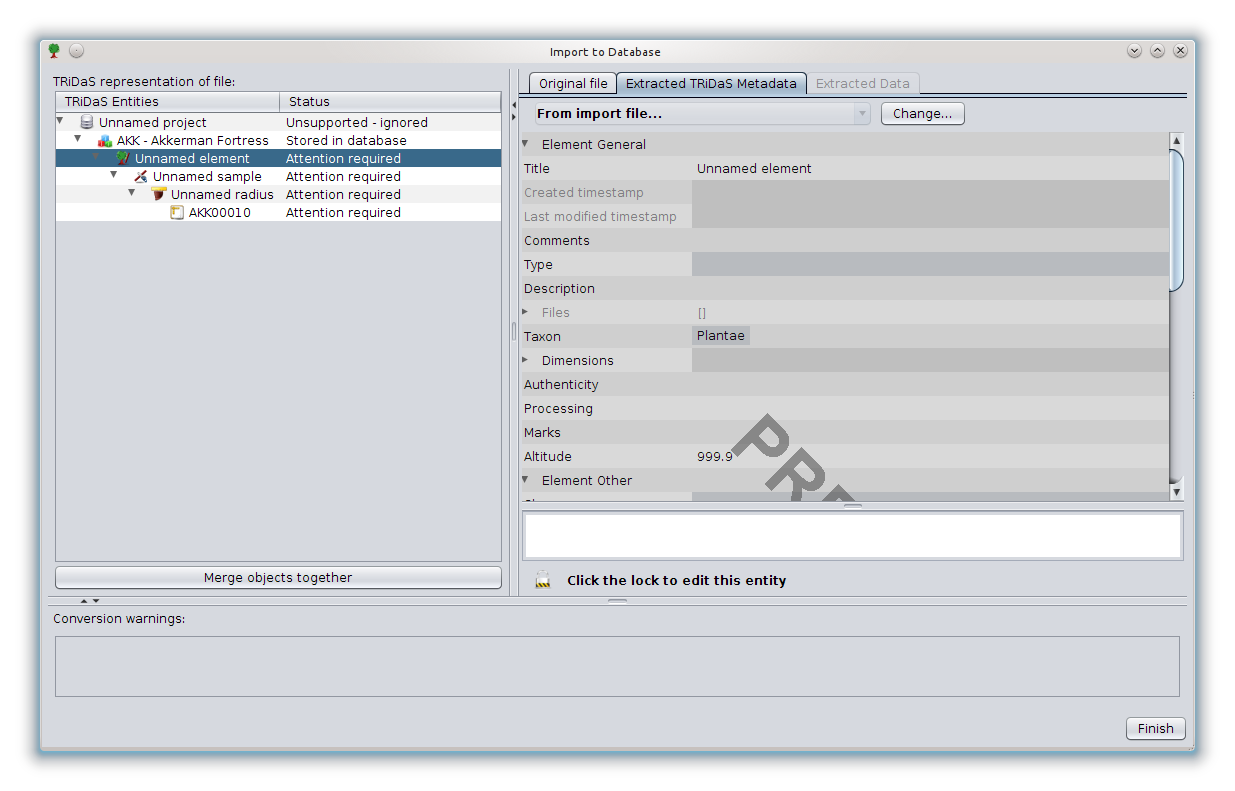
\includegraphics[width=0.95\textwidth]{Images/importdata1.png}
    \caption{Screenshot of the import dialog.  The screen is divided into three main sections.  The top left contains a TRiDaS representation of the data file that is being imported.  The top right panel contains the metadata gleaned from each of these TRiDaS entities.  At the bottom of the screen is a table containing any warnings associated with the conversion.  In this case there are no warnings. }
    \label{fig:import}
\end{figure}

Once you have picked the file you'd like to import, an import dialog screen similar to that shown in figure \ref{fig:import} is displayed. The dialog is divided into three main sections: TRiDaS hierarchy (top left); Data viewer (top right); and Warnings panel (bottom).   

The TRiDaS hierarchy panel contains a representation of the file being imported according to the TRiDaS data model.  This table also contains a status column to indicate whether input is required from the user.  The two main status options are `Stored in database'--to indicate that the entity is already stored in the Tellervo database--and `Attention required'--to indicate the entity needs to be cleaned up by the user.  

The data viewer panel on the top right of the dialog contains three tabs.  The first gives a standard text editor representation of the file being imported.  Note that when errors are detected in the file, Tellervo will highlight, where possible, the portion of the file that is causing the problem.  The second tab contains a metadata editor for the current TRiDaS entity.  The third tab contains a viewer for ring width values if the entity selected is a measurment series.

The warnings panel at the bottom of the screen contains a list of any warnings that have occurred during the conversion process.  There can be many issues when reading legacy data files, for instance some files do not contain information on the measurement units used.  In this case Tellervo will make an assumption and warn the user.  It is important to understand the assumptions and warnings provided by Tellervo in this panel otherwise erroneous (meta)data may be imported.

\subsection{Importing when entities are already in the database}
If you already have the object, element, sample and radius entities entered in your Tellervo database for the series you are trying to import the import process largely involves picking the relevant entities from the database.  

First of all, click the most senior entity in the TRiDaS hierarchy on the left which has the status `Attention required'.  The dialog will update and the limited metadata that Tellervo has been able to glean from the file will be shown on the right.  As we already have all the information we need about this entity stored in the database, we simply need to replace this `skinny' entity with the rich one we have in the database.  This is down by clicking the `Change' button in the metadata viewer on the right and then by choosing the correct entity from the pull down menu.  Click the choose button and the swap will be complete.  Notice now that in the TRiDaS hierarchy that the status for this entity is changed to `Stored in database'.  You can continue working down the hierarchy in a similar way.

\subsection{Importing when entities are not in the database}
If you are importing a file that contains entities that you \emph{don't} already have stored in your database, then you will need to clean them up and save them.   Select the most senior entity that needs to be imported in the TRiDaS hierarchy panel.  The metadata gleaned by Tellervo from the legacy file will be previewed in the metadata panel on the right.  Next, click the `lock' icon at the bottom of the metadata panel and the metadata will become editable.  You will then need to spend some time filling out and cleaning up the metadata for this entity.  

An important part of the import process is the standardization of the metadata.  Take for instance the example of the taxon.  Most legacy files have some method for indicating what species a file is about, but most do so by allowing the user to type in a free text field.  The TRiCYCLE libraries that Tellervo uses are able to read such fields but the red oak (\textit{Quercus rubra}) may be represented in many ways: oak, red oak, Oak, \textit{Quercus}, \textit{Quercus} sp., \textit{Quercus rubra}, QUER etc, not to mention the scientific synonyms for the species e.g. \textit{Quercus acerifolia}, \textit{Quercus ambigua}, \textit{Quercus angulizana} to name but a few.  Many users would know that these represent the same species, but if you were to query your database for \textit{Quercus rubra}, you would miss records stored under the other names.  It is therefore essential to standardize them to a single dictionary of terms.  In the case of species names, Tellervo use the Catalogue of Life \citep{col}.  There are a number of similar enumerated metadata fields in Tellervo, each indicated by a pull down menu.  When importing, these fields will be populated with the non-normalized term read by Tellervo, but to successfully import the entity into the database, you will need to choose the corresponding `controlled vocabulary' term from the pull down menu.  

Once you have cleaned and normalized your metadata, you need to press the `Save changes' button to upload the entity into the database.  You will be provided with an error message if you have missed any mandatory fields, or if you have not normalized all the data to terms stored in the Tellervo dictionaries.  Once you have successfully saved the entity, the TRiDaS hierarchy on the left will be updated so the status reads `Stored in database'.  You will then need to work your way through the remaining entities to finish importing the file.

\subsection{Speeding up the process}
Manually choosing the relevant entry for each entity is quite a frustrating and time consuming task.  When importing a file containing multiple series, the task is compounded by the fact that Tellervo will often place the series into separate hierarchies.  Unfortunately, many legacy file formats do not contain enough information to enable Tellervo to determine whether they are from the same or different objects.  To be on the safe side, Tellervo therefore places them in separate `unknown' objects.  Rather that manually specifying the correct object repeatedly, you can use the `merge objects' button to do this for you.  You need then only pick the correct object from the database once.

Another method for improving your efficiency is to use the 



\section{Exporting graphs}
\index{Export!Graphs}



\section{Exporting maps}
\index{Export!Maps}
\index{Mapping!Export|see{Export -- Maps}}



    \chapter{Curation and Administration}
\index{Curation|(}


\section{Laboratory workflow}
\index{Workflow}
Tellervo includes a number of functions to assist you with the curation of your physical sample collection.  To understand how these are designed to assist users, we must first consider the workflow within a laboratory.

In research laboratories, samples generally come to the lab in large batches following field collection.   In this case the typical workflow may be as follows:

\begin{enumerate*}
 \item Collect samples and record field notes as accurately as possible
 \item On returning to the lab enter field notes as soon as possible into the `bulk data entry' interface
 \item Print sample barcode labels
 \item Prepare physical samples and label with barcodes
 \item Assign samples to storage boxes
 \item Measure samples, using barcodes to recall metadata from database
 \item Crossdate samples / build chronologies
 \item When all samples from a box are completed register box as archived and then store
\end{enumerate*}

For commercial labs offering dendrochronological dating as a service, samples more likely to arrive in smaller batches.  In this case, the bulk data entry interface may not be the most efficient method for entering metadata.  In this case the user may simply prefer to use the \menutwo{File}{New} method for each sample.  

Either way, the concept behind the curation of a collection in Tellervo revolves around the accurately recording as much metadata about a sample as possible, then labeling the physical sample with a label containing a barcode for Tellervo and sample code for the user.  By entering a sample into the database as soon as it enters the lab, it can be traced throughout the workflow.  When a chronology is built, it is easily to quickly and efficient locate all samples that have been used.  By assigning samples to boxes, groups of similar samples (e.g.\ from the same site) can also be easily stored together and located quickly and efficiently.  


\section{Barcodes}
\label{txt:barcodes}
\index{Barcodes}

Barcodes allow you to keep track of what samples you have and where they are stored.  Although it is not essential to use the barcode functions, we strongly suggest you do because they save time and money, but most importantly they greatly reduce the scope for erroneous data entry.  For instance, when measuring a sample a user simply scans its barcode and all the relevant metadata is retrieved from the database, rather than relying on them to enter data manually.  Barcodes have been routinely used in the retail industry since the 1980s.  They can be equally as useful in dendrochronology laboratories.

Tellervo creates and reads barcodes for samples, measurement series and boxes.  Each barcode encodes the unique identification code stored in the Tellervo database for each of these entities.  Due to Tellervo's use of universally unique identifiers (UUIDs), these codes are guaranteed to be unique opening the opportunity of labs to loan samples, much like libraries do with books.  There are many styles (or `symbologies') of barcodes in use today, but Tellervo uses one of the most common (Code 128) which is supported by the vast majority of barcode readers.  For a detailed discussion on the specifications of the Tellervo barcode see section \ref{txt:barcodeSpecs}.

Basic barcode readers are now cheap and widely available, with basic devices retailing for a few tens of dollars.  Most are characterized as `keyboard interface devices' and work like an automated keyboard, typing in a string of characters when a label is scanned.  

Within the Tellervo application, whenever the user is required to specify a box, sample or series, they have the option of typing the human readable lab code or scanning the barcode. By using the barcode, the user can be sure they are not entering typographic errors so we recommend using barcodes whenever possible. 

The most important barcode is the label for the physical wood sample.  These are easily generated through the \menuthree{Administration}{Labels}{Sample labels} menu entry.  Currently the layout of these labels is fixed, but in the future we aim to provide different styles.  

When printing these labels, we strongly recommend using a laser printer rather than inkjet as the carbon laid down by laser printers is more durable.  If you are using a colour laser printer, it is best to make sure it is set to black and white mode.  The multiple passes of the colour print drums can cause slight smudging of the barcode which may cause problems for some barcode scanners.  There are many label types available on the market but we'd recommend specialist archival quality labels with permanent adhesive. There are firms that specialise in the supply of materials of museums.  Alternatively, you may prefer to use polyester laser paper.  This is a tear, water and chemical resistant paper that can be put through standard laser printers.  Once you've created your labels these can then be stapled to samples or core mounts.

\subsection{Sample labels}
\index{Labels!Samples}
Before labels can be generated, metadata entries the sample level must have been made in the database.  This is typically done using the `bulk data entry' interface (see page \pageref{txt:bulkentry}).  If samples are already in the database, the user needs to select the object of interest in the label creation dialog to see all the available samples.  It is then just a matter of selecting the samples of interest and moving them into the `selected' column.  Once the list is populated (samples from multiple objects can be included), then you can either click `Preview' to see a PDF of the labels, or `Print' to print directly.

\begin{figure}[hbtp]
  \centering
    \includegraphics[width=100mm]{Images/samplebarcode.png}
    \caption{An example of a sample barcode produced by Tellervo for the Cornell lab.  Note the label also includes the human readable code for the sample.}
    \label{fig:graph}
\end{figure}

The current label style is designed to fit on standard core mounts and most samples.  There are no widely available die-cut labels that fulfill this need, so the labels are intended to be printed on archival grade full page sheet labels (e.g.\ Avery\textsuperscript{\textregistered} layout 6575), and then manually guillotined.  

\subsection{Box labels}
\index{Labels!Boxes}
The procedure for printing box labels is the same as for samples.  Samples must have already been assigned to boxes before the label is printed (see section \ref{txt:assignToBox} for details).  To print (or preview) box labels go to \menuthree{Administration}{Labels}{Box labels}.  The label style is designed to be printed on $5'' \times 8{1 \over 8}''$ labels, two per sheet such as the Avery\textsuperscript{\textregistered} 6579 layout.  An example is shown in figure \ref{fig:boxlabel}.

\begin{figure}[htbp]
  \centering
    \setlength\fboxsep{0pt}
    \setlength\fboxrule{0.5pt}
    \fbox{\includegraphics[width=\textwidth, trim=0 15cm 0 0]{Images/boxlabel.pdf}}
    \caption{An example of a box label from the Cornell collection. The label provides a human readable name for the box (GR38), a barcode for accessing the box details within Tellervo, and a summary of the samples contained within the box.}
    \label{fig:boxlabel}
\end{figure}

\info{Until dynamic label styles have been implemented, box labels will print one per page.  To make use of the second label on the page, the same sheet should be fed through the printer a second time.}

\subsection{Series barcodes}

Series barcodes are printed at the top of a standard series report (see figure \ref{fig:seriesreport}).  These are produced through the \menutwo{File}{Print}, or \menutwo{File}{Print preview}, menus.  

\begin{figure}[p]
  \centering
    \setlength\fboxsep{0pt}
    \setlength\fboxrule{0.5pt}
    \fbox{\includegraphics[width=\textwidth]{Images/seriesreport.pdf}}
    \caption{An example of a report showing barcode and basic metadata about a series.  }
    \label{fig:seriesreport}
\end{figure}


\section{Storage boxes}
\label{txt:assignToBox}
\index{Boxes}
Tellervo uses the term `box' to refer to the collection of samples you archive.  Many labs (including Cornell) use cardboard bankers boxes to store samples once they are completed, but the same box concept could refer to draws or shelves in your collection.

\subsection{Creating and editing boxes}
\index{Boxes!Creating}
\index{Boxes!Editing}
Records for boxes in the system are created and edited through the \menuthree{Administration}{Curation}{Box details} menu.  To editing an existing box, you can scan the barcode label on the box, or select from the list.  To create a new box, click the `Create new box' button and enter its details.  There is no restriction on what boxes should be called, but it is probably easiest if you use some sort of numerical sequence to assist with organizing the boxes in your store.  At Cornell, we use a two part name for each, the first being the year of collection, the second being a sequential number (e.g.\ 2009-11).

\index{Sample!Assign to box}The contents tab lists all the samples that have been assigned to this box.  To add new samples, simply click the `Add sample to box' button and scan the sample's barcode.  

\subsection{Inventory}
\index{Inventory}
An important feature of any collection management system is the ability to perform an inventory on the collection.  Even with the most robust system, samples will always go astray so its important to be able to periodically check that the boxes contain what you expect.

The `Contents' tab of the Box details dialog contains a feature to assist with this.  Next to the list of samples that are recorded as present, there is a temporary checklist column.  By checking the boxes for each sample actually stored in the box it is easy to see which samples have been mislaid.  If the `Mark unchecked as missing from box' button is then pressed, the date and time the discrepancy was noted is then recorded in the comments field for the box.

\subsection{Checking boxes in and out}
\index{Boxes!Checking in and out}
Tellervo includes function for checking boxes in and out of a store, much like when a book is borrowed from a library.  The \menuthree{Administration}{Curation}{Check out box from store} and \menuthree{Administration}{Curation}{Return box to store} menus do just this.  You can either scan the box barcode or select the box from the drop down menu.  These options record when a box is checked out/in and by whom.  These details can be seen by users in the box details dialog.

\subsection{Locating samples}
\index{Sample!Locating}
As you might expect, Tellervo also includes a function for locating your physical samples.  This is available in the \menuthree{Administration}{Curation}{Find a sample} menu.  There are three methods for locating a sample: via barcode; via lab code; and manually by object/element/sample.  

If you have the sample in your hand and you simply want to know which box it should be returned to you can scan the barcode.  If you are looking for a sample and you know its lab code then you can enter this instead.  Alternatively, you can use the drop down menus to search for one or more samples at once.  For instance, you can locate all the samples for a particular object and element.


\index{Curation|)}
    \chapter{Indexing}
\index{Indexing|(}

Trees tend to put on big rings when they're young, and smaller rings when they get older. Some trees put on very large rings, while others put on very small rings. These variations in growth can make it difficult to crossdate samples.  Some dendrochronologists therefore prefer to index or normalize their ring width data before combining into chronologies.

Indexing is a manipulation you can perform on your data to make it easier to crossdate.

The procedure for indexing is as follows:

\begin{enumerate*}
   \item You open a series (raw data)
   \item You ask Tellervo to index it
   \item Tellervo shows you some possible curves
   \item You pick a curve (based on its graph, statistical scores, and your expectation of how the tree is growing)
   \item Tellervo converts each year's ring width to a ratio of actual growth to expected growth for that year
   \item You save the series (indexed data) 
\end{enumerate*}

Indexing changes the units of a dataset. A raw sample has units of hundredths of a millimeter (0.01 mm) or microns. An indexed sample has units of parts per thousand (0.1\%, or \textperthousand).

This doesn't cause a problem with crossdating. The t-score normalizes all samples as part of its test, and the trend only cares if the values are increasing or decreasing. For more information on crossdating and chronology building, see chapter \ref{txt:crossdating}.  It does, however, cause a problem with `summing' since summing needs to take the average (what's the average of 1mm and 75\%?). Therefore, the samples in a sum must be either all raw, or all indexed. 

\section{Types of index}

There are a total of six different indexing methods available in Tellervo:

\subsection{Exponential Index}
\index{Indexing!Exponential}
\index{Expontential index|see{Indexing}}
This is the most commonly used index as it matches the way trees typically grow. Quickly when young and then gradually slower.  An exponential index is therefore by far the most common index you'll use as 9 times out of 10 this will be the best choice. 

This index tries to fit an equation of the following form to your data, searching for the best values of $a$, $b$ and $p$. 
\begin{itemize}
 \item $y = a + be-px$ 
\end{itemize}

\info{This is sometimes called a negative exponential index, because the exponent is negative. Tellervo doesn't require that the exponent is negative, but if it's not, using this index probably isn't such a good idea; it means the tree is generally getting bigger, not smaller.}

The least-squares algorithm used comes from \citet{CLR}; the matrix solving function comes from \citet{vanLoan}.

Sometimes the exponential index does a lousy job. If a tree is living in a crowded area and the trees around it get cut down, suddenly it has much better growing conditions, so it might grow faster as it gets older, instead of slower. If you tried to use an exponential curve on a tree like this, it would exaggerate this growth, and useful data would get flattened out.

The result is you're looking at the growing conditions of this one tree, so it's not going to crossdate as well.

Alternatively, imagine you are working on a tree with a fire scar that has a few very large rings. An exponential index wouldn't take much notice of this, because most of the sample is still shaped like an exponential curve, but when you applied it they would be grossly out of proportion. For these types of samples, there are other indexing algorithms available.


\subsection{Polynomial Index}
\index{Indexing!Polynomial}
\index{Polynomial index|see{Indexing}}
When you ask Tellervo to perform a Polynomical Index it tries to fit a polynomial curve to your data using the following equation: 

\begin{itemize}
\item $y = a_{n}x^{n} + a_{n-1}x^{n-1} + \dots + a_{2}x^{2} + a_{1x} + a_{0}$ 
\end{itemize}

You decide what degree polynomial, n, to use and Tellervo automatically finds the best values of $a_{0}$, $a_{1} \dots a_{n}$, to fit your data. 

\subsection{Horizontal Line Index}
\index{Indexing!Horizontal}
\index{Horizontal index|see{Indexing}}
This only changes the magnitude not shape of the curve and is used when you would link to combine raw and indexed data together.  It is a special case of polynomial where the horizontal line is equal to the average value. 

\begin{itemize}
\item $y = x_{avg}$
\end{itemize}

This index is not used for crossdataing because dividing each value by the same value doesn't change the shape of the curve, only its magnitude. A horizontal line index is, however, useful because every element in a sum must use the same units, either raw or indexed. Therefore if you want to include a raw sample with an indexed sample then a horizontal line index can be used to convert the raw sample without otherwise altering the shape of the curve. 

\subsection{Floating Index}
\index{Indexing!Floating}
\index{Floating index|see{Indexing}}
This is a running average of the 11 surrounding years. The adaptive index is generally used as a `last resort' when both exponential and a high-degree polynomial have failed. It is simply the average of the eleven surrounding years:

\begin{itemize}
\item $ind_{i} = 1/11 (data-{i-5} + data_{i-4} + \dots + data_{i+4} + data_{i+5})$ 
\end{itemize}

This index was originally called floating average, probably in reference to the fact that the index curve ``floats'' around, not following any explicit $y=f(x)$-type formula. But people tended to call it floating, and then floating-point, which means something very different. You might still hear people calling this index by these other names.

\subsection{High-Pass Filter Index}
\index{Indexing!High-pass filter}
\index{High-pass filter|see{Indexing}}
The high-pass index is a more general case of the adaptive index. Instead of simply taking the average of 11 values, it takes a weighted average. It's an example of a ``high-pass'' filter because high-frequency signals can pass through, but low-frequency signals are filtered out.

The default is ``1-2-4-2-1'', meaning:

\begin{itemize}
\item $ind_{i} = 1/10 (data_{i-2} + 2{\cdotp}data_{i-1} + 4{\cdotp}data_{i} +2{\cdotp}data_{i+1} + data_{i+2})$ 
\end{itemize}

This comes from \citet{Cook81} who used it as a discrete filter before moving to a cubic spline. Note that almost half ($4/10$) of the computed value is simply its old value. The high-pass index is nearly the same as the input, so the $\chi^2$ values are usually the lowest, therefore do not choose this index solely on a low $\chi^2$ value. 

\subsection{Cubic Spline Index}
\index{Indexing!Cublic spline}
\index{Cublic spline|see{Indexing}}
Cubic splines are a very specific type of high-pass filter. A cubic spline curve is created by combining a collection of cubic (3rd degree polynomial) functions.

There are many methods for constructing cubic splines through a dataset. The algorithm used by Tellervo has a parameter, s, which controls how tightly the spline fits the data. A lower value fits the data more tightly, a higher value fits the data more loosely. Therefore, s=0 fits the data exactly while s=1 is a simple line. A good starting point for dendro data seems to be around $s=1x1016$.

Cubic splines were first used for dendro by \citet{Cook81} using an algorithm from \citet{Reinsch67}.

You can change the s-value used for the subic spline in the preferences. You might use a cubic spline in the same cases you would use a high-pass filter e.g.\ when the sample doesn't generally follow an exponential or polynomial curve very well, perhaps due to a fire scar. 

\section{Indexing data}
\index{Indexing|textbf}
To index your data, first you need to open the series you would like to index.  Next choose \menutwo{Tools}{Index} to display the indexing dialog (figure \ref{fig:index}).

\begin{figure}[hbtp]
  \centering
    \includegraphics[width=0.97\textwidth]{Images/index.png}
    \caption{Indexing dialog showing the original data in blue, the exponential index of this data in green, and the normalized data in red. }
    \label{fig:index}
\end{figure}

From the indexing dialog you can then choose which type of index to apply to your data.  The table on the right shows the available options along with the $\chi^2$ and p values to help you choose the correct index to use. The graph shows your original data, the index line and the result of applying the index to the data and changes dynamically as you pick between different indexing methods. Once you have decided which index you want to use, select it, and click OK ensuring that you have given your data series a new version number.

\index{Indexing|)}
    \chapter{Crossdating and chronology building}
\label{txt:crossdating}
\index{Crossdating|(}

All algorithms work in pretty much the same way. There's a ``fixed'' sample, and there's a ``moving'' sample. Imagine you have printouts of their graphs on translucent paper. The fixed graph is taped to a table, and you can slide the moving sample left and right. This is actually how it was originally done, on graph paper, with one inch per decade. Start with the moving sample to the left of the fixed sample, overlapping it by 10 years. Look at how well the graphs match: this is the first score that's computed. Slide the moving sample to the right one year and so on until you reach the end.

You could do it all simply by moving graphs and eyeballing the crossdates like this but there are hundreds of sites and millennia of chronologies you'll want to crossdate your samples against, so that would take a while. Tellervo has a few algorithms to find likely crossdates almost instantaneously. They aren't perfect, though, and all crossdates should be inspected visually to ensure they are a good fit. 

\section{Algorithms}
Tellervo includes a total of five different algorithms for crossdating:


\subsection{T-Score}
\index{Crossdating!T-Score}
\index{T-Score}
The \textit{t}-score is the classic crossdate. Unfortunately, every dendro program seems to have a slightly different implementation of \textit{t}-score, so the numbers you get from Tellervo might not be exactly comparable to the numbers from other programs. 

The version Tellervo uses is based on the algorithms given in \citet{Baillie73}, though with some apparent bugs corrected (Ken Harris pers. comm.). In the following equations, $x_{0}, x_{1}, x_{2}, \dots$ are the data of the fixed sample in the overlap, $y_{0}, y_{1}, y_{2}, \dots$ are the data of the moving sample in the overlap, and N is the length of the overlap.

The first step is to make each dataset bivariate normal by replacing each value with the mean of the values around it, and then taking its natural logarithm.  The preparation for the \textit{t}-score is therefore done as follows and is done to both the fixed and moving series:

\begin{itemize}
 \item $x_{i} \leftarrow {x_{i-2} + x_{i} + x_{i+1} + x_{i+2} \over 5}$
 \item $x_{i} \leftarrow ln(_{xi})$
\end{itemize}

The student's T computation is then done as follows:

\begin{itemize}
 \item $s_{xy} = \Sigma x_{i} y_{i} - N (x_{i} - x_{avg}) (y_{i} - y_{avg})$
 \item $s_{xx} = \Sigma x_{i}^{2} - N (x_{i} - x_{avg})^{2}$
 \item $s_{yy} = \Sigma y_{i}^{2} - N (y_{i} - y_{avg})^{2}$
 \item $r = {s_{xy} \over \sqrt{(s_{xx} s_{yy})}}$
 \item $t = r \sqrt{{N-2\over 1-r^{2}}}$
\end{itemize}

The \textit{t}-score is an explorative statistic.  There is no univerally accepted threshold above which a \textit{t}-score is regarded as  significant, however, \citet{Baillie73} suggest a value of 3.5.  For more information see \citet{wigley1987}.


\subsection{Trend}
\index{Crossdating!Trend}
\index{Trend}
Trend is another popular crossdate statistic.  It computes the percentage of years with the same trend (going-up- or going-down-ness). Scores greater than 60\%-70\% are good. Trend is also referred to as ufigkeitsko-Gleichläeffizient, Gleichläufigkeit and Eckstein's W.

The trend is the simplest crossdate. For each sample, it computes the trend of each 2-year interval (1001-1002, 1002-1003, and so on). The trend of a 2-year interval is simply whether the next ring is larger, smaller, or the same. The trend score is the percentage of intervals in the overlap which are the same. For example, a 75\% trend (a very good score, by the way) means that for 75\% of the intervals in the overlap, both samples went up in the same years and down in the same years.

If one sample stays the same, and the other increases or decreases, Tellervo considers that to be halfway between a same-trend and different-trend, and gives it half a point. Trend is a ``non-parametric'' algorithm, because it only takes into account if a given ring is bigger or smaller than the previous one, not by how much. To the trend, a drop of ``100 1'' looks exactly the same as a drop of ``100 99''. Two completely random samples will have a trend of 50\%, on average. So you'd expect a trend must be greater than 50\% to be significant.

According to \citet{Huber70}, a trend is significant if:

\begin{enumerate}
  \item \textbf{$tr > 50\% + {50 \over \sqrt{N}}$} -- For example a pair of samples with a 50-year overlap needs a $50+50\sqrt{50} = 57.1\%$ trend to be significant, but at a 400-year overlap need only a $50 + 50\sqrt{400} = 52.5\%$ trend. In practice, however, this doesn't tend to work terribly well. Using this scheme, there are typically about three times as many ``significant'' trend scores as \textit{t}-scores, and users want this narrowed down a bit more. So take $\sigma=3$ and use:
  \item $tr > 50\% + {50\sigma \over \sqrt{N}}$ -- This gives about the same number of significant trend scores as \textit{t}-scores. 

\end{enumerate}

Trends are also used in reconciliation. After they've been reconciled, both readings of a sample should have 100\% trend. 

\subsection{Weiserjahre}
\index{Crossdating!Weiserjahre}
\index{Weiserjahre}
The Weiserjahre algorithm is used for crossdating summed samples (chronologies) against single samples. All of the algorithms that have been mentioned so far only compare the ring widths. This works fine for raw samples, but when crossdating summed samples, there's a lot more information available, namely, the Weiserjahre data. Wouldn't it make sense to count a [20] $19\times1$ ring more heavily than a [1] $1\div0$ ring? 19 out of 20 samples think it's an increasing year, not just 1. 

This is what the Weiserjahre cross does: for each possible overlap, it starts by counting the number of significant intervals of the master for that overlap. A significant interval is one with at least 3 samples, where at least 75\% of them have the same trend. Then it computes the percent agreement (like the trend) between the master and the raw sample for only those significant years of the overlap. Of course, for the trend of the master, it doesn't use the trend of the master; it uses the trend of the majority of its elements. They're usually the same, but not necessarily.

Another way to think about the Weiserjahre crossdate is: it's like a trend, but ignoring years where the sum has only 1 or 2 samples, or where there isn't an overwhelming trend in the sum. Also like the trend, the results are given as a percentage.


\subsection{R-Value}
\index{Crossdating!R-Value}
\index{R-Value}
The R-value, or correlation coefficient, is a crossdate which you'll almost never use. It's not terribly useful to dendrochronologists, but statisticians might want to know its value, so Tellervo makes it available.

The R-value is used in the T-Score, the T-score being defined in terms of the r-value and the overlap, N. If you look at the equations for calculating a T-Score you will see on the penultimate line: 

\begin{itemize*}
 \item $r = {s_{xy} \over \sqrt{(s_{xx} s_{yy})}}$
\end{itemize*}

An r-value can range from 0.0 (no correlation) to 1.0 (perfect correlation). 
 

\section{Crossdating series}
\index{Crossdating!Performing}

\info{Crossdating is still a work in progress in Tellervo}

To cross-date a series in Tellervo open the series in question and go to \menuthree{Tools}{Crossdate against...}{Series from database}.  The database browser will open and you should select two or more series.  The simplest use-case is to attempt to cross a single unknown series against a single reference chronology, but it is also possible to work with a pool of multiple series within the crossdate dialog.  Once you've selected your series click OK to open them in the crossdate dialog (figure \ref{fig:crossdate}).  

\begin{figure}[hbtp]
  \label{fig:crossdate}
  \centering
  \includegraphics[width=\textwidth]{Images/crossdate1.png}
  \caption{Screenshot showing an example of the crossdating dialog.}
\end{figure}

At the top of the crossdate dialog it shows which series are currently being considered.  Top left is the floating series (the one that is of unknown date and is being moved to locate it's correct date position) and top right is the reference series (the series of known date).  If you loaded a pool of series you can uses these drop down menus to pick the series you want to compare.  You can also change the pool of series using button immediately below.  Below is a tabular and graphic representation of the crossdate that is being performed.  

Three tabs are provided for inspecting the statistical output of the various crossdating positions.  The first is a simple \textbf{1-to-1} comparison of the two series selected at the top of the screen.  This shows the various positions for the floating series against the reference chronology.   By selecting `Significant scores only' you will be presented with a simple table of the most statistically significant positions based upon your chosen statistical method, typically t-scores but other options can be chosen using the drop down menu at the bottom of the dialog.  By selecting rows in this table the graph below will update to shown the visual position of the crossdate selected.  Another option for exploring 1-to-1 crossdates is to view `All scores' which includes all positions whether they are significant or not.  Finally you can also choose `Histogram of scores' to explore the distribution of possible matches.

The next tab allows you to explore your floating series against all the other series in your pool (a \textbf{1-to-n} comparison).  This is useful for instance when you have an unknown sample that you are trying to match against a selection of reference chronologies e.g. as is typical in a dendroprovenancing study.  There are two options for the type of matches shown.  The first is a list of all the scores for the `floating' series in it's current chronological position against all the other series in the pool.  The second is a list of the best statistical match in any chronological position for the floating series against each of the series in the pool in turn.  The results of this analysis can be viewed either as a table or as a map.  In the latter, locations are shown for each of the series with the dot size relative to the statistical score.

The final tab shows the result of running all combination of series in the pool (a \textbf{n-to-n} comparison).  In this tab there is no distinction between floating and reference series.  Crossdates are run for each series against each of the other series and the details of the best match shown in the grid.  All series are treated as `floating' and no existing chronological positions are taken into consideration.  This method is largely reserved for a first-pass look when you have many samples of unknown date.  Clearly closer examination of potential matches must be done before proceeding.

At the bottom of the screen is a graphical representation of the current cross-match being examined.  The floating series on the graph is also click and draggable which means that manual visual cross-matches can be explored.  Below the graph the statistics for the current position are displayed.

Once you are satisfied you have a valid cross-match you can finish your crossdate by pressing the apply button.  This will create a new derived series based on your floating series but redated to the new chronological position.  You have the opportunity to explain your reasoning for choosing the cross-match and also give the match a broad star rating.  Once the newly dated series is committed, users can review the crossdate by viewing the history tab of the series, right clicking and selecting 'review crossdate'.  This provides a level of transparency that has not been possible before.  It's also a very useful tool for supervisors to assess the progress of students.


\section{Managing chronologies}
\index{Crossdating!Managing chronologies}
\index{Chronologies}

\index{Crossdating|)}

    
\chapter{The Tellervo server}
\label{txt:servermaintenance}

For basic day-to-day running of the Tellervo server, you simply need to make sure that the server is running.  All other interaction and managment (creating users, granting permissions, accessing data) is done through the Tellervo desktop application.  This section, however, outlines a number of aspects of the server that advanced users may find useful.

\section{Backing up and restoring your database}
\index{Server!Backup}
\index{Backup}
As with any computer system it is important for you to back regular backups of your data to guard against hardware (as well as human!) errors. The two main methods for doing this are outlined below:

\subsection{Backup whole Virtual Appliance}
\label{txt:BackupVA}
The simplest method is to make a copy of your entire Virtual Appliance, but this does have a number of drawbacks.  The first is that you need to shut down your server before you can make the backup so this is only possible if server `downtime' is not a problem for your lab.  The second drawback is that it makes a copy of your entire server including the whole operating system, therefore each backup takes a lot more space.  

\begin{enumerate*}
 \item Open VirtualBox
 \item If you server is running you will need to do a full shutdown.  From the server console type \verb|sudo halt| then once it has halted you can close the console window and select `Power off the machine'. 
 \item Select your virtual machine in the list on the left and go to \menutwo{File}{Export Appliance}.
 \item Follow the wizard, specifying a file where you'd like to back the server up to.  Keep in mind that this will contain a complete copy of the server (including operating system) so could be 1Gb or more.
\end{enumerate*}

\subsection{Restoring a Virtual Appliance backup}
If you have followed the instructions in section \ref{txt:BackupVA} to backup your Virtual Appliance the steps to restoring your server are very similar to how your initially installed it.  Simply open VirtualBox, then go to \menutwo{File}{Import Appliance} and select the backup file that you made.  Follow the wizard and it should restore your server.  You can restore onto the same computer that was originally running the virtual machine (remember to give it a new name though if this is the case) or alternatively to any other computer with VirtualBox installed.  This method can therefore be used to share entire databases.


\subsection{Backup PostgreSQL database}
The more standard way of backing up your database is to do a dump of the PostgreSQL database itself into a large text file.  This is a little more involved, so it is only recommended if you are familiar with command line and/or Linux.  You can create the file with a command like the one below, but you should read up on pg\_dump so that you understand the possible options that you can use.

\code{pg\_dump -Fc -f /folder/and/file/to/make/mybackup.sql database\_name}

For example the following line will backup the database called `tellervo' (the standard name for your database) into a file called backup.sql in the tmp folder.  Keep in mind that the tmp folder is cleaned each time the server is booted.

\code{pg\_dump -Fc -f /tmp/backup.sql tellervo}

It then makes sense to transfer this backup off the virtual machine onto a separate computer as per normal backup procedures.  If you are familiar with Linux you could do this by using SFTP or similar transfer protocols.  If you just want a quick and dirty method, you could save the backup.sql file to /var/www/tellervo-server/ and then you can access the file from any web browser at the address http://your.server.ip/tellervo-server/backup.sql.  Keep in mind though that anyone could potential download the file as long as it is left there so you will want to delete it as soon as you have transferred it.  You can do this from the server command line by typing sudo rm /var/www/tellervo.org/backup.sql.  


\subsection{Restoring a PostgreSQL database}
To restore your database from a backup file you can use the standard PostgreSQL command line tool psql to populate an empty database:

\code{createdb tellervo\_new}
\code{psql tellervo\_new < /tmp/backup.sql}



\section{Upgrading the server}
Upgrading the server requires you to type a few commands into the Linux command line.  First of all please ensure that you back up your Virtual Appliance and/or database before continuing.  We will always endeavour to make sure that nothing happens to your database, even if the upgrade fails for some reason (in which case the system should roll back to your previous version again), but things don't always go to plan.

\begin{enumerate}
 \item Log in to your Tellervo server console 
 \item Type the following commands: 
       \code{cd /tmp} 
       \code{wget http://url.of.new.server.file} 
       \code{dpkg --install tellervo-server-X.X.X.deb}
\end{enumerate}

The URL of the new file can be obtained from the Tellervo website.  

It would be possible for us to set up an mechanism which server administrators could opt-in to to upgrade Tellervo servers automatically.  We may deploy this in the future, but we'd rather keep the process of upgrading as a conscious decision for the foreseeable future, but especially until we are confident that the upgrade process will not compromise your database.


\section{Graphical Interface to the Virtual Appliance}
\index{Server!Graphical interface}
For those of you that are unfamiliar with Linux, the basic command line prompt is not likely to be very comfortable.  If you are interesting in looking at the server in more detail you may therefore prefer to install a full graphical interface.  Unlike Windows, there are a number of different graphical interfaces (or desktops) to choose from in Linux, the most popular being Gnome and KDE.  To install one of these you need to type one of the commands listed below.  The first line installs Gnome and the second KDE. Windows users that are new to Linux may find KDE more familiar, but Apple users may be more at home with Gnome.

 \code{sudo apt-get install ubuntu-desktop}
 \code{sudo apt-get install kubuntu-desktop}

\section{Security}
\index{Security}
The basic installation of the Tellervo server includes the standard configuration for Apache, PHP and PostgreSQL.  Although these products are considered secure by default, there are a number of measures that can be taken to make them more so.  If your server is only accessible within your local intranet (e.g. behind a robust firewall) then you may not feel it necessary to modify the standard setup.  Precautions may be deemed more important if you server is accessible from the internet.  In this case it would be wise to contact your local network administrator for further information.

\subsection{Usernames and passwords}
\label{txt:passwords}
\index{Passwords}
There are a number of default usernames and passwords setup on your server.  If your server is accessible for the internet we strongly advise you to change these defaults and anyone with knowledge of the Tellervo server could access and compromise your machine.

\begin{description*}
 \item[System user] - these are the credentials you use to log in to the command prompt in your Tellervo Virtual Appliance.  By default the user is `tellervo' and the password is `dendrochronology'.  To change this log in to the command prompt and type \verb|passwd| and follow the instructions.  There is no easy way to recover this password if you loose it.
 \item[PostgreSQL database user] - these are the credentials used by the webservice to read and write to the database and are set by the database administrator during the initial configuration of the Tellervo server. You are only ever likely to need this again if you want to directly access the database from a third party tool like PGAdminIII.  You can reset this password from the Tellervo Virtual Appliance command prompt by typing \verb|tellervo-server --reconfigure|
 \item[Tellervo admin user] - these are the admin credentials that you use to log in with in your Tellervo desktop application.  Be default the user is `admin' and the password is `qu3rcu5'.  You should change these the first time you open the Tellervo desktop application by going to \menutwo{Admin}{Change password}.
\end{description*}

\subsection{Authentication and encryption}
\index{Authentication}\index{Encryption}
Tellervo uses a relatively sophisticated method to ensure that unauthorised users cannot access the Tellervo database through the webservice.  It is loosely based around http digest authentication and uses a challenge and response scheme.  This makes use of cryptographic hashes (a relatively short digital fingerprint of some data but which cannot be decompiled to retrieve the original data) and nonces (a pseudo-random string used just once). All hashes used in the Tellervo webservice use the MD5 algorithm. This decision will be periodically reviewed to ensure that MD5 is the most appropriate and secure algorithm to use. Whilst an MD5 hash of a short phrase can be compromised, the length and randomness of the original data means with current cracking techniques this is essentially impossible.   For a complete description of Tellervo's authentication procedure see section \ref{txt:authentication}.

The default Tellervo server setup, however, uses standard HTTP protocol to communicate between the server and the desktop application.  This is the same protocol used for the majority of web pages on the internet and a determined hacker could eavesdrop on this communication.  Depending on how important and private you perceive your data you may choose to use Secure Socket Layer (SSL) to encrypt this communication.  This is the same technology used by websites such as online banking.  To make full use of this upgrade in security you will however also require a SSL certificate from an official licensing authority.  These certificates typically cost several hundred dollars per year. 


% TODO Describe how to enable SSL

\section{Directly accessing the database}
\index{Database}
\index{PostgreSQL}
Although the Tellervo database is designed to only be accessed by the Tellervo desktop application via the Tellervo server's webservice, you may decide that you'd like to directly access the database yourself.  For instance, you may like to write complicated SQL queries to probe your database in ways not currently supported by the Tellervo desktop client. 

\warn{Any changes made to the database may have drastic consequences.  We strongly recommend that you never write changes directly to the database as this can cause loss of data and corrupt future upgrades to Tellervo.}

\subsection{PGAdminIII}
\index{PGAdminIII}
One of the easiest ways to access the PostgreSQL database is through the application PGAdminIII.  This is a cross-platform open source application for communicating with PostgreSQL databases.  You can install PGAdminIII on your desktop computer and access the remotely running database using your database user credentials.  

For security reasons by default the Tellervo database cannot be accessed from computers outside of the Tellervo server.  The may sound peculiar because the webservice can be accessed from computers anywhere on the web, but the database is actually accessed by the webservice, which is essentially a user running on the same computer as the database.  To access the database \emph{directly} from a remote computer you must therefore open access first.  This is done by adding an entry to the file `/etc/postgresql/9.1/main/pg\_hba.conf'.  My personal command line text editor of choice is vim, but it is a little confusing to the uninitiated.  If you are unfamiliar with command line text editing you are probably best to use pico:

\code{sudo pico /etc/postgresql/9.1/main/pg\_hba.conf}

Scroll down passed all the comments, to the bottom of the file.  Add the following line:

%%TODO Check this is the best to suggest
\code{host  all  all   IPADDRESS/32       md5}

Make sure you replace IPADDRESS with the IP address of the computer you are trying to connect \emph{from}. This is just one style of pg\_hba.conf entry.  There are many others which allow you to restrict to specific users, computers, networks etc.  See the online PostgreSQL documentation for more details.  Save your changes and exit by doing CTRL+X.  

Next you need to make sure the PostgreSQL server is listening to requests from other IP addresses.  To do this you need to edit the postgresql.conf file like this:

\code{sudo pico /etc/postgresql/9.1/main/postgresql.conf}

making the following changes:

\begin{description}
 \item[Old line] - \verb|#listen_addresses = 'localhost'|
 \item[New line] - \verb|listen_addresses = '*'|
\end{description}

Make sure you remove the hash character at the beginning of the line.  Save the file and finally restart the Tellervo server:

\code{sudo tellervo-server --restart}

You should now be able to access your database through PGAdminIII. To do this open the application and go to \menutwo{File}{Add server}.  Specify your server's IP address is the host field, and your database username and password.


\subsection{ODBC}
\index{ODBC}
It is also possible to connect to your Tellervo database via an ODBC connection.  This allows limited access to the database from a variety of database applications including programs like Microsoft Access for which further details are given here.   To use ODBC you will need to install the PostgreSQL ODBC driver (\url{http://www.postgresql.org/ftp/odbc/}) on your desktop computer.

Once you've installed the driver you can then open a blank database in Access and go to Files, Get external data then Link tables.  In the file dialog box change the file type to ODBC Databases().  Next, select the PostgreSQL Unicode driver, then fill out the server details.  You should then be able to open the tables and views from the Tellervo server database directly from within Access as if they were local tables.  Be warned though that Access and ODBC have many limitations compared to PostgreSQL, especially with regards data types.  For this reason we \emph{strongly} recommend using this for read only purposes.  Using the ODBC connection to write changes to your PostgreSQL database is quite likely to cause serious issues. 

\subsection{PSQL}
\index{PSQL}
The final, and most advanced method is to use the psql client on your server.  This is a command line client which can be used to interrogate the database.  If you're not already familiar with psql it is unlikely that this is a good method for you to use!


\section{Tellervo server configuration}
\label{txt:serverConfig}
\subsection{Standard server configuration}
\index{config.php}
The Tellervo server can be configured using the command line tool that is installed on both the Virtual Appliance and native server installs.  It is the same tool that is run at the end of the native server install, but can be run at any time to reconfigure or test your system.  It must be run with superuser privileges therefore \verb|sudo| is required before the command.  For instance to get help on usage type:

\code{sudo tellervo-server --help}

\begin{wrapfigure}{r}{0.5\textwidth}
  \begin{center}
    \includegraphics[width=0.48\textwidth]{Images/tellervo-server-terminal.png}
  \end{center}
  \caption{Example of the output from the tellervo-server test.}
  \label{fig:serverTerminal}
\end{wrapfigure}

Possible options to pass the server are:

\begin{itemize*}
 \item `\verb|--help|' -- Display a list of the possible options
 \item `\verb|--version|' -- Display the version of the Tellervo server webservice and database currently installed
 \item \verb|`--test'| -- Run tests on the current configuration
 \item \verb|`--configure'| -- Configure the Tellervo server from scratch.  
 \item \verb|`--reconfigure'| -- Reconfigure the Tellervo server.  This should be done if the database name or user credentials change, or if the IP address of the machine is altered.
 \item \verb|`--start'| -- Start the Tellervo server
 \item \verb|`--stop'| -- Stop the Tellervo server
 \item \verb|`--restart'| -- Restart the Tellervo server
\end{itemize*} 

Figure \ref{fig:serverTerminal} shows an example of asking the server to test the configuration, with all tests passed successfully.

The command line tool stores the majority of settings in the config.php file stored in the base directory of your Tellervo webservice.  In theory you could make changes direct to this file, but we do not recommend this unless you know exactly what you're doing.


\subsection{Advanced server configuration}
\index{systemconfig.php}

In addition to the standard configuration options offered on the command line there are a number of other options that can be set.  These are not accessible via the command line because as a rule they should only be altered the Tellervo developers.  They are primarily for use by the developers as an alternative to hard coding values within the server files.  For instance, one such value is the TRiDaS version being used by the server.  This value will only ever need to be changed alongside other substantial changes to the code.  




\section{Managing map services}
\label{txt:managingmaps}
\index{Web Map Service (WMS)}
\index{Mapping!Adding layers|see{Web Map Service(WMS)}}

There is currently no interface in Tellervo that lets you specify the WMS mapping services that should automatically be available to your Tellervo users.  Each user can add servers temporarily (see section \ref{txt:userAddWMS}) but these will disappear at the end of each session.  

    \chapter{Help and support}


\section{Getting help}

At the moment your options for getting help are largely limited to contacting Peter Brewer!  Once the user-base of Tellervo expands we will set up forums and mailing lists to assist.


\section{Support for future development}
Both Tellervo Desktop and Server are free software available under the General Public License v3 (see appendix \ref{txt:licenseStart}).  This means you are free to use Tellervo in both academic and commercial environments.  However, when we talk about `free software' (as the license explains) we are talking about freedom of use, not free as in price.  Tellervo has inevitably cost a great deal to develop over the years and while you are not asking for a direct contribution, we do need your support for future development.

If there is particular functionality that you would like to see implemented in Tellervo, under the open-source model this can be done in a number of ways:

\begin{description}
 \item[Implement the feature yourself!] -- If you are able to program in Java then we would be delighted to assist you to implement new features.  You could do this in isolation\footnote{Note that although the GPL license allows you do develop Tellervo separately, it does include clauses that require you to make the source code of the software you create also freely available under GPL or a compatible license. If you `fork' the code in this way you will find it increasingly difficult to benefit from improvements made to the official Tellervo code.} but we hope you will do this collaboratively with us and make the new feature available to the rest of our community.  Please contact the developers and we will organize a developers SVN account for you to access and contribute to the source code.
 \item[Request a feature from the developers] -- Contact the Tellervo developers and discuss the feature that you would like implemented.  If the feature is relatively easy to implement and/or deemed useful for the laboratories that develop Tellervo then we may be able to implement the feature for you.
 \item[Pay a third party developer] -- If you know a third party developer that can make the changes for you then this is also possible.  Again, we would ask that you do this in consultation with the existing developers so that any improvements can be contributed back to the community.
 \item[Collaborative development] -- If you have an idea for exciting new functionality we would be pleased to discuss the possibility of collaborative development--for example as part of a grant funded project.  The chances of success when applying for infra-structure projects from federal agencies are much greater when proposed as part of a collaborative multi-laboratory project.
\end{description}




  %%%%%%%%%%%%%%%%%%
  \part{Developers guide}
  %%%%%%%%%%%%%%%%%%
    \chapter{Developing Tellervo Desktop}
\label{txt:devDesktop}
\index{Developing|(}
\index{Developing!Desktop client}
Tellervo is open source software and we actively encourage collaboration and assistance from others in the community.  There is always lots to do, even for people with little or no programming experience.  Please get in touch with the development team as we'd love to hear from you.

\section{Source code}
\index{Source code}
This section describes how to access the Tellervo source code, but as you are no doubt aware it is normal (if not essential) to use a integrated development environment for developing any more than the most simplistic applications.  If you plan to do any development work, it is probably best to skip this section and move straight on to the `Development environment' section which includes instructions for accessing the source code directly from your IDE.  If, however, you just want to browse the source code please continue reading.

The Tellervo source code is maintained in a Subversion repository at Sourceforget.net.  The simplest way to see the source code is via the web viewer on the Sourceforge website: \url{http://sourceforge.net/p/tellervo/code-0}.  You can also examine the Javadoc documentation of the code on the Tellervo website.

If you have Subversion installed you can do an anonymous checkout of the code as follows:

\code{svn checkout svn://svn.code.sf.net/p/tellervo/code-0/trunk tellervo-code-0}

An overview of the development can be seen through the Tellervo Ohloh pages at \url{http://www.ohloh.net/p/tellervo/}.  Ohloh provides graphics summarizing the code over time, including timelines of commits by user.

\begin{itemize}
 \item 
\end{itemize}


\section{Development environment}
\index{Eclipse}
\index{Development environment}
\index{Integrated Development Environment (IDE)}
The IDE of choice of the main Tellervo developers is Eclipse (\url{http://www.eclipse.org}). There are many other IDEs around and there is no reason you can't use them instead.  Either way, the following instructions will hopefully be of use.

We have successfully developed Tellervo on Mac, Windows and Linux computers over the years.  The methods for setting up are almost identical.  

The first step is to install Eclipse, Java 6 JDK, Subversion, Maven and NSIS\footnote{Currently there do not appear to be any readily available binaries for NSIS for MacOSX although you can build this from source.  If you do not have NSIS installed you will get an error when packaging Tellervo, however, all other aspects of the development environment (including building OSX binaries) should work fine if you comment out the NSIS section in the pom.xml file.  Remember not to commit this change to the repository though!}.  These are all readily available from their respective websites.  On Ubuntu they can be install from the command line easily as follows:

\code{sudo apt-get install eclipse subversion sun-java6-jdk maven2 nsis}

Once installed, you can then launch Eclipse.  To access the Tellervo source code you will need to install the Subversive plugin to Eclipse.  As of Eclipse v3.5 this can be done by going to \menutwo{Help}{Install new software}.  Select the main Update site in the `Work with' box, then locate the `Subversive SVN Team Provider' plugin under `Collaboration'.  If you are using an earlier version of Eclipse you may need to add a specific Subversive update site.  See the Subversive website (\url{http://www.eclipse.org/subversive/}) for more details.  Once installed you will need to restart Eclipse.

Next you will need to install the m2e Maven plugin to Eclipse.  This can also be installed by going to \menutwo{Help}{Install new software}, however, you may need to add the Maven update site as this plugin is not currently available in the main Eclipse repository.  You can do this by click the `Add' button and using the URL \url{http://m2eclipse.sonatype.org/sites/m2e}.  Once again you will need to restart Eclipse before continuing.

Next you need to get the Tellervo source code.  Go to File \menutwo{New}{Project}, then in the dialog select \menutwo{SVN}{Project from SVN}.  There are two methods of accessing the Tellervo repository: anonymously (in which case you will have read only access); or with a username provided by the Tellervo development team.  Anonymous users will need to add a repository in the form: \url{svn://svn.code.sf.net/p/tellervo/code-0/trunk} and full users will need to use \url{svn+ssh://svn.code.sf.net/p/tellervo/code-0/trunk}.

Once the project has downloaded to your workspace, you may need to set the compliance level.  This can be done by going to \menuthree{Project}{Properties}{Java compiler} and choosing compliance level of 6.0.  Tellervo uses a handful of Java 6 specific functions, particularly with regards JAXB, so will not run successfully with Java 5.  

To launch Tellervo, you will need to \menutwo{Run}{Run Java application}.  Create a new run configuration with the main class set to `org.tellervo.desktop.gui.Startup'.     


\section{Dependencies}
\index{Dependencies!Desktop client}
\label{txt:DependenciesDesktopClient}
As of June 2011, Maven is used to build Tellervo rather than the original Ant.  One of the main benefits of Maven is that it handles dependencies much more dynamically than Ant.  This has become more of an issue as the Tellervo project as grown, as it is now dependent on over 80 different open source libraries.  

In an ideal world, any libraries that your code is dependent on should be available in central Maven repositories and downloaded and installed seamlessly as part of the build process.  Maven should also handle transient dependencies (i.e. dependencies of dependencies) automatically.  Therefore if a developer knows he needs the functions within a particular library, he simply needs to supply the details of this library without having to worry about the other libraries that this new library is in turn dependent on.  Maven also manages versions much more efficiently.  If a library is dependent on a particular version of another library this is specified within the Maven build mechanism.  This means it is much easier to keep dependencies up-to-date without having to worry about the cascading issues that upgrades often have.  In short, Maven is intended to save developers from `JAR hell'.

In practice, life is not necessarily that simple.  Although Maven assists developers in many ways, it also has its own particular quirks and annoyances.  The main problem is how to handle the situation when the dependencies you need are not available in central repositories.  To solve this you either need to install these jars into your local Maven repository, or make them available in a 3rd party Maven repository.  For the ease of developement we have set up a Maven repository as part of the TRiDaS project which can be browsed at \url{http://maven.tridas.org/}.  This repository is already configured within the Tellervo project so assuming this repository is still alive, then your Tellervo project should automatically build.  If not, then you will need to install the few non-standard jars.  These jars will continue to be maintained in the Tellervo SVN repository and can be installed as follows:

\begin{itemize*}
 \item On your command line navigate to the Libraries folder of your Tellervo source code
 \item On Linux and Mac you can then simply run the MavenInstallCommands script
 \item On Windows you will need to manually run the commands located in this file
\end{itemize*}

For the record, Tellervo currently depends upon the libraries listed in table \ref{tbl:desktopDependencies}.  The table also specifies the licenses that these libraries are made available under.


\begin{table*}[htbp]
\centering
\index{File formats}
\begin{tabular*}{0.6\textwidth}{ll}
\toprule
Library & License \\
\midrule
Apache commons lang & Apache 2.0 \\
TridasJLib & Apache 2.0 \\
Batik & Apache 2.0 \\ 
RXTXcomm & LGPL\\
JDOM & Apache 2.0\\
Swing layout & LGPL\\
Log4J & Apache 2.0\\
JNA & LGPL\\
Apache mime 4J & Apache 2.0\\
Commons codec & Apache 2.0\\
Http Client &LGPL\\
Http core & Apache 2.0\\
Http mime &Apache 2.0\\
Jsyntaxpane & Apache 2.0\\
L2fprod-common-shared &Apache 2.0\\
L2fprod-common-sheet &Apache 2.0\\
L2fprod-common-buttonbar &Apache 2.0\\
iText &GAPL\\
PDFRenderer & LGPL\\
DendroFileIO & Apache 2.0\\
Java Simple MVC & MIT\\
JGoogleAnalyticsTracker & MIT\\
gluegen & BSD\\
JOGL & BSD+ nuclear clause\\
WorldWindJava & NOSA \\
SLF4J & MIT\\
JFontChooser & LGPL\\
MigLayout & BSD\\
PLJava & BSD\\
PostgreSQL & PostgreSQL License (BSD/MIT)\\
Forms & BSD\\
JXL & LGPL\\
Netbeans Swing Outline & GPLv2\\
\bottomrule
\end{tabular*}
\captionsetup{width=0.6\textwidth}
\caption{Tellervo's primary and major first order dependencies along with the licenses under which they are used.  Note there are a total of 82 libraries upon which Tellervo draws.}
\label{tbl:desktopDependencies}
\end{table*}


\begin{table*}[htbp]
\centering
\label{tbl:developDependencies}
\index{File formats}
\begin{tabular*}{0.6\textwidth}{ll}
\toprule
Library & License \\
\midrule
Apache commons lang & Apache 2.0 \\
Launch4J & BSD/MIT \\
NSIS & zlib/libpng \\
Ant & Apache 2.0 \\
Eclipse & Eclipse Public License - v1.0\\
ResourceBundle Editor & LGPL \\
M2Eclipse & Eclipse Public License - v1.0\\
Subversive & Eclipse Public License - v1.0\\
\bottomrule
\end{tabular*}
\captionsetup{width=0.6\textwidth}
\caption{Additional tools/libraries typically used in the development of Tellervo.}
\end{table*}

\section{Code layout}
\index{Developing!Code layout}
Tellervo has been actively developed since 2000, so has seen contributions by many different developers.  Coding practices have also changed in this time so inevitably there are some inconsistencies with how the source code is organized.  For instance, the most recent interfaces have been implemented using the Model-View-Controller (MVC) architecture whereas earlier interfaces contain both domain and user logic in single monolithic classes.  

Perhaps the most important inconsistency to understand is due to the transistion to the TRiDaS data model.  In earlier versions of Tellervo used the concept of a `Sample'\footnote{To avoid confusing the original Tellervo class named `Sample' will be referred to as `Tellervo Sample' throughout this documentation.  Within the code all TRiDaS data model classes are prefixed with `Tridas' to help avoid confusion.  The `Sample' class is therefore not at all associated with the `TridasSample' class.} to represent each data file.  Although large portions of Tellervo have been refactored to use the TRiDaS data model classes, there are still some places where the Tellervo Sample remain.  

\section{Multimedia resources}
\index{Icons}
Tellervo includes infrastructure for multimedia resources such as icons, images and sounds within the Maven resource folder `src/main/resources'.  The most extensive is the Icons folder which contains many icons at various sizes ranging from $16\times16$ to $512\times512$ as PNG format files.  The icons are accessed via the static Builder class.  This has various accessor functions which take the filename and the size required, and return the icon itself or a URI of the icon from within the Jar.

\subsection{Ring remarks}
\index{Icons!Ring remarks}
There are two types of ring remarks in Tellervo: TRiDaS controlled remarks and Tellervo controlled remarks.  The end user does not know the difference between the two, the only difference between them is how they are handled behind the scenes.  TRiDaS remarks are those designated in the TRiDaS schema, whereas Tellervo remarks are those defined specifically for Tellervo.  They are represented differently in TRiDaS files like this: 
\code{<tridas:remark normalTridas="double pinned"/>\\ 
<tridas:remark normal="Tellervo" normalStd="insect damage" normalId="165" />
}

To add a new remark type to Tellervo you will need to first enter it in the database table tlkpreadingnote specifying the vocabulary as `2' (Tellervo).  To display a custom icon for this remark in the software, you will need to add a $16\times16$ and a $48\times48$ version to the resources an then add an entry to the TellervoRemarkIconMap in org/tellervo/desktop/remarks/Remarks.java.  The $16\times16$ icon is used in the editor interface, and the $48\times48$ in PDFs.

\section{Translations}
\index{Translations}
There is internationalization infrastructure in place to enable Tellervo to be offered in multiple languages.  This is done through the use of Resource Bundles, one for each language.  Within the code, whenever a string is required, it is provided using the \verb|I18n.getText()| function which then retrieves the correct string for the current locale.  If no string is found, then the default language (English) string is returned.  There is an Eclipse plugin to assist with this task called ResourceBundle Editor and it can be downloaded from \url{http://eclipse-rbe.sourceforge.net}.  Once installed it provides a GUI that allows you to simultaneously update all languages at once.

The \verb|I18n.getText()| function can be passed variables for insertion into the translation next e.g.\ file name, data value, line number etc.  These can be passed either as a string array, or as one or more strings.  The values are inserted into the translation string at the points marked {0}, {1} etc.  For instance, the translation string ``File {0} exists.  Rename to {1}?'' would accept two strings the first being the original filename and the second being the filename to rename to.  For obvious reasons, only non-translateable strings should be passed in this way as they will be inserted indentically in all languages.

The Resource Bundle also includes support for menu mnemonics (to enable navigation of the menus with the keyboard) and accelerator keys (to enable keyboard shortcuts to bypass menus).  Mnemonic are set by adding an ampersand before the letter of interest (e.g.\ {\&}File for \underline{F}ile) in the resource bundle.  Accelerators are set by adding the keyword `accel' with the key of interest inside square brackets after the resource bundle entry.  Some examples include:

\begin{itemize*}
 \item {\&}Graph active series [accel G]
 \item Graph {\&}component series [accel shift G]
\end{itemize*}

What key the `accel' keyword refers to depends on the operating system Tellervo is being run on.  In Windows and Linux it is normally `ALT' wheras on a Mac it is usually the Apple ⌘ command key. 


There are currently minimal translations for UK English, German, French, Dutch, Polish and Turkish.  These are by no means complete, and there are number of interfaces that are not internationalized at all.  Further assistance is required from native speakers to complete this task.

\section{Logging}
\index{Logging}
Logging in Tellervo is handled by the SLF4J and Log4J packages.  Rather than write debug notes directly to System.out, Log4J handles logging in a more intelligent way.  First of all, each log message is assigned a log level which are (in order of severity) fatal, error, warn, info, debug and trace.  Through a log4j.xml configuration file contained within the resources folder, we can control the level at which messages are displayed.  For instance while we develop we would likely show all messages up to and including `trace', but when we deploy we might only want to show messages up to and including `warn'. 

Log4J also enables us to log to several places (known as appenders), e.g. console, log file or a component within our application.  It is also possible to change the level of logging depending on the log type, so minimal messages can be sent to the console but verbose messages to the log file.  Tellervo has the following four appenders configured:

\begin{itemize}
 \item Standard log file (tellervo.log) that rolls over up to 2mb of messages
 \item Submission log file (tellervo-submission.log) that contains the last 100kb of verbose messages and is used by the bug submission tool to enable users to notify developers of problems.
 \item Console -- standard messages to the console when launched from command line
 \item Swing GUI -- a swing component for displaying basic logs to the users in the application.
\end{itemize}

To alter the way these appenders are configured you need to edit the log4j.xml file.  See the Log4J documentation for further information.

Using the logging framework is very simple.  Just define a Logger as a static variable in your class like this:
\code{private final static Logger log = LoggerFactory.getLogger(MyClassName.class);}
where MyClassName is the name of the current class.  Then you can log messages simply by calling log.warn(`My message'), log.debug('My message') etc.

Before managed logging was introduced to Tellervo, debugging was often handled through the use of System.out and System.err messages.  To ensure that these messages are not lost we use another package called SysOutOverSLF4J.  This redirects messages sent to System.out and System.err to the logging system.  This is a temporary solution so when working on older classes, please take the time to transition these older calls to the proper logging calls.  We can then remove the need for SysOutOverSLF4J.


\section{Preferences}
\index{Preferences}
It is helpful to remember certain user preferences e.g. colors, fonts, usernames, URLs, last folder opened etc so that they don't have to do tasks repeatedly.  This is achieved through the use of a preferences file.  This file is stored in a users home folder and consulted to see if a preference has been saved, otherwise Tellervo falls back to a default value.  

The preferences are accessed from the static member App.prefs.  To set a preference you can do the following:
\code{App.prefs.setPref(PrefKey.PREFKEY, "the value to set");}
where PrefKey.PREFKEY is an enum containing a unique string to identify the preference, and the second value is the string value to set.  There are other specific methods for different data types e.g. setBooleanPref(), setIntPref(), setColorPref() etc.

To retrieve a preference, you use a similar syntax:
\code{App.prefs.getPref(PrefKey.PREFKEY, "default value");}

When you get a preference the second parameter contains the default value to return if no preference is found.  Like the setPref() method, there are also a host of getPref() methods for different data types.



\section{Build script}
\label{txt:buildScript}
\index{Developing!Build script}
\index{Packaging}
Tellervo is built using Maven and is controlled through the pom.xml file stored in the base of the Tellervo source code.  Previous versions of Tellervo used Ant but managing the increasing number of dependencies as Tellervo has grown become too onerous (see section \ref{txt:DependenciesDesktopClient} for more details). 

Earlier versions of Tellervo were deployed using Java WebStart technology primarily because this is platform independent and requires just a single click for a user to install.  However, this has since been replaced with native installers for the major platforms due to various complications associated with native libraries (see section \ref{txt:NativeLibraries}) required for 3D graphics and serial port hardware.  We have also found most users are more comfortable with the standard install procedures that they are used to on their operating systems.

While you develop Maven should automatically build Tellervo for you in the background.  Specific build commands are only required as you approach a release.  We use the standard Maven `life cycle' for building, packaging and deploying Tellervo.  The method for doing this in Eclipse is by right clicking on the pom.xml file and selecting \menutwo{Run as}{Maven package} etc.  If the option you want is not displayed, you will need to create an entry in the build menu by going to \menutwo{Run}{Run configurations}, then create a new Maven Build with the required `goal'.   The main goals are as follows:

\begin{description*}
 \item[clean] - This deletes any previously compiled classes and packages in the target folder.  It should only be necessary to run this occassionally if Maven has got a bit confused.  If this is the case you may also need to force Eclipse to clean too by going to \menutwo{Project}{Clean...}
 \item[generate-sources] - Runs JAXB to generated classes representing the entities within the Tellervo schema (see section \ref{txt:jaxb} for further details).  The classes are also generated for TRiDaS entities, but these are deleted in favour of using those provided by the TridasJLib library.
 \item[package] - This compiles Tellervo and builds a single executable JAR containing all dependencies (thanks to the maven-shade-plugin) along with native Windows, MacOSX and Linux packages.  These are all placed in structured folders within `target\\Binaries' ready for deploying on a website.  
 \item[install] - This installs the compiled jar in your local Maven repository. This is normally used when you are building a library that is being used by another program.  It is therefore not necessary for Tellervo.
 \item[deploy] - This uploads the compiled jar into the maven.tridas.org repository.  Note that you will need to either run this phase from the command line or by setting up a customer run configuration in Eclipse.
\end{description*}

I have had some issues with the m2e plugin getting a little stuck.  If you find you are getting Maven build errors you may like to try running Maven from the command line.  Navigate to the base of your Tellervo folder and type mvn clean, mvn package, mvn install or mvn deploy depending on what you are trying to do.

\subsection{Windows installer}
\label{txt:windowsInstaller}
\index{Packaging!Windows}
Maven generates the Windows executable for the Tellervo application through the 'launch4j' plugin.  Windows users, however, expect an installer that will create menu entries and add uninstall options to the control panel.  An installer is also required to install the user manual and the native libraries required for the serial-port and 3D graphics features in Tellervo.  

The best open source tool for creating Windows installer scripts is NSIS (see \url{http://nsis.sourceforge.net}).  This is an extremely flexible scripting system that does all we need.  If you have NSIS installed the Maven package goal should create both Windows 32 and 64 bit installers automatically.  We use the Maven antrun plugin to run the makensis executable twice, once on a script for build the 32bit executable and a second for creating the 64 bit executable.  These scripts are stored in Native/BuildResources/WinBuild, and are indentical (they import the major of the script from the same file) with the exception of the location of the native libraries folder.  The Maven resource plugin moves them into the target folder and replaces the version numbering for use in filenames etc.

\subsection{Mac package}
\index{Packaging!MacOSX}
The Maven osxappbundle plugin is able to produce both .app and .dmg files.  Unfortunately, the libraries for producing .dmg files are proprietary to Apple.  When Maven is run on Windows or Linux, it is therefore only able to produce a  zipped .app file, and not .dmg.  We therefore recommend producing the Mac release on OSX, either natively or under a virtual machine.

Note that the osxappbundle plugin does not support the inclusion of additional files such as native libraries  within the .app file. This task is therefore handled separately by the AntRun plugin that inserts the libraries directly to the .app file.


\subsection{Linux Deb package}
\index{Packaging!Linux}
A Linux Debian package is produced using the JDeb Maven plugin.  If Maven does its job properly, it should all `just work' as part of the standard maven package phase.  In addition to the configuration in the pom.xml, there are three files that are used to configure the final deb file.  In src/deb/control/ there is a control file which describes the runtime dependencies, maintainer of the package, description etc.  In Native/BuildResources/LinBuild are two files, one a simple bash script that is used to launch Tellervo on the users computer and the other a .desktop file for configuring how it appears in the users menus.  All three of these files are automatically updated with the current version number, so hopefully you shouldn't need to change anything. 


\subsection{Linux RPM package}

\subsection{Native libraries}
\label{txt:NativeLibraries}
\index{Packaging!Native libraries}
Although Tellervo is written in Java, it requires a number of native libraries to make use of OpenGL 3D graphics capabilities and to access the serial port of the computer.  This libraries are different for each operating system, and they are also different for 32 and 64 bit machines.  The correct libraries must be made available to the OS and are therefore typically installed outside of the jar file as part of the installation process.  

On Windows these libraries take the form of Dynamic Link Libraries (DLL) files which are normally placed in the same folder as the executable:

\begin{itemize*}
 \item gluegen-rt.dll
 \item jogl\_awt.dll
 \item jogl\_cg.dll
 \item jogl.dll
 \item rxtxSerial.dll
\end{itemize*}

On MacOSX the libraries come as JNILIB files and on Linux as .so files e.g.:

\begin{itemize*}
 \item libgluegen-rt.jnilib and libgluegen-rt.so
 \item libjogl\_awt.jnilib and libjogl\_awt.so
 \item libjogl\_cg.jnilib and libjogl\_cg.so
 \item libjogl.jnilib and libjogl.so
 \item librxtxSerial.jnilib and librxtxSerial.so
\end{itemize*}

On Linux systems this are installed into the /usr/lib folder and on MacOSX they are included within the .app file.

We have experimented with techniques for packaging the libraries within the jar, then extracting the correct libraries based on architecture and dynamically loaded at runtime.  This seemed to work relatively well for JOGL/Gluegen, but not rxtx.  On certain graphics cards the JOGL/Gluegen libraries also caused a SIGSEGV fault.  All native libraries are therefore now handled by the installer for the respective platforms.  


\section{Java Architecture for XML Binding - JAXB}
\label{txt:jaxb}
\index{JAXB}

Java Architecture for XML Binding (JAXB) is a technology that automatically maps Java classes to XML schemas and vice versa.  It includes the ability to \emph{marshall} data from Java classes to XML files and \emph{unmarshall} data from XML files into Java class representations.  

JAXB is used by TridasJLib to create Java class representations of the TRiDaS data model.  It is also used directly in Tellervo to create classes for the Tellervo web service.  Although the Tellervo webservice is based heavily on TRiDaS (the two were developed in parallel), the Tellervo schema extends TRiDaS by including classes such as dictionaries and the `box' concept which are required for a lab data management application.  

The Tellervo JAXB classes are automatically built by Maven using the 'maven-jaxb2-plugin' and placed within the `src/main/generated' folder.  Please note that any manual changes to these classes will automatically be overriden the next time Maven is run.  If you feel that changes are necessary to these classes then it is likely that one or more of the following needs modification:

\begin{itemize*}
 \item The Tellervo schema located in `src/main/resources/schemas'
 \item The Tellervo JAXB bindings located in `src/main/resources/binding'
 \item The specification for how JAXB is run located in the `pom.xml' file
\end{itemize*}

Please note that JAXB supports plugins and extensions for enhancing the classes that it produces.  One thing to note in the Maven pom.xml is a nasty workaround when running JAXB.  As the Tellervo schema depends on the GML and TRiDaS schemas, these classes are also built by JAXB.  These classes however are already provided by the DendroFileIO library.  It should be possible to use a feature called `episodes' to handle this but this seems buggy and causes issues.  For now, we use an antrun task to delete the duplicate classes immediately after they are produced.


\section{Java version}
\label{txt:java}
\index{Java}
Although we would like Tellervo to run on older versions of Java (specifically Java 5), there are a number of features of Java 6 such as JAXB that we really need.  This isn't really a problem on Linux and Windows as Java 6 has been around for a long time now, but it is a bit problematic for MacOSX users.  For internal reasons Apple was extremely slow bringing Java 6 to MacOSX, only releasing it with 10.6 (Snow Leopard) several years after Windows and Linux.  Tellervo will therefore not run on older Mac machines.  This will gradually become less of an issue as machines age and ``Snow Leopard or later'' becomes less difficult for users to fulfill.  

Tellervo was originally developed against the Sun JDK.  Although Sun re-released much of its JDK under the GPL license there are still portions that are only available under proprietary licenses due to various plugins being the copyright of third parties.  Although it is still distributed at no cost, it is not `free' under the terms required by the Free Software Foundation.  Tellervo can still legally be used with the Sun JDK even though it is regarded as proprietary software due to the `Major components' exception of the GPL license.  However, open source purists find this undesirable and so you may prefer to use open equivalents such as OpenJDK, IcedTea or Apache Harmony.   For this reason we now develop Tellervo against OpenJDK6.  Preliminary tests show Tellervo works fine under OpenJDK7 as well, however, we do not intend to take advantage of Java 7 features in the near future to ensure backwards compatibility for as long as possible.  The problem of backwards compatibility for MacOSX seems likely to remain for some time.


\section{Developing graphical interfaces}
\index{Developing!Graphical interfaces}
Like the rest of the code, a number of different styles and methods have been used for the creation of interfaces in Tellervo.  Many of the earlier interfaces were hand coded, but in recent years WYSIWYG graphical designers have been used to enable the creation of more complex designs.  Most interfaces are now Swing-based although AWT widgets are used in places.

Some interfaces were created using the graphical designed in Netbeans IDE.  These can be identified by the presence of companion .form files and warning comments in the code indicating which sections are autogenerated.  The major drawback with the Netbeans form designer is that it cannot cope with externally made changes.   If changes are made to the files outside of Netbeans, then the Netbeans form designer can no longer edit these files so please make sure you are certain this is how you want to proceed.  The classes generated by Netbeans are typically used by a subclass via inheritance so that any changes can be external to the form designer generated files. 

More recently the Google WindowBuilder Pro tool has been used for interface design.  This has the benefit of (usually) being able to parse existing code enabling the modification of existing dialogs.  WindowsBuilder does have its quirks though so make sure you keep up-to-date with new releases.

\section{Supporting measuring platforms}
\index{Measuring platforms}
\label{txtSupportingNewMeasuringPlatforms}
The support for hardware measuring platforms has been designed to be as modular and extensible as possible. Adding support for additional measuring platform types should therefore be quick and painless!  

To begin, you need to extend the abstract class org.tellervo.desktop.hardware.AbstractSerialMeasuringDevice.  You can of course also extend the class implementation of another platform if you only need to modify a few settings.  This is the case for both the QC10 and QC1100 devices which extend the GenericASCIIDevice class.  The implementation code is identical for all three, but the derived classes set the port settings to the default values for the two QuadraChek boxes.

There are a number of methods that you will need to override from the base class.  If you use Eclipse to generate the class it will create placeholders for all the relevant methods.  The toString() method enables you to return the name for the device you are implementing, whereas all the is$\ldots$() methods enable Tellervo to understand the capabilities of the device.  For instance some devices will accept requests to zero the current measurement and/or request the current measurement value, while others will not (instead they rely on hardware buttons on the device itself).  Some devices can have the port settings (such as baud, parity, stopbits etc) altered and the corresponding is$\ldots$Editable() functions indicate whether this is possible.  All user interfaces in Tellervo are modified in accordance with these methods and show the user only relevant buttons.

The guts of the work in the class are performed in the following methods:

\begin{description}
 \item[setDefaultPortParams()] -- this method sets all the default port communications parameters.  The abstract class already sets typical values so you only need to override this if they need to change.
 \item[doInitialize()] -- this method is run when the platform is initialized.  If your platform needs to do any sort of handshaking then this is where this should be done.
 \item[serialEvent()] -- this method handles any events that are detected from the serial port.  All new data received from the platform is decoded here.  Values and errors are passed on via the fireSerialSampleEvent() method.  Remember that all values should be sent as measurements in microns.  If the platform has the ability to work in different units the UnitMultiplier value must be used to ensure the units set by the user are handled correctly.
 \item[zeroMeasurement()] -- if your platform responds to requests to zero the measurement value this is where you should implement this.  
 \item[requestMeasurement()] -- if your platform responds to requests to send the current measurement value then you should implement this functionality here.
\end{description} 

Once your new class is complete you need to inform Tellervo that it exists.  To do this you need to register the device in org.tellervo.desktop.hardware.SerialDeviceSelector.  You should then be able to launch Tellervo and test your new device in the preferences dialog.  The relevant parts of the dialog will be enabled/disabled depending on how you set the corresponding is$\ldots$Editable() methods in your class.  The dialog also includes a seperate test window with a console for debugging the raw data received from the serial port.  

\section{Writing documentation}
\index{Documentation}
The documentation in Tellervo is written in the well established typesetting language {\LaTeXe}.  {\LaTeX} is a great tool for producing high quality documentation with a good structure and style.  Unlike standard WYSIWYG (what you see is what you get) word processing applications like Microsoft Word, {\LaTeX} uses simple plain text code to layout a document so that it is often described as WYSIWYM (what you see is what you mean)!  The style of a {\LaTeX} document is handled separated enabling the author to concentrate on content.  By removing the possibility for authors to tinker with font sizes etc, {\LaTeX} forces you to create clear, well structured documents.  For further details see \url{http://en.wikibooks.org/wiki/LaTeX/}.

The master document is `Documentation/tellervo-manual.tex' and imports each chapter file.  To build the documentation you will need a editor to update and compile to PDF.  On Linux I would suggest Kile, on MacOSX TeXShop and on Windows WinEdt.  To add or edit bibliography entries you will also need a {\BibTeX} editor such as JabRef or BibDesk.

Images specific to the documentation should be stored in `Documentation/Images', but you will also automatically have access to the image and icon resources in the application itself.  This can be useful, for instance when illustrating what icon a user needs to click for perform a task.  To reference a icon for instance you can use the path `Icons/48x48/myicon.png'.

{\LaTeX} has fantastic cross-referencing and citation functionality built in.  Please follow the lead of the existing documentation!

\section{Recording screencast tutorials}
One way we are trying to support users is by making clear video screencast tutorials of the major workflows in Tellervo.  I will describe the steps require to use a combination of ffmpeg, x11grab and Pitivi to do this in Linux, but there are many other tools available so if you prefer to use them please be my guest.  I will, however, note that making the tutorials high resolution is extremely important as lower quality video codecs make it very difficult to read screens.  So far I've been unable to use the simple wrapper tools like recordMyDesktop to record at high resolution.

The highest resolution video accepted by Youtube and Vimeo at the time of writing is HD720 (1280$\times$720).  We will therefore work towards recording our tutorials to this level.  By natively recording a section of our desktop of this size we remove the need for shrinking and distoring our video so it is best to ensure all the action goes on within a rectangle of this size.  I've created a desktop wallpaper with these dimensions marked from the upper left hand corner.  

To do the recording we need to install the following:

\code{sudo apt-get install ffmpeg pitivi x264 }



\section{Making a new release}
Making a new release should be a relatively quick and simply process, but there are still a few things to remember:

\begin{itemize}
 \item Make sure this documentation is up-to-date!  
 \item Update the logging appenders to an appropriate level so that the user is not swamped by debug messages
 \item If this release relies upon a certain version of the Tellervo server, make sure you set this correctly in `/src/main/java/org/tellervo/desktop/core/App.java'.  This is important to ensure that users aren't working against an old version of the server which could have unexpected side-effects.
 \item Increment the build version number in the pom.xml
 \item Update the splash screen and background graphics.
 \item Check the code in Eclipse and eliminate as many warnings as possible.
 \item Make sure the developers metadata is correct in the pom.xml.  Add any new developers that have joined the project since the last release.
 \item Run Maven package.
 \item TEST!
 \item Deploy to maven.tridas.org by running Maven deploy.
 \item Copy `/target/binaries' to the \url{http://www.tellervo.org/download/} folder.  The new release will automatically be added to the options for download.
 \item If this new release should be the recommmended release for internal and/or external uses, alter the index.php page to reflect this.
\end{itemize}


\index{Developing|)}
    \chapter{Developing Tellervo Server}
\index{Developing|(}
\index{Developing!Webservice}
\index{Webservice!Developing}

The Tellervo server is made up of a PHP webservice run by Apache, connecting to a PostgreSQL database.  

The Tellervo webservice is written entirely in PHP.  Like the Desktop Client, the server is developed with Eclipse so most of the setup steps are identical (see chapter \ref{txt:devDesktop}).  You will, however, probably want to install the PHP development plugin so that you get syntax highlighting etc.  See the Eclipse PDT website (\url{http://www.eclipse.org/pdt/}) for further information.


\section{Webservice}

Before making any changes to the webservice you will need to understand its architecture first.  Chapter \ref{txt:webserviceSpec} contains details of the communications specification.

\subsection{Creating new series}

Due to the complications arising from the virtual measurement concept, creating new series in Tellervo is necessarily more complicated than any other of the TRiDaS entities.  The workflow required to create a new series is illustrated in figure \ref{fig:creatingNewMSeries}.

\begin{figure}[hbtp]
  \centering
  \includegraphics[width=0.8\textwidth]{Images/CreatingNewMSeriesWorkflow.pdf}
  \caption{Illustration of the steps that happen during the creation of a new measurement series. The stages are presented top to bottom in the approximate order in which they are executed.  The majority of the processing is done as a result of the database function createnewvmeasurement() being called by the webservice.}
  \label{fig:creatingNewMSeries}
\end{figure}

\begin{figure}[hbtp]
  \centering
  %\includegraphics[width=0.8\textwidth]{Images/EditingMSeriesWorkflow.pdf}
  \caption{Illustration of the steps that happen during the alteration of an existing measurement series. The stages are presented top to bottom in the approximate order in which they are executed.}
  \label{fig:editingNewMSeries}
\end{figure}

\begin{figure}[hbtp]
  \centering
  \includegraphics[width=0.8\textwidth]{Images/CreatingNewDSeriesWorkflow.pdf}
  \caption{Illustration of the steps that happen during the creation of a new derived series. The stages are presented top to bottom in the approximate order in which they are executed.  Depending on the type of derived series being created, a different database function is called to finish the new vmeasurement.}
  \label{fig:creatingNewMSeries}
\end{figure}

\begin{figure}[hbtp]
  \centering
  %\includegraphics[width=0.8\textwidth]{Images/EditingDSeriesWorkflow.pdf}
  \caption{Illustration of the steps that happen during the alteration of an existing derived series. The stages are presented top to bottom in the approximate order in which they are executed. Note that presently it is not possible to alter the parameters of a derived series.}
  \label{fig:editingNewMSeries}
\end{figure}



\section{Server package}
\label{txt:serverPackage}
\index{Packaging!Server}
The Ubuntu server package is built by Maven at the same time as the desktop package (see section \ref{txt:buildScript}) during the package goal.  

The server packaging is done as a secondary execution of the JDeb plugin.  JDeb is configured in the pom.xml by including all the files that need to be copied along with where in the target file system they should be placed. The database files are installed to `/usr/share/tellervo-server' and the webservices files to `/var/www/tellervo/'. 

The metadata for the deb file is included in the control file located in Native/BuildResources/LinBuild/ServerControl.  JDeb makes use of Ubuntu's excellent package management system to handle the dependencies.  Adding or editing dependencies is simply a matter of changing the `depends' attribute control file.  

The ServerControl folder also contains scripts called preinst, postinst, prerm and postrm, which are launched before and after installation, and before uninstalling.  These files are called with different parameters depending on whether this is part of a fresh install, an upgrade, or an aborted install.  There are a number of rules that the resulting deb package should follow (e.g.\ if a program is configured twice, then the second run should know and understand about previously provided details), the details of which can be found in the Debian Policy Manual\footnote{Debian Policy Manual -- \url{http://www.debian.org/doc/debian-policy/} but a more accessible description is found at \url{http://wiki.debian.org/MaintainerScripts}}, along with information how and when each of the pre and post scripts is run.  Hopefully this side of the server packaging will not need to be touched again, but if you are making changes and are doing anything more than simple tweaks, please consult the Debian policy documentation.

If changes are required, figure \ref{fig:debflowchart} highlights the order that the pre and post scripts are run and with what parameters.  


\begin{figure}[p]
  \centering
  \includegraphics[width=\textwidth]{Images/install-and-upgrade-procedure.pdf}
  \caption{Flow chart showing how the prerm, preinst, postrm, postinst scripts are run along with the parameters passed to them when installing and upgrading.  }
  \label{fig:debflowchart}
\end{figure}

The postinst script is used to trigger the interactive script that helps the user configure the Tellervo server (described further in section \ref{txt:tellervo-server-script}).  The steps are as follows:  

\begin{itemize*}
 \item Check the user running the script is root as we're doing privileged functions
 \item Generated scripts from templates
 \item Configure PostgreSQL database, creating users and/or database if requested otherwise obtaining details if they already exist
 \item Configure PostgreSQL to allow access to the specified database user
 \item Configure Apache to access the webservice
 \item Verify setup by checking Apache and PostgreSQL are running, that the webservice is accessible, the database is accessible and that various configuration files can be read
 \item Print test report to screen
\end{itemize*}

\subsection{Tellervo server script}
\label{txt:tellervo-server-script}

At the heart of most of the configuration and control of the Tellervo server is the tellervo-server script.  This is a command line PHP script that is launched after installation and can be re-run by the user to make changes to the configuration.  Although such a script would normally be written in Bash or similar, we decided to go with PHP because of the requirement to interact with the Tellervo PostgreSQL database.  

The script isolates the common tasks performed into functions.  It uses the getopt() function to read both long (e.g. --blah) and short (e.g. -b) arguments from the command line.  These depending on the arguments given, the script then calls the relevant functions.

To comply with standard protocols, the script uses the exit() function to return whether the requested task was successful or not.  Returning zero means the script was successful, and returning any other integer means the script failed.  This is important so that the package management system knows when things have gone wrong, and can then attempt to roll back if possible.

The script includes a number of helper functions and classes that you may find useful when modifying the script:

\begin{description}
 \item[echoTruncatedString(\$str, \$length] -- echos a string to the console but truncates it to \$length if necessary.  If the string is shorter than \$length, then it is padded with spaces.  This is useful to ensure the following text is displayed aligned, e.g. test results.
 \item[requireRoot()] -- check whether the user running the script has root privileges.
 \item[checkServiceIsRunning(\$service)] -- checks whether the named service is running on the system.  This is performed by checking whether the provided string is present in the response from the shell command `ps ax'.
 \item[setConfigVariable(\$var, \$value)] -- does a search and replace for a placeholder variable in the config.php file, replacing with \$value.  Placeholders should be stored in the config.php template as \verb|%%VARIABLENAME%%|.
 \item[promptForPwd(\$isCreating=TRUE)] -- is an interactive script for getting a password from the user.  It checks that the password
 is strong and asks for it twice to check for typos. 
 \item[class Colors] -- can be used to display coloured text on the console.  Useful for highlighting errors and test results.

\end{description}

\section{Handling version dependencies}
In an ideal world, the API for how clients talk to the Tellervo server would never change.  Unfortunately, we don't live in an ideal world!  New features in Tellervo will require changes to the API, as will changes to TRiDaS.  In anticipation of such changes, the Tellervo server includes a mechanism for detecting when a client is too old to handle the API that it is using.  In this case the server will refuse to handle the request.  A similar complementary mechanism is in place in the client for instances when a client is attempting to talk to an older server that it no longer supports.  

At the moment, the Tellervo desktop client is the only known software that talks to the Tellervo server, but in the future we may have other 3rd party clients making requests.  For example it would be possible to develop a central data repository (much like the ITRDB or perhaps as an extension to the existing ITRDB) that harvests data from multiple labs each running the Tellervo server. Alternatively, existing 3rd party desktop applications (e.g. TSAP-Win, PAST4 etc) may be extended to enable them to obtain data directly from servers running the Tellervo server software.  Either way, it is important to include the ability to specify the oldest versions of clients that are able to connect, and also to be able to specify different versions for different types of clients. 

It is also necessary to include the ability to allow or disallow access to the server by unknown client applications.  If a new program is written by other developers and it attempts to access the server it could contain bugs (or even malicious code\footnote{Keep in mind though that a user with the necessary privileges would need to provide this new program with their credentials for it to make changes to data.}) that interferes with the server.  For a production instance of the server this is obviously undesirable, therefore the systems configuration option `onlyAllowKnownClients' is set to TRUE.  

\subsection{Client requiring a recent server}

In the event that changes are made to the client that means it needs a particular version of the server to run, then this information is specified in the static string App.earliestServerVersionSupported.  This value should be a three part version number e.g.\ 1.1.1.  No other changes are required.  When the user tries to connect to a server with a version prior to the minimum version specified, they will be shown an error message explaining that they need to get the Tellervo administrator to upgrade the server.  

\subsection{Server requires a recent client}

In the event that changes are made to the server which mean that a recent version of the client is required, then this information is stored in the database in the tblsupportedclient table.  The `client' field should contain a unique portion of the HTTP\_USER\_AGENT header provided by the client.  The version number field should be a 2 or 3 part number e.g.\ 1.1 or 1.1.1.  In the event that a user tried to connect to a Tellervo server using a client that is too old, then they will be given a clear error message informing them that they need to upgrade.


\section{Handling server configuration}
\index{systemconfig.php}
\index{config.php}
The Tellervo server is configured using two main PHP files: config.php and systemconfig.php.  The configuration is split into two primarily because the config.php values are considered to be editable by the server administrator, whereas those in systemconfig.php should normally only be edited by Tellervo developers.  

If you want to make configuration options editable by the administrator of the Tellervo server, then these should be implemented within the config.php file.  There is a config.php.template file which is used to construct the config.php file on the users system.  Simply adding hardcoded entries to this file is the simplest way when a default value is appropriate.  If the value of your field needs to be generated either by asking the administrator a question (e.g. name of lab), or dynamically at the time of installation (e.g. IP address of the server) then this template file should contain placeholder values which can then be replaced by the tellervo-server configuration script.  For instance the config.php.template file contains a placeholder for the hostname of the server like this: \verb|$hostname = "%%IP%%";|.  The value is set by the tellervo-server script using the function \verb|setConfigVariable($var, $value)|.  Keep in mind though, that during an upgrade, the config.php is maintained and not replaced.  If you make additions to the config.php.template you will also need to make provision for handling changes to the end users existing config.php.

If you want to add new configuration fields that don't need to be edited by the system administrator, these should be handled in the systemconfig.php file.  The systemconfig.php file is automatically generated during installation/upgrade of the server from entries in the database table tblconfig.  This means that any changes to the system configuration can be handled as part of the database upgrade simply by adding new rows or editing existing rows in tblconfig.  Each entry in this table is made available to the webservice as a global variable once the tellervo-server script has been run.  For instance the row containing key=wsversion and value=1.0.0 is available as the variable \$wsversion within the webservice. 



\section{Making a new release}

As mentioned in section \ref{txt:serverPackage}, the server package is created at the same time as the desktop binaries as part of the Maven package procedure.  There are, however, a number of steps you need to undertake to make sure this goes smoothly.

\begin{itemize}
 \item Make sure this documentation is up-to-date! 
 \item Increment the \verb|<serverversion>| tag in the pom.xml file
 \item Make sure that any upgrades that need to be made to the database are included in a new and unique SQL file stored in Databases/db-upgrade-patches.  Each file from this folder is run by the installer unless it has previously been run.  
 \item If this version of the server needs a particular version of the client then you'll need to set this value in the tblsupportedclient table by including a relevant SQL statement in your db-update-patches script e.g.: \code{UPDATE tblsupportedclient SET minversion='2.13' WHERE client='Tellervo WSI';}
 \item Run maven package to produce the server deb file.
 \item Create a clean Ubuntu VirtualBox installation with the user `tellervo' and the password `dendrochronology'
 \item Install the deb file and dependencies as normal, configuring the server with temporary settings
 \item Run \verb|sudo tellervo-server --deploy| to remove the temporary settings and set up ready for users first run
 \item Shutdown the virtual appliance then export.  Add in all the metadata as required.
 \item Copy the virtual appliance file and the native deb file to the web server for release.  The server PHP code will automatically pick up the extra files and offer them to users.  
 \item Update the download/index.php file to reflect the `preferred' version choice for users.
 \item TEST!  If users are running this as an upgrade, then we need to ensure this goes smoothly.  Although they are told to backup their database before running we should assume they've ignored the warning and that we are altering precious data. Test both a fresh install and an upgrade from the previous version.
\end{itemize}



\section{Administering the Maven repository}
The following information is only necessary for the lead-developer and outlines the steps necessary to install and maintain the central Maven repository for Tellervo.  This Maven repository should provide all other developers with the libraries required to develop Tellervo and which are bundled in the release packages.

The repository tool that we currently use is Apache Archiva.  Installation is relatively simple:

\begin{enumerate}
 \item Download the zip bundle from the Apache Archiva website
 \item Unzip and place on the server in a suitable location (e.g.\ usr/share/apache-archiva)
 \item Run `sudo bin/archiva start'
\end{enumerate}

If you have an existing backup of the Archiva database then you can place this in the data folder and you should be good to go.  If not you will need to do the following steps to configure the repository from scratch:

\begin{enumerate}
 \item Go to `http://www.tridas.org:8080/archiva/' in your web browser and set up the admin account.  If you're setting this up on another domain remember you'll need to change the repository URLs in both the distributionManagement and repositories sections of your pom file
 \item In the repositories tab you need to configure both releases and snapshot repositories
 \item Set up users with `Repository Manager' permissions for each user that would like to deploy to the repository.  They will need to configure their .m2/settings.xml file to do this
 \item Set up the guest user to have `Repository Observer' permissions for each repository.  This means that people can anonymously access artefacts from the repository
 \item Add the following remote repositories:
      \begin{description}
       \item[Geotk] -- Identifier: geotk; URL: http://maven.geotoolkit.org/
       \item[Geomajas repository for JPedal] -- Identifier: maven.geomajas.org; URL: http://maven.geomajas.org/
       \item[maven.iscpif.fr] -- Identifier: maven.iscpif.fr; URL: http://maven.iscpif.fr/snapshots/
       \item[thirdparty.maven.iscpif.fr] -- Identifier: thirdparty.maven.iscpif.fr; URL: http://maven.iscpif.fr/thirdparty/
      \end{description}
 \item Add proxy connectors for the above repositories
 \item Run the MavenDeployCommands.sh script to deploy the handful of repositories that we need that are in \emph{no} repositories 
 \item You will need to run a similar file to deploy dependencies for TRiDaSJLib.  See the tridas source code for details
\end{enumerate}

The remote repositories contain libraries maintained by others that are not (at the time of writing) in the central Maven repositories.  We include them here to ensure they are cached in our repository and so are available to our developers even if these external repositories go down.  Our new repository will be populated with these external artefacts when a developer first requests them.  They are retrieved from the external repositories and cached in ours.

It is possible to manually deploy artifacts to the repository using the web interface, but this is slow and tedious.  We normally deploy direct from Eclipse using the maven deploy goal.  






\index{Developing|)}
    \chapter{Webservice specifications}
\label{txt:webserviceSpec}

This chapter outlines the basic syntax required for talking to the Tellero webservice and is largely aimed at developers who want to create new clients to interact with the Tellervo server.

The Tellervo database is accessed solely through the webservice interface.  A webservice is an interface designed to be accessed by programs that send requests and receive responses.  Tellervo uses a style of HTTP+POX (Plain Old XML) to send and receive requests via an HTTP POST.  In simple terms the Tellervo client sends an XML document that describes the request via POST to the Tellervo server.  The server then reads the XML request, performs the request and then compiles the information that has been requested, finally returning the information to the client as another XML document.  The syntax of the XML document containing the request and response is determined by the Tellervo XML schema and makes heavy use of the TRiDaS XML schema for describing dendrochronological entities.

The Tellervo schema is the final authority on what is allowed in a request or response so if you find a conflict between this documentation and the schema then it is most likely because the documentation is out-of-date, or it's simply incorrect.  As you become familiar with the schema you'll probably find it easier to refer to it rather than this documentation to understand what is expected.

  


\tip{One of the best ways of understanding the structure of requests and reponses is to use the XML monitor in the Tellervo Help menu to view the documents being sent and received by the Tellervo client. }

\section{Basics of sending requests}
The webservice accepts requests via the POST mechanism of HTTP.  The simplest way to understand this is to think of this as a standard webpage.  If you add the following HTML code to a webpage it will give you a simple form.  If you type your XML request document into the form and click submit the Tellervo server will respond with an XML document containing the answer to your query.

\begin{lstlisting}
<form method="post" action="http://name.of.your.server/tellervo/">
  <textarea name="xmlrequest"/>
  <input type="submit" value="submit" >
</form>
\end{lstlisting}

A page with just such a form is available in the root of your Tellervo server installation as the page post.php.

When the response is viewed in a web browser, it will be rendered using a style sheet, but if you view the source code, you'll see the underlying XML document.  A simple HTML form like this can be handy for helping you send some rough requests to the server to help you understand how things work.

The Tellervo client (or any other client that wants to talk to the Tellervo server) does exactly this.  It sends XML formatted request documents to the server as POST requests, and the server returns an XML document containing the reply.  The client then reads the XML reply and displays the result to the user in any way it sees fit.


\section{Standard request/response}

The request XML document you send the server needs to validate against the Tellervo XML schema (available in the schema folder of your Tellervo server or in the /src/main/resources/schemas/ folder in the Subversion repository.  The schema is a detailed representation of what tags are allowed, when they are obligatory and what possible values they can contain.  We strongly suggest getting hold of an XML validation tool to help you check that the requests you send the server are valid.  The server will do the same and respond with an error message if it is not valid, but the textual error is a lot harder to understand than the graphic display of a desktop validation tool.

The general layout of the request file is as follows:

\begin{lstlisting}
<?xml version="1.0" encoding="UTF-8"?>
<tellervo xmlns="http://www.tellervo.org/schema/1.0" xmlns:gml="http://www.opengis.net/gml" xmlns:xlink="http://www.w3.org/1999/xlink" xmlns:tridas="http://www.tridas.org/1.2.2">
  <request type="">
    ...
    ...
  </request>
</tellervo>
\end{lstlisting}


\begin{itemize}
 \item \textbf{Line 1} contains the XML declaration and tells the server that we're using UTF-8 character encoding.  This is the only encoding currently supported.
 \item \textbf{Line 2} starts the root tag and defines the namespaces used by Tellervo.  In this example the default namespace is the Tellervo schema itself, but it also refers to the TRiDaS, GML and XLink namespaces that Tellervo also makes use of. See section \ref{txt:Namespaces} for more details.
 \item \textbf{Line 3} begins the request tag which contains the request itself. 
\end{itemize}

When you send such a request XML document to the Tellervo server the typical response returned is structured as follows:

\begin{lstlisting}
<?xml version="1.0" encoding="UTF-8"?>
<tellervo xmlns="http://www.tellervo.org/schema/1.0" xmlns:gml="http://www.opengis.net/gml" xmlns:xlink="http://www.w3.org/1999/xlink" xmlns:tridas="http://www.tridas.org/1.2.2">
  <header>
    ...
  </header>
  <content>
    ...
  </content>
</tellervo>
\end{lstlisting}

The header contains standard information about the request and also includes error and warning messages.  The content tag contains the actual data being returned.

\subsection{Namespaces}
\index{Namespaces}
\index{XML!Namespaces}
\label{txt:Namespaces}

For newcomers to XML, namespaces and their definition can be quite confusing. Namespaces are used in XML to enable us to incorporate multiple schemas within the same XML file.  

In the case of Tellervo, that means we can use entities defined in both TRiDaS (to describe dendro data) as well as for instance GML (to describe location information).  Rather than reinvent the wheel, we use established standards like GML so that we can leave the experts in each field to handle their own datastands.  We need a method of clarifying which schema each entity in the XML file is referring to and for that we use namespaces.  

Namespaces are typically defined in the root tag of the XML file using the attribute `xmlns'.  Multiple namespaces can be described by adding prefix definitions.  For example \lstinline$xmlns:tridas='http://www.tridas.org/1.2.2'$ means that any tag prefixed by `tridas:' in the XML document refers to an entry in the TRiDaS schema.  Namespaces are URIs and are typically URLs.  There is quite often documentation about the schema at the namespace URL, but this is not necessarily the case.  Information is certainly not retrieved from this location.  The namespace just needs to be unique and must match what is defined by the schema.  The prefix itself though can be whatever you want.  If you have just a few prefixes, then it is common to just use a single character prefix, perhaps `t' for TRiDaS to keep the file small.  Some people prefer to be more explict though and using longer prefixes to ensure there are no confusions.  Table \ref{tbl:namespaces} lists the namespaces used by Tellervo.


\begin{table}
\label{tbl:namespaces}
\begin{center}
\begin{tabular}{ll}

\toprule
Schema & Namespace \\
\midrule
Tellervo & http://www.tellervo.org/schema/1.0\\
TRiDaS & http://www.tridas.org/1.2.2\\
GML & http://www.opengis.net/gml\\
XLink & http://www.w3.org/1999/xlink\\
\bottomrule
\end{tabular}
\caption{The namespaces used in the Tellervo schema}
\end{center}
\end{table}


If the majority of your XML file contains tags from one namespace, with just a handful of tags from another, you may prefer to define a default namespace.  In this case all tags from the default namespace do not require prefixes.  The following namespace declarations are therefore all valid and equivalent:

\begin{itemize}
 \item \lstinline$<tellervo xmlns="http://www.tellervo.org/schema/1.0" xmlns:gml="http://www.opengis.net/gml" $ \\ 
  \lstinline$xmlns:xlink="http://www.w3.org/1999/xlink" xmlns:tridas="http://www.tridas.org/1.2.2">$
 \item \lstinline$<t:tellervo xmlns:t="http://www.tellervo.org/schema/1.0" xmlns:gml="http://www.opengis.net/gml" $ \\   \lstinline$xmlns:xlink="http://www.w3.org/1999/xlink" xmlns:tridas="http://www.tridas.org/1.2.2">$
 \item \lstinline$<tellervo xmlns="http://www.tellervo.org/schema/1.0" xmlns:g="http://www.opengis.net/gml" $ \\   \lstinline$xmlns:x="http://www.w3.org/1999/xlink" xmlns:t="http://www.tridas.org/1.2.2">$
\end{itemize}


\subsection{Errors and warnings}
\label{txt:errorsandwarnings}
The webservice uses two tags within the header section of the return document to inform about errors and warnings.  These tags are the status and message tags.  The status tag can be set to: OK; Notice; Warning; or Error.  

When there is an error, the message tag includes a code attribute along with the actual error message.  The list of possible error codes is provided in appendix \ref{txt:errorcodes}.  An example of a typical error response is shown below:

\begin{lstlisting}
<?xml version="1.0" encoding="UTF-8"?>
<c:tellervo xmlns:c="http://www.tellervo.org/schema/1.0">
  <c:header>
    <c:securityUser id="1" username="admin" firstName="Admin" lastName="user" />
    <c:webserviceVersion>1.1.0</c:webserviceVersion>
    <c:clientVersion>Tellervo WSI null (httpcore 4.1; HttpClient 4.1.1; ts null.${revisionnum})</c:clientVersion>
    <c:requestDate>2012-04-02T15:01:59-04:00</c:requestDate>
    <c:queryTime unit="seconds">0.07</c:queryTime>
    <c:requestUrl>/tellervo/</c:requestUrl>
    <c:requestType>delete</c:requestType>
    <c:status>Error</c:status>
    <c:message code="907">Foreign key violation.  You must delete all entities associated with an object before deleting the object itself.</c:message>
  </c:header>
</c:tellervo>
\end{lstlisting}


\section{Authentication requests}
\index{Authentication}
There are two methods for authenticating yourself against the Tellervo server: plain and secure.  We \emph{strongly} recommend you use the secure method as the user name and password are sent in plain text over the internet when using the plain method.  This goes against so much of the hard work we've put in to making the system secure.  It is quite likely that we will disable the plain authentication method by default in the future.  For now it will be left in place as it makes testing new clients much easier.  

For further details and discussion about the authentication design please see section \ref{txt:authentication}, page \pageref{txt:authentication}.

\subsection{Plain authentication}
\index{Authentication!Plain}
If you \emph{still} want to go ahead and use plain authentication despite all the risks, then this is how you do it.

\begin{lstlisting}
<?xml version="1.0" encoding="UTF-8"?>
<tellervo xmlns="http://www.tellervo.org/schema/1.0" xmlns:tridas="http://www.tridas.org/1.3">
  <request type="plainlogin">
     <authenticate username="yourusername" password="yourpassword" />
  </request>
</tellervo>
\end{lstlisting}

\subsection{Secure authentication}
\index{Authentication!Secure}
Although this is much more secure, it is also somewhat more complicated because it involves a challenge and response scheme using cryptographic nonces and hashes.  

The first step is for the client to request a nonce from the server.  This is done as follows:

\begin{lstlisting}
<?xml version="1.0" encoding="UTF-8"?>
<c:tellervo xmlns:c="http://www.tellervo.org/schema/1.0" xmlns:gml="http://www.opengis.net/gml" xmlns:xlink="http://www.w3.org/1999/xlink" xmlns:tridas="http://www.tridas.org/1.2.2">
  <c:request type="nonce" />
</c:tellervo>
\end{lstlisting}

The returned document will include a nonce header tag like this: \lstinline$<c:nonce seq="176378">97566d4d2e8b8c5696b6667fef8429f5</c:nonce>$.  Armed with your nonce you can then send a request to log in securely as follows:

\begin{lstlisting}
<?xml version="1.0" encoding="UTF-8"?>
<c:tellervo xmlns:c="http://www.tellervo.org/schema/1.0" xmlns:gml="http://www.opengis.net/gml" xmlns:xlink="http://www.w3.org/1999/xlink" xmlns:tridas="http://www.tridas.org/1.2.2">
  <c:request type="securelogin">
    <c:authenticate username="admin" cnonce="3f975c569f978731e570" snonce="97566d4d2e8b8c5696b6667fef8429f5" hash="d315ec50f7f1809492d5ef132ad4aa06" seq="176378" />
  </c:request>
</c:tellervo>
\end{lstlisting}

The authenticate attributes are filled as follows.  The username is simply the username for a user with permission to access the Tellervo server.  The cnonce (client nonce) is a random string of your choosing that is used in the hash.  The snonce (server nonce) is the nonce you've just obtained from the server.  The seq (sequence) is the value also obtained from the server.  Finally the hash is an MD5 hash of ``username:md5hashofpassword:snonce:cnonce''.  If all is well the server will respond with the details of the person that is logging in.

\subsection{Cookies and sessions}
\index{Cookies}
The webservice uses a session cookie so that the user doesn't need to authenticate with each request.  The cookie lasts for up to 30 minutes of inactivity, after which point the server will request the user to re-authenticate before it will serve a request.  Any client attempting to access the Tellervo server will therefore need to handle cookies and be ready to respond to requests to re-authenticate.  

If a session does time out, a request to the server will result in an response with the header containing an error status with code `102' (see section \ref{txt:errorsandwarnings} and appendix \ref{txt:errorcodes}) and the nonce tag ready for the client to re-authenticate.  

\subsection{Logout}

The session cookie will ensure that a user is logged out after a period of inactivity, but if you want to force a logout you can simply use the following type of request:

\begin{lstlisting}
<?xml version="1.0" encoding="UTF-8"?>
<c:tellervo xmlns:c="http://www.tellervo.org/schema/1.0">
  <c:request type="logout">
</c:tellervo> 
\end{lstlisting}


\section{Reading records}

The method for reading records from the Tellervo database is largely the same for any of the types of data the server handles.  The basic template for a read request is as follows:

\begin{lstlisting}
<?xml version="1.0" encoding="UTF-8"?>
<c:tellervo xmlns:c="http://www.tellervo.org/schema/1.0">
  <c:request type="read" format=" ">
    <c:entity type=" " id=" " />
  </c:request>
</c:tellervo>
\end{lstlisting}

The entity type is one of: project; object; element; sample; radius; measurementSeries; derivedSeries; box; securityUser; or securityGroup.  The id attribute should be the database identifier for the entity you would like to read.  In Tellervo these are typically a UUID like this: 339d8ea6-7448-11e1-ad85-9b6d022add7a.  The format attribute should be one of: minimal; summary; standard; or comprehensive depending on how much detail you require about the entity.  Keep in mind that a comprehensive request is likely to take much longer to fulfill than a minimal request so it's best for your user, if you use the simplest request that fulfills your need.


\section{Deleting records}

The method for deleting records in Tellervo is very similar to reading records.  You simply use the request type `delete' and specify the entity type and id.  The basic template for a delete request looks like this:

\begin{lstlisting}
<?xml version="1.0" encoding="UTF-8"?>
<c:tellervo xmlns:c="http://www.tellervo.org/schema/1.0">
  <c:request type="delete">
    <c:entity type=" " id=" " />
  </c:request>
</c:tellervo>
\end{lstlisting}

Cascading deletes are not permitted in Tellervom therefore only entities that are not used by other entities in the database can be deleted.  For example, you cannot delete an object which has elements associated, you would need to delete in the elements first.  Attempts to delete an entity which still has associated records will cause the webservice to return a `907-Foreign key violation' error.



\section{Creating records}

New records are are typically created by passing a TRiDaS representation of the entity you'd like to create inside a `create' request.  The basic template of a create request looks like this:

\begin{lstlisting}
<?xml version="1.0" encoding="UTF-8"?>
<tellervo xmlns="http://www.tellervo.org/schema/1.0" xmlns:tridas="http://www.tridas.org/1.2.2">
  <request type="create" parentEntityID=" ">
    <tridas:sample>
      ...
    </tridas:sample>
  </request>
</tellervo>
\end{lstlisting}

The request tag should include the parentEntityID attribute with the ID of the parent entity in the database e.g.\ the TRiDaS element to which a sample belongs for instance.  Please note that there are a number of mandatory fields for each TRiDaS entity.  These must be populated otherwise the webservice will return a `902-Missing user parameter' error.

In addition to handling the standard TRiDaS project, object, element, sample, radius, measurementSeries, derivedSeries entities, the Tellervo webservice can also create some Tellervo specific records.  These are securityUser, securityGroup, box and permission.  How to create and alter permissions records is described in more detail in section \ref{txt:wsperms} as they are more complicated, but securityUser, securityGroup and boxes are handled in the same way as TRiDaS entities.


\section{Updating records}

Updating existing records in Tellervo is done in much the same way as creating records.  The basic template is as follows:

\begin{lstlisting}
<?xml version="1.0" encoding="UTF-8"?>
<c:tellervo xmlns:c="http://www.tellervo.org/schema/1.0" xmlns:tridas="http://www.tridas.org/1.2.2">
  <c:request type="update">
    <tridas:element>
      ...
    </tridas:element>
  </c:request>
</c:tellervo>
\end{lstlisting}

The main difference is that you \emph{must} specify the TRiDaS \lstinline$<identifier>$ tag containing the ID of the record you are trying to update. 


\section{Reading and setting permissions}
\label{txt:wsperms}
\index{Developing!Permissions}
\index{Permissions}



\begin{lstlisting}
<request type="create">
  <permission>
      <permissionToCreate>true</permissionToCreate>  
      <permissionToRead>true</permissionToRead>
      <permissionToUpdate>true</permissionToUpdate>
      <permissionToDelete>true</permissionToDelete>
      <entity type="object" id="760a19e2-229c-11e1-8756-03b2aff2fe33"/>
      <securityGroup id="3"/>
  </permission>
</request>
\end{lstlisting}


\begin{lstlisting}
<request type="read">
  <permission>
      <entity type="object" id="760a19e2-229c-11e1-8756-03b2aff2fe33"/>
      <securityGroup id="3"/>
  </permission>
</request>
\end{lstlisting}


\begin{lstlisting}
<request type="update">
  <permission>
      <permissionToCreate>false</permissionToCreate>  
      <permissionToRead>false</permissionToRead>
      <permissionToUpdate>false</permissionToUpdate>
      <permissionToDelete>false</permissionToDelete>
      <entity type="object" id="136a70a6-566b-546b-a3ae-c48cb046e4cd"/>
      <securityGroup id="1"/>
      <securityGroup id="3"/>
  </permission>
</request>
\end{lstlisting}


\begin{lstlisting}
<request type="delete">
  <permission>
      <entity type="object" id="136a70a6-566b-546b-a3ae-c48cb046e4cd"/>
      <securityGroup id="1"/>
  </permission>
</request>
\end{lstlisting}




    
\chapter{Systems architecture}
\index{Systems architecture|(}
The centralised nature of the Cornell Tree-Ring Lab data required a server-client architecture of some type. In Corina this was achieved simply by having users save their data in a network folder stored on a central server. Whilst this method was adequate, it has many data storage issues that can be largely solved by moving the data storage infrastructure to a relational database management system.  

Although it would be possible (and arguably simpler) to have refactored Corina to talk directly to one central database server it was decided to go a step further and implement a Web Services orientated server-client architecture for Tellervo.  

A web services approach decouples the desktop client from the server so that the server can work on its 

\section{Authentication design}
\label{txt:authentication}
\index{Authentication}
\index{Nonce}
\index{Hash}
\index{Cryptography}
The authentication mechanism is loosely based around http digest authentication and uses a challenge and response scheme. This makes use of cryptographic hashes (a relatively short digital fingerprint of some data but which cannot be decompiled to retrieve the original data) and nonces (a pseudo-random string used just once). All hashes used in the Tellervo webservice use the MD5 algorithm. Whilst an MD5 hash of a short phrase can be compromised, the length and randomness of the original data means that using current cracking techniques would require a very substantial amount of processing power e.g.\ supercomputer or large botnet.  Flaws in the MD5 hash are also mitigated by the time-sensitive nature of the Tellervo nonce, meaning that any attack would need to be successful within a 2 minute window.  New weaknesses in security are, however, revealed on a fairly regular basis so the authentication architecture will be periodically reviewed to ensure that it still meets our needs. 

The first time a client attempts to retrieve data from the webservice (or when the client's credentials are incorrect or have expired) the following events occur:


\begin{itemize*}
 \item Server returns an message requesting authentication. This message includes a nonce (a hash of the current date and time to the nearest minute) which we will call `server nonce'.
 \item The client creates a second nonce (client nonce) which is a random hash of it's choosing, and a response which is a hash of ``username:hashofpassword:servernonce:clientnonc''. It sends this response, along with the username and client nonce back to the server but does not send the original server nonce.
 \item The server computes the same ``username:hashofpassword:servernonce:clientnonce'' hash using the information it has stored in the database. As the server nonce is constant for a minute the two response should match. If not the server recomputes the server nonce for one minute ago and tries again. This ensures that the server nonce sent to the client is valid for between 1 and 2 minutes.
 \item Once the server authenticates the user a session cookie is sent to the client. On subsequent requests the server recognises the session id and doesn't request authentication again. 
\end{itemize*}

As the user's password is hashed at all points, even if the communication is hijacked the attacker will not be able to derive the users password. The user's password is also stored in hash form within the database. This also means that system administrators do not have access to the passwords either.

The use of the server nonce within the response means that it will only be valid for a maximum of two minutes. This minimizes the possibility of a replay attack. 


\section{Database permissions design}
\index{Database!Permissions architecture}
The database has a user and group based security scheme at three TRiDaS levels: object, element and series. A user can be a member of one or more groups, and groups can be members of zero or more other groups. The current implementation allows for one nested level of groups within groups however this could be extended if required. Security is set on a group-by-group basis rather than on a single user to ensure ease of management.

There are five types of permissions granted: create, read, update, delete and no permission. Each permission is independent of each other with the exception of 'no permission' which overrides all other permissions.

A group can be assigned one or more of the permissions types to any of the sites, trees or measurements in the database. Intermediate objects such as subsites, specimens and radii inherit permissions from their parent object. For instance if a group has permission to read a site then it will have permission to read all subsites from that site.

It is envisaged that most of the time, permissions will be set on a site-by-site basis. It will not be necessary to explicitly assign permissions to trees and measurements as all permissions will be inherited. So assuming that no permissions are set on a tree for a particular group, the permissions for the tree will be derived from the site from which the tree was found. If, however, permissions are assigned to the tree, then these will override those of the site. In this way it will be possible to allow a group to read the data from one particular tree from a site in which there otherwise do not have permission to access.

Privileges are cumulative. This means that if a user is a member of multiple groups then they will gain all the privileges assigned to those groups. If one of the groups that the user is a member of has `no privileges' set on an object it will however override all other privileges. Therefore if a user is a member of groups A and B, and group A has read privilege and group B has `no privilege' then the user will not be able to access the record.

A special `admin group' has been created into which only the most trusted users are placed. Members of the admin group automatically gain full privileges on all data within the database. They also have permission to perform a number of administrative tasks that standard users are insulated from. 


\section{Universally Unique Identifiers}
\label{txt:uuid}
\index{Universally Unique Identifiers (UUID)}
All entities in the Tellervo database have a primary key based on the Universally Unique Identifier (UUID) concept. This is a randomly created 128-bit number which due to the astronomically large number of possibilities ($3 \times 1038$) means that it is guaranteed to be unique across all installations of Tellervo. This code is typically represented by 32 hexadecimal digits and 4 hyphens like this: 550e8400-e29b-41d4-a716-446655440000.

\section{Barcode specifications}
\label{txt:barcodeSpecs}
\index{Barcodes!Specifications}
\index{Universally Unique Identifiers (UUID)}
Barcodes in Tellervo are based on the UUID primary keys of database entities.  Because they are used for different entities in Tellervo (boxes, samples and series) it was also necessary to incorporate a method for determining what type of entity a barcode represents. This is done by appending a single character and a colon to the beginning of the UUID: `B:' for box; `S:' for sample; `Z:' for series.

The barcodes in Tellervo use the Code 128 scheme. This symbology was chosen as it allows the encoding of alphanumeric characters in a high-density label and can be read by all popular barcode scanners. While it would have been possible to create a barcode of plain UUIDs, the 36 (or even 32) characters would result in a barcode wider than many scanners could read. Most scanners on the market have a maximum scan width of at least 80mm, so this was used as the baseline to work to.

To make the barcodes less than 80mm, the UUID (with prepended entity type character code) are Base64 encoded. For example the series with UUID 3a8f4336-d17d-11df-abde-c75e325aebae would be encoded from Z:3a8f4336-d17d-11df-abde-c75e325aebae to become: Wjo6j0M20X0R36vex14yWuuu 

\index{Systems architecture|)}
    \chapter{Tellervo Database}

The database behind Tellervo is run on the popular open source relational database management system, PostgreSQL (Postgres). 


\section{Database structure}


\section{Spatial extension}

Tellervo uses the PostGIS extension to Postgres to store and query spatial data within the database.  Rather than storing coordinate axis in separate fields, a single specialist `geometry' field type is used.


\section{CPGDB functions}
\label{txt:cpgdbfunctions}
The Tellervo Postgresql Database (CPGDB) functions are a set of functions for searching, processing, and manipulating the data in the postgresql database. All functions are in thecpgdbschema, to allow for easy development alongside the database without modifying the database or its structure.

Thus, to execute a cpgdb function, you must preface the function name with cpgdb, e.g.: 

\code{SELECT * FROM cpgdb.GetVMeasurementResult('xxxx');}



\begin{description}
 \item[GetVMeasurementResultID] -- This function populates the tblVMeasurementResult and tblVMeasurementReadingResult tables, returning a single varchar which contains the tblVMeasurementResult ID. You probably want to use GetVMeasurementResult instead.

 \item[GetVMeasurementResult] -- This function returns a table row from tblVMeasurementResult which has been populated with information from the provided VMeasurement ID. 

 \item[GetVMeasurementReadingResult] -- This function is provided as a convenience method. It requires a VMeasurementResultID obtained from one of the above two functions. Data is returned sorted by year, ascending. 

 \item[FindVMChildren] -- This function reverse traverses the database and gives a list of derived VMeasurements. This is most useful when given the ID of a direct VMeasurement, to find any sums, redates, or others based upon it. 

 \item[FindVMParents] -- This function traverses the database and gives a list of parents VMeasurements. This is most useful when given the ID of a Sum, Redate, or Index, to find which VMeasurements it was based on. 

 \item[FindChildrenOf] -- This function returns a list of all VMeasurements derived from something. Given `tree' and `16', for instance, it will find all VMeasurements derived from Tree ID 16. e.g.: 
\code{select * from cpgdb.findchildrenof(`specimen', 1);}
\warn{Does not traverse through object relationships. Will only return children of a single particular object. See FindChildrenOfObjectAncestor()}

 \item[FindChildrenOfObjectAncestor] -- This function returns a list of all VMeasurements derived from a particular object and its descendants. The output is the same format as FindChildrenOf. 

 \item[FindObjectTopLevelAncestor] -- Returns the toplevel ancestor object of a given object. Will return the given object if it has no toplevel ancestor. 

 \item[FindObjectAncestors] -- Returns the ancestor objects of a given object, guaranteed from bottom to top. Can return an empty set. 

 \item[FindObjectDescendants] -- Returns the descendant objects of a given object using a depth-first traversal. Can return an empty set. 

 \item[FindObjectDescendantsByCode] -- Convenience wrapper around FindObjectDescendants which takes an object code rather than ID.

 \item[FindObjectsAndDescendantsWhere] -- Returns the objects and that match a given WHERE clause and their descendants. Does not return duplicates. 

 \item[FindElementObjectAncestors] -- Returns the ancestry tree of objects, given an element id. Really just a helper function for FindObjectAncestors(). 

 \item[GetGroupMembership] -- This function returns a unique list of all the groups the specified user is a member of. 

 \item[GetGroupMembershipArray] -- This function returns an integer array of all the securityGroupIDs the specified user is a member of. 

 \item[GetUserPermissions] -- Returns an array of the permissions the specified user has for a particular object ID. The function backtracks \menuthree{tree}{site}{default} and \menutwo{site}{default} if no explicit permissions are found. If `No permission' is returned it is the only member of the array. If a user is a member of group 1 (admin), they automatically get all permissions. 

 \item[MergeObjects] -- This function merges two objects together. The first object is taken as the basis with all its fields maintained unchanged. Any fields that are different in the second object are noted in the comments field for checking later. If a field is null in the first object but present in the second, then this value is used. The function cascades through the entity hierarchy merge subordinate entities where required using the other merge functions. 

 \item[MergeElements] -- As for MergeObjects but for elements.

 \item[MergeSamples] -- As for MergeObjects but for samples.

 \item[MergeRadii] -- As for MergeObjects but for radii.



\section{Complex database functions}
\index{PLJava}
Beyond the standard database functions discussed in section \ref{txt:cpgdbfunctions}, the Tellervo database uses PLJava perform more complex tasks.  PLJava means that we can leaverage the full power of Java to perform calculations and analyses on the database.  

During the standard build process a small jar called \verb|tellervo-pljava.jar| is created.  This contains classes from the packages: \verb|org/tellervo/cpgdb/**| and \verb |org/tellervo/indexing/**|.  This jar is stored within the sqlj schema of the Tellervo database and the classes called as required by Postgres functions.  So unless you make changes to files within these packages, you have no need to worry about PLJava.  If you do need to make changes, then you will need to add the new jar to the database.  To do this you use the pljava functions within Postgres.  

The main calls you need to make are: 
\code{
SELECT sqlj.replace\_jar('file:///usr/share/tellervo-server/tellervo-pljava.jar', 'tellervo\_jar', false);
SELECT sqlj.set\_classpath('cpgdb', 'tellervo\_jar');
}
 
The first replaces the existing jar with the one specified.  PLJava requires a name for the jar to use within the database and so we use `tellervo\_jar'.  The second command sets the classpath for the specified schema (the first argument) to the contents of the specified jar (the second argument).  Once you have done this you should be able to call your Java functions from within Postgres.

Please note that if you add dependencies to your classes that are not provided by the standard Java virtual machine these must also be added to the tellervo-pljava.jar.  You can get rather cryptic \verb|java.lang.NoClassDefFoundError| errors which do not necessarily name the additional dependency, but the class from which it is called.



\end{description}

  %%%%%%%%%%%%%%%%%%
  \part{Appendices}
  %%%%%%%%%%%%%%%%%%
    \appendix
    
\chapter{Belfast Apple}
\label{txt:fileFormatsStart}
\index{File formats|(}

\index{File formats!Belfast Apple|(}
\begin{table*}[htbp]
\label{summary:belfastApple}
\begin{center}
\begin{tabular*}{15cm}{ l @{\extracolsep{\fill}} p{9cm} }
  \toprule

Format name     	 & Belfast Apple \\
Other name(s)      	 & None known \\
Type      	 	 & Text file \\
Extension(s)      	 & Various (typically txt and dat) \\
Read/write support     	 & Read and write \\
Reference implementation & No original software is known to exist so TRiCYCLE is proposed as the reference implementation \\
Data / metadata      	 & Data only with comment \\
Calendar type		 & n/a \\
Absolute dating support	 & No \\
Undated series support   & Yes \\
Relative dating support  & No \\
Multi series support	 & No \\
Original designer	 & John Pilcher \\

\bottomrule
\end{tabular*}
\end{center}
\end{table*}


\section{Description}
Belfast Apple is a simple text file format (see also \hyperref[summary:belfastArchive]{Belfast Archive})
originating from the Queens University Belfast lab and originally designed for use on an Apple II computer.
This format is not known to be actively used but a large amount of data (especially at Belfast) is archived
in this format.

\begin{itemize*}
 \item Line 1 - name of the site or object the data refers to.
 \item Line 2 - identifier for the sample the data refers to.
 \item Line 3 - number of data values in the file
 \item Lines 4+ - line feed delimited data values as integers in 1/100th mm
 \item Final line contains a comment typically starting with `COMMENT -'
\end{itemize*}

\newpage
\section{Example file}

\begin{lstlisting}
EXAMPLE SITE
A1805
106
188
165
184
112
103
111
239
226
132
143
146
140
100
176
139
124
115
78
80
156
75
110
80
130
83
157
99
115
102
110
108
87
135
107
96
70
128
119
86
101
106
129
88
101
151
106
97
110
97
91
93
100
124
99
134
125
105
96
107
142
100
COMMENT -   PB 15-NOV-99

\end{lstlisting}
\index{File formats!Belfast Apple|)}



\chapter{Belfast Archive}
\index{File formats!Belfast Archive|(}

\begin{table*}[htbp]
\label{summary:belfastArchive}
\begin{center}
\begin{tabular*}{15cm}{ l @{\extracolsep{\fill}} p{9cm} }
  \toprule

Format name     	 & Belfast Archive\\
Other name(s)      	 & None known\\
Type      	 	 & Text file\\
Extension(s)      	 & Various (typically arx, txt and dat)\\
Read/write support     	 & Read only\\
Reference implementation & No original software is known to exist so TRiCYCLE is proposed as the reference implementation\\
Data / metadata      	 & Data with limited metadata\\
Calendar type		 & Gregorian\\
Absolute dating support	 & Yes \\
Undated series support   & No \\
Relative dating support  & No \\
Multi series support	 & Yes \\
Original designer	 & Martin Munro\\

\bottomrule
\end{tabular*}
\end{center}
\end{table*}

\section{Description}

Belfast Archive is a simple text file format based on the original \hyperref[summary:belfastApple]{Belfast Apple} format at the Queens University Belfast lab. It shares the same features as Belfast Apple but with the addition of a number of metadata fields at the end of the file.

\begin{itemize*}
 \item Line 1 - name of the site or object the data refers to.
 \item Line 2 - identifier for the sample the data refers to.
 \item Line 3 - number of data values in the file
 \item Lines 4+ - line feed delimited data values as integers in 1/100th mm
 \item The lines \verb|"[[ARCHIVE]]"| and \verb|"[[ END OF TEXT ]]"| denote the start and finish of the metadata section  
\end{itemize*}

The metadata section contains the following lines:

\begin{itemize*}
    \item  Line 1 - start year as an integer.
    \item  Line 2 - unknown
    \item  Line 3 - Double representing the resolution of data values e.g. .1= 1/10ths mm, .01 = 1/100th mm, .001 = microns etc
    \item  Line 4 - unknown
    \item  Line 5 - unknown
    \item  Line 6 - unknown
    \item  Line 7 - title of the data series
    \item  Line 8 - unknown
    \item  Line 9 - unknown 
\end{itemize*}

\section{Example file}

\begin{lstlisting}
EXAMPLE SITE
1
176
342
338
334
409
362
308
360
264
325
318
51
48
47
60
49
48
"[[ARCHIVE]]"
1277
9177
.01
1.035795
0.212144
BOB 25/03/95
EXAMPLE SITE #01
Pith F Sap 32
""
"[[ END OF TEXT ]]"
\end{lstlisting}
\index{File formats!Belfast Archive|)}


\chapter{Besan\c{c}on}
\index{File formats!Besan\c{c}on|(}
\index{File formats!SYLPHE|see{Besan\c{c}on}}
\begin{table*}[htbp]
\label{summary:besancon}
\begin{center}
\begin{tabular*}{15cm}{ l @{\extracolsep{\fill}} p{9cm} }
  \toprule

Format name     	 & Besan\c{c}on \\
Other name(s)      	 & SYLPHE\\
Type      	 	 & Text file\\
Extension(s)      	 & txt\\
Read/write support     	 & Read and write\\
Reference implementation & Not known\\
Data / metadata      	 & Data and some structured metadata\\
Calendar type		 & Gregorian\\
Absolute dating support	 & Yes\\
Undated series support   & Yes\\
Relative dating support  & No \\
Multi series support	 & Yes \\
Original designer	 & Georges Lambert\\

\bottomrule
\end{tabular*}
\end{center}
\end{table*}

\section{Description}

The Besan\c{c}on format is most commonly used in a number of French laboratories. The format allows for multiple series in the same file. Each series (or element block in Lambert's notation) is made up of a header line, optional metadata and a data block each of which are delimited by a line feed. 


The header line begins with a dot character, then one or more spaces, then an element name (without spaces) followed by a space and any number of ignored characters.

The metadata fields are space or line feed delimited. Each field is recorded using a key of three letters. The format allows for the full spelling out of the field if preferred, but it is the first three letters that are read by software so LON is the same as LONGEUR. Some fields are `unimodal' in that their presence is all that is required e.g. CAM means that cambium was observed. Other fields are `bimodal' which means they require a value to be associated with them. In this case the field key is followed by a space and then an integer or string value e.g. POS 1950. The accepted metadata fields are as follows:
    \begin{description}
          \item[LON] Number of data values
          \item[POS] The temporary first ring date given relatively to a group
          \item[ORI] The year for the first ring
          \item[TER] The year for the last ring. Should be the same as ORI + LON
          \item[MOE] Pith present
          \item[CAM] Cambium present
          \item[AUB] Number of the first sapwood ring 
    \end{description}   
All other information in the metadata block should be ignored. This feature is often used to allow the inclusion of multi-line comments. 

The data block begins with the marker line VAL (like metadata keys, subsequent characters are ignored so sometimes the rest of this line is used for comments). Subsequent lines contain integer values delimited by a space or line feed. Missing rings are marked with a comma character and the end of the data is marked with a semicolon. 


\section{Additional information}

\begin{itemize*}
  \item There is nothing in the specification to say what precision the data values should be in. Following conversations with users it appears that Besan\c{c}on files are mostly 1/100th mm but this is not always the case. Some files include a Précision field, but this is not documented or standardised.
  \item There are a number of additional fields that are commonly used but which do not appear in the format specification. These are also supported by the DendroFileIOLib
  \begin{description}
    \item[ESP] Species
    \item[ECO] Bark present  
  \end{description}
\end{itemize*}

\section{Example file}
\begin{lstlisting}
 . abc22/43
 Lon 129
 Esp quercus sp  Nat lambris
 Precision 1/100
 Moelle non presente
 Aub 0   
valeurs
  149  119  156  146  170  187  197  146  191  177
  137  108  160  108  120  177  136  174  190  109
  189  176  170  162  114  126  133  152  146  127
  119  131  146  133  147   82   57   77   77   82
   96   49   97   76   88   82   72   83   81   90
   85   87   78  104  111  132  141  105  104  120
  111  121  115   89   94   88   90  115  111  106
  107  120   80   92   98   84   97   82  100   86
   99   65   85  113   90   82   57   57   99   94
   95  105  120  110   93   96  131  133  123  122
  113  119   95  127   88  104    ,    ,    ,    ,
    ,    ,    ,    ,    ,    ,    ,    ,    ; 
\end{lstlisting}
\index{File formats!Besan\c{c}on|)}


\chapter{CATRAS}
\index{File formats!CATRAS|(}
\begin{table*}[htbp]
\label{summary:catras}
\begin{center}
\begin{tabular*}{15cm}{ l @{\extracolsep{\fill}} p{9cm} }
  \toprule

Format name     	 & CATRAS\\
Other name(s)      	 & None known\\
Type      	 	 & Binary\\
Extension(s)      	 & cat\\
Read/write support     	 & Read and write\\
Reference implementation & CATRAS\\
Data / metadata      	 & Data and some structured metadata\\
Calendar type		 & Gregorian\\
Absolute dating support	 & Yes\\
Undated series support   & Yes\\
Relative dating support  & No\\
Multi series support	 & No\\
Original designer	 & Roland Aniol \\

\bottomrule
\end{tabular*}
\end{center}
\end{table*}

\section{Background}
The CATRAS format \citep{catras} is the only known binary dendro data format. As such it can't be read by a simple text editor, and can't be imported by spreadsheet or database programs. The format was designed by Roland Aniol for use in his program of the same name. The binary nature of the format means the files are typically much smaller than text files containing similar data. The closed nature of the format originally meant that users were tied to the application.  The fact that users can't manually edit the file means that the validity of files is not a problem like it is with most other dendro formats.

The format was originally decoded in the early 1990's and permission was granted by Aniol for a converter to be included in Henri Grissino-Mayer's CONVERT5 application. Subsequently others have independently released application and code that can read CATRAS files to a greater or lesser extent. 

Following its original release in 1983, CATRAS was updated several times, the most recent version (v4.42) was released in 2010. The code in DendroFileIOLib is based in part on Matlab, Fortran and C code of Ronald Visser, Henri Grissino-Mayer and Ian Tyers. 

\section{Reading byte code}

Reading byte code is more complicated than reading text files. Each byte is 8-bits and therefore can represent up to 256 values. Depending on the type of information each byte contains, the bytes are interpreted in one of four ways: 

\subsection{Strings} Some of the bytes in CATRAS files contain character information. In this case each byte represents a letter. In java an array of bytes can be directly decoded into a string. 

\subsection{Integers} As a byte can only represent 256 values, whenever an integer is required it is stored as a byte pair. Each byte pair consists of a least significant byte (LSB) and a most significant byte (MSB). The order that they appear in files typically varies between platforms and is known as 'endianness'. As CATRAS solely runs on Microsoft (x86) processors we can safely assume that all CATRAS files will be using little-endian (i.e. LSB MSB). The counting in a byte pair therefore works as follows: 

\begin{table*}[htbp]
\begin{center}
\begin{tabular*}{5cm}{@{\extracolsep{\fill}} r r r }
  \toprule
Value & LSB & MSB\\
\midrule
1 & 1 & 0\\
2 & 2 & 0\\
3 & 3 & 0\\
\dots & \dots & \dots\\
256 & 0 & 1\\
257 & 1 & 1\\
258 & 2 & 1\\
\dots & \dots & \dots\\
\bottomrule
\end{tabular*}
\end{center}
\end{table*}

A byte pair can therefore store 256x256=65536 values (more than enough for most number fields). 

\subsection{Real numbers}

Statistical values--such as arithmetic mean, standard deviation, first-order autocorrelation, and mean sensitivity--are given for all the ring widths and optionally for the ring widths in a restricted part of the series. The real numbers are given in standard format defined by the IEEE 754 Standard for Floating-Point Arithmetic.

\subsection{Categories}

Categories are typically recorded as single bytes as most categories have just a few possible values. They can therefore be conceptualized as being integers where 0=first option, 1=second option etc. The exception to this is for species because there are more than 256 species. In this case, a byte pair is used in exactly the same way as described for integers above. The only problem for species is that the codes are unique to each laboratory and refer to values enumerated in a separate '.wnm' file. Without this dictionary the species code is of little use. 

\subsection{Dates}
The date of the creation of the series and the date of the last amendment to the series are stored as three single bytes each, one for day, one for month, and one for year. The year is stored with an offset of 1900. Therefore numbers from 1 to 100 belong to the 20th century (calendar year 1901 to 2000) and numbers from 101 to 200 belong to the 21th century (calendar year 2001 to 2100). 

\section{Metadata}

The first 128 bytes contain the file header information and the remainder of the file contains the ring-width data and sample depth data (if series is a chronology). If a series is only partly suitable for further analysis then this indicated in bytes 49--52. The quality code at position 58 is an overall rating for the series. This helps to exclude poor series from analyses other than dating. 

\begin{table}[htbp]
\begin{center}
\begin{tabular*}{\textwidth}{r c l p{8cm} }
  \toprule
Bytes & Data type & Field & Description \\
\midrule
1--32	& C & Series name & \\
33--40 & C &  Series code. & Must be upper case and match file name. \\
41--44 & C &File extension & \\
45--46 & I & Series length & \\
47--48 & I & Sapwood length &\\
49--50 & I & First valid ring & Used if a portion of the series is unreliable \\
51--52 & I & Last valid ring & Used if a portion of the series is unreliable \\
53       & B & Scope & 1=pith; 2=waldkante; 3=pith to waldkante; 4=bark; 5=pith to bark \\
54       & B & State of last ring & 0=last ring complete; 1=last ring only early wood \\
55--56 & I & First ring & Calendar year of first ring: 0=not dated; <0=B.C.; >0=A.D. \\
57       & B &  & Number of valid characters in series name\\
58       & B & Quality code& 0=not known; 1=very good \ldots 5=uncertain \\
59--60 & I & Species code & Requires an associated catras.wnm file \\
61--63 & D & Creation date & DMY, Y offset 1900 \\
64--66 & D & Last updated & DMY, Y offset 1900 \\
67       & B & Real number format & normally 1=IEEE \\
68       & B & Type of series & 0=ring widths; 1=early wood widths; 2=late wood widths\\
69--81 &  &  & Reserved \\
82       & C & Special sources & A=averaged; D=digitized; E=extern; H=manual input \\
83       & B & Protection & 0=no protection; 1=not to be deleted; 2=not to be amended \\
84       & B & File type & 0=raw; 1=tree curve; 2=chronology \\
85--88 & C & Creator & Initials of creator\\
\midrule
\multicolumn{4}{l}{\textit{Statistics for total series}} \\
89--92 & R & &Arithmetic mean  \\
93--95 & R & &Standard deviation  \\
96--100 & R & &First-order autocorrelation \\
101--104 & R & &Mean sensitivity  \\
105--106 & I & &Number of rings for mean  \\
107--108 & I & &Number of rings for autocorrelation  \\
\midrule
\multicolumn{4}{l}{\textit{Statistics for restricted part of series}} \\
109--112 & R & &Arithmetic mean  \\
113--116 & R & &Standard deviation  \\
117--120 & R & &First-order autocorrelation \\
121--124 & R & &Mean sensitivity  \\
125--126 & I & &Number of rings for mean  \\
127--128 & I & &Number of rings for autocorrelation  \\
\bottomrule
\end{tabular*}
\end{center}
\label{tbl:catrasMetadata}
\caption{Summary of the metadata portion of CATRAS files.  Data types are: strings (C); integers (I); real numbers (R); binary categories (B); and dates (D).  Bytes 89--128 contain descriptive statistics for the file.  Bytes 89--108 concern the entire series, and bytes 109--128 a subset of the series where some poor quality data (defined in bytes 49--52) have been excluded.}
\end{table}


%\begin{itemize*}
%\item 1-32 - Series name
%\item  33-40 - Series code
%\item  41-44 - File extension
%\item  45-46 - Series length
%\item  47-48 - Sapwood length
%\item  49-50 - Start year
%\item  51-52 - End year
%\item  53 - 1=pith 2=waldkante 3=pith to waldkante
%\item  54 - 1 = ew only last ring
%\item  55-56 - Start year
%\item  59-60 species also needs a catras.wnm file
%\item  61-63 - Creation date
%\item  64-66 - Amended date
%\item  67 - Sapwood
%\item  68 - 1=valid stats
%\item  69-75 - dated?
%\item  84 - 0=raw 1=treecurve 2=chronology
%\item  85-86 - User id
%\item  89-92 - Average width
%\item  93-95 - Standard deviation
%\item  96-100 - Autocorrelation
%\item  101-104 - Sensitivity 
%\end{itemize*}


\section{Data}

The remaining bytes in the file contain the actual data values stored as integer byte pairs. All data are stored in multiples of 128 bytes. If the number of data bytes given in the header at position 45--46 is not a multiple of 128 the file is padded with extra bytes accordingly. Padded bytes should be ignored. 

\subsection{Ring widths}

Ring widths are stored in hundredths of a millimetre in the same order as the tree had been grown. When working with archaeological or geological wood it might occur that a particular ring is damaged and therefore its width cannot be determined precisely. To indicate that fact and to exclude this particular ring from further calculations its measured width is stored negative. In the CATRAS program a negative ring width will be taken into account neither in the calculation of tree curves and chronologies nor in the statistics or in comparisons with other series.

\subsection{Chronologies}

Chronology files are indicated at position 84 in the file header and contain additional data in respect to raw data files. After the block of ring width data three additional data blocks follow. Firstly the number of ring widths averaged at a particular position follows (the sample depth). Then the number of series with the same trend between subsequent ring widths at a particular position follows. Then the number of series with the opposite trend between subsequent ring widths at a particular position follows. All data blocks are stored in multiples of 128 bytes. If the number of data bytes given in the header at position 45-46 is not a multiple of 128 each block is padded with extra bytes accordingly. Padded bytes should be ignored. 



\index{File formats!CATRAS|)}


\chapter{Cracow Binary Format}
\index{File formats!Cracow|(}
\begin{table*}[htbp]
\label{summary:csv}
\begin{center}
\begin{tabular*}{15cm}{ l @{\extracolsep{\fill}} p{9cm} }
  \toprule

Format name     	 & Cracow Binary Format\\
Other name(s)      	 & Cracow \\
Type      	 	 & Binary file\\
Extension(s)      	 & AVR and AVS\\
Read/write support     	 & Read  \\
Reference implementation & Unknown\\
Data / metadata      	 & Data only\\
Calendar type		 & n/a\\
Absolute dating support	 & No\\
Undated series support   & Yes\\
Relative dating support  & No\\
Multi series support	 & No\\
Original designer	 & Unknown\\

\bottomrule
\end{tabular*}
\end{center}
\end{table*}

\section{Description}

This is a binary format used primarily in Polish labs (e.g. AGH-UST in Cracow,
Universities in Szczecin, Torun and Katowice).  It is a simple data-only format with no support for calendars or dating.  There are two types of file (AVR and AVS) but the format for them is identical, the only difference being that the AVR extension indicates the file is a measurement series file and AVS extension indicates a chronology file.

The file begins with a six character header:

\begin{enumerate*}
 \item Zero
 \item Ring number where sapwood begins
 \item Zero
 \item Ring number where sapwood ends (also length of sample)
 \item Zero
 \item Zero
\end{enumerate*}

If there is no sapwood recorded, then bytes 2 and 4 will both be zero.  The zero bytes at positions 1, 3, 5 and 6 can be used as a signature to check the file is in Cracow format.

Following the six header bytes, there comes the ring width values.   Each ring value is stored in two bytes, the second containing the values from 0 to 99 and the first contains the values >100.  For instance the ring value 345 would be stored in two values, 3 and 45.  


\index{File formats!Cracow|)}

\chapter{Comma Separated Values}
\index{File formats!CSV|(}
\index{File formats!Comma Separated Values|see{CSV}}
\begin{table*}[htbp]
\label{summary:csv}
\begin{center}
\begin{tabular*}{15cm}{ l @{\extracolsep{\fill}} p{9cm} }
  \toprule

Format name     	 & Comma Separated Values\\
Other name(s)      	 & CSV \\
Type      	 	 & Text file\\
Extension(s)      	 & Various (typically txt or csv)\\
Read/write support     	 & Read and write \\
Reference implementation & n/a\\
Data / metadata      	 & Data only\\
Calendar type		 & Gregorian\\
Absolute dating support	 & Yes\\
Undated series support   & No\\
Relative dating support  & No\\
Multi series support	 & No\\
Original designer	 & n/a\\

\bottomrule
\end{tabular*}
\end{center}
\end{table*}

\section{Description}

Comma separated values format is a simple text format for representing tabular data. It is not specific to dendrochronology data and is supported by most spreadsheet and database applications. Data is delimited into columns using a comma character to indicate cell boundaries.

Support for CSV files in TRiCYCLE is limited to a particular layout of data.  The expected layout is the same as for Excel and ODF spreadsheet files:

\begin{itemize*}
 \item Row 1 - Header names for each column
 \item Column A - Year values
 \item Column B+ - One column for each series containing data values. Cells are left empty if no data is available for a series because it does not extend to a particular year. Data must be continuous for each series, so missing/unmeasured rings should be included as zero.
\end{itemize*}

\newpage
\section{Example file}

\begin{lstlisting}
Year,MySample1,MySample2
500,0.33,
501,0.26,0.26
502,0.2,0.2
503,0.14,0.14
504,0.08,0.08
505,0.02,0.02
506,0.2,0.2
507,0.14,0.14
508,0.08,0.08
509,0.2,
510,0.33,
511,0.08,
512,0.33,
513,0.22,
\end{lstlisting}
\index{File formats!CSV|)}

\chapter{Corina Legacy}
\index{File formats!Corina Legacy|(}

\begin{table*}[htbp]
\label{summary:corina}
\begin{center}
\begin{tabular*}{15cm}{ l @{\extracolsep{\fill}} p{9cm} }
  \toprule

Format name     	 & Corina Legacy\\
Other name(s)      	 & Corina\\
Type      	 	 & Text file\\
Extension(s)      	 & Various including raw, rec, ind, cln, sum)\\
Read/write support     	 & Read and write\\
Reference implementation & Corina\\
Data / metadata      	 & Data and some structured metadata\\
Calendar type		 & Gregorian\\
Absolute dating support	 & Yes\\
Undated series support   & No\\
Relative dating support  & Yes\\
Multi series support	 & No\\
Original designer	 & Robert `Mecki' Pohl\\

\bottomrule
\end{tabular*}
\end{center}
\end{table*}

\section{Description}

The Corina Legacy format is the file format used by the Corina software prior to version 2, when it transferred to using TRiDaS. The format was originally designed for use with the MS-DOS version of Corina but was also used as the native file format in the later Java versions (up to and including v1.1).

A Corina file contains yearly data (ring-width and number of samples for that year), some fixed metadata, and optionally weiserjahre data and a listing of element samples (for summed samples).

The title comes first, on a line by itself, followed by a blank line. The title is repeated later, so this is only to make it easier for people or external programs to read the title.

The \emph{metadata section} comes next. The syntax is \verb|;TAG| value. Tags are all uppercase. Their order is fixed. Some values are terminated by a newline, others by the next semicolon. Valid tags, and their internal names are: 

\begin{itemize*}
 \item ID - 8 character ID used when exporting to Tucson format
\item  NAME - Name of the series
\item  DATING - Either R (relative) or A (absolute)
\item  UNMEAS\_PRE - Number of unmeasured rings towards the pith
\item  UNMEAS\_POST - Number of unmeasured rings towards the bark
\item  FILENAME
\item  COMMENTS, COMMENTS2 etc - Free text comments
\item  TYPE - either C (core), H (charcoal) or S (section)
\item  SPECIES
\item  SAPWOOD - Count of sapwood rings
\item  PITH - either P (present), * (present but undateable), or N (absent)
\item  TERMINAL - either B (bark), W (waney edge), v (near edge), vv (unknown)
\item  CONTINUOUS - referring to the outer ring, either C (continuous), R (partially continuous) or N (not continuous)
\item  QUALITY - either + (one unmeasured ring), ++ (more than one unmeasured ring)
\item  FORMAT - either R (raw) or I (indexed)
\item  INDEX\_TYPE - type of index used
\item  RECONCILED - Y or N indicating whether the series has been reconciled against another series 
\end{itemize*}

The \emph{data section} comes next and this always starts with the line ;DATA and for reasons lost in time there are nine spaces afterwards.

Data lines come in pairs, the first line containing the year and data values, the second containing the sample depth/count for each value. For reasons unknown, the first and last data line pair have a slightly different syntax to the others. 

\begin{itemize*}
 \item First data line begins with a space and an integer for the first year in the line. There then follows 9 spaces followed by the integer data value for the first ring. The remaining data values (often less than a full decades worth) on that line follow as integers left padded by spaces to take up 6 characters.
\item  The sample depth line that pairs with this follows next starting with 16 spaces, followed by the sample depth value enclosed in square brackets. The remaining sample depth values follow in square brackets left padding with spaces to take up 6 characters.
\item  Next comes the first normal data line. This begins with a space, followed by an integer year value. The data values follow as integers left padded by spaces to take up 6 characters. A data line has a decades worth of data values.
\item  Next comes the normal sample depth line. It begins with 7 spaces followed by each of the sample depth values enclosed in square brackets and left padded with spaces up to 6 characters.
\item  Data lines continue in pairs until the last line is reached. This is the same as a normal data line except it includes an extra data value 9990 as a stop marker. This data line may have less than a full decade of values.
\item  The final sample depth line is the same as normal except it is shifted left by 4 characters. A sample depth value is also included for the dummy 9990 stop marker year. 
\end{itemize*}

Following the data block there is a blank line and two option blocks of data that are only included if the file is a chronology file.

The next block of information in a chronology file is denoted by a line ;ELEMENTS. The following lines contain the file names of the data files that have contributed to the creation of the chronology.

Following this is an optional block denoted by the line ;weiserjahre followed by the weiserjahre data. Each weiserjahre data line begins with a space followed by a integer year value for the first year in the line. The weiserjahre value is left padded with spaces to fill 6 characters and the value itself is written as X/Y where X is the number of samples that show an upward trend in width; and Y is the number of samples that show a downward trend in width. The weiserjahre value is forward facing so the value for ring 1001 shows the trend between ring 1001 and 1002. There is therefore one less weiserjahre value in the final row than there are ring-widths.

The final line of Corina data files contains the author's name preceded by a tilde. 

\newpage
\section{Example file}

\begin{lstlisting}
Trebenna, Byzantine Fortress, NW tower 1AB

;ID 907010;NAME Trebenna, Byzantine Fortress, NW tower 1AB;DATING R;UNMEAS_PRE 1;UNMEAS_POST 1
;FILENAME G:\DATA\TRB\TRB1AB.SUM


;TYPE S;SPECIES Juniperus sp.;FORMAT R;PITH +
;TERMINAL vv;CONTINUOUS N;QUALITY +
;RECONCILED Y
;DATA         
 1001         125   219   207   139    62   107    29    91    65
                [1]   [1]   [1]   [1]   [1]   [1]   [1]   [1]   [1]
 1010    71   132    74   150    75   156   122    81    46    57
          [1]   [1]   [1]   [1]   [1]   [1]   [1]   [1]   [1]   [1]
 1020   147    78    89   126    73   121    67    71    64   129
          [1]   [1]   [1]   [1]   [1]   [1]   [1]   [1]   [1]   [1]
 1030   149   155   122   126    53   136    90    65   100    67
          [1]   [1]   [1]   [1]   [1]   [1]   [1]   [1]   [1]   [2]
 1040    67   101   132   102    40    67    42    36    62    29
          [2]   [2]   [2]   [2]   [2]   [2]   [2]   [2]   [2]   [2]
 1050    30    44    46    40    34    61    55    29    44    63
          [2]   [2]   [2]   [2]   [2]   [2]   [2]   [2]   [2]   [2]
 1060    62    38    22    26    26    28    37    21    21    27
          [2]   [2]   [2]   [2]   [2]   [2]   [2]   [2]   [2]   [2]
 1070    17    18    50    21    33    12    17    16    27    20
          [2]   [2]   [2]   [2]   [2]   [2]   [2]   [2]   [1]   [1]
 1080    18    11     9     8  9990
      [1]   [1]   [1]   [1]   [1]

;ELEMENTS 
G:\DATA\TRB\TRB1A.REC
G:\DATA\TRB\TRB1B.REC
;weiserjahre   
 1001   1/0      0/1      0/1      0/1      1/0      0/1      1/0      0/1      1/0   
 1010   1/0      0/1      1/0      0/1      1/0      0/1      0/1      0/1      1/0      1/0   
 1020   0/1      1/0      1/0      0/1      1/0      0/1      1/0      0/1      1/0      1/0   
 1030   1/0      0/1      1/0      0/1      1/0      0/1      0/1      1/0      0/1      1/1   
 1040   2/0      2/0      0/2      0/2      2/0      0/2      0/2      2/0      0/2      2/0   
 1050   2/0      1/1      0/2      0/2      2/0      0/2      0/2      2/0      2/0      1/1   
 1060   0/2      0/2      2/0      1/1      2/0      2/0      0/2      1/1      2/0      0/2   
 1070   1/1      2/0      0/2      2/0      0/2      2/0      1/1      1/0      0/1      0/1   
 1080   0/1      0/1      0/1   
~ Unknown User
\end{lstlisting}
\index{File formats!Corina Legacy|)}




\chapter{DendroDB}
\index{File formats!DendroDB|(}

\begin{table*}[htbp]
\label{summary:dendrodb}
\begin{center}
\begin{tabular*}{15cm}{ l @{\extracolsep{\fill}} p{9cm} }
  \toprule

Format name     	 & DendroDB \\
Other name(s)      	 & None known\\
Type      	 	 & Text file\\
Extension(s)      	 & dat \\
Read/write support     	 & Read only\\
Reference implementation & DendroDB website\\
Data / metadata      	 & Data and some structured metadata\\
Calendar type		 & Astronomical\\
Absolute dating support	 & Yes\\
Undated series support   & No\\
Relative dating support  & No\\
Multi series support	 & Yes\\
Original designer	 & Simon Brewer\\

\bottomrule
\end{tabular*}
\end{center}
\end{table*}

\section{Description}

The DendroDB format is an export file format produced by the \href{http://dendrodb.cerege.fr/indexBAD.htm}{DendroDB website/database}. There is no known software that can natively read DendroDB files so a `writer' for this format has not been developed.

The format is self-explanatory, beginning with a copyright line, followed by 7 metadata lines, then the data itself. There are eight possible data variables: Total width; Earlywood width; Latewood width; Min. Density; Max. Density; Earlywood density; Latewood density; Average density. Ring width data is provided in microns but the units for density measurements are not document.

As of Feb 2011, the DendroDB database does not contain data prior to 441AD so handling of BC/AD transition has not been tested. The DendroDB web interface suggests that BC dates should be entered as negative integers, but it also allows request for data from year 0. This suggests the database uses an Astronomical calendar and this is how the DendroIOLib treats it. 

\newpage
\section{Example file}

\begin{lstlisting}
Data downloaded from DendroDB. Please acknowledge authors
Site: Example site
Contact: A N Other
Species: Larix sibirica
Parameter: Latewood width
Latitude: 53.25
Longitude: 57.35
Elevation: 1670
Tree Core Year Latewood width
1 1 1648 16
1 1 1649 21
1 1 1650 8
1 1 1651 10
1 1 1652 6
1 1 1653 8
1 1 1654 11
1 1 1655 13
1 1 1656 9
1 1 1657 10
1 1 1658 10
1 1 1659 4
1 1 1660 5
1 1 1661 7
1 1 1662 4
1 1 1663 8
...
\end{lstlisting}

\index{File formats!DendroDB|)}


\chapter{Heidelberg}
\index{File formats!Heidelberg|(}
\index{File formats!TSAP|see{Heidelberg}}
\index{File formats!FH|see{Heidelberg}}
\begin{table*}[htbp]
\label{summary:heidelberg}
\begin{center}
\begin{tabular*}{15cm}{ l @{\extracolsep{\fill}} p{9cm} }
  \toprule

Format name     	 & Heidelberg\\
Other name(s)      	 & TSAP, FH\\
Type      	 	 & Text file\\
Extension(s)      	 & fh\\
Read/write support     	 & Read and write\\
Reference implementation & TSAP-Win\\
Data / metadata      	 & Data and extensible metadata\\
Calendar type		 & Gregorian\\
Absolute dating support	 & Yes\\
Undated series support   & Yes\\
Relative dating support  & Yes\\
Multi series support	 & Yes\\
Original designer	 & Frank Rinn \\

\bottomrule
\end{tabular*}
\end{center}
\end{table*}

\section{Description}

The Heidelberg format \citep{tsap} is the native file format for Rinntech's TSAP-Win software. It supports metadata in the form of keyword-value pairs. There are more than 140 standard keywords specified in the documentation, but users can extend these with their own. This makes the format extremely flexible, but the absence of any checking of data types (strings, numbers categories etc) and no method of validation means that there can be problems interpreting metadata entries.

Heidelberg files can store one or more series in a single file. Each series is represented by a header and a data block.

The header block begins with a line HEADER:. This is followed by lines of metadata, with one field on each line, in the format keywords=value much like a standard Windows INI file. As mentioned previously there are a number of predefined keywords, all of which are outlined here:

\begin{multicols}{2}
\begin{itemize*}
 \item  AcceptDate
 \item  Age
 \item  AutoCorrelation
 \item  Bark
 \item  BHD
 \item  Bibliography
 \item  Bibliography[n]
 \item  BibliographyCount
 \item  Bundle
 \item  CardinalPoint
 \item  ChronologyType
 \item  ChronoMemberCount
 \item  ChronoMemberKeycodes
 \item  Circumference
 \item  Client
 \item  ClientNo
 \item  Collector
 \item  Comment
 \item  Comment[n]
 \item  CommentCount
 \item  Continent
 \item  CoreNo
 \item  Country
 \item  CreationDate
 \item  DataFormat
 \item  DataType
 \item  DateBegin
 \item  Dated
 \item  DateEnd
 \item  DateEndRel
 \item  DateOfSampling
 \item  DateRelBegin[n]
 \item  DateRelEnd[n]
 \item  DateRelReferenceKey[n]
 \item  DateRelCount
 \item  DeltaMissingRingsAfter
 \item  DeltaMissingRingsBefore
 \item  DeltaRingsFromSeedToPith
 \item  Disk
 \item  District
 \item  EdgeInformation
 \item  EffectiveAutoCorrelation
 \item  EffectiveMean
 \item  EffectiveMeanSensitivity
 \item  EffectiveNORFAC
 \item  Key
 \item  EffectiveNORFM
 \item  EffectiveStandardDeviation
 \item  Eigenvalue
 \item  Elevation
 \item  EstimatedTimePeriod
 \item  Exposition
 \item  FieldNo
 \item  FilmNo
 \item  FirstMeasurementDate
 \item  FirstMeasurementPersID
 \item  FromSeedToDateBegin
 \item  GlobalMathComment[n]
 \item  GlobalMathCommentCount
 \item  GraphParam
 \item  Group
 \item  HouseName
 \item  HouseNo
 \item  ImageCellRow
 \item  ImageComment[n]
 \item  ImageFile[n]
 \item  ImageCount
 \item  ImageFile
 \item  Interpretation
 \item  InvalidRingsAfter
 \item  InvalidRingsBefore
 \item  JuvenileWood
 \item  KeyCode
 \item  KeyNo
 \item  LabotaryCode
 \item  LastRevisionDate
 \item  LastRevisionPersID
 \item  Latitude
 \item  LeaveLoss
 \item  Length
 \item  Location
 \item  LocationCharacteristics
 \item  Longitude
 \item  MajorDimension
 \item  MathComment
 \item  MathComment[n]
 \item  MathCommentCount
 \item  MeanSensitivity
 \item  MinorDimension
 \item  MissingRingsAfter
 \item  MissingRingsBefore
 \item  NumberOfSamplesInChrono
 \item  NumberOfTreesInChrono
 \item  PersId
 \item  Pith
 \item  Project
 \item  ProtectionCode
 \item  Province
 \item  QualityCode
 \item  Radius
 \item  RadiusNo
 \item  RelGroundWaterLevel
 \item  RingsFromSeedToPith
 \item  SampleType
 \item  SamplingHeight
 \item  SamplingPoint
 \item  SapWoodRings
 \item  Sequence
 \item  SeriesEnd
 \item  SeriesStart
 \item  SeriesType
 \item  ShapeOfSample
 \item  Site
 \item  SiteCode
 \item  SocialStand
 \item  SoilType
 \item  Species
 \item  SpeciesName
 \item  StandardDeviation
 \item  State
 \item  StemDiskNo
 \item  Street
 \item  Timber
 \item  TimberHeight
 \item  TimberType
 \item  TimberWidth
 \item  TotalAutoCorrelation
 \item  TotalMean
 \item  TotalMeanSensitivity
 \item  TotalNORFAC
 \item  TotalNORFM
 \item  TotalStandardDeviation
 \item  Town
 \item  TownZipCode
 \item  Tree
 \item  TreeHeight
 \item  TreeNo
 \item  Unit
 \item  UnmeasuredInnerRings
 \item  UnmeasuredOuterRings
 \item  WaldKante
 \item  WoodMaterialType
 \item  WorkTraces
\end{itemize*}
\end{multicols}

The meaning of many of these keywords is fairly self-explanatory but others are a little more obscure. As there is no data typing or validation the format of the contents of these fields cannot be predicted. This is particularly a problem when trying to compare fields such as Latitude, Longitude and FirstMeasurementDate, but is especially a problem when comparing files produced in different labs.

The header section is followed by a data section denoted by a line containing the keyword DATA: followed by the type of data present which can be one of Tree; HalfChrono; Chrono; Single; Double; Quad. Tree, HalfChrono and Chrono are the original keywords supported by early versions of TSAP but these are now deprecated in preferences of the more generic Single, Double and Quad terms. The terms Single, Double and Quad are largely interchangeable with Tree, HalfChrono and Chrono respectively, but not completely. Double can refer to both Tree and HalfChrono format data. When the newer terms are used, the header keyword DataFormat is used to record whether the data is equivalent to Tree, HalfChrono or Chrono.

\begin{description}
\item[Single format] - data is typically used for storing raw measurement series. Each data line contains 10 data values each being a left space padded integer taking up 6 characters. Any spare data values in the final data line are filled with zeros. Alternatively it appears that TSAP-Win also accepts this data section as single integer values one per line.

\item[Double format] - data is for storing data with sample depth information - typically chronologies. Like the single format section, data is stored as 10 integer values, each taking up 6 characters and left padded with spaces. The values are in pairs of ring-widths and sample depths, therefore five rings are stored per line.

\item[Quad format] - data is for storing chronologies with sample depth as well as data on how many of the constituent series increase and decrease. This format therefore requires four numbers for each data point: ring-width; sample depth; increasing series; decreasing series. Numbers are stored as integers, left space padded as before, but this time only using 5 characters not 6. Four data points are included on each line, therefore this means there are 16 numbers per row and each row is 80 characters long. 
\end{description}

\newpage
\section{Example file - raw series}

\begin{lstlisting}
HEADER:
DateEnd=-66
KeyNo=27
Project=Growth studies
Length=103
Location=Example site
Species=PISY
SapWoodRings=14
WaldKante=WKF
State=Colorado
PersId=FR
KeyCode=271017
Country=USA
DateOfSampling=19950506
TreeNo=5
CoreNo=1
Exposition=North-West
CreationDate=19970526
SoilType=Sand
DATA:Tree
   125   130    99   120   115   145   151   130   135   151
   200   190   151   170   170   174   170   200   210   130
   180   197   210   160   180   155   180   199   140   150
   146   140   145   150   155   110   115   113   120   130
   110   120   150   120   120   110   115   160   160   145
   135   145   125   115   145   149   120   150   160    99
   110    75    70    82    96    90   120   151   155   130
   132   133   149   110   130   120   128   118   125   115
    95    90   110    98    80    85    97    88    70   100
    90    70    80    90    85    78    95    84    70    90
    80    75    70     0     0     0     0     0     0     0
\end{lstlisting}

\section{Example file - chronology}

\begin{lstlisting}
HEADER:
KeyCode=ABCK0530
DataFormat=HalfChrono
SeriesType=Mean curve
Length=60
DateBegin=987
DateEnd=1046
Dated=Dated
Location=Example site
Species=QUSP
GlobalMathCommentCount=0
ImageCount=0
CommentCount=0
BibliographyCount=0
DATA:Double
   125     1   125     2   264     2   206     2   115     2
   111     2   188     2   308     2   197     2   419     2
   238     2   227     2   279     2   293     2   271     2
   309     2   170     2   204     2   163     2   175     2
   164     2   211     2   134     2   141     2   107     2
    72     2    74     2    91     2   110     2    47     2
    87     2    87     2    35     2    47     2    80     2
    66     2    38     2    82     2    78     2    65     2
    63     2    76     2    67     2    91     2    73     3
    39     3    41     3    78     3    57     3    54     3
    41     3    39     3    52     3    53     3    43     3
    48     3    32     3    32     3    48     3    59     3
\end{lstlisting}
\index{File formats!Heidelberg|)}


\chapter{KINSYS-KS}
\index{File formats!KINSYS|(}
\begin{table*}[htbp]
\label{summary:kinsys}
\begin{center}
\begin{tabular*}{15cm}{ l @{\extracolsep{\fill}} p{9cm} }
  \toprule

Format name     	 & KINSYS-KS \\
Other name(s)      	 & KINSYS, KINSYS/KS-Sauvala, MIT \\
Type      	 	 & Text file \\
Extension(s)      	 & .MIT \\
Read/write support     	 & Read \\
Reference implementation & KINSYS-KS \\
Data / metadata      	 & Data and structured metadata \\
Calendar type		 & Gregorian \\
Absolute dating support	 & Yes \\
Undated series support   & No \\
Relative dating support  & No \\
Multi series support	 & Yes \\
Original designer	 & Unknown \\

\bottomrule
\end{tabular*}
\end{center}
\end{table*}


\section{Description}
The KINSYS-KS format was designed for use with the application of the same name at the Finnish Forest Research Institute -- Metla.  The format is for raw measurement series and contains both data and structured metadata.  The primary focus of the metadata fields included are for forestry sampling.

The format allows for multiple data series within a single file, with each series beginning with a 14 line header, followed by multiple data lines, and finishing with the line \verb|*** DATA END ***|.  

The first line of the header contains the date and time the file was created.  All subsequent header lines are numbered \#0, \#1, \#2 etc and contain one or more metadata fields delimited with a backslash as shown below:

\begin{itemize*}
 \item Measurement timestamp
 \item \#0 - Project code / Project name / Responsible person
 \item \#1 - Sampling date
 \item \#2 - Ycoord / Xcoord / Elevation 
 \item \#3 - Experiment / Period of measurement / Location
 \item \#4 - Plot / Subplot
 \item \#5 - Measurement series code / ID Code
 \item \#6 - Tree species code
 \item \#7 - Last measurement year / Subsample code
 \item \#8 - Incomplete growth / estimated age increase / Last ring type
 \item \#9 - Sampling azimuth / measurement direction / Sample height / Sample height code
 \item \#10 - User defined parameters
 \item \#11 - Number of tree rings in sample / Data type / Columns / Number of decimals
 \item \#12 - Number of tree rings measured
\end{itemize*}

The meanings and formats of these fields are as follows:

\begin{description*}
 \item[Measurement timestamp] - This is the date and time that the file was created.  It is in the format dd-mm-yy hh:mm:ss
 \item[Project code] - Administrative code for the project
 \item[Project name] - Administrative name for the project
 \item[Responsible person] - Person responsible for the project
 \item[Sampling date] - Date the sample was taken formated dd.mm.yy
 \item[Ycoord] - Y coordinate of the location of the site in Finnish KKJ Uniform Grid coordinates
 \item[Xcoord]- X coordinate of the location of the site in Finnish KKJ Uniform Grid coordinates
 \item[Elevation] - Elevation of the site in metres
 \item[Experiment] - 
 \item[Period of measurement] - 
 \item[Location] - Name of site
 \item[Plot] - Code number for the plot being sampled
 \item[Subplot] - Code number of the sub-plot being sampled
 \item[Measurement series code] - Code for the measurement series
 \item[ID Code] - 
 \item[Tree species code] - Species code using either the ITRDB or VMI Finnish National Forest Inventory schemes
 \item[Last measurement year] - Calendar year for the last measurement 
 \item[Subsample code] - Code for if the sample is broken into pieces - marked a,b,c etc.  `x' marks a problematic samples where there are difficulties in analysis
 \item[Incomplete growth] - If the last incomplete growth ring is measured that this is set to `1', otherwise it is `0'
 \item[Estimated age increase] - Estimate for the number of tree-rings between the birth of the tree and the pith at the sample height.  Taken from VMI correction tables produced on a site and regional basis
 \item[Last ring type] - If the last incomplete ring is earlywood then this is marked as '1', otherwise it is marked as `2'
 \item[Sampling azimuth] - Either a letter code for the radii measured, or an angle in degrees of the azimuth along the measurement radius
 \item[Measurement direction] - Pith-to-bark = 0, Bark-to-pith = 1
 \item[Sample height] - Height at which sample was taken
 \item[Height code] - 
 \item[User defined parameters] - Free-text information
 \item[Number of tree rings in sample] - Number of rings in sample including those not measured.  If all rings were measured then this is indicated with a full-stop
 \item[Data type] - Coded as: 90=ring-width, 91=height shoots, 92=volume growths, 93=earlywood, 94=latewood.  Defaults to 90=ring-width.
 \item[Column with] - Number of digits the data is stored in. Default=3.
 \item[Number of decimals] - Number of decimal places the values are stored in.  Default=2;
 \item[Number of tree rings measured] - Number of rings that have been measured.
\end{description*}

\section{Example file}

\begin{lstlisting}
30-05-09 11:09:05
# 0 Project Index/Timonen
# 1 30.05.2009
# 2 4905692/7596282/365
# 3 100//Kalmankaltio
# 4 110/1
# 5 19/6787
# 6 1
# 7 2008
# 8 0
# 9 a
# 10 Fire scars
# 11 .
# 12 25
57
57
74
76
57
51
59
90
82
95
67
78
99
79
87
112
87
88
81
77
94
110
81
108
129
*** DATA END ***
\end{lstlisting}


\chapter{Microsoft Excel 97/2000/XP}
\index{File formats!Microsoft Excel 97/2000/XP|(}
\index{File formats!Binary Interchange Format|see{Microsoft Excel 97/2000/XP}}
\begin{table*}[htbp]
\label{summary:excel}
\begin{center}
\begin{tabular*}{15cm}{ l @{\extracolsep{\fill}} p{9cm} }
  \toprule

Format name     	 & Microsoft Excel 97/2000/XP \\
Other name(s)      	 & Binary Interchange File Format, BIFF\\
Type      	 	 & Binary file\\
Extension(s)      	 & xls\\
Read/write support     	 & Read and write \\
Reference implementation & Microsoft Excel\\
Data / metadata      	 & Data only\\
Calendar type		 & Gregorian\\
Absolute dating support	 & Yes\\
Undated series support   & No\\
Relative dating support  & No\\
Multi series support	 & Yes\\
Original designer	 & Microsoft\\

\bottomrule
\end{tabular*}
\end{center}
\end{table*}

\section{Description}
The Excel file format is a widely used format for storing spreadsheet data. It is a proprietary binary format created by Microsoft but suppported by many spreadsheet and statistical applications.  It is not to be confused with the Office Open XML format which was introduced by Microsoft with MS Office 2007 and typically has the file extension xlsx.

Although Excel files can contain multiple sheets in a workbook, only the first sheet is considered.  Like the CSV and ODF Spreadsheet formats, support for Excel files is limited to a particular layout or style of spreadsheet. The layout of the data sheet should be as follows:

\begin{itemize*}
 \item Row 1 - Header names for each column
 \item Column A - Year values
 \item Column B+ - One column for each series containing data values. Cells are left empty if no data is available for a series because it does not extend to a particular year. Data must be continuous for each series, so missing/unmeasured rings should be included as zero.
\end{itemize*}

\section{Example file}

\includegraphics[width=4cm]{excel.png}
\index{File formats!Microsoft Excel 97/2000/XP|)}



\chapter{Microsoft Excel 2007}
\index{File formats!Microsoft Excel 2007|(}
\index{File formats!Office Open XML Spreadsheet|see{Microsoft Excel 2007}}
\index{File formats!OOXML|see{Microsoft Excel 2007}}
\index{File formats!OpenXML Spreadsheet|see{Microsoft Excel 2007}}
\begin{table*}[htbp]
\label{summary:ooxml}
\begin{center}
\begin{tabular*}{15cm}{ l @{\extracolsep{\fill}} p{9cm} }
  \toprule

Format name     	 & Microsoft Excel 2007 \\
Other name(s)      	 & Office Open XML Spreadsheet, OOXML, OpenXML\\
Type      	 	 & XML file\\
Extension(s)      	 & xlsx\\
Read/write support     	 & Read and write \\
Reference implementation & ISO 29500\\
Data / metadata      	 & Data only\\
Calendar type		 & Gregorian\\
Absolute dating support	 & Yes\\
Undated series support   & No\\
Relative dating support  & No\\
Multi series support	 & Yes\\
Original designer	 & Microsoft\\

\bottomrule
\end{tabular*}
\end{center}
\end{table*}

\section{Description}
This is the new XML file format introduced by Microsoft with Excel 2007. Unlike the binary format used by the previous version of Excel, this format is an open standard. However, it should not be confused with the OpenDocument Format standard that was developed by the OASIS consortium.

The layout of the data sheet should be just as for the Excel 97/2000/XP format:

\begin{itemize*}
 \item Row 1 - Header names for each column
 \item Column A - Year values
 \item Column B+ - One column for each series containing data values. Cells are left empty if no data is available for a series because it does not extend to a particular year. Data must be continuous for each series, so missing/unmeasured rings should be included as zero.
\end{itemize*}

See the screenshot in the Microsoft Excel 97/2000/XP format to see how an example of how the spreadsheet should look.
\index{File formats!Microsoft Excel 2007|)}



\chapter{Nottingham}
\index{File formats!Nottingham|(}
\begin{table*}[htbp]
\label{summary:nottingham}
\begin{center}
\begin{tabular*}{15cm}{ l @{\extracolsep{\fill}} p{9cm} }
  \toprule

Format name     	 & Nottingham\\
Other name(s)      	 & Nottingham Laboratory format\\
Type      	 	 & Text file\\
Extension(s)      	 & txt\\
Read/write support     	 & Read and write\\
Reference implementation & Unknown\\
Data / metadata      	 & Data only\\
Calendar type		 & n/a\\
Absolute dating support	 & No\\
Undated series support   & Yes\\
Relative dating support  & No\\
Multi series support	 & Yes\\
Original designer	 & Cliff Litton\\

\bottomrule
\end{tabular*}
\end{center}
\end{table*}

\section{Description}

The Nottingham format was designed by Cliff Litton. It is a simple text format with no support for metadata.

Line 1 contains a series name and an integer indicating how many data values there are in the file. Subsequent lines contain the data represented as 1/100th mm integers in twenty columns seemingly in either 4 characters or 3 characters + 1 space.

There is no known reference implementation for this format and few known examples of data so little is known about how it should handle unusual situations such as negative values, values >999 etc. 

\newpage
\section{Example file}

\begin{lstlisting}
 ABCD01    176
 342 338 334 409 362 308 360 264 325 318 134 151 219 268 290 222 278 258 173 198
 294 202 170 176 172 121  87 130 114 108 170 135 131 126  87 100  86 104 103 127
 112  94  96 120 168 149 119 124  79  67  88  90  93  77  49  42  53  38  57  43
  50  41  56  66  62  55  55  45  47  63  58  60  44  45  49  50  62  61  43  54
  91  60  56  43  52  51  65  68  55  44  41  75  94  78  63  69  58  75  55  47
  58  46  62  45  52  50  77  50  63  75  77  64  66  57  80  57  78  65  68  75
  65  98  85  82 119  89  85  87  83 108 129 123 160 117 129 121  88  69  97  77
  96 106  71  89  50  65 133  89  88  50  60  95  95  91 102 158  83  55  98  70
  45  46  40  36  64  58  52  58  56  94  51  48  47  60  49  48
\end{lstlisting}
\index{File formats!Nottingham|)}

\chapter{ODF Spreadsheet}
\index{File formats!ODF Spreadsheet|(}
\index{File formats!OpenDocument Format|see{ODF Spreadsheet}}
\index{File formats!OpenOffice.org Format|see{ODF Spreadsheet}}
\begin{table*}[htbp]
\label{summary:odfmatrix}
\begin{center}
\begin{tabular*}{15cm}{ l @{\extracolsep{\fill}} p{9cm} }
  \toprule

Format name     	 & ODF Spreadsheet\\
Other name(s)      	 & ODF, ODS, OpenDocument Spreadsheet, OpenOffice.org Spreadsheet, \\
Type      	 	 & XML file\\
Extension(s)      	 & ods \\
Read/write support     	 & Read and write\\
Reference implementation & ISO/IEC 26300:2006 \\
Data / metadata      	 & Data only\\
Calendar type		 & Gregorian\\
Absolute dating support	 & Yes\\
Undated series support   & No \\
Relative dating support  & No \\
Multi series support	 & Yes \\
Original designer	 & OASIS consortium\\

\bottomrule
\end{tabular*}
\end{center}
\end{table*}

\section{Description}

The OpenDocument Format (ODF) spreadsheet format is an XML-based specification developed by the Organization for the Advancement of Structured Information Standards (OASIS) consortium.  It should not be confused with the similarly named Office Open XML format developed by Microsoft.  The ODF spreadsheet format is an open standard which can be read by most modern spreadsheet applications including MS Excel, OpenOffice.org and Google Docs.

Support for ODF spreadsheets in TRiCYCLE is necessarily limited to a particular layout of spreadsheet:

\begin{itemize*}
 \item Row 1 - Header names for each column
 \item Column A - Year values
 \item Column B+ - One column for each series containing data values. Cells are left empty if no data is available for a series because it does not extend to a particular year. Data must be continuous for each series, so missing/unmeasured rings should be included as zero.
\end{itemize*}

Please see the Excel section for a screenshot of how an ODF spreadsheet should look.
\index{File formats!ODF Spreadsheet|)}



\chapter{Oxford}
\index{File formats!Oxford|(}
\begin{table*}[htbp]
\label{summary:oxford}
\begin{center}
\begin{tabular*}{15cm}{ l @{\extracolsep{\fill}} p{9cm} }
  \toprule

Format name     	 & Oxford\\
Other name(s)      	 & Dan Miles Format, English Heritage Format\\
Type      	 	 & Text file\\
Extension(s)      	 & Various including dan, ddf but often none\\
Read/write support     	 & Read and write\\
Reference implementation & Various English Heritage applications\\
Data / metadata      	 & Data only\\
Calendar type		 & Gregorian\\
Absolute dating support	 & Yes\\
Undated series support   & Yes\\
Relative dating support  & Yes\\
Multi series support	 & No\\
Original designer	 & Ancient Monuments Laboratory of English Heritage\\

\bottomrule
\end{tabular*}
\end{center}
\end{table*}

\section{Description}

The Oxford format seems to be only currently used in the Oxford Dendrochronology Laboratory. It was designed in the 1980s for use with a number of DOS based applications for the English Heritage Ancient Monuments Laboratory. It is still actively used by the Oxford Lab with these programs and a number of newer Windows applications.

The file is a text file format containing two header lines following by a block of data values and an optional block of count/sample depth values. Some files also contain a number of comment lines at the end of the file.

Line 1 contains the following fields: 

\begin{itemize*}
 \item Char 1 - Apostrophe
 \item Chars 2-8 - Series name
 \item Char 9-10 - spaces
 \item Char 11 - <
 \item Chars 12-15 - First year in sequence (when series is securely dated).  Year should be left padded with spaces if less than 4 characters.
 \item Char 16 - hyphen
 \item Chars 17-20 - Last year in sequence (when series is securely dated).  Year should be left padded with spaces if less than 4 characters.
 \item Char 21 - space
 \item Char 22+ - Description - typically name of site/building etc
 \item Final char - optional apostrophe 
\end{itemize*}

Line 2 contains:

\begin{itemize*}
 \item Integer number of years
 \item Comma
 \item Integer start year
\end{itemize*}


The start year on line 2 and the first year on line 1 will be the same for securely dated series. When the series is tentatively or relatively dated the first year (and/or) the last year on line 1 will be left blank. For undated series the start year is set to 1001.

The data lines follow the two header lines. These typically contain 10 data values per line, but there can be more (if rings have been added) or less e.g. last line. The values are in 1/100th mm integers and can only contain three digits (e.g. max 999 1/100th mm). Data values are space delimited. Some example files contain values that are left padded with zeros if the value is on 1 or 2 characters wide (e.g. '025' rather than ' 25').

Following the data values there should be an empty line followed by an optional sample count/depth block. The count block is formatted in largely the same way as the data values block. The values are stored in columns 2 characters (rather than 3 characters) wide. Like the data values, the count values are space delimited integers, typically (but not always) 10 per line.

The file is terminated with 0, 1 or 2 free-text comment lines. A number of Oxford data files have been seen that terminate with the ASCII control character referred to variably as 'SUB', 'SUBSTITUTE' or 'CTRL+Z' (represented in Unicode as character dec 26 - hex 1A). It is not clear whether this is necessary for any particular programs to function. 

\section{Limitations}

\begin{itemize*}
 \item Only holds whole ring-width data
 \item Does not cope with data values >999 1/100th mm
 \item Does not cope with chronologies of >99 samples
 \item Does not allow dates before 1AD
\end{itemize*}

\newpage
\section{Example file}

\begin{lstlisting}
'ABCD      <1850-1925> A Fictious site - abcd1 abcd2'
75,1850 
422 582 355 266 225 271 361 235 387 395 
794 611 446 248 277 359 111 226 189 711 
464 172 190 239 128 153 234 828 207 157 
768 180 178 168 204 163 160 255 166 136 
182 201 142 188 223 186 150 135 134 666 
191 122 223 555 123 126 108 133 137 134 
161 222  93 100 132 104  86 277 101 141 
185 151 261 110 145 

  1  2  2  2  2  2  2  2  2  2
  2  2  2  2  2  2  2  2  2  2
  2  2  2  2  2  2  2  2  2  2
  2  2  2  2  2  2  2  2  2  2
  2  2  2  2  2  2  2  2  2  2
  2  2  2  2  2  2  2  2  2  2
  2  2  2  2  2  2  2  2  2  2
  2  2  2  2  1
\end{lstlisting}
\index{File formats!Oxford|)}


\chapter{PAST4}
\index{File formats!PAST4|(}
\begin{table*}[htbp]
\label{summary:past4}
\begin{center}
\begin{tabular*}{15cm}{ l @{\extracolsep{\fill}} p{9cm} }
  \toprule

Format name     	 & PAST4\\
Other name(s)      	 & P4P PAST4 Project File\\
Type      	 	 & Text file\\
Extension(s)      	 & p4p\\
Read/write support     	 & Read and write\\
Reference implementation & PAST4\\
Data / metadata      	 & Data and some structured metadata\\
Calendar type		 & Gregorian\\
Absolute dating support	 & Yes\\
Undated series support   & No \\
Relative dating support  & No \\
Multi series support	 & Yes\\
Original designer	 & Bernhard Knibbe \\

\bottomrule
\end{tabular*}
\end{center}
\end{table*}

The PAST4 format \citep{past} is the native file format for SCIEM's PAST4 software. It is a hybrid XML file, containing most metadata in structured XML but some metadata and all data as plain text. It is unique amongst dendro data formats in that it contains not only data and metadata but also settings information for the PAST4 software such as details on what colours to use in graphs, which series should be displayed on screen etc. The general structure of a P4P file is as follows:

\begin{itemize*}
    \item  Project header (required)
    \item  Settings (optional)
    \item  Groups (required, repeatable)
    \item  Records (required, repeatable) 
\end{itemize*}


The root XML tag for the file is \verb|<PAST_4_PROJECT_FILE>|. Inside this is the \verb|<PROJECT>| tag which contains the following attributes:

\begin{itemize*}
    \item  ActiveGroup - Zero based index specifying which group is active
    \item  EditDate - Date the file was last edited
    \item  Groups - Number of groups within this project
    \item  Locked - Either TRUE or FALSE indicating whether a password is required to open the file
    \item  Name - Name of the project
    \item  Password - Password used to lock the project
    \item  PersID - Abbreviation of the authors name
    \item  Records - Number of records in the project
    \item  Reference - Zero based index indicated which is the reference series (-1 if none selected)
    \item  Sample - Zero based index indicating which is the selected sample (-1 if none selected)
    \item  Version - Version number for this PAST4 format. At the time of writing only one version exists (400). 
\end{itemize*}

Of these fields only Name, Groups and Records are mandatory. The project tag can also contain a \verb|<![CDATA[| tag which allows the storing of a project description in plain text.

Next comes the \verb|<SETTINGS>| tag. This is one very large XML tag with many attributes controlling the what PAST4 should display the data. The contents of this tag are optional and are therefore irrelevant for the transfer of dendro data.

Next comes one or more \verb|<GROUPS>| tags. A group is an arbitrary collection of series, perhaps representing a number of measurements of a single object, or perhaps an administrative collection of series. Groups can be nested in a hierarchy, but rather than use the hierarchical nature of XML files, the format instead lists all groups side-by-side and maintains the relationships through the use of an 'owner' attribute containing the index of the parent group. This arrangement means than any changes to the hierarchy, or the deletion of a group requires all indices to be carefully updated to avoid corrupting the file. The group tag has the following attributes:

\begin{itemize*}
    \item  Name - Name of the group
    \item  Visible - Either TRUE or FALSE indicating whether the group should be shown in graphs
    \item  Fixed - Either TRUE or FALSE indicating whether the group can be moved
    \item  Locked - Either TRUE or FALSE. If locked the group can be used in the calculation of further mean values.
    \item  Changed - Internal TRUE or FALSE value for keeping track of changes
    \item  Expanded - TRUE or FALSE value indicating whether the group should be expanding in the project navigator window
    \item  UseColor - TRUE or FALSE value for is content should be displayed in color
    \item  HasMeanValue - TRUE or FALSE indicating if the group has a dynamic mean value
    \item  IsChrono - TRUE or FALSE indicating if the group mean is calculated with sample depth information
    \item  Checked - TRUE or FALSE indicating if the group is locked and checked
    \item  Selected - TRUE or FALSE indicated in the group is selected in the project navigation window
    \item  Color - 24bit integer indicating the RGB volor value for the group using Borland format
    \item  Quality - Integer value describing the quality of the group mean
    \item  MVKeycode - String code for the group. If empty the Name field is used
    \item  Owner - Integer pointing containing the index of the parent group if this group is in a hierarchy. If its a top level group it should be -1. 
\end{itemize*}

As with the project tag, the group tag can also contain a \verb|<![CDATA[| section for storing a plain text description of the group.

The final tag type in the file is the \verb|<RECORDS>| tag. These contain the actual data series and most of the metadata. Like group tags, records tags are placed side-by-side in the file and are placed into the group hierarchy by the use of the 'owner' attribute. In addition, the tag also has the following attributes:

\begin{itemize*}
    \item  Keycode - Name of the series
    \item  Length - Integer for the number of rings
    \item  Owner - Integer index to the group to which this record belongs
    \item  Chrono - TRUE or FALSE indicating whether this record has density information
    \item  Locked - TRUE or FALSE indicating in the record can be moved
    \item  Filter - TRUE or FALSE indicating if an indexing function is appled to the data
    \item  FilterIndex - Integer index for the filter used
    \item  FilterS1 - Parameter 1 for the filter
    \item  FilterS2 - Parameter 2 for the filter
    \item  FilterB1 - Additional filter parameter
    \item  FilterWeight - Additional filter parameter
    \item  Offset - Position of the first ring
    \item  Color - 24bit RGB color for record in Borland format
    \item  Checked - TRUE or FALSE indicating is the record is selected for use in the dynamic group mean
    \item  !VShift - Temporary integer value added to data value to shift vertically in graphs
    \item  IsMeanValue - TRUE or FALSE indicating if this is a dynamic mean value
    \item  Pith - TRUE or FALSE
    \item  SapWood - Integer storing the number of sapwood rings
    \item  Location - String location information
    \item  Waldkante - String description of presence of waney edge
    \item  FirstValidRing - Integer indicating which ring is the first valid ring. If >0 then some rings are discarded
    \item  LastValidRing - Integer indicating which ring is the last valid ring. If >0 then some rings are discarded
    \item  UseValidRingsOnly - TRUE or FALSE - internal use only
    \item  Quality - Integer indicating the quality of the record 
\end{itemize*}
The record tag then contains a \verb|<HEADER>| tag with a \verb|<![CDATA[| section which includes additional free-text header information. There are no requirements as to how information should be laid out in this field however many users seem to adopt the Heidelberg style of keyword=value.

Next comes the \verb|<DATA>| tag which is empty except another \verb|<![CDATA[| section. This is where the actual ring-width data is stored. Each data value is recorded on a separate line (using CR LR line breaks). Each line contains the following six tab delimited fields:

\begin{itemize*}
    \item  Ring width as a floating point number
    \item  Sample depth
    \item  Number of sample increasing
    \item  Latewood percentage as a floating point value 0-1 (0 if not known)
    \item  Duplicate/backup ring-width value to store the original ring-width value. If an index is applied the ring-width value in column 1 is altered.
    \item  Comment string about this particular ring 
\end{itemize*}

\section{Dating}

PAST4 contains an option for enabling/disabling the year 0 but it does not record within the data file whether the option was set when the file was created. By default the year 0 is disabled therefore the library treats PAST4 files as if they use the Gregorian calendar but it is possible that files were in fact created with the Astronomical calendar in mind. 

\newpage
\section{Example file}
\begin{lstlisting}
<?xml version="1.0"?>
<PAST_4_PROJECT_FILE>
    <PROJECT Name="title0" Version="400" Locked="FALSE" Password=""
        CreationDate="04/05/2006 2:13:51 PM" EditDate="09/01/2010 13:02" ActiveGroup="0"
        Reference="-1" Sample="-1" PersID="investigator0" Groups="2" Records="3">
<![CDATA[description0
]]></PROJECT>
    <SETTINGS/>
    <GROUP Name="title1" Visible="TRUE" Fixed="FALSE" Locked="FALSE" Changed="FALSE" 
	Expanded="TRUE" UseColor="TRUE" HasMeanValue="FALSE" IsChrono="FALSE" 
	Checked="FALSE" Selected="FALSE" Color="0" MVKeycode="" Owner="-1">
	<![CDATA[]]></GROUP>
    <GROUP Name="Unnamed Group" Visible="TRUE" Fixed="FALSE" Locked="FALSE" Changed="FALSE"
        Expanded="TRUE" UseColor="TRUE" HasMeanValue="FALSE" IsChrono="FALSE" Checked="FALSE"
        Selected="FALSE" Color="0" MVKeycode="" Owner="-1"><![CDATA[]]></GROUP>
    <RECORD Keycode="title6" Length="4" Owner="0" Chrono="FALSE" Locked="FALSE" Filter="FALSE"
        FilterIndex="-1" FilterS1="100" FilterS2="100" FilterB1="FALSE" FilterWeight="" Offset="0"
        Color="0" Checked="FALSE" VShift="0" IsMeanValue="0" Pith="FALSE" SapWood="0"
        Location="locationComment1" Species="Quercus" Waldkante="" FirstValidRing="0"
        LastValidRing="0" UseValidRingsOnly="FALSE">
        <HEADER><![CDATA[Unit=1/100th millimetres
]]></HEADER>
        <DATA><![CDATA[123      1       1       0       123     
123     1       1       0       123     
123     1       1       0       123     
125     1       1       0       125     
]]></DATA>
    </RECORD>
    <RECORD Keycode="title6" Length="4" Owner="0" Chrono="FALSE" Locked="FALSE" Filter="FALSE"
        FilterIndex="-1" FilterS1="100" FilterS2="100" FilterB1="FALSE" FilterWeight="" Offset="0"
        Color="0" Checked="FALSE" VShift="0" IsMeanValue="0" Pith="FALSE" SapWood="0"
        Location="locationComment1" Species="QUSP" Waldkante="" FirstValidRing="0"
        LastValidRing="0" UseValidRingsOnly="FALSE">
        <HEADER><![CDATA[Unit=1/100th millimetres
]]></HEADER>
        <DATA><![CDATA[123      1       1       0       123     
123     1       1       0       123     
123     1       1       0       123     
125     1       1       0       125     
]]></DATA>
    </RECORD>
    <RECORD Keycode="Unnamed series" Length="2" Owner="1" Chrono="FALSE" Locked="FALSE"
        Filter="FALSE" FilterIndex="-1" FilterS1="100" FilterS2="100" FilterB1="FALSE"
        FilterWeight="" Offset="0" Color="0" Checked="FALSE" VShift="0" IsMeanValue="0" 
	Pith="FALSE" SapWood="0" Location="" Species="" Waldkante="" FirstValidRing="0" 
	LastValidRing="0" UseValidRingsOnly="FALSE">
        <HEADER><![CDATA[Unit=Wierd units
]]></HEADER>
        <DATA><![CDATA[96       1       1       0       96      fire_damage; fire_damage; 
34      1       1       0       34      fire_damage; fire_damage; 
]]></DATA>
    </RECORD>
</PAST_4_PROJECT_FILE>
\end{lstlisting}
\index{File formats!PAST4|)}

\chapter{Sheffield}
\index{File formats!Sheffield|(}
\index{File formats!D Format|see{Sheffield}}
\begin{table*}[htbp]
\label{summary:sheffield}
\begin{center}
\begin{tabular*}{15cm}{ l @{\extracolsep{\fill}} p{9cm} }
  \toprule

Format name     	 & Sheffield\\
Other name(s)      	 & D Format\\
Type      	 	 & Text file\\
Extension(s)      	 & d\\
Read/write support     	 & Read and write\\
Reference implementation & Dendro for Windows\\
Data / metadata      	 & Data and some structured metadata\\
Calendar type		 & Gregorian\\
Absolute dating support	 & Yes\\
Undated series support   & No\\
Relative dating support  & Yes\\
Multi series support	 & No\\
Original designer	 & Ian Tyers\\

\bottomrule
\end{tabular*}
\end{center}
\end{table*}

\section{Description}

Sheffield format \citep{dendroforwin} is a dendro specific text file designed by Ian Tyers for his Dendro for Windows application. It is probably most widely used in the UK but is also used in continental Europe as well as New Zealand.

The format contains both data and some structured metadata with each field/value stored one per line. The order of fields is fixed so missing data must be indicated by the use of a question mark. The data present on each line is as follows:

\begin{enumerate*}
 \item Site name/sample number - Free form text not including \verb|,"()| up to 64 characters 
 \item Number of rings - Whole positive number 
 \item Date type - Single character; A = absolute date, R = relative date 
 \item Start date - Whole number (can be negative).  If absolute year then add 10000 to value so 1AD = 10001
 \item Raw data type \emph{or} Mean data type 
      \begin{itemize*}   
       \item Single character; R = annual raw ring-width data (NB earlier versions used some other codes here for species e.g. ABEFPSU these are all interpreted as equivalent to R) 
       \item Single character; W=timber mean with signatures, X=chron mean with signatures, T = timber mean, C = chron mean, M = un-weighted master sequence 
      \end{itemize*} 
 \item Raw sapwood number \emph{or} mean number of timbers/chronologies
      \begin{itemize*}   
       \item Whole positive number or 0 
       \item Whole positive number
      \end{itemize*} 
 \item Raw edges inf. \emph{or} Mean chronology type
      \begin{itemize*}   
       \item Single character; Y = has bark, ! = has ?bark, W = terminal ring probably complete (i.e. possibly Winter Felled), S = terminal ring probably incomplete (i.e. possibly Summer Felled), B = has h/s boundary, ? = has ?h/s boundary, N = has no specific edge, (NB but may have sap), U = sap/bark unknown, C = charred outer edge, P = possibly charred outer edge 
       \item Single character; R = raw unfiltered data, 5 = 5 year running mean, I = indexed data, U = unknown mean type 
      \end{itemize*} 
 \item Author and comment - Free form text not including \verb|,"()| up to 64 characters 
 \item UK National grid reference - 2 characters +even no of digits up to 14 characters in all, ? = not known e.g. TQ67848675
 \item Latitude and longitude - Either decimal format e.g. 53.382457;-1.513623 or previously N51\verb|^|30 W1\verb|^|20
 \item Pith - single character; C = centre of tree, V = within 5 years of centre, F = 5-10 years of centre, G = greater than 10, ? = unknown
 \item Cross-section code - Two character code; first character, A = whole roundwood, B = half round, C quartered, D radial/split plank, E tangential/sawn plank. second character, 1 untrimmed, 2 trimmed, X irregularly trimmed. or, X = core /unclassifiable, ? unknown/unrecorded 
 \item Major dimension - whole number in mm, 0 if unrecorded or mean
 \item Minor dimension - whole number in mm, 0 if unrecorded or mean
 \item Unmeasured inner rings - single character+whole number; use pith codes + number of rings or, H = heartwood, N = none 
 \item Unmeasured outer rings - single character+whole number; use edges code + number of rings except that S = sapwood with no edge and V is the spring felling equivalent other codes are, H = heartwood with no edge, N = none
 \item Group/Phase - free form text not including , " ( ) up to 14 characters 
 \item Short title - free form text not including , " ( ) up to 8 characters 
 \item Period - single character; C = modern, P = post medieval, M = medieval, S = Saxon, R = Roman, A = pre Roman, 2 = duplicate e.g. repeat measure, B = multiperiod e.g. long master, ? = unknown 
 \item ITRDB species code - 4 character code - refer to ITRDB species codes 
 \item Interpretation and anatomical notes - ? =no interpretation/notes. The interpretation and the anatomical notes can be in any order but each must consist of three parts, a single character A or I for anatomy or interpretation, a separator ~, for interpretations the date of the start, for anatomy the ringno, a separator ~, for anatomy the anatomical code for interpretations P for plus, 0 for felled and a number for the length of the range, where more than one record is present these are separated by ~, there must not be a terminal separator and each record must consist of the tree parts. The anatomical codings can be anything of a single character but supported usage is based on Hans-Hubert Leuschners anatomical codes; D = Density Band, R = Reaction Wood, L = Light Latewood, H = Dense Latewood, F = Frost Ring, K = Small Earlywood Vessels - oak, G = Great Latewood Vessels - oak, T = Wound Tissue, N = Narrow Latewood, A = Light Latewood End, P = Narrow and Light Latewood, Q = Narrow and Dense Latewood 
 \item Data type - single character; D = ring widths, E = early-wood widths only, L = late-wood widths only, R = late+early wood widths (i.e. reverse of normal rings), I = minimum density, A = maximum density, S = early, late; (i.e. sequentially and separately), M = mixed (?means of others)

\end{enumerate*}

The remaining lines contain the data:

\begin{itemize*}
 \item For each width (equivalent to the value of length) the individual increments etc. if a C X T or W type mean.  No negatives or zeros
 \item Check field - Single character H
 \item For each width the individual weightings of the mean sequences. If an X or W type mean.  No negatives or zeros.
 \item Check field - Single character R
 \item For each width the number of individual series with rising values.  No negatives or zeros.
 \item Check field - Single character F
 \item For each width the number of individual series with falling values. No negatives.
\end{itemize*}

\section{Dating}

The format copes with the problem of the non-existent year 0AD/BC by adding 10000 to all year values. Therefore: 

\begin{table*}[htbp]
\begin{center}
\begin{tabular*}{5cm}{l @{\extracolsep{\fill}} l}
\toprule
Year & Value in file\\
\midrule
1AD & 10001\\
1BC & 10000\\
9999BC & 2\\
10000BC & 1\\
\bottomrule
\end{tabular*}
\end{center}
\end{table*}

\section{Example file}
\begin{lstlisting}
Ship wreck 4 timber mean
170
A
10784
W
4
R
made PB 22/6/2004
?
?
?
?
0
0
N
N
A
Example
M
QUSP
?
D
391
454
309
314
270
273
229
319
267
276
128
163
221
269
214
201
218
199
198
209
156
177
...
\end{lstlisting}
\index{File formats!Sheffield|)}


\chapter{Topham}
\index{File formats!Topham|(}
\begin{table*}[htbp]
\label{summary:topham}
\begin{center}
\begin{tabular*}{15cm}{ l @{\extracolsep{\fill}} p{9cm} }
  \toprule

Format name     	 & Topham\\
Other name(s)      	 & Instrument format\\
Type      	 	 & Text file\\
Extension(s)      	 & txt\\
Read/write support     	 & Read and write\\
Reference implementation & Not known\\
Data / metadata      	 & Data only\\
Calendar type		 & n/a\\
Absolute dating support	 & No\\
Undated series support   & Yes\\
Relative dating support  & No\\
Multi series support	 & No\\
Original designer	 & John Topham\\

\bottomrule
\end{tabular*}
\end{center}
\end{table*}

\section{Description}

The Topham format is probably the most simplistic of formats consisting of just a column of decimal data values and no metadata whatsoever. Each data value is a decimal ring width in millimetres. 

\section{Example file}

\begin{lstlisting}
3.42
3.38
3.34
4.09
3.62
3.08
3.60
2.64
3.25
3.18
3.42
3.38
...
\end{lstlisting}


\chapter{TRiDaS}
\index{File formats!TRiDaS|(}
\index{TRiDaS|(}
\begin{table*}[htbp]
\label{summary:tridas}
\begin{center}
\begin{tabular*}{15cm}{ l @{\extracolsep{\fill}} p{9cm} }
  \toprule

Format name     	 & TRiDaS\\
Other name(s)      	 & Tree-Ring Data Standard, TRiDaS XML\\
Type      	 	 & Text file\\
Extension(s)      	 & xml\\
Read/write support     	 & Read and write\\
Reference implementation & TRiCYCLE\\
Data / metadata      	 & Data and structured metadata\\
Calendar type		 & Gregorian\\
Absolute dating support	 & Yes\\
Undated series support   & Yes\\
Relative dating support  & Yes\\
Multi series support	 & Yes\\
Original designer	 & Esther Jansma, Peter Brewer and Ivo Zandhuis\\

\bottomrule
\end{tabular*}
\end{center}
\end{table*}

\section{Description}

TRiDaS (Tree-Ring Data Standard see \url{http://www.tridas.org}) is a data format designed by over 80 dendrochronologists, computer scientists and users of dendrochronological data from a variety of associated fields as part of the DCCD project and the Dendro Data Standard forum. It is designed to accurately represent any dendro data and metadata and it is hoped over time the dendro community will accept TRiDaS as the de facto standard for all dendro data.

The format uses extensible markup language (XML) which means the standard can be extended and evolve as future needs change. The format is structured around the eight data entities described below: 

\begin{description*}

\item[A project] is defined by a laboratory and encompasses dendrochronological research of a particular object or group of objects. Examples include: the dating of a building; the research of forest dynamics in a stand of living trees; the dating of all Rembrandt paintings in a museum. What is considered a “project” is up to the laboratory performing the research. It could be the dating of a group of objects, but the laboratory can also decide to define a separate project for each object. Therefore, a project can have one or more objects associated with it.

\item[An object] is the item to be investigated. Examples include: violin; excavation site; painting on a wooden panel; water well; church; carving; ship; forest. An object could also be more specific, for example: mast of a ship; roof of a church. Depending on the object type various descriptions are made possible. An object can have one or more elements and can also refer to another (sub) object. For instance a single file may contain three objects: an archaeological site object, within which there is a building object, within which there is a beam object. The list of possible object types is extensible and is thus flexible enough to incorporate the diversity of data required by the dendro community. Only information that is essential for dendrochronological research is recorded here. Other related data may be provided in the form of a link to an external database such as a museum catalogue.

\item[An element] is a piece of wood originating from a single tree. Examples include: one plank of a water well; a single wooden panel in a painting; the left-hand back plate of a violin; one beam in a roof; a tree trunk preserved in the soil; a living tree. The element is a specific part of exactly one object or sub object. An object will often consist of more than one element, e.g., when dealing with the staves (elements) of a barrel (object). One or more samples can be taken from an element and an element may be dated using one or more derivedSeries.

\item[A sample] is a physical specimen or non-physical representation of an element. Examples include: core from a living tree; core from a rafter in a church roof; piece of charcoal from an archaeological trench; slice from a pile used in a pile foundation; wax imprint of the outer end of a plank; photo of a back plate of a string instrument. Note that a sample always exists and that it can either be physical (e.g. a core) or representative (e.g. a picture). A sample is taken from exactly one element and can be represented by one or more radii.

\item[A radius] is a line from pith to bark along which the measurements are taken. A radius is derived from exactly one sample. It can be measured more than once resulting in multiple measurementSeries.

\item[A measurementSeries] is a series of direct, raw measurements along a radius. A single measurementSeries can be standardised or a collection of measurementSeries can be combined into a derived- Series. The measurements themselves are stored separately as values.

\item[A derivedSeries] is a calculated series of values and is a minor modification of the “v-series” concept proposed by \citet{corina}. Examples include: index; average of a collection of measurementSeries such as a chronology. A derivedSeries is derived from one or more measurementSeries and has multiple values associated with it.

\item[A value] is the result of a single ring measurement. Examples include: total ring width; earlywood width; latewood width. The values are related to a measurementSeries or a derivedSeries. In case of a measurementSeries the variable and its measurement unit (e.g. microns, 1/100th mm etc) are recorded as well. 
\end{description*}

For a full description of the standard see \citet{tridas}.

\section{Example file}
\begin{lstlisting}[language=XML]
<?xml version="1.0" encoding="UTF-8"?>
<tridas xmlns:xsi="http://www.w3.org/2001/XMLSchema-instance"
    xsi:schemaLocation="http://www.tridas.org/1.2.1 ../dev/sourceforge/tridas/XMLSchema/1.2.1/tridas-1.2.1.xsd"
    xmlns="http://www.tridas.org/1.2.1" xmlns:xlink="http://www.w3.org/1999/xlink">
    <project>
        <title>Aegean Dendrochronology Project</title>
        <identifier domain="dendro.cornell.edu">C</identifier>
        <createdTimestamp certainty="exact">1997-02-01T14:13:51.0Z</createdTimestamp>
        <lastModifiedTimestamp certainty="exact">1997-02-01T14:13:51.0Z</lastModifiedTimestamp>
        <type>Dating</type>
        <description>Our key long-range goal is to build long multi-millennial scale tree-ring
            chronologies in the Aegean and Near East that will extend from the present to the 
	    early Holocene to cover, broadly speaking, the last 10,000 years of human and 
	    environmental history. Our raison d'etre is to provide a dating method for the study
	    of history and prehistory in the Aegean that is accurate to the year. This kind of 
	    precision has, up to now, been lacking in ancient studies of this area. Indeed, few 
	    archaeological problems stimulate as much rancor as chronology, especially that of 
	    the Eastern Mediterranean. The work of the Aegean and Near Eastern Dendrochronology 
	    Project aims to help to bring some kind of rational and neutral order to Aegean and 
	    Near Eastern chronology from the Neolithic to the present. </description>
        <laboratory>
            <name>Malcolm and Carolyn Weiner Laboratory for Aegean and Near Eastern Dendrochronology</name>
            <address>
                <addressLine1>B48 Goldwin Smith Hall</addressLine1>
                <addressLine2>Cornell University</addressLine2>
                <cityOrTown>Ithaca</cityOrTown>
                <stateProvinceRegion>NY</stateProvinceRegion>
                <postalCode>14853</postalCode>
                <country>USA</country>
            </address>
        </laboratory>
        <category>Archaeology</category>
        <investigator>Peter I Kuniholm</investigator>
        <period>1976-present</period>
        <reference>reference1</reference>
        <object>
            <title>White Tower, Thessaloniki</title>
            <identifier domain="dendro.cornell.edu"
                >28acb483-f337-412f-a063-59d911c37594</identifier>
            <createdTimestamp certainty="exact">1997-02-01T14:13:51.0Z</createdTimestamp>
            <lastModifiedTimestamp certainty="exact">1997-02-01T14:13:51.0Z</lastModifiedTimestamp>
            <type normalStd="Corina Dictionary" normalId="4" normal="Building">Building</type>
            <description>The White Tower of Thessaloniki was originally constructed by the Ottomans
                to fortify the city's harbour.</description>
            <coverage>
                <coverageTemporal>Ottoman</coverageTemporal>
                <coverageTemporalFoundation>Stylistic</coverageTemporalFoundation>
            </coverage>
            <location>
                <locationGeometry xmlns:gml="http://www.opengis.net/gml">
                    <gml:Point srsName="urn:ogc:def:crs:EPSG:6.6:4326">
                        <gml:pos>40.6263 22.9485</gml:pos>
                    </gml:Point>
                </locationGeometry>
                <locationPrecision>20</locationPrecision>
                <locationComment>Thessaloniki, Greece</locationComment>
            </location>
            <object>
                <title>Fourth floor</title>
                <type>Floor</type>
                <element>
                    <title>C-TWT-65</title>
                    <identifier domain="dendro.cornell.edu"
                        >89dbd409-03a3-42a0-9391-62c6be7009ad</identifier>
                    <createdTimestamp certainty="exact">1997-02-01T14:13:51.0Z</createdTimestamp>
                    <lastModifiedTimestamp certainty="exact"
                        >1997-02-01T14:13:51.0Z</lastModifiedTimestamp>
                    <type normalStd="Corina Dictionary" normalId="3" normal="Rafter">Rafter</type>
                    <description>15th Rafter from the south</description>
                    <taxon normalStd="Catalogue of Life Annual Checklist 2008" normal="Quercus"
                        normalId="49139">Quercus sp.</taxon>
                    <dimensions>
                        <unit normalTridas="metres"/>
                        <height>1</height>
                        <width>1</width>
                        <depth>1</depth>
                    </dimensions>
                    <authenticity>Original</authenticity>
                    <sample>
                        <title>C-TWT-65-A</title>
                        <identifier domain="dendro.cornell.edu"
                            >ff688357-b2d4-4394-a21a-90696cd4558c</identifier>
                        <createdTimestamp certainty="exact"
                            >1997-02-01T14:13:51.0Z</createdTimestamp>
                        <lastModifiedTimestamp certainty="exact"
                            >1997-02-01T14:13:51.0Z</lastModifiedTimestamp>
                        <type normal="Corina Dictionary" normalId="1" normalStd="Section"
                            >Section</type>
                        <samplingDate certainty="exact">1981-07-25</samplingDate>
                        <state>Dry</state>
                        <radius>
                            <title>C-TWT-65-A-B</title>
                            <identifier domain="dendro.cornell.edu"
                                >5b7baa8b-cd4e-4b3b-88fa-82939420e544</identifier>
                            <createdTimestamp certainty="exact"
                                >2006-05-04T18:13:51.0Z</createdTimestamp>
                            <lastModifiedTimestamp certainty="exact"
                                >2006-05-04T18:13:51.0Z</lastModifiedTimestamp>
                            <woodCompleteness>
                                <pith presence="absent"/>
                                <heartwood presence="incomplete"/>
                                <sapwood presence="complete"/>
                                <bark presence="present"/>
                            </woodCompleteness>
                            <measurementSeries>
                                <title>C-TWT-65-A-B-A</title>
                                <identifier domain="dendro.cornell.edu"
                                    >8c50234e-8eda-41bb-b578-01cc881d1ea1</identifier>
                                <createdTimestamp certainty="exact"
                                    >1997-02-01T14:13:51.0Z</createdTimestamp>
                                <lastModifiedTimestamp certainty="exact"
                                    >1997-02-01T14:13:51.0Z</lastModifiedTimestamp>
                                <analyst>Laura Steele</analyst>
                                <dendrochronologist>Peter I Kuniholm</dendrochronologist>
                                <measuringMethod normalStd="Corina Dictionary" normalId="1"
                                    >Measuring platform</measuringMethod>
                                <interpretation>
                                    <firstYear suffix="AD">1254</firstYear>
                                    <statFoundation>
                                        <statValue>8.3</statValue>
                                        <type>t-score</type>
                                        <usedSoftware>Corina 2.10</usedSoftware>
                                    </statFoundation>
                                    <deathYear suffix="AD">1535</deathYear>
                                    <provenance>Possibly from the region of Serres</provenance>
                                </interpretation>
                                <values>
                                    <variable normalTridas="Ring width"/>
                                    <unit normalTridas="1/100th millimetres"/>
                                    <value value="54"/>
                                    <value value="111"/>
                                    <value value="71"/>
                                    <value value="40"/>
                                    <value value="56"/>
                                </values>
                            </measurementSeries>
                        </radius>
                    </sample>
                </element>
            </object>
        </object>
    </project>
</tridas>

\end{lstlisting}
\index{TRiDaS|)}
\index{File formats!TRiDaS|)}


\chapter{TRIMS}
\index{File formats!TRIMS|(}
\begin{table*}[htbp]
\label{summary:trims}
\begin{center}
\begin{tabular*}{15cm}{ l @{\extracolsep{\fill}} p{9cm} }
  \toprule

Format name     	 & TRIMS\\
Other name(s)      	 & None known\\
Type      	 	 & Text file\\
Extension(s)      	 & rw\\
Read/write support     	 & Read and write\\
Reference implementation & \\
Data / metadata      	 & Data only\\
Calendar type		 & Gregorian\\
Absolute dating support	 & Yes\\
Undated series support   & Yes\\
Relative dating support  & No\\
Multi series support	 & No\\
Original designer	 & Unknown\\

\bottomrule
\end{tabular*}
\end{center}
\end{table*}

This is a simple data only text file format. These files were originally produced using the Henson rotary micrometer measuring stages but have largely been phased out. 

\begin{itemize*}
 \item Line 1 - Initials of user that created the series
 \item Line 2 - Date the file was created in dd/MM/YY format
 \item Line 3 - Year of first data value (0 treated as undated series)
 \item Line 4+ - Space character followed by an integer data value in 1/100th mm
 \item Final line - Space character + 999 denoting end of series. 
\end{itemize*}

\section{Example file}
\begin{lstlisting}
pb
05/10/94
 1816 
 169 
 96 
 165 
 85 
 139 
 87 
 112  
 ... 
 999
\end{lstlisting}
\index{File formats!TRIMS|)}


\chapter{Tucson}
\index{File formats!Tucson|(}
\index{File formats!RWL|see{Tucson}}
\index{File formats!CRN|see{Tucson}}
\index{File formats!Decadal|see{Tucson}}
\index{File formats!TSF|see{Tucson}}
\index{File formats!Time series format|see{Tucson}}
\index{File formats!ITRDB|see{Tucson}}
\begin{table*}[htbp]
\label{summary:tucson}
\begin{center}
\begin{tabular*}{15cm}{ l @{\extracolsep{\fill}} p{9cm} }
  \toprule

Format name     	 & Tucson\\
Other name(s)      	 & Decadal, RWL, CRN, ITRDB, Time series format, TSF\\
Type      	 	 & Text file\\
Extension(s)      	 & Various including tuc, rwl, dec, crn\\
Read/write support     	 & Read and write\\
Reference implementation & COFECHA\\
Data / metadata      	 & Data with some structured metadata, however, standardisation of metadata is very poor resulting in metadata often being little more than free text comments\\
Calendar type		 & Astronomical\\
Absolute dating support	 & Yes\\
Undated series support   & No\\
Relative dating support  & No\\
Multi series support	 & Yes\\
Original designer	 & Richard Holmes\\

\bottomrule
\end{tabular*}
\end{center}
\end{table*}

\section{Description}
The Tucson format is perhaps the most widely used dendro data format. Unfortunately it seems there was never definitive documentation. Support for the format has been incorporated into a number of dendro applications but without format documentation there are variations in these implementations resulting in quite a lot of subtle differences in files. The often tight association between the Dendro Program Library (DPL) and the ITRDB means that perhaps the most definitive documentation for the format is the ITRDB website.

The Tucson format is best considered as covering two different sub-formats which are often referred to by their file extensions (RWL and CRN). RWL files are used for storing ring-width data, whereas CRN files are used for storing chronologies.

The ITRDB website includes detailed information on how to include structured metadata in Tucson format files. Unfortunately there are no tools for creating and/or validating Tucson files so the vast majority of files circulating in the community today (including those in the ITRDB) do not adhere to these standards. 

\section{RWL files}
Tucson RWL files begin with three lines of metadata. Strictly these lines should contain structured metadata, but with no software to assist in this, users either only partially stick to these rules, or reject them entirely instead using the three lines as free-text comment lines. The metadata should be set out as follows:

\begin{itemize*}
    \item  Line 1 - Chars 1-6 Site ID
    \item  Line 1 - Chars 10-61 Site Name
    \item  Line 1 - Chars 62-65 Species Code followed by optional ID number
    \item  Line 2 - Chars 1-6 Site ID
    \item  Line 2 - Chars 10-22 State/Country
    \item  Line 2 - Chars 23-30 Species
    \item  Line 2 - Chars 41-45 Elevation
    \item  Line 2 - Chars 48-57 Lat-Long in degrees and minutes, ddmm or dddmm
    \item  Line 2 - Chars 68-76 1st and last Year
    \item  Line 3 - Chars 1-6 Site ID
    \item  Line 3 - Chars 10-72 Lead Investigator
    \item  Line 3 - Chars 73-80 comp. date 
\end{itemize*}

Then follows the data lines which are set out as follows:

\begin{itemize*}
    \item  Chars 1-8 - Series ID - the series ID should be unique in the file so that it is clear where one series ends and another begins when multiple series are present in the same file.
    \item  Next 4 chars - Year of first value in this row.
    \item  Ten data values consisting of a space character and 5 integers. The file and last data line for a series may have less than 10 data values so that the majority of lines begin at the start of a decade.  
\end{itemize*}

The final data value should be followed by a a stop marker which is either 999 or -9999. When a stop marker of 999 is used this indicates that the integer values in the file are measured in 0.01mm (1/100th mm) units, whereas if a -9999 stop marker is used the units are 0.001mm (microns). The stop marker is therefore used to indicate the end of the data series and the units the data are stored in.

There appears to be no official specification as to how missing rings should be encoded, but the standard notation seems to be to use -999 or 0. 

\section{CRN files}

Tucson CRN files are used to store chronology data. In addition to each data values they also have space for a sample depth or count value to record how many values were combined to give each data value. CRN files should strictly begin with the same 3 header lines that are described above for RWL. Like RWL files the specification is often partially adhered to and at times ignored completely.

The data lines for CRN files are quite different to RWL:

\begin{itemize*}
    \item  Chars 1-6 - Series ID
    \item  Next 4 chars - Year of first value in this row.
    \item  Ten data value blocks consisting of four integer characters for the data value, then a space, then two integer characters for sample depth. 
\end{itemize*}

The stop marker in a CRN file should be 9990. 

\section{Workarounds and quirks}

\begin{itemize*}
\item  No information was given as to how to handle the non-existent year 0AD/BC. For data files with years all in the AD period, this is not a problem. Most dendro software seem to treat year numbers in Tucson files as using the 'Astronomical Calendar' whereby 1 = 1AD, 0=1BC, -1=2BC etc. This goes against what most dendrochronologists assume (and do) when using Tucson files. For instance most people that work entirely in the BC period use negative integers to represent BC years e.g. -5 as 5BC. With no clear specification and different people interpreting the format in different ways, there is no way of being certain what data negative year numbers in Tucson files mean.
\item Tucson format places a restriction of just four characters to the year values. This means that strictly the earliest value a Tucson file can represent is -999. Some users work around this by steeling the last character of the series ID to give them five characters for the year. For example: ABCDEFG-9999. This conversely limits the series ID to 7 characters. To add to the confusion, other users have been known to add an arbitrary number (e.g. 5000) to all year numbers to overcome this problem.
\item  The fact that 999 is used as the stop marker for series in 1/100th mm means that Tucson files cannot store a ring value of 9.99mm. In the unlikely event that a sample should have this large a ring, it should be rounded up or down to 998 or 1000.
\item  Some programs appears to add padding values after the stop marker to fill the rest of the 10 data values in the row.
\item  Some data files seem to use 9990 as a stop marker
\item  Some files appears to use a full-stop character to indicate empty data values after the stop marker.
\item  Data values in RWL files are space delimited, however some programs use tabs instead.
\item  When reading Tucson files, COFECHA and ARSTAN ignore all lines that do not match the standard data line format. As such, some users have used this to enable them to include multiple comment lines in their files.
\item  The ITRDB documentation says they should be recorded as DDMM or DDDMM, but this along with sign (N,S,E,W,+ or -) would require 11 characters, when the Tucson specification only allows for 10. Perhaps this was due to an assumption that all places would be in the northern hemisphere? This has resulted in a large amount of variation in the way that coordinates are recorded making it extremely difficult to parse them without error. Here are some examples (including some that use 11 chars not 10): 
\begin{multicols}{2}
\begin{itemize*}
\item  4652N01101E
\item  +4652-01101
\item  N4652E01101
\item  4652-01101
\item  465201101
\item  4652 01101 
\end{itemize*}
\end{multicols}

\end{itemize*}


\section{Example file - raw series}
\begin{lstlisting}
107    1 OBERGURGL
107    2 AUSTRIA      NORWAY SPRUCE      6726  4652N01101E     1911 1959
107    3 GIERTZ                                                 08    76
107011  1911    78    93    43   100    93   110   135   115   102
107011  1920    92   125   110   135    98    80    75   125   102   110
107011  1930   105   105    95   120   135   140   110   120   130   135
107011  1940   120   130   130   165   135   145   155   160    88   135
107011  1950   140   150   140   130   115   130   130   110   110   135
107011  1960   125   120   135   160   15    102   105   135   105   140
107011  1970   120   115   100   110   110   999
107012  1862   450   580   550   480   620   420   390   420
107012  1870   360   370   300   360   470   460   410   430   510   500
107012  1880   500   510   500   410   380   430   340   380   350   400
107012  1890   290   260   270   320   340   370   330   310   240   170
107012  1900   280   300   300   310   350   400   300   280   280   180
107012  1910   190   290   270   210   230   300   220   360   240   260
107012  1920   200   270   250   230   270   210   160   210   220   200
107012  1930   170   250   200   130   140   210   210   180   190   180
107012  1940   170   180   190   190   190   200   190   180   110   180
107012  1950   220   230   180   220   200   240   220   210   240   999
\end{lstlisting}


\section{Example file - chronology}
\begin{lstlisting}
107089 1 Antalya, Elmali Isletmesi                           CDLI               
107089 2 Turkey       Cedar             1800M  3640 02955          1370 1988    
107089 3 Peter I. Kuniholm                                                      
1070001370 567  11115  1 798  11105  11407  1 398  1 436  1 543  1 490  1 225  1
1070001380 127  1  39  1  29  1  69  1 178  1 445  1 227  1 510  11020  11120  1
10700013901390  11310  1 979  11585  11111  1 444  1 214  1 520  1 275  1 224  1
1070001400 153  1 371  1 567  1 711  1 835  1 687  1 322  1 291  1 291  1 218  1
1070001410 168  1 378  1 557  1 410  1 315  1 202  1 531  1 765  1 797  1 840  1
1070001420 440  1 774  1 946  1 838  1 397  1 380  1 206  1 510  1 695  1 521  1
1070001430 461  1 978  1 967  1 857  1 978  1 733  1 522  1 333  1 577  1 477  1
1070001440 730  1 752  1 932  1 955  1 898  1 629  11170  1 738  1 920  1 363  1
1070001450 863  1 896  1 965  1 390  1 172  1 126  1  69  1 209  1 313  1 883  1
10700014601255  11220  11364  11035  11364  11282  11364  11611  11369  11273  1
10700014701797  12035  11821  11927  11819  11807  11464  21421  21009  21089  2
10700014801042  21040  21404  2 955  21291  2 982  21186  21042  2 728  2 781  2
1070001490 800  21040  2 503  2 869  21387  21365  21574  21591  22178  21594  3
10700015001629  31282  31126  31409  31433  31406  31239  31479  3 990  31063  3
10700015101026  31035  31175  31217  31500  31358  31171  31140  31005  31340  3
10700015201225  31164  31283  31496  31439  31603  31335  3 982  3 973  31147  3
10700015301086  31146  41403  41454  41209  41451  41292  4 964  41003  41289  4
1070001540 895  4 951  4 745  4 835  4 800  41182  4 952  41097  4 973  4 973  4
10700015501158  41370  41245  41392  41215  41047  51133  5 847  5 961  51295  5
10700015601287  51082  5 899  51012  51195  51409  51107  5 962  5 970  51031  5
1070001570 990  51028  51206  51092  51414  51209  51090  51265  51261  51019  5
1070001580 791  5 995  5 956  5 933  61144  61022  61001  61007  61097  61290  6
10700015901263  6 902  71002  71151  71032  8 968  8 592  8 940  8 936  81131  8
10700016001098  81128  81334  81255  91136  91097 101273 101075 10 952 10 897 10
1070001610 915 10 991 10 735 10 708 10 627 10 848 101010 10 872 10 959 101138 10
10700016201173 101122 101191 101146 10 928 10 820 10 935 10 741 10 812 101126 10
10700016301123 10 781 101111 101054 101275 101052 101068 101049 101016 10 970 10
10700016401093 101159 101023 101159 101060 101117 101314 10 843 101057 101040 10
10700016501030 101268 10 971 101059 101078 101170 101159 101388 101194 101260 10
1070001660 917 101222 101052 101165 101325 101608 101161 121181 12 931 12 992 12
1070001670 750 12 675 12 614 12 638 12 624 12 600 12 506 12 681 12 887 12 708 12
1070001680 797 12 940 12 955 12 886 12 878 12 970 12 916 12 861 12 861 121021 13
1070001690 928 13 961 131043 13 936 13 939 131003 13 619 13 846 13 838 13 822 13
1070001700 717 13 699 14 746 14 900 141022 14 781 14 968 141028 141051 141341 14
1070001710 980 14 817 14 718 14 642 14 554 14 589 14 637 14 677 16 710 16 877 16
1070001720 930 16 931 16 718 16 721 16 616 16 576 16 519 16 790 161046 161067 16
10700017301047 171141 181080 181128 181144 181112 191066 191252 19 971 191076 19
10700017401284 191242 191001 191145 191219 191162 19 576 20 979 231148 231062 23
10700017501119 231255 231267 231352 231397 231487 231116 231092 231150 23 938 23
10700017601118 241240 241258 241023 24 971 241071 241124 241225 241135 241114 24
10700017701072 241171 24 853 24 964 241075 24 820 241154 241059 241270 241022 24
10700017801098 24 903 241038 241147 241141 241162 24 782 241221 241424 241208 24
1070001790 974 241265 241256 241281 241166 241580 24 889 24 955 241158 241101 24
1070001800 949 24 990 24 813 24 758 24 821 24 914 24 889 24 999 24 991 241163 24
10700018101068 241184 24 852 24 870 241037 241070 241132 241047 24 978 24 852 24
1070001820 839 241063 241045 24 957 24 958 24 997 24 841 241209 241053 241013 24
1070001830 920 241103 241151 241166 24 850 24 962 24 944 24 871 24 989 24 906 24
1070001840 697 24 973 24 779 24 647 24 689 24 731 24 981 24 709 24 949 24 580 24
1070001850 619 24 345 24 545 24 688 24 723 241046 24 738 24 785 24 742 24 815 24
1070001860 842 241015 24 888 24 884 24 792 24 594 24 902 24 885 24 841 24 770 24
1070001870 822 24 710 24 838 24 783 24 697 24 768 24 515 24 670 24 855 24 793 24
10700018801021 25 932 25 799 25 902 251038 251017 25 739 25 750 25 963 251149 25
1070001890 798 24 871 24 870 24 625 24 772 24 827 241046 241182 24 701 24 704 24
1070001900 977 241237 241249 241162 241118 241007 241271 241123 241116 241045 24
10700019101167 24 827 24 482 24 952 241370 241260 24 783 241169 241096 241108 24
10700019201387 241484 241293 241182 241282 241527 241261 241146 24 920 24 859 24
10700019301235 241335 24 799 24 819 241000 24 763 241111 241019 24 916 241252 24
10700019401537 241387 231217 23 929 23 685 23 894 231106 231123 231089 23 896 23
10700019501384 231172 231151 231130 231244 231187 231118 231144 231268 231245 23
10700019601547 231015 231208 231203 231109 23 602 23 690 23 684 23 901 23 968 23
1070001970 963 231095 231368 231069 231084 21 936 191146 191362 191288 191572 19
10700019801034 19 870 191186 191047 19 968 191089 191272 191231 191083 189990  0
\end{lstlisting}
\index{File formats!Tucson|)}


\chapter{Tucson Compact}
\index{File formats!Tucson Compact|(}
\begin{table*}[htbp]
\label{summary:tucsoncompact}
\begin{center}
\begin{tabular*}{15cm}{ l @{\extracolsep{\fill}} p{9cm} }
  \toprule

Format name     	 & Tucson Compact\\
Other name(s)      	 & Compact\\
Type      	 	 & Text file\\
Extension(s)      	 & rwm\\
Read/write support     	 & Read and write\\
Reference implementation & Various DPL programs including FMT\\
Data / metadata      	 & Data only\\
Calendar type		 & Astronomical\\
Absolute dating support	 & Yes\\
Undated series support   & No\\
Relative dating support  & No\\
Multi series support	 & Yes\\
Original designer	 & Richard Holmes\\

\bottomrule
\end{tabular*}
\end{center}
\end{table*}

\section{Description}


The Tucson Compact format was design by Richard Holmes for use with a number of the applications in the Dendro Program Library (DPL). Holmes designed it as a space saving alternative to the standard Tucson format at a time when disk space was expensive. The format never really caught on, perhaps due to the complexity and variability of the format.

The key feature of Tucson Compact format is the inclusion of a code that describes the layout of the data within the series. This code means that only the required amount of space is allocated to each data value in the text file with little wastage. No space is provided for metadata.

Tucson Compact files can contain one or more series of data so the description of a data series below can be repeated multiple times in a single file. All lines should be 80 characters long and the first line of a series is denoted by a tilde (~) in the final column. This meta line contains four fields:

\begin{itemize*}
    \item  Chars 0-9 = number of data values terminated with =N
    \item  Chars 11-19 = start year terminated with =I
    \item  Chars 21-68 = series title
    \item  Chars 69-79 = fortran format descriptor
    \item  Char 80 = Tilde marker 
\end{itemize*}

The Fortran format descriptor in the example below is -2(26F3.0). The constituent parts are as follows:

\begin{itemize*}
    \item  -2 = this is the scaling factor for the data values. In this case -2 = 10-2 = 0.01. Please note that in the Convert5 program this scaling factor is only read once in the first header line so files with multiple series each with different scaling factors will read incorrectly. 
    \item  26F = means there are 26 values in each line
    \item  3.0 = means that each data value should be read as 3 integer values 
\end{itemize*}

The example below therefore means there are 26 data values per line each consisting of 3 digits which should be interpreted by multiplying by 0.01 (i.e. values are in 1/10ths mm). 


\section{Example file}
\begin{lstlisting}
     176=N    1277=I ABCD01                                          -2(26F3.0)~
142338334409362308360264325318134151219268290222278258173198294202170176172121
 87130114108170135131126 87100 86104103127112 94 96120168149119124 79 67 88 90
 93 77 49 42 53 38 57 43 50 41 56 66 62 55 55 45 47 63 58 60 44 45 49 50 62 61
 43 54 91 60 56 43 52 51 65 68 55 44 41 75 94 78 63 69 58 75 55 47 58 46 62 45
 52 50 77 50 63 75 77 64 66 57 80 57 78 65 68 75 65 98 85 82119 89 85 87 83108
129123160117129121 88 69 97 77 96106 71 89 50 65133 89 88 50 60 95 95 91102158
 83 55 98 70 45 46 40 36 64 58 52 58 56 94 51 48 47 60 49 48
\end{lstlisting}
\index{File formats!Tucson Compact|)}



\chapter{VFormat}
\index{File formats!VFormat|(}
\index{File formats!OJ Format|see{VFormat}}
\begin{table*}[htbp]
\label{summary:vformat}
\begin{center}
\begin{tabular*}{15cm}{ l @{\extracolsep{\fill}} p{9cm} }
  \toprule

Format name     	 & VFormat\\
Other name(s)      	 & OJ Format\\
Type      	 	 & Text file\\
Extension(s)      	 & Various depending on data type but commonly !oj\\
Read/write support     	 & Read and write\\
Reference implementation & VFormat\\
Data / metadata      	 & Data with some structure metadata\\
Calendar type		 & Gregorian\\
Absolute dating support	 & Yes\\
Undated series support   & No \\
Relative dating support  & No \\
Multi series support	 & Yes\\
Original designer	 & Thomas Reimer and Hans-Hubert Leuschner\\

\bottomrule
\end{tabular*}
\end{center}
\end{table*}

\section{Description}
A relatively extensive format which includes highly encoded header lines for metadata. VFormat files have an array of file extensions depending on the type of data the files contain.

VFormat files can contain mutliple data series. Each series contains 2-4 header lines followed by a number of data lines. The metadata fields are encoded into the header lines in specific character positions. In line 1 the character positions are as follows: 

\begin{itemize*}
 \item 1-12 = Series identifier. The series identifier also determines the filename. If there is just one series in the file then the series identifier will be the same as the filename. For files with multiple series, the filename will use characters 1-7 of the series identifiers that are the same throughout the file with the remaining (different) characters replaced by an underscore. The 8th character of the filename would contain a running number for files that would otherwise be named the same. The series identifier is made up of the following characters: 
  \begin{itemize*}
  \item 1 = Code representing the project or country
  \item  2 = Code representing the region of ecological area
  \item  3-4 = Code number for sample site (optionally encoded using hexadecimal or hexatresimal to enable values greater than 99).
  \item  5-6 = Series/tree number (optionally encoded using hexadecimal or hexatresimal to enable values greater than 99).
  \item  7 = Height code encoded as follows: 1 = 1m, 2=2m, 9=9m, A=10m, B=11m, S = Lumber height 30cm, T = breast height =130cm.
  \item  8 = Running number if several series have the same values in columns 1-7.
  \item  9 = Fixed as a dot character
  \item  10 = Either ! (single), \% (partial), \# (mean curves or chronologies)
  \item  11 = Code for statistical treatment. One of F (frequency filtered series); I (index); M (mean); O (original); P (pointer-year stat); Q (cluster-pointer-year stat); R (residual); S (moving deviation or variance); T (trend, fitted curve, model); W (wuchswert); X (series with standardized running mean and variance); Z (central moment, deviation or variance between several series).
  \item  12 = Code for the measured parameter. One of D (mean density); F (earlywood width); G (maximum density); J (ring width); K (minimum density); P (percentage latewood); S (width of latewood). 
  \end{itemize*}
\item  13-15 Measurement units
\item  16-20 Length of series
\item  21-24 Species either encoded using ITRDB taxon codes or by using the first two letters of the genus and species.
\item  25-30 Year of the last ring
\item  31-50 Description
\item  51-58 Measurement date (ddMMyy or ddMMyyyy)
\item  59-60 Initials of author
\item  61-68 Last modified date (ddMMyy or ddMMyyyy)
\item  69-70 VFormat version identifier (00,01 etc)
\item  71-73 Estimated number of missing rings as the start of the series
\item  74-75 Standard error of this estimate (. if unknown)
\item  76-78 Estimated number of missing rings at the end of the series
\item  79-80 Standard error of this estimate (. if unknown) 
\end{itemize*}

The second data line is a free text comment up to 80 characters.

VFormat files from version 10 onwards then contain a third header line. This contains 8 floating point numbers of 10 digits each. These represent: 
\begin{itemize*}
 \item Longitude
 \item  Latitude
 \item  Altitude
 \item  Height of the tree's measurement
 \item  Four other user definable numbers 
\end{itemize*}

VFormat files from version 20 onwards contain a forth header line. This is of the same format as line 3 but each of the values is user definable.

Following the 2-4 header lines come the data lines. These lines are made up of 10 data fields each containing 8 characters. Each data field is made up as follows: 

\begin{itemize*}
 \item Two character code for validity and importance:
  \begin{itemize*}
  \item space = full validity
  \item ! = not yet used
  \item " = not yet used
  \item \# = not yet used
  \item \$ = no validity for long-term evaluations
  \item \% = no validity for single-value evaluations
  \item \& = no validity except for cumulative stats
  \item ' = no validity at all, unknown value 
  \end{itemize*}
\end{itemize*}

The second character is a pseudo-binary character used to define a weighting factor.  For full details of the complex method for calculating this weighting factor see the VFormat documentation.

\begin{itemize*}
 \item One character user definable code for recording information about the data value 
 \item Five digit floating point data value which is divided by 100 for interpretation 
\end{itemize*}

\section{Example file}
\begin{lstlisting}
G1101020.!OJmm    81Qusp  1510FLA-02  32 /572             HL01.04.9002  810 10 .
G1101020.!OJ/S20102_0.!OJ/_                                                     
     281     221     225     169     178     197     126     103     112     130
     132     207     176     175     126     150      99     131     187     204
     218     172     202     115     135     130     196     135     142     129
     144     116      92      71     109     120     137      98      86     117
      64      79      72      61      62      82      75      81      83      69
      83      66      84      95      85      94      87      99      92     109
     150     108      70     113     119     120     122     107     111     114
     123     145     112     145     164     158     122     177     155     182
     153
G1101050.!OJmm   121Qusp  1516FLA-05  13 /586             HL01.04.9002 1510 13 .
G1101050.!OJ/S20105_0.!OJ/_                                                     
     448     286     341     213     346     371     745     719     580     466
     487     353     279     323     422     436     351     238     135     172
     179     210     277     145     165     261     263     190     194     183
     127     110     144     189     135     154     217     110     115      99
     106     101     106     198     191     185     185     160     112     152
      93      95      83     176     165     193     139     101      93     113
      85     145     174     157     132     130      74      52     114     138
     174     132     144     125      83     124     118     127     150     189
     152     133     117      91     104      96      56      90     130     126
     103     163      92     103     174      99     117      85     123     116
     147     127     145     133     155     144     114     115     121     111
     174     113     112      89      99     130     111     104     164     110
     139
\end{lstlisting}
\index{File formats!VFormat|)}


\chapter{WinDENDRO}
\index{File formats!WinDENDRO|(}
\label{txt:fileFormatsLast}
\begin{table*}[htbp]
\label{summary:windendro}
\begin{center}
\begin{tabular*}{15cm}{ l @{\extracolsep{\fill}} p{9cm} }
  \toprule

Format name     	 & WinDENDRO\\
Other name(s)      	 & None known\\
Type      	 	 & Text file\\
Extension(s)      	 & txt\\
Read/write support     	 & Read only\\
Reference implementation & WinDENDRO\\
Data / metadata      	 & Data with some structured metadata\\
Calendar type		 & Gregorian\\
Absolute dating support	 & Yes\\
Undated series support   & Yes\\
Relative dating support  & No\\
Multi series support	 & Yes\\
Original designer	 & Regent Instruments\\

\bottomrule
\end{tabular*}
\end{center}
\end{table*}

\section{Description}

WinDENDRO format is a dendro text file format designed by Regent Instruments for their WinDENDRO software. Regent Instruments claims the format is proprietary. Although it is unclear whether such a claim is legally binding for a plain text file, the authors of DendroFileIOLib have decided to comply by not implementing a WinDENDRO format writer. However, in the interests of the dendro community and to ensure users can gain access to their data, DendroFileIOLib does include support for reading WinDENDRO format files.

WinDENDRO files differ from most other formats in that they contain a great deal of information specific to the image used to measure the sample. The WinDENDRO software allows users to measure ring widths from scans or photographs of samples rather than by using a traditional measuring platform.

WinDENDRO files are really just tab-delimited text files with data in columns in a specific order with a few additional header lines.

Line 1 should contain 8 tab-delimited fields 

\begin{itemize*}
 \item Field 1 = WINDENDRO
 \item  Field 2 = WinDENDRO file format version number, either 3 or 4
 \item  Field 3 = Orientation of the data: R = in rows; C = in columns. All WinDENDRO files are in rows
 \item  Field 4 = The column number where the data values begin. For version 3 files this is 13 and version 4 files this is 36
 \item  Field 5 = The direction the data is recording in: P = pith to bark; B = bark to pith
 \item  Field 6 = Whether the data is recorded incrementally (I) or cumulatively (C). WinDENDRO files are always incremental.
 \item  Field 7 = Whether the bark width has been measured (Y or N). If yes, then there will be one more data value than there are rings
 \item  Field 8 = RING 
\end{itemize*}

Line 2 contains the field names.  For version 3 files these are:

\begin{itemize*}
 \item TreeName - The name of the tree being measured
 \item Path identification - ID of the path along which the series is measured
 \item Site identification - Name of the site from which the tree was taken
 \item YearLastRing - Year of the last ring in the series
 \item Sapwood - Distance (in mm) from the start of the sample to the start of the sapwood.
 \item Tree height - Height of tree in metres
 \item Tree age - Age of the tree. If unknown this should be 0, then it is assumed to be equal to the number of rings
 \item SectionHeight - Height up the tree in metres at which the sample was taken
 \item User variable - User defined variable - must be numerical
 \item RingCount - Number of rings the series contains
 \item DataType - Keyword indicating the type of data measured. This can be: RINGWIDTH; EARLYWIDTH; LATEWIDTH; EARLYWIDTH\%; LATEWIDTH\%; DENSITY; EARLYDENSITY; LATEDENSITY; MAXDENSITY; MINDENSITY; RINGANGLE.
 \item OffsetToNext - The number of lines to skip to go to the next data line of the same type. For instance a file can contain earlywood and latewood data for multiple samples. If this is the case then each sample will have two rows, one for each variable, and the OffsetToNext field will be 1. 
\end{itemize*}

In additional to these fields, version 4 files also include the following: 

\begin{itemize*}
 \item ImageName - The filename for the image used to do this analysis. If the image was taken directly from the scanner or camera then this field will be SCANNER
\item 

Analysis Date Time - Date and time the measurements were initially saved to disk in format dd/mm/YYYY HH:mm
\item 

Acquisition Date Time - Date and time the image file was acquired in format dd/mm/YYYY HH:mm
\item 

Modified Date Time - Date and time the file was last modified in format dd/mm/YYYY HH:mm
\item 

ImageSize H V NBits Channel - The image size in pixels followed by bits per pixel per channel (8 or 16), channel used for analysis (Grey, RGB, R G or B )
\item 

CalibMethod XCal YCal EditedDendro - Method of calibration: Intr (Intrinsic); Obj (ObjKnownDiam). This is followed by the size of a pixel and Y or N indicating if the image has been edited in WinDENDRO
\item 

ScannerCamera Make Model Software - Details about the imaging hardware
\item 

LensFocLength [35mm] - The 35mm equivalent focal length of the imaging lens
\item 

PathBegX BegY EndX EndY Width - The coordinates for the start of the path/radius followed by the path width
\item 

RingBoundary AutoMan Meth Precise - Details about the path taken. Ring boundary - Tg (tangent to ring) or Perp (perpendicular to path); Detection method - A (automatic) or M (manual); Ring detection method - Int (intensity differences) or T\&S (teach and show); whether the 'more precise detection' method is active (Y) or not (N)
\item 

EarlywoodDef - Earlywood-latewood transition criteria
\item 

DensActive Media Calib - Density Analysis active (Y or N); Density Media setting (F - negative file or photo, W wood direct xray, positive film or photo); Light calibration setting (Acq - after image acquisition, Man - manual; No - none)
\item 

DensNSteps MatDens Interpol - Number of steps and the density of the step wedge used for calibration followed by the interpolation method used between steps: Lin (Linear) Spl (Spline)
\item 

DensStepsThick - The thickness of each step of the wedge used for density calibration
\item 

DensStepsLightInt - The light intensity of each step of the wedge determined during the light intensity calibration
\item 

DensStepsWoodDens - Equivalent wood density of each step of the wedge determined during light intensity calibration
\item 

DiskArea - Area of the sample
\item 

DiskPerim - Perimeter of the sample
\item 

DiskAvgDiam - Average diameter of the sample
\item 

DiskFormCoef - Sample area form coefficient
\item 

CompWoodArea - Total area occupied by the compression areas
\item 

VoidArea - Total area occupied by the void areas
\item 

PathLength - Length of radius measured 
\end{itemize*}

Lines 3+ contain the actual data and metadata, one line for each series. Following the 13 or 36 columns of metadata (depending on file version) there are $x$ number of columns containing ring values. The values are recorded as floating point data. The units for these data values are: mm for widths; \% for percentages; g/cm$^3$ for densities; radians for angles. 

\label{txt:fileFormatsEnd}
\index{File formats!WinDENDRO|)}
\index{File formats|)}
    \chapter{XML Error Codes}
\label{txt:errorcodes}
\begin{longtable}{lll}
  \caption{The Corina webservice provides error feedback by means of an error code and description.}\\
  \toprule
  \textbf{Section} & \textbf{Code} & \textbf{Description} \\
  \endhead
  \midrule
  & & \\

  \textbf{General}
  & 001 & Error connecting to database \\
  & 002 & Generic SQL error \\
  
  & & \\
  \midrule
  & & \\
  
  \textbf{Authentication}
  & 101 & Authentication failed \\
  & 102 & Login required \\
  & 103 & Permission denied \\
  & 104 & Unsupported request \\
  & 105 & Invalid server nonce \\
  & 106 & User unknown \\
  & 107 & Unsupported client \\
  & 108 & Unsupported client version \\
  & 109 & Password needs to be updated \\
  & 110 & Password upgrade required \\

  & & \\
  \midrule
  & & \\

  \textbf{Miscellaneous} 
  & 666 & Unknown Error \\
  & 667 & Program bug \\

  & & \\
  \midrule
  & & \\

  \textbf{Internal} 
  & 701 & Internal SQL error \\
  & 702 & Feature not yet implemented \\
  & 703 & Invalid XML being returned by webservice \\
  & 704 & Configuration error \\

  & & \\
  \midrule
  & & \\

  \textbf{User} 
  & 901 & Invalid user parameter(s) \\
  & 902 & Missing user parameter(s) \\
  & 903 & No records match \\
  & 904 & Parameters too short \\
  & 905 & Invalid XML request \\
  & 906 & Record already exists \\
  & 907 & Foreign key violation \\
  & 908 & Unique constraint violation \\
  & 909 & Check constraint violation \\
  & 910 & Invalid data type \\
  & 911 & Series with this version number already exists \\
  & 912 & There must be at least one administrator \\

  \bottomrule
\end{longtable}
    
\chapter{GNU General Public License}
\label{txt:licenseStart}
\index{License}
The Corina server and desktop client are released under the GNU General Public License (GPL) version 3.

Copyright {\copyright} 2011 Peter Brewer

This program is free software: you can redistribute it and/or modify
it under the terms of the GNU General Public License as published by
the Free Software Foundation, either version 3 of the License, or
(at your option) any later version.

This program is distributed in the hope that it will be useful,
but WITHOUT ANY WARRANTY; without even the implied warranty of
MERCHANTABILITY or FITNESS FOR A PARTICULAR PURPOSE.  See the
GNU General Public License for more details.

\section{Preamble}
\footnotesize

Copyright \copyright\  2007 Free Software Foundation, Inc. \url{http://fsf.org/}

Everyone is permitted to copy and distribute verbatim copies of this license document, but changing it is not allowed.

The GNU General Public License is a free, copyleft license for
software and other kinds of works.

The licenses for most software and other practical works are designed
to take away your freedom to share and change the works.  By contrast,
the GNU General Public License is intended to guarantee your freedom to
share and change all versions of a program--to make sure it remains free
software for all its users.  We, the Free Software Foundation, use the
GNU General Public License for most of our software; it applies also to
any other work released this way by its authors.  You can apply it to
your programs, too.

When we speak of free software, we are referring to freedom, not
price.  Our General Public Licenses are designed to make sure that you
have the freedom to distribute copies of free software (and charge for
them if you wish), that you receive source code or can get it if you
want it, that you can change the software or use pieces of it in new
free programs, and that you know you can do these things.

To protect your rights, we need to prevent others from denying you
these rights or asking you to surrender the rights.  Therefore, you have
certain responsibilities if you distribute copies of the software, or if
you modify it: responsibilities to respect the freedom of others.

For example, if you distribute copies of such a program, whether
gratis or for a fee, you must pass on to the recipients the same
freedoms that you received.  You must make sure that they, too, receive
or can get the source code.  And you must show them these terms so they
know their rights.

Developers that use the GNU GPL protect your rights with two steps:
(1) assert copyright on the software, and (2) offer you this License
giving you legal permission to copy, distribute and/or modify it.

For the developers' and authors' protection, the GPL clearly explains
that there is no warranty for this free software.  For both users' and
authors' sake, the GPL requires that modified versions be marked as
changed, so that their problems will not be attributed erroneously to
authors of previous versions.

Some devices are designed to deny users access to install or run
modified versions of the software inside them, although the manufacturer
can do so.  This is fundamentally incompatible with the aim of
protecting users' freedom to change the software.  The systematic
pattern of such abuse occurs in the area of products for individuals to
use, which is precisely where it is most unacceptable.  Therefore, we
have designed this version of the GPL to prohibit the practice for those
products.  If such problems arise substantially in other domains, we
stand ready to extend this provision to those domains in future versions
of the GPL, as needed to protect the freedom of users.

Finally, every program is threatened constantly by software patents.
States should not allow patents to restrict development and use of
software on general-purpose computers, but in those that do, we wish to
avoid the special danger that patents applied to a free program could
make it effectively proprietary.  To prevent this, the GPL assures that
patents cannot be used to render the program non-free.

The precise terms and conditions for copying, distribution and
modification follow.
\normalsize


\section{Terms and Conditions}


\footnotesize
\begin{enumerate}

\addtocounter{enumi}{-1}

\item Definitions.

``This License'' refers to version 3 of the GNU General Public License.

``Copyright'' also means copyright-like laws that apply to other kinds of
works, such as semiconductor masks.

``The Program'' refers to any copyrightable work licensed under this
License.  Each licensee is addressed as ``you''.  ``Licensees'' and
``recipients'' may be individuals or organizations.

To ``modify'' a work means to copy from or adapt all or part of the work
in a fashion requiring copyright permission, other than the making of an
exact copy.  The resulting work is called a ``modified version'' of the
earlier work or a work ``based on'' the earlier work.

A ``covered work'' means either the unmodified Program or a work based
on the Program.

To ``propagate'' a work means to do anything with it that, without
permission, would make you directly or secondarily liable for
infringement under applicable copyright law, except executing it on a
computer or modifying a private copy.  Propagation includes copying,
distribution (with or without modification), making available to the
public, and in some countries other activities as well.

To ``convey'' a work means any kind of propagation that enables other
parties to make or receive copies.  Mere interaction with a user through
a computer network, with no transfer of a copy, is not conveying.

An interactive user interface displays ``Appropriate Legal Notices''
to the extent that it includes a convenient and prominently visible
feature that (1) displays an appropriate copyright notice, and (2)
tells the user that there is no warranty for the work (except to the
extent that warranties are provided), that licensees may convey the
work under this License, and how to view a copy of this License.  If
the interface presents a list of user commands or options, such as a
menu, a prominent item in the list meets this criterion.

\item Source Code.

The ``source code'' for a work means the preferred form of the work
for making modifications to it.  ``Object code'' means any non-source
form of a work.

A ``Standard Interface'' means an interface that either is an official
standard defined by a recognized standards body, or, in the case of
interfaces specified for a particular programming language, one that
is widely used among developers working in that language.

The ``System Libraries'' of an executable work include anything, other
than the work as a whole, that (a) is included in the normal form of
packaging a Major Component, but which is not part of that Major
Component, and (b) serves only to enable use of the work with that
Major Component, or to implement a Standard Interface for which an
implementation is available to the public in source code form.  A
``Major Component'', in this context, means a major essential component
(kernel, window system, and so on) of the specific operating system
(if any) on which the executable work runs, or a compiler used to
produce the work, or an object code interpreter used to run it.

The ``Corresponding Source'' for a work in object code form means all
the source code needed to generate, install, and (for an executable
work) run the object code and to modify the work, including scripts to
control those activities.  However, it does not include the work's
System Libraries, or general-purpose tools or generally available free
programs which are used unmodified in performing those activities but
which are not part of the work.  For example, Corresponding Source
includes interface definition files associated with source files for
the work, and the source code for shared libraries and dynamically
linked subprograms that the work is specifically designed to require,
such as by intimate data communication or control flow between those
subprograms and other parts of the work.

The Corresponding Source need not include anything that users
can regenerate automatically from other parts of the Corresponding
Source.

The Corresponding Source for a work in source code form is that
same work.

\item Basic Permissions.

All rights granted under this License are granted for the term of
copyright on the Program, and are irrevocable provided the stated
conditions are met.  This License explicitly affirms your unlimited
permission to run the unmodified Program.  The output from running a
covered work is covered by this License only if the output, given its
content, constitutes a covered work.  This License acknowledges your
rights of fair use or other equivalent, as provided by copyright law.

You may make, run and propagate covered works that you do not
convey, without conditions so long as your license otherwise remains
in force.  You may convey covered works to others for the sole purpose
of having them make modifications exclusively for you, or provide you
with facilities for running those works, provided that you comply with
the terms of this License in conveying all material for which you do
not control copyright.  Those thus making or running the covered works
for you must do so exclusively on your behalf, under your direction
and control, on terms that prohibit them from making any copies of
your copyrighted material outside their relationship with you.

Conveying under any other circumstances is permitted solely under
the conditions stated below.  Sublicensing is not allowed; section 10
makes it unnecessary.

\item Protecting Users' Legal Rights From Anti-Circumvention Law.

No covered work shall be deemed part of an effective technological
measure under any applicable law fulfilling obligations under article
11 of the WIPO copyright treaty adopted on 20 December 1996, or
similar laws prohibiting or restricting circumvention of such
measures.

When you convey a covered work, you waive any legal power to forbid
circumvention of technological measures to the extent such circumvention
is effected by exercising rights under this License with respect to
the covered work, and you disclaim any intention to limit operation or
modification of the work as a means of enforcing, against the work's
users, your or third parties' legal rights to forbid circumvention of
technological measures.

\item Conveying Verbatim Copies.

You may convey verbatim copies of the Program's source code as you
receive it, in any medium, provided that you conspicuously and
appropriately publish on each copy an appropriate copyright notice;
keep intact all notices stating that this License and any
non-permissive terms added in accord with section 7 apply to the code;
keep intact all notices of the absence of any warranty; and give all
recipients a copy of this License along with the Program.

You may charge any price or no price for each copy that you convey,
and you may offer support or warranty protection for a fee.

\item Conveying Modified Source Versions.

You may convey a work based on the Program, or the modifications to
produce it from the Program, in the form of source code under the
terms of section 4, provided that you also meet all of these conditions:
  \begin{enumerate}
  \item The work must carry prominent notices stating that you modified
  it, and giving a relevant date.

  \item The work must carry prominent notices stating that it is
  released under this License and any conditions added under section
  7.  This requirement modifies the requirement in section 4 to
  ``keep intact all notices''.

  \item You must license the entire work, as a whole, under this
  License to anyone who comes into possession of a copy.  This
  License will therefore apply, along with any applicable section 7
  additional terms, to the whole of the work, and all its parts,
  regardless of how they are packaged.  This License gives no
  permission to license the work in any other way, but it does not
  invalidate such permission if you have separately received it.

  \item If the work has interactive user interfaces, each must display
  Appropriate Legal Notices; however, if the Program has interactive
  interfaces that do not display Appropriate Legal Notices, your
  work need not make them do so.
\end{enumerate}
A compilation of a covered work with other separate and independent
works, which are not by their nature extensions of the covered work,
and which are not combined with it such as to form a larger program,
in or on a volume of a storage or distribution medium, is called an
``aggregate'' if the compilation and its resulting copyright are not
used to limit the access or legal rights of the compilation's users
beyond what the individual works permit.  Inclusion of a covered work
in an aggregate does not cause this License to apply to the other
parts of the aggregate.

\item Conveying Non-Source Forms.

You may convey a covered work in object code form under the terms
of sections 4 and 5, provided that you also convey the
machine-readable Corresponding Source under the terms of this License,
in one of these ways:
  \begin{enumerate}
  \item Convey the object code in, or embodied in, a physical product
  (including a physical distribution medium), accompanied by the
  Corresponding Source fixed on a durable physical medium
  customarily used for software interchange.

  \item Convey the object code in, or embodied in, a physical product
  (including a physical distribution medium), accompanied by a
  written offer, valid for at least three years and valid for as
  long as you offer spare parts or customer support for that product
  model, to give anyone who possesses the object code either (1) a
  copy of the Corresponding Source for all the software in the
  product that is covered by this License, on a durable physical
  medium customarily used for software interchange, for a price no
  more than your reasonable cost of physically performing this
  conveying of source, or (2) access to copy the
  Corresponding Source from a network server at no charge.

  \item Convey individual copies of the object code with a copy of the
  written offer to provide the Corresponding Source.  This
  alternative is allowed only occasionally and noncommercially, and
  only if you received the object code with such an offer, in accord
  with subsection 6b.

  \item Convey the object code by offering access from a designated
  place (gratis or for a charge), and offer equivalent access to the
  Corresponding Source in the same way through the same place at no
  further charge.  You need not require recipients to copy the
  Corresponding Source along with the object code.  If the place to
  copy the object code is a network server, the Corresponding Source
  may be on a different server (operated by you or a third party)
  that supports equivalent copying facilities, provided you maintain
  clear directions next to the object code saying where to find the
  Corresponding Source.  Regardless of what server hosts the
  Corresponding Source, you remain obligated to ensure that it is
  available for as long as needed to satisfy these requirements.

  \item Convey the object code using peer-to-peer transmission, provided
  you inform other peers where the object code and Corresponding
  Source of the work are being offered to the general public at no
  charge under subsection 6d.
  \end{enumerate}

A separable portion of the object code, whose source code is excluded
from the Corresponding Source as a System Library, need not be
included in conveying the object code work.

A ``User Product'' is either (1) a ``consumer product'', which means any
tangible personal property which is normally used for personal, family,
or household purposes, or (2) anything designed or sold for incorporation
into a dwelling.  In determining whether a product is a consumer product,
doubtful cases shall be resolved in favor of coverage.  For a particular
product received by a particular user, ``normally used'' refers to a
typical or common use of that class of product, regardless of the status
of the particular user or of the way in which the particular user
actually uses, or expects or is expected to use, the product.  A product
is a consumer product regardless of whether the product has substantial
commercial, industrial or non-consumer uses, unless such uses represent
the only significant mode of use of the product.

``Installation Information'' for a User Product means any methods,
procedures, authorization keys, or other information required to install
and execute modified versions of a covered work in that User Product from
a modified version of its Corresponding Source.  The information must
suffice to ensure that the continued functioning of the modified object
code is in no case prevented or interfered with solely because
modification has been made.

If you convey an object code work under this section in, or with, or
specifically for use in, a User Product, and the conveying occurs as
part of a transaction in which the right of possession and use of the
User Product is transferred to the recipient in perpetuity or for a
fixed term (regardless of how the transaction is characterized), the
Corresponding Source conveyed under this section must be accompanied
by the Installation Information.  But this requirement does not apply
if neither you nor any third party retains the ability to install
modified object code on the User Product (for example, the work has
been installed in ROM).

The requirement to provide Installation Information does not include a
requirement to continue to provide support service, warranty, or updates
for a work that has been modified or installed by the recipient, or for
the User Product in which it has been modified or installed.  Access to a
network may be denied when the modification itself materially and
adversely affects the operation of the network or violates the rules and
protocols for communication across the network.

Corresponding Source conveyed, and Installation Information provided,
in accord with this section must be in a format that is publicly
documented (and with an implementation available to the public in
source code form), and must require no special password or key for
unpacking, reading or copying.

\item Additional Terms.

``Additional permissions'' are terms that supplement the terms of this
License by making exceptions from one or more of its conditions.
Additional permissions that are applicable to the entire Program shall
be treated as though they were included in this License, to the extent
that they are valid under applicable law.  If additional permissions
apply only to part of the Program, that part may be used separately
under those permissions, but the entire Program remains governed by
this License without regard to the additional permissions.

When you convey a copy of a covered work, you may at your option
remove any additional permissions from that copy, or from any part of
it.  (Additional permissions may be written to require their own
removal in certain cases when you modify the work.)  You may place
additional permissions on material, added by you to a covered work,
for which you have or can give appropriate copyright permission.

Notwithstanding any other provision of this License, for material you
add to a covered work, you may (if authorized by the copyright holders of
that material) supplement the terms of this License with terms:
  \begin{enumerate}
  \item Disclaiming warranty or limiting liability differently from the
  terms of sections 15 and 16 of this License; or

  \item Requiring preservation of specified reasonable legal notices or
  author attributions in that material or in the Appropriate Legal
  Notices displayed by works containing it; or

  \item Prohibiting misrepresentation of the origin of that material, or
  requiring that modified versions of such material be marked in
  reasonable ways as different from the original version; or

  \item Limiting the use for publicity purposes of names of licensors or
  authors of the material; or

  \item Declining to grant rights under trademark law for use of some
  trade names, trademarks, or service marks; or

  \item Requiring indemnification of licensors and authors of that
  material by anyone who conveys the material (or modified versions of
  it) with contractual assumptions of liability to the recipient, for
  any liability that these contractual assumptions directly impose on
  those licensors and authors.
  \end{enumerate}

All other non-permissive additional terms are considered ``further
restrictions'' within the meaning of section 10.  If the Program as you
received it, or any part of it, contains a notice stating that it is
governed by this License along with a term that is a further
restriction, you may remove that term.  If a license document contains
a further restriction but permits relicensing or conveying under this
License, you may add to a covered work material governed by the terms
of that license document, provided that the further restriction does
not survive such relicensing or conveying.

If you add terms to a covered work in accord with this section, you
must place, in the relevant source files, a statement of the
additional terms that apply to those files, or a notice indicating
where to find the applicable terms.

Additional terms, permissive or non-permissive, may be stated in the
form of a separately written license, or stated as exceptions;
the above requirements apply either way.

\item Termination.

You may not propagate or modify a covered work except as expressly
provided under this License.  Any attempt otherwise to propagate or
modify it is void, and will automatically terminate your rights under
this License (including any patent licenses granted under the third
paragraph of section 11).

However, if you cease all violation of this License, then your
license from a particular copyright holder is reinstated (a)
provisionally, unless and until the copyright holder explicitly and
finally terminates your license, and (b) permanently, if the copyright
holder fails to notify you of the violation by some reasonable means
prior to 60 days after the cessation.

Moreover, your license from a particular copyright holder is
reinstated permanently if the copyright holder notifies you of the
violation by some reasonable means, this is the first time you have
received notice of violation of this License (for any work) from that
copyright holder, and you cure the violation prior to 30 days after
your receipt of the notice.

Termination of your rights under this section does not terminate the
licenses of parties who have received copies or rights from you under
this License.  If your rights have been terminated and not permanently
reinstated, you do not qualify to receive new licenses for the same
material under section 10.

\item Acceptance Not Required for Having Copies.

You are not required to accept this License in order to receive or
run a copy of the Program.  Ancillary propagation of a covered work
occurring solely as a consequence of using peer-to-peer transmission
to receive a copy likewise does not require acceptance.  However,
nothing other than this License grants you permission to propagate or
modify any covered work.  These actions infringe copyright if you do
not accept this License.  Therefore, by modifying or propagating a
covered work, you indicate your acceptance of this License to do so.

\item Automatic Licensing of Downstream Recipients.

Each time you convey a covered work, the recipient automatically
receives a license from the original licensors, to run, modify and
propagate that work, subject to this License.  You are not responsible
for enforcing compliance by third parties with this License.

An ``entity transaction'' is a transaction transferring control of an
organization, or substantially all assets of one, or subdividing an
organization, or merging organizations.  If propagation of a covered
work results from an entity transaction, each party to that
transaction who receives a copy of the work also receives whatever
licenses to the work the party's predecessor in interest had or could
give under the previous paragraph, plus a right to possession of the
Corresponding Source of the work from the predecessor in interest, if
the predecessor has it or can get it with reasonable efforts.

You may not impose any further restrictions on the exercise of the
rights granted or affirmed under this License.  For example, you may
not impose a license fee, royalty, or other charge for exercise of
rights granted under this License, and you may not initiate litigation
(including a cross-claim or counterclaim in a lawsuit) alleging that
any patent claim is infringed by making, using, selling, offering for
sale, or importing the Program or any portion of it.

\item Patents.

A ``contributor'' is a copyright holder who authorizes use under this
License of the Program or a work on which the Program is based.  The
work thus licensed is called the contributor's ``contributor version''.

A contributor's ``essential patent claims'' are all patent claims
owned or controlled by the contributor, whether already acquired or
hereafter acquired, that would be infringed by some manner, permitted
by this License, of making, using, or selling its contributor version,
but do not include claims that would be infringed only as a
consequence of further modification of the contributor version.  For
purposes of this definition, ``control'' includes the right to grant
patent sublicenses in a manner consistent with the requirements of
this License.

Each contributor grants you a non-exclusive, worldwide, royalty-free
patent license under the contributor's essential patent claims, to
make, use, sell, offer for sale, import and otherwise run, modify and
propagate the contents of its contributor version.

In the following three paragraphs, a ``patent license'' is any express
agreement or commitment, however denominated, not to enforce a patent
(such as an express permission to practice a patent or covenant not to
sue for patent infringement).  To ``grant'' such a patent license to a
party means to make such an agreement or commitment not to enforce a
patent against the party.

If you convey a covered work, knowingly relying on a patent license,
and the Corresponding Source of the work is not available for anyone
to copy, free of charge and under the terms of this License, through a
publicly available network server or other readily accessible means,
then you must either (1) cause the Corresponding Source to be so
available, or (2) arrange to deprive yourself of the benefit of the
patent license for this particular work, or (3) arrange, in a manner
consistent with the requirements of this License, to extend the patent
license to downstream recipients.  ``Knowingly relying'' means you have
actual knowledge that, but for the patent license, your conveying the
covered work in a country, or your recipient's use of the covered work
in a country, would infringe one or more identifiable patents in that
country that you have reason to believe are valid.

If, pursuant to or in connection with a single transaction or
arrangement, you convey, or propagate by procuring conveyance of, a
covered work, and grant a patent license to some of the parties
receiving the covered work authorizing them to use, propagate, modify
or convey a specific copy of the covered work, then the patent license
you grant is automatically extended to all recipients of the covered
work and works based on it.

A patent license is ``discriminatory'' if it does not include within
the scope of its coverage, prohibits the exercise of, or is
conditioned on the non-exercise of one or more of the rights that are
specifically granted under this License.  You may not convey a covered
work if you are a party to an arrangement with a third party that is
in the business of distributing software, under which you make payment
to the third party based on the extent of your activity of conveying
the work, and under which the third party grants, to any of the
parties who would receive the covered work from you, a discriminatory
patent license (a) in connection with copies of the covered work
conveyed by you (or copies made from those copies), or (b) primarily
for and in connection with specific products or compilations that
contain the covered work, unless you entered into that arrangement,
or that patent license was granted, prior to 28 March 2007.

Nothing in this License shall be construed as excluding or limiting
any implied license or other defenses to infringement that may
otherwise be available to you under applicable patent law.

\item No Surrender of Others' Freedom.

If conditions are imposed on you (whether by court order, agreement or
otherwise) that contradict the conditions of this License, they do not
excuse you from the conditions of this License.  If you cannot convey a
covered work so as to satisfy simultaneously your obligations under this
License and any other pertinent obligations, then as a consequence you may
not convey it at all.  For example, if you agree to terms that obligate you
to collect a royalty for further conveying from those to whom you convey
the Program, the only way you could satisfy both those terms and this
License would be to refrain entirely from conveying the Program.

\item Use with the GNU Affero General Public License.

Notwithstanding any other provision of this License, you have
permission to link or combine any covered work with a work licensed
under version 3 of the GNU Affero General Public License into a single
combined work, and to convey the resulting work.  The terms of this
License will continue to apply to the part which is the covered work,
but the special requirements of the GNU Affero General Public License,
section 13, concerning interaction through a network will apply to the
combination as such.

\item Revised Versions of this License.

The Free Software Foundation may publish revised and/or new versions of
the GNU General Public License from time to time.  Such new versions will
be similar in spirit to the present version, but may differ in detail to
address new problems or concerns.

Each version is given a distinguishing version number.  If the
Program specifies that a certain numbered version of the GNU General
Public License ``or any later version'' applies to it, you have the
option of following the terms and conditions either of that numbered
version or of any later version published by the Free Software
Foundation.  If the Program does not specify a version number of the
GNU General Public License, you may choose any version ever published
by the Free Software Foundation.

If the Program specifies that a proxy can decide which future
versions of the GNU General Public License can be used, that proxy's
public statement of acceptance of a version permanently authorizes you
to choose that version for the Program.

Later license versions may give you additional or different
permissions.  However, no additional obligations are imposed on any
author or copyright holder as a result of your choosing to follow a
later version.

\item Disclaimer of Warranty.

\begin{sloppypar}
 THERE IS NO WARRANTY FOR THE PROGRAM, TO THE EXTENT PERMITTED BY
 APPLICABLE LAW.  EXCEPT WHEN OTHERWISE STATED IN WRITING THE
 COPYRIGHT HOLDERS AND/OR OTHER PARTIES PROVIDE THE PROGRAM ``AS IS''
 WITHOUT WARRANTY OF ANY KIND, EITHER EXPRESSED OR IMPLIED,
 INCLUDING, BUT NOT LIMITED TO, THE IMPLIED WARRANTIES OF
 MERCHANTABILITY AND FITNESS FOR A PARTICULAR PURPOSE.  THE ENTIRE
 RISK AS TO THE QUALITY AND PERFORMANCE OF THE PROGRAM IS WITH YOU.
 SHOULD THE PROGRAM PROVE DEFECTIVE, YOU ASSUME THE COST OF ALL
 NECESSARY SERVICING, REPAIR OR CORRECTION.
\end{sloppypar}

\item Limitation of Liability.

 IN NO EVENT UNLESS REQUIRED BY APPLICABLE LAW OR AGREED TO IN
 WRITING WILL ANY COPYRIGHT HOLDER, OR ANY OTHER PARTY WHO MODIFIES
 AND/OR CONVEYS THE PROGRAM AS PERMITTED ABOVE, BE LIABLE TO YOU FOR
 DAMAGES, INCLUDING ANY GENERAL, SPECIAL, INCIDENTAL OR CONSEQUENTIAL
 DAMAGES ARISING OUT OF THE USE OR INABILITY TO USE THE PROGRAM
 (INCLUDING BUT NOT LIMITED TO LOSS OF DATA OR DATA BEING RENDERED
 INACCURATE OR LOSSES SUSTAINED BY YOU OR THIRD PARTIES OR A FAILURE
 OF THE PROGRAM TO OPERATE WITH ANY OTHER PROGRAMS), EVEN IF SUCH
 HOLDER OR OTHER PARTY HAS BEEN ADVISED OF THE POSSIBILITY OF SUCH
 DAMAGES.

\item Interpretation of Sections 15 and 16.

If the disclaimer of warranty and limitation of liability provided
above cannot be given local legal effect according to their terms,
reviewing courts shall apply local law that most closely approximates
an absolute waiver of all civil liability in connection with the
Program, unless a warranty or assumption of liability accompanies a
copy of the Program in return for a fee.

\end{enumerate}
\label{txt:licenseEnd}
\normalsize

%\chapter{GNU Free Documentation License}
\label{txt:FDLStart}

This manual is released inder the GNU Free Documentation License (FDL) v1.3.


Copyright \copyright  2011 Peter W.\ Brewer.

Permission is granted to copy, distribute and/or modify this document under the terms of the GNU Free Documentation License, Version 1.3 or any later version published by the Free Software Foundation; with no Invariant Sections, no Front-Cover Texts, and no Back-Cover Texts.

\section{Preamble}
\footnotesize
Copyright \copyright{} 2000, 2001, 2002, 2007, 2008  Free Software Foundation, Inc. \url{http://fsf.org/}

Everyone is permitted to copy and distribute verbatim copies of this license document, but changing it is not allowed.

The purpose of this License is to make a manual, textbook, or other
functional and useful document ``free'' in the sense of freedom: to
assure everyone the effective freedom to copy and redistribute it,
with or without modifying it, either commercially or noncommercially.
Secondarily, this License preserves for the author and publisher a way
to get credit for their work, while not being considered responsible
for modifications made by others.

This License is a kind of ``copyleft'', which means that derivative
works of the document must themselves be free in the same sense.  It
complements the GNU General Public License, which is a copyleft
license designed for free software.

We have designed this License in order to use it for manuals for free
software, because free software needs free documentation: a free
program should come with manuals providing the same freedoms that the
software does.  But this License is not limited to software manuals;
it can be used for any textual work, regardless of subject matter or
whether it is published as a printed book.  We recommend this License
principally for works whose purpose is instruction or reference.
\normalsize


\section{Terms and conditions}
\footnotesize

\begin{enumerate}

\item Applicability and definitions


This License applies to any manual or other work, in any medium, that
contains a notice placed by the copyright holder saying it can be
distributed under the terms of this License.  Such a notice grants a
world-wide, royalty-free license, unlimited in duration, to use that
work under the conditions stated herein.  The ``\textbf{Document}'', below,
refers to any such manual or work.  Any member of the public is a
licensee, and is addressed as ``\textbf{you}''.  You accept the license if you
copy, modify or distribute the work in a way requiring permission
under copyright law.

A ``\textbf{Modified Version}'' of the Document means any work containing the
Document or a portion of it, either copied verbatim, or with
modifications and/or translated into another language.

A ``\textbf{Secondary Section}'' is a named appendix or a front-matter section of
the Document that deals exclusively with the relationship of the
publishers or authors of the Document to the Document's overall subject
(or to related matters) and contains nothing that could fall directly
within that overall subject.  (Thus, if the Document is in part a
textbook of mathematics, a Secondary Section may not explain any
mathematics.)  The relationship could be a matter of historical
connection with the subject or with related matters, or of legal,
commercial, philosophical, ethical or political position regarding
them.

The ``\textbf{Invariant Sections}'' are certain Secondary Sections whose titles
are designated, as being those of Invariant Sections, in the notice
that says that the Document is released under this License.  If a
section does not fit the above definition of Secondary then it is not
allowed to be designated as Invariant.  The Document may contain zero
Invariant Sections.  If the Document does not identify any Invariant
Sections then there are none.

The ``\textbf{Cover Texts}'' are certain short passages of text that are listed,
as Front-Cover Texts or Back-Cover Texts, in the notice that says that
the Document is released under this License.  A Front-Cover Text may
be at most 5 words, and a Back-Cover Text may be at most 25 words.

A ``\textbf{Transparent}'' copy of the Document means a machine-readable copy,
represented in a format whose specification is available to the
general public, that is suitable for revising the document
straightforwardly with generic text editors or (for images composed of
pixels) generic paint programs or (for drawings) some widely available
drawing editor, and that is suitable for input to text formatters or
for automatic translation to a variety of formats suitable for input
to text formatters.  A copy made in an otherwise Transparent file
format whose markup, or absence of markup, has been arranged to thwart
or discourage subsequent modification by readers is not Transparent.
An image format is not Transparent if used for any substantial amount
of text.  A copy that is not ``Transparent'' is called ``\textbf{Opaque}''.

Examples of suitable formats for Transparent copies include plain
ASCII without markup, Texinfo input format, LaTeX input format, SGML
or XML using a publicly available DTD, and standard-conforming simple
HTML, PostScript or PDF designed for human modification.  Examples of
transparent image formats include PNG, XCF and JPG.  Opaque formats
include proprietary formats that can be read and edited only by
proprietary word processors, SGML or XML for which the DTD and/or
processing tools are not generally available, and the
machine-generated HTML, PostScript or PDF produced by some word
processors for output purposes only.

The ``\textbf{Title Page}'' means, for a printed book, the title page itself,
plus such following pages as are needed to hold, legibly, the material
this License requires to appear in the title page.  For works in
formats which do not have any title page as such, ``Title Page'' means
the text near the most prominent appearance of the work's title,
preceding the beginning of the body of the text.

The ``\textbf{publisher}'' means any person or entity that distributes
copies of the Document to the public.

A section ``\textbf{Entitled XYZ}'' means a named subunit of the Document whose
title either is precisely XYZ or contains XYZ in parentheses following
text that translates XYZ in another language.  (Here XYZ stands for a
specific section name mentioned below, such as ``\textbf{Acknowledgements}'',
``\textbf{Dedications}'', ``\textbf{Endorsements}'', or ``\textbf{History}''.)  
To ``\textbf{Preserve the Title}''
of such a section when you modify the Document means that it remains a
section ``Entitled XYZ'' according to this definition.

The Document may include Warranty Disclaimers next to the notice which
states that this License applies to the Document.  These Warranty
Disclaimers are considered to be included by reference in this
License, but only as regards disclaiming warranties: any other
implication that these Warranty Disclaimers may have is void and has
no effect on the meaning of this License.

\item Verbatim copying

You may copy and distribute the Document in any medium, either
commercially or noncommercially, provided that this License, the
copyright notices, and the license notice saying this License applies
to the Document are reproduced in all copies, and that you add no other
conditions whatsoever to those of this License.  You may not use
technical measures to obstruct or control the reading or further
copying of the copies you make or distribute.  However, you may accept
compensation in exchange for copies.  If you distribute a large enough
number of copies you must also follow the conditions in section~3.

You may also lend copies, under the same conditions stated above, and
you may publicly display copies.

\item Copying in quantity

If you publish printed copies (or copies in media that commonly have
printed covers) of the Document, numbering more than 100, and the
Document's license notice requires Cover Texts, you must enclose the
copies in covers that carry, clearly and legibly, all these Cover
Texts: Front-Cover Texts on the front cover, and Back-Cover Texts on
the back cover.  Both covers must also clearly and legibly identify
you as the publisher of these copies.  The front cover must present
the full title with all words of the title equally prominent and
visible.  You may add other material on the covers in addition.
Copying with changes limited to the covers, as long as they preserve
the title of the Document and satisfy these conditions, can be treated
as verbatim copying in other respects.

If the required texts for either cover are too voluminous to fit
legibly, you should put the first ones listed (as many as fit
reasonably) on the actual cover, and continue the rest onto adjacent
pages.

If you publish or distribute Opaque copies of the Document numbering
more than 100, you must either include a machine-readable Transparent
copy along with each Opaque copy, or state in or with each Opaque copy
a computer-network location from which the general network-using
public has access to download using public-standard network protocols
a complete Transparent copy of the Document, free of added material.
If you use the latter option, you must take reasonably prudent steps,
when you begin distribution of Opaque copies in quantity, to ensure
that this Transparent copy will remain thus accessible at the stated
location until at least one year after the last time you distribute an
Opaque copy (directly or through your agents or retailers) of that
edition to the public.

It is requested, but not required, that you contact the authors of the
Document well before redistributing any large number of copies, to give
them a chance to provide you with an updated version of the Document.


\item Modifications

You may copy and distribute a Modified Version of the Document under
the conditions of sections 2 and 3 above, provided that you release
the Modified Version under precisely this License, with the Modified
Version filling the role of the Document, thus licensing distribution
and modification of the Modified Version to whoever possesses a copy
of it.  In addition, you must do these things in the Modified Version:

\begin{itemize}
\item[A.] 
   Use in the Title Page (and on the covers, if any) a title distinct
   from that of the Document, and from those of previous versions
   (which should, if there were any, be listed in the History section
   of the Document).  You may use the same title as a previous version
   if the original publisher of that version gives permission.
   
\item[B.]
   List on the Title Page, as authors, one or more persons or entities
   responsible for authorship of the modifications in the Modified
   Version, together with at least five of the principal authors of the
   Document (all of its principal authors, if it has fewer than five),
   unless they release you from this requirement.
   
\item[C.]
   State on the Title page the name of the publisher of the
   Modified Version, as the publisher.
   
\item[D.]
   Preserve all the copyright notices of the Document.
   
\item[E.]
   Add an appropriate copyright notice for your modifications
   adjacent to the other copyright notices.
   
\item[F.]
   Include, immediately after the copyright notices, a license notice
   giving the public permission to use the Modified Version under the
   terms of this License, in the form shown in the Addendum below.
   
\item[G.]
   Preserve in that license notice the full lists of Invariant Sections
   and required Cover Texts given in the Document's license notice.
   
\item[H.]
   Include an unaltered copy of this License.
   
\item[I.]
   Preserve the section Entitled ``History'', Preserve its Title, and add
   to it an item stating at least the title, year, new authors, and
   publisher of the Modified Version as given on the Title Page.  If
   there is no section Entitled ``History'' in the Document, create one
   stating the title, year, authors, and publisher of the Document as
   given on its Title Page, then add an item describing the Modified
   Version as stated in the previous sentence.
   
\item[J.]
   Preserve the network location, if any, given in the Document for
   public access to a Transparent copy of the Document, and likewise
   the network locations given in the Document for previous versions
   it was based on.  These may be placed in the ``History'' section.
   You may omit a network location for a work that was published at
   least four years before the Document itself, or if the original
   publisher of the version it refers to gives permission.
   
\item[K.]
   For any section Entitled ``Acknowledgements'' or ``Dedications'',
   Preserve the Title of the section, and preserve in the section all
   the substance and tone of each of the contributor acknowledgements
   and/or dedications given therein.
   
\item[L.]
   Preserve all the Invariant Sections of the Document,
   unaltered in their text and in their titles.  Section numbers
   or the equivalent are not considered part of the section titles.
   
\item[M.]
   Delete any section Entitled ``Endorsements''.  Such a section
   may not be included in the Modified Version.
   
\item[N.]
   Do not retitle any existing section to be Entitled ``Endorsements''
   or to conflict in title with any Invariant Section.
   
\item[O.]
   Preserve any Warranty Disclaimers.
\end{itemize}

If the Modified Version includes new front-matter sections or
appendices that qualify as Secondary Sections and contain no material
copied from the Document, you may at your option designate some or all
of these sections as invariant.  To do this, add their titles to the
list of Invariant Sections in the Modified Version's license notice.
These titles must be distinct from any other section titles.

You may add a section Entitled ``Endorsements'', provided it contains
nothing but endorsements of your Modified Version by various
parties---for example, statements of peer review or that the text has
been approved by an organization as the authoritative definition of a
standard.

You may add a passage of up to five words as a Front-Cover Text, and a
passage of up to 25 words as a Back-Cover Text, to the end of the list
of Cover Texts in the Modified Version.  Only one passage of
Front-Cover Text and one of Back-Cover Text may be added by (or
through arrangements made by) any one entity.  If the Document already
includes a cover text for the same cover, previously added by you or
by arrangement made by the same entity you are acting on behalf of,
you may not add another; but you may replace the old one, on explicit
permission from the previous publisher that added the old one.

The author(s) and publisher(s) of the Document do not by this License
give permission to use their names for publicity for or to assert or
imply endorsement of any Modified Version.

\item Combining documents

You may combine the Document with other documents released under this
License, under the terms defined in section~4 above for modified
versions, provided that you include in the combination all of the
Invariant Sections of all of the original documents, unmodified, and
list them all as Invariant Sections of your combined work in its
license notice, and that you preserve all their Warranty Disclaimers.

The combined work need only contain one copy of this License, and
multiple identical Invariant Sections may be replaced with a single
copy.  If there are multiple Invariant Sections with the same name but
different contents, make the title of each such section unique by
adding at the end of it, in parentheses, the name of the original
author or publisher of that section if known, or else a unique number.
Make the same adjustment to the section titles in the list of
Invariant Sections in the license notice of the combined work.

In the combination, you must combine any sections Entitled ``History''
in the various original documents, forming one section Entitled
``History''; likewise combine any sections Entitled ``Acknowledgements'',
and any sections Entitled ``Dedications''.  You must delete all sections
Entitled ``Endorsements''.

\item Collections of documents

You may make a collection consisting of the Document and other documents
released under this License, and replace the individual copies of this
License in the various documents with a single copy that is included in
the collection, provided that you follow the rules of this License for
verbatim copying of each of the documents in all other respects.

You may extract a single document from such a collection, and distribute
it individually under this License, provided you insert a copy of this
License into the extracted document, and follow this License in all
other respects regarding verbatim copying of that document.


\item Aggregation with independent works

A compilation of the Document or its derivatives with other separate
and independent documents or works, in or on a volume of a storage or
distribution medium, is called an ``aggregate'' if the copyright
resulting from the compilation is not used to limit the legal rights
of the compilation's users beyond what the individual works permit.
When the Document is included in an aggregate, this License does not
apply to the other works in the aggregate which are not themselves
derivative works of the Document.

If the Cover Text requirement of section~3 is applicable to these
copies of the Document, then if the Document is less than one half of
the entire aggregate, the Document's Cover Texts may be placed on
covers that bracket the Document within the aggregate, or the
electronic equivalent of covers if the Document is in electronic form.
Otherwise they must appear on printed covers that bracket the whole
aggregate.

\item Translation

Translation is considered a kind of modification, so you may
distribute translations of the Document under the terms of section~4.
Replacing Invariant Sections with translations requires special
permission from their copyright holders, but you may include
translations of some or all Invariant Sections in addition to the
original versions of these Invariant Sections.  You may include a
translation of this License, and all the license notices in the
Document, and any Warranty Disclaimers, provided that you also include
the original English version of this License and the original versions
of those notices and disclaimers.  In case of a disagreement between
the translation and the original version of this License or a notice
or disclaimer, the original version will prevail.

If a section in the Document is Entitled ``Acknowledgements'',
``Dedications'', or ``History'', the requirement (section~4) to Preserve
its Title (section~1) will typically require changing the actual
title.

\item Termination

You may not copy, modify, sublicense, or distribute the Document
except as expressly provided under this License.  Any attempt
otherwise to copy, modify, sublicense, or distribute it is void, and
will automatically terminate your rights under this License.

However, if you cease all violation of this License, then your license
from a particular copyright holder is reinstated (a) provisionally,
unless and until the copyright holder explicitly and finally
terminates your license, and (b) permanently, if the copyright holder
fails to notify you of the violation by some reasonable means prior to
60 days after the cessation.

Moreover, your license from a particular copyright holder is
reinstated permanently if the copyright holder notifies you of the
violation by some reasonable means, this is the first time you have
received notice of violation of this License (for any work) from that
copyright holder, and you cure the violation prior to 30 days after
your receipt of the notice.

Termination of your rights under this section does not terminate the
licenses of parties who have received copies or rights from you under
this License.  If your rights have been terminated and not permanently
reinstated, receipt of a copy of some or all of the same material does
not give you any rights to use it.

\item Future revisions of this license

The Free Software Foundation may publish new, revised versions
of the GNU Free Documentation License from time to time.  Such new
versions will be similar in spirit to the present version, but may
differ in detail to address new problems or concerns.  See
http://www.gnu.org/copyleft/.

Each version of the License is given a distinguishing version number.
If the Document specifies that a particular numbered version of this
License ``or any later version'' applies to it, you have the option of
following the terms and conditions either of that specified version or
of any later version that has been published (not as a draft) by the
Free Software Foundation.  If the Document does not specify a version
number of this License, you may choose any version ever published (not
as a draft) by the Free Software Foundation.  If the Document
specifies that a proxy can decide which future versions of this
License can be used, that proxy's public statement of acceptance of a
version permanently authorizes you to choose that version for the
Document.

\item Relicensing

``Massive Multiauthor Collaboration Site'' (or ``MMC Site'') means any
World Wide Web server that publishes copyrightable works and also
provides prominent facilities for anybody to edit those works.  A
public wiki that anybody can edit is an example of such a server.  A
``Massive Multiauthor Collaboration'' (or ``MMC'') contained in the
site means any set of copyrightable works thus published on the MMC
site.

``CC-BY-SA'' means the Creative Commons Attribution-Share Alike 3.0
license published by Creative Commons Corporation, a not-for-profit
corporation with a principal place of business in San Francisco,
California, as well as future copyleft versions of that license
published by that same organization.

``Incorporate'' means to publish or republish a Document, in whole or
in part, as part of another Document.

An MMC is ``eligible for relicensing'' if it is licensed under this
License, and if all works that were first published under this License
somewhere other than this MMC, and subsequently incorporated in whole
or in part into the MMC, (1) had no cover texts or invariant sections,
and (2) were thus incorporated prior to November 1, 2008.

The operator of an MMC Site may republish an MMC contained in the site
under CC-BY-SA on the same site at any time before August 1, 2009,
provided the MMC is eligible for relicensing.

\end{enumerate}
\label{txt:FDLEnd}

\normalsize


    % References
    \cleardoublepage
    \addcontentsline{toc}{chapter}{References}
    \bibliographystyle{model2-names}
    \begin{multicols}{2}
      \bibliography{tellervo}
    \end{multicols}
    
    % Index
    \cleardoublepage
    \phantomsection
    \addcontentsline{toc}{chapter}{Index}
    \printindex

    
%% Last page of paper
\cleardoublepage
\thispagestyle{empty} 
\includegraphics{Images/pixel.png}

%% Back cover
\newpage
\thispagestyle{empty} 

\includegraphics{Images/pixel.png}\\[187mm] 
\vfill
{
\large For Tellervo versions {\serverversionnumber} (server)\\
and {\desktopversionnumber} (desktop)\\[2mm]
Compiled \today\\[4mm]
}




\end{document}
